% $Id: v4-x-report.tex,v 1.13 2016/11/29 01:05:01 livesey Exp $
%
% ---------------------------------------- Fundamentals
\documentclass[11pt,draft]{report}
%
\newif\ifnav\navtrue
%
% ---------------------------------------- Fonts
\usepackage{microtype}
\usepackage{inconsolata}
\usepackage[lf,mathlf,swash,mathtabular,medfamily]{MinionPro}
\usepackage[noopticals,lf,medfamily,sansmath,mathtabular]{MyriadPro}
\usepackage[toc,eqno,enum,bib,lineno]{tabfigures}
%
\renewcommand{\familydefault}{\rmdefault}
\renewcommand{\mddefault}{m}
%
% ---------------------------------------- Various other packages
\usepackage[final]{graphicx}
\usepackage[svgnames]{xcolor}
\usepackage{verbatim}
\usepackage{array}
\usepackage{pifont}
\usepackage{rotating}
\usepackage{amsmath}
\usepackage{multicol}
\usepackage{booktabs}
\usepackage{colortbl}
\usepackage{calc}
\usepackage{enumitem}
\usepackage{xspace}
\usepackage{fancyhdr}
\usepackage{ccaption}
\usepackage{lineno}
%
% --------------------------------------- Bibliography
\usepackage[square]{natbib}
\bibliographystyle{agu}
%
% --------------------------------------- Tikz
\usepackage{tikz}
\usetikzlibrary{calc,matrix}
%
% --------------------------------------- Finally, hyperref
\usepackage[final,hidelinks,breaklinks=true,bookmarksopen=true]{hyperref}
%
% --------------------------------------- Colors
\colorlet{ChapterColor}{Purple!50!Maroon!90!Black}
\colorlet{ChapterBackground}{ChapterColor!15}
\colorlet{ChapterBackgroundA}{ChapterColor!10}
\colorlet{ChapterBackgroundB}{ChapterColor!20}
\colorlet{SectionColor}{Teal!60!DarkBlue}
\colorlet{SectionBackground}{SectionColor!20}
\colorlet{SectionBackgroundA}{SectionColor!15}
\colorlet{SectionBackgroundB}{SectionColor!25}
\colorlet{HeaderFooterColor}{DarkSlateGrey}
%
% --------------------------------------- Page layout and other lengths
\usepackage{geometry}
\geometry{%
  paperwidth=8.5in,%
  paperheight=11in,%
  top=1in,%
  left=1in,%
  right=1in,%
  bottom=1in,%
  headheight=20pt,%
  headsep=0.2in,%
  footskip=0.5in}
%
\setlength{\fboxsep}{12pt}
\newlength{\captionnudge}
\setlength{\captionnudge}{1mm}
%
\newlength{\tablecaptionsep}
\setlength{\tablecaptionsep}{0.5ex}
%X
% --------------------------------------- Title page
\usepackage{mlstitlepage}
%
% --------------------------------------- Section headings etc.
%
\setcounter{tocdepth}{1}
\makeatletter
%
\def\@makechapterhead#1{%
  \noindent\rule[-2.5em]{0pt}{0pt}\colorbox{ChapterBackground}{\parbox[b]{\linewidth-2\fboxsep}{\flushright%
      \color{ChapterColor}\LARGE\sffamily\bfseries
      \ifnum \c@secnumdepth >\m@ne
      \@chapapp{} \thechapter\\
      \fi #1}}\nobreak\par}
%
\def\@makeschapterhead#1{%
  \noindent\rule[-2.5em]{0pt}{0pt}\colorbox{ChapterBackground}{\parbox{\linewidth-2\fboxsep}{\flushright%
      \color{ChapterColor}\LARGE\sffamily\bfseries #1}}\nobreak\par}
%
\renewcommand{\section}{\@startsection%
  {section}%
  {1}%
  {0pt}%
  {-4pt plus -2pt minus -3pt}%
  {4pt plus 2pt minus 3pt}%
  {\Large\sffamily\fontseries{sb}\selectfont\flushleft\color{SectionColor}\figureversion{tabular}}}%
\renewcommand{\subsection}{\@startsection%
  {subsection}%
  {2}%
  {0pt}%
  {-2pt plus -1pt minus -2pt}%
  {2pt plus 1pt minus 2pt}%
  {\large\sffamily\fontseries{sb}\selectfont\flushleft\color{SectionColor}\figureversion{tabular}}}%
\renewcommand{\subsubsection}{\@startsection%
  {subsubsection}%
  {3}%
  {0pt}%
  {-0.1ex plus -0.1ex minus -0.1ex}%
  {0.1ex plus 0.1ex minus 0.1ex}%
  {\normalsize\sffamily\fontseries{sb}\selectfont\flushleft\color{SectionColor}\figureversion{tabular}}}%
\renewcommand{\paragraph}{\@startsection%
  {paragraph}%
  {4}%
  {0pt}%
  {-0.1ex plus -0.1ex minus -0.1ex}%
  {0.1ex plus 0.1ex minus 0.1ex}%
  {\normalsize\sffamily\flushleft\color{SectionColor}\figureversion{tabular}}}%
\renewcommand{\subparagraph}{\@startsection%
  {subparagraph}%
  {5}%
  {0pt}%
  {-0.1ex plus -0.1ex minus -0.1ex}%
  {0.1ex plus 0.1ex minus 0.1ex}%
  {\small\sffamily\itshape\flushleft\color{SectionColor}\figureversion{tabular}}}%
\makeatother
%
% ------------------------------------- Other minutea
%
\renewcommand{\linenumberfont}{\color{black}\tiny\sffamily\mdseries\upshape\figureversion{tabular}}
%\linenumbers
%
% ---------------------------------------- Captions
%
\newfixedcaption{\myfigcaption}{figure}
\newfixedcaption{\mytabcaption}{table}
\captionnamefont{\small\sffamily\fontseries{sb}\selectfont\color{SectionColor}\selectfont\figureversion{tabular}}
\captiontitlefont{\small\sffamily\fontseries{r}\fontshape{n}\selectfont\mathversion{sans}}
%
\newcommand{\tabletitle}[1]{\textbf{\textcolor{tableheadcolor}{#1}}\global\oddrowtrue}
%
% These rather complex beasties are the various macros used to make up
% The information on a product.

% ---------------------------------------- Defining a product
% This command sets up a section for a species.
%
% Arguments are:
% #1: Optional note after the swath name
% #2: Full English name (e.g., Nitrous Oxide)
% #3: LaTeX formula (e.g., N\cs2O)
% #4: Swath name
% #5: Remaining contents of the \description environment
\newcommand{\speciestitle}[5][]{%
\cleardoublepage
\suppressfloats[t]%
\thispagestyle{plain}%
{\noindent\colorbox{SectionBackground}{%
\begin{minipage}{\linewidth-2\fboxsep}%
\flushleft%
\section{#2 (#3)}%
% Not sure why this bit is needed, it it's a working work around
\rhead{\large\sffamily\color{HeaderFooterColor}\nouppercase{\thesection.\
  #2 (#3)}}
\label{navSection#4}%
\label{sec:Standard#4}%
\color{SectionColor}\sffamily
\begin{description}[font=\sffamily\bfseries,topsep=0pt,partopsep=0pt]
\item[Swath name:] \texttt{#4} #1
#5
\end{description}
\end{minipage}}}%
\renewcommand{\currentnav}{#4}%
}

\newcommand{\email}[1]{\mbox{\textbf{Email:} $<$\texttt{#1}$>$}}
%
% Change the figures/table counters
\makeatletter
\def\renewcounter#1{%
    \@ifundefined{c@#1}
    {\@latex@error{counter #1 undefined}\@ehc}%
    \relax
    \let\@ifdefinable\@rc@ifdefinable
    \@ifnextchar[{\@newctr{#1}}{}}
\makeatother
\renewcounter{figure}[section]
\renewcounter{table}[section]
\renewcommand{\thefigure}{\thesection.\arabic{figure}}
\renewcommand{\thetable}{\thesection.\arabic{table}}
%
\newcommand{\screeningrule}[1]{\textbf{#1}\par}

% -------------------------- Averaging kernels
\newcommand{\extracaption}{}

\newcommand{\avkcaption}[2]{%
  Typical two-dimensional (vertical and horizontal along-track)
  averaging kernels for the MLS \thisv #2#1 data at the equator (upper)
  and at 70\degsym N (lower); variation in the averaging kernels is
  sufficiently small that these are representative of typical profiles.
  Colored lines show the averaging kernels as a function of MLS
  retrieval level, indicating the region of the atmosphere from which
  information is contributing to the measurements on the individual
  retrieval surfaces, which are denoted by plus signs in corresponding
  colors.  The dashed black line indicates the resolution, determined
  from the full width at half maximum (FWHM) of the averaging kernels,
  approximately scaled into kilometers (top axes).  (Left) Vertical
  averaging kernels (integrated in the horizontal dimension for five
  along-track profiles) and resolution.  The solid black line shows the
  integrated area under each kernel (horizontally and vertically);
  values near unity imply that the majority of information for that MLS
  data point has come from the measurements, whereas lower values imply
  substantial contributions from a priori information.  (Right)
  Horizontal averaging kernels (integrated in the vertical dimension)
  and resolution.  The horizontal averaging kernels are shown scaled
  such that a unit averaging kernel amplitude is equivalent to a factor
  of 10 change in pressure.}

\newcommand{\vertavkcaption}[2]{%
  Typical vertical averaging kernels for the MLS \thisv #2#1 data at the
  equator (left) and at 70\degsym N (right); variation in the averaging
  kernels is sufficiently small that these are representative of typical
  profiles.  Colored lines show the averaging kernels as a function of
  MLS retrieval level, indicating the region of the atmosphere from
  which information is contributing to the measurements on the
  individual retrieval surfaces, which are denoted by plus signs in
  corresponding colors.  The dashed black line indicates the vertical
  resolution, determined from the full width at half maximum (FWHM) of
  the averaging kernels, approximately scaled into kilometers (top
  axes).  The solid black line shows the integrated area under each
  kernel; values near unity imply that the majority of information for
  that MLS data point has come from the measurements, whereas lower
  values imply substantial contributions from a priori information.  The
  low signal to noise for this product necessitates the use of
  significant averaging (e.g., monthly zonal mean), making horizontal
  averaging kernels largely irrelevant.}

\newcommand{\onestandardavk}[2]{%
\begin{figure}%
\begin{center}%
\includegraphics[width=0.8\linewidth]{figures/avk-#1}%
\end{center}
\caption{\avkcaption{#2}{}\extracaption}
\label{fig:Avk#1}%
\end{figure}}

\newcommand{\oneverticalavk}[2]{%
\begin{figure}%
\begin{center}%
\includegraphics[width=0.8\linewidth]{figures/avk-#1}%
\end{center}
\caption{\vertavkcaption{#2}{}\extracaption}
\label{fig:Avk#1}%
\end{figure}}

% ------------------------------------ Other boilerplate
\newcommand{\standardrangestatement}{Values outside this range are not
  recommended for scientific use.}
\newcommand{\standardprecisionrule}{%
\item[Estimated precision:] \screeningrule{Only use values for which the
    estimated precision is a positive number.} Values where the \emph{a
    priori} information has a strong influence are flagged with negative
  or zero precision, and should not be used in scientific analyses (see
  Section~\ref{sec:NegativePrecision}).}  \newcommand{\evenstatusrule}{%
\item[Status flag:] \screeningrule{Only use profiles for which the
    \texttt{Status} field is an even number.}  Odd values of \texttt{Status}
  indicate that the profile should not be used in scientific studies.
  See Section~\ref{sec:StatusQuality} for more information on the
  interpretation of the \texttt{Status} field.}
\newcommand{\cloudsokrule}{\screeningrule{%
    Profiles identified as being affected by clouds can be used with no
    restriction.}}
\newcommand{\qualityrule}[1]{\screeningrule{Only
    profiles whose \texttt{Quality} field is greater than #1 should be used.}}
\newcommand{\convergencerule}[1]{\screeningrule{Only profiles whose
    \texttt{Convergence} field is less than #1 should be used.}}

% ----------------------------------- Table flipflopping
\colorlet{tableoddbackground}{black!10}
\colorlet{tableevenbackground}{white}
\newif\ifoddrow\oddrowtrue
\newcommand{\flipfloprow}{%
  \ifoddrow
  \rowcolor{tableoddbackground}
  \global\oddrowfalse
  \else
  \rowcolor{tableevenbackground}
  \global\oddrowtrue
  \fi}
\newcommand{\samecolorrow}{%
  \ifoddrow
  \rowcolor{tableevenbackground}
  \else
  \rowcolor{tableoddbackground}
  \fi}  

%%% Local Variables: 
%%% mode: latex
%%% TeX-master: "v4-x-report"
%%% End: 
 %
%
\newif\ifhighlight
% Set up some lengths
\newlength{\navbaryunit}
\setlength{\navbaryunit}{0.40in}
%
\newlength{\navbartextheight}
\setlength{\navbartextheight}{4mm}
\newlength{\navbartextdepth}
\setlength{\navbartextdepth}{1mm}
%
\newcommand{\currentnav}{BLANK}
%
\tikzset{nblinks/.style={inner sep=3pt,
    font={\scriptsize\sffamily\color{NBColor}}}}
\tikzset{nbentry/.style={anchor=base,rotate=-90, minimum width=\navbaryunit,
      text height=\navbartextheight, text depth=\navbartextdepth,     
      font={\sffamily\footnotesize\color{NBColor}},fill=NBBackground}}

% This macro constructs a single entry in the navbar
\newif\ifoddrow\oddrowtrue
\newcommand{\DrawNavBarProduct}[2]{%
  % #1 is the tag for the product (e.g., H2O)
  % #2 is the name for it (e.g., H\cs2O)
  \ifthenelse{\equal{#1}{\currentnav}}%
  {%
    \def\nbnudge{\rule{3mm}{0pt}}%
    \colorlet{NBColor}{white}%
    \colorlet{NBBackground}{SectionColor}}%
  {%
    \def\nbnudge{\rule{0pt}{0pt}}%
    \colorlet{NBColor}{SectionColor}%
    \ifoddrow
      \colorlet{NBBackground}{SectionBackgroundA}%
    \else
      \colorlet{NBBackground}{SectionBackgroundB}%
    \fi}%
  \ifoddrow\global\oddrowfalse\else\global\oddrowtrue\fi%
  \def\nbsecref{sec:Standard#1}%
  \def\nbscrref{sec:#1Screening}%
  \def\nbtabref{tab:#1Summary}%
  \nbnudge\hyperref[\nbsecref]{\begin{tikzpicture}[outer sep=0pt, inner sep=6pt]
    \node (NBProduct#1) [nbentry] {#2};
    \node (NBProductRulesLink#1) [nblinks, anchor=north east]
      at (NBProduct#1.north west) {\hyperref[\nbscrref]{S}};
    \node (NBProductTableLink#1) [nblinks, anchor=south east]
      at (NBProduct#1.north east) {\hyperref[\nbtabref]{T}};
  \end{tikzpicture}}}
%
\newcommand{\DrawNavBarExtra}[3]{%
  % #1 is the label to link to
  % #2 is the text
  % #3 is the tikz label
  \ifthenelse{%
   {\equal{\thepage}{\pageref{tab:ProductSummary}}
     \and
   \equal{#2}{Table}}%
   \or
   \equal{#2}{\currentnav}}%
  {\def\nbnudge{\rule{3mm}{0pt}}%
    \colorlet{NBColor}{white}%
    \colorlet{NBBackground}{ChapterColor}}%
  {\def\nbnudge{\rule{0pt}{0pt}}%
    \colorlet{NBColor}{ChapterColor}%
    \ifoddrow
      \colorlet{NBBackground}{ChapterBackgroundA}%
    \else
      \colorlet{NBBackground}{ChapterBackgroundB}%
    \fi}%
  \ifoddrow\global\oddrowfalse\else\global\oddrowtrue\fi%
  \nbnudge\hyperref[#1]{\begin{tikzpicture}[outer sep=0pt, inner sep=6pt]
      \node (#3) [nbentry] {#2};
    \end{tikzpicture}}}
%
\newcommand{\RenderNavBar}{{%
  \normalsize\rmfamily\mdseries\upshape
  \colorlet{NBActiveColor}{White}%
  \oddrowtrue
  \begin{tikzpicture}[remember picture, overlay]
    \matrix[row sep=0pt, anchor=north, inner sep=0pt, outer sep=0pt] 
    at ($ (current page.south west) + (8in, 10.7in) $) {
      % First the things in the early chapters
      \node {\DrawNavBarExtra{sec:NavGuide}{Help}{Help}}; \\
      \node {\DrawNavBarExtra{chap:Overview}{Overview}{Overview}}; \\
      \node {\DrawNavBarExtra{tab:ProductSummary}{Table}{MainTable}}; \\
      % Then the products
      \node {\DrawNavBarProduct{BrO}{BrO}};\\
      \node {\DrawNavBarProduct{CH3Cl}{CH\cs3Cl}};\\
      \node {\DrawNavBarProduct{CH3CN}{CH\cs3CN}};\\
      \node {\DrawNavBarProduct{CH3OH}{CH\cs3OH}};\\
      \node {\DrawNavBarProduct{ClO}{ClO}};\\
      \node {\DrawNavBarProduct{CO}{CO}};\\
      \node {\DrawNavBarProduct{GPH}{GPH}};\\
      \node {\DrawNavBarProduct{H2O}{H\cs2O}};\\
      \node {\DrawNavBarProduct{HCl}{HCl}};\\
      \node {\DrawNavBarProduct{HCN}{HCN}};\\
      \node {\DrawNavBarProduct{HNO3}{HNO\cs3}};\\
      \node {\DrawNavBarProduct{HO2}{HO\cs2}};\\
      \node {\DrawNavBarProduct{HOCl}{HOCl}};\\
      \node {\DrawNavBarProduct{IWC}{IWC}};\\
      \node {\DrawNavBarProduct{IWP}{IWP}};\\
      \node {\DrawNavBarProduct{N2O}{N\cs2O}};\\
      \node {\DrawNavBarProduct{O3}{O\cs3}};\\
      \node {\DrawNavBarProduct{OH}{OH}};\\
      \node {\DrawNavBarProduct{RHI}{RHI}};\\
      \node {\DrawNavBarProduct{SO2}{SO\cs2}};\\
      \node {\DrawNavBarProduct{Temperature}{T}};\\};
\end{tikzpicture}}}
\ifnav\else\renewcommand{\RenderNavBar}{}\fi


%%% Local Variables: 
%%% mode: latex
%%% TeX-master: "v4-x-report"
%%% End: 
 %
% -------------------------------------------------------------------------------
%
% Now begin the document and set a few various counters and values etc.
%
%
\begin{document}
%
% Define various low level macros
\renewcommand{\b}{\mathbf}
\newcommand{\T}{^{\text{T}}}
\newcommand{\cs}[1]{\ensuremath{_{\text{#1}}}}
\newcommand{\inv}{^{\mathrm -1}}
\newcommand{\cp}[1]{\ensuremath{^{\text{#1}}}}
\newcommand{\degsym}{\ensuremath{^\circ}}
% 
\newcommand{\mycomment}[1]{{\small\sffamily\color{red}\slshape[COMMENT: #1]}}
%
\newcommand{\dontincludegraphics}[2][]{\framebox{Graphics missing}}
%
% Make the lists a bit tighter
\setlist[itemize,1]{itemsep=0.5ex,parsep=0.5ex,partopsep=0.5ex}
\setlist[description,1]{itemsep=0.5ex,parsep=0.5ex,partopsep=0.5ex}
\setlist[enumerate,1]{itemsep=0.5ex,parsep=0.5ex,partopsep=0.5ex}
%
%
% ------------------------------------------------------------------------------
%
% Now do the title page
%
\jpld{33509 Rev.\ B}
\title{Version~4.2x Level~2 data quality and description document.}
\author{%
Nathaniel~J.~Livesey,
William~G.~Read,
Paul~A.~Wagner,
Lucien~Froidevaux,
Alyn~Lambert,
Gloria~L.~Manney,
Luis~F.~Mill\'an~Valle,
Hugh~C.~Pumphrey,
Michelle~L.~Santee,
Michael~J.~Schwartz,
Shuhui~Wang,
%
Ryan~A.~Fuller,
Robert~F.~Jarnot,
Brian~W.~Knosp,
Elmain~Martinez}
%\shortauthor{Aura MLS Science team}
\newcommand{\myshorttitle}{Level~2 Version 4.2\emph{x} Quality}
\shorttitle{\myshorttitle}
\version{4.2x--2.0}
\newcommand{\thisv}{v4.2\emph{x}\xspace}
\newcommand{\prevv}{v3.3\emph{x} and v3.4\emph{x}\xspace}
\newcommand{\prevvSlash}{\mbox{v3.3\emph{x}/v3.4\emph{x}}\xspace}
\otherrefs{}
\coverpicture{\rule{1in}{0in}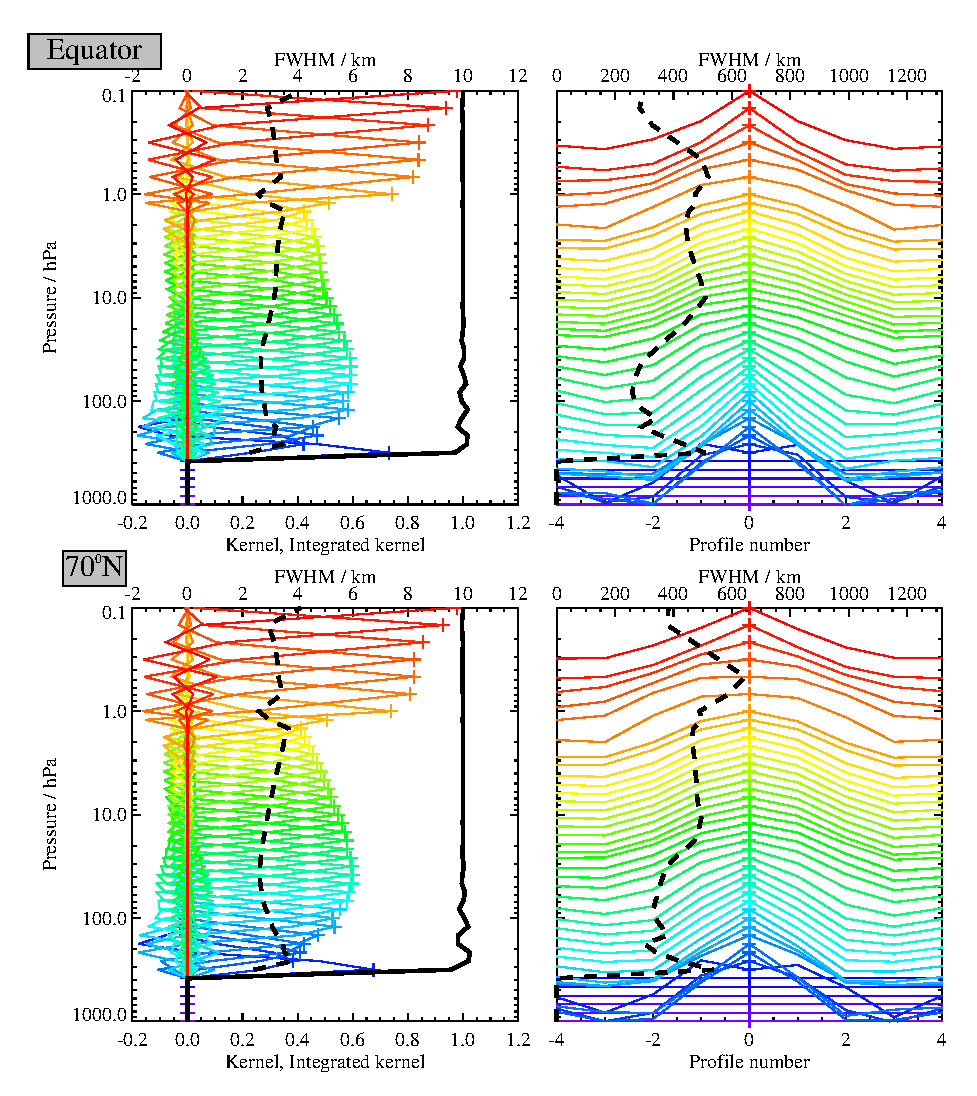
\includegraphics[width=3.5in]{figures/avk-O3_HR}\RenderNavBar}
\pagenumbering{roman}

\maketitle
%
\renewcommand{\chaptermark}[1]{%
   \markboth{\chaptername\ \thechapter.\ #1}{}}
\renewcommand{\sectionmark}[1]{%
   \markright{\thesection.\ #1}{}}
%
% --------------------------------------- Headers / footers
%
\renewcommand{\headrulewidth}{0.5pt}
\renewcommand{\footrulewidth}{0.5pt}
%
\pagestyle{fancyplain}
\renewcommand{\chaptermark}[1]{%
   \markboth{\chaptername\ \thechapter.\ #1}{}}
\renewcommand{\sectionmark}[1]{%
   \markright{\thesection.\ #1}{}}
\rhead{\large\sffamily\textcolor{HeaderFooterColor}{\nouppercase{\rightmark}}}
\lhead{}
\cfoot{%\RenderNavBar%
\sffamily\textcolor{HeaderFooterColor}{\thepage}}
\lfoot{\sffamily\textcolor{HeaderFooterColor}{Aura Microwave Limb Sounder (MLS)}}
\rfoot{\sffamily\textcolor{HeaderFooterColor}{\myshorttitle}}
%
\fancypagestyle{plain}{%
  \fancyhead{}
  \cfoot{%\RenderNavBar%
    \sffamily\textcolor{HeaderFooterColor}{\thepage}}
  \renewcommand{\headrulewidth}{0pt}
  \renewcommand{\footrulewidth}{0.5pt}
}
%
\makeatletter
\def\headrule{{\color{HeaderFooterColor}\if@fancyplain\let\headrulewidth\plainheadrulewidth\fi
   \hrule\@height\headrulewidth\@width\headwidth \vskip-\headrulewidth}}

\def\footrule{{\color{HeaderFooterColor}\if@fancyplain\let\footrulewidth\plainfootrulewidth\fi
   \vskip-\footruleskip\vskip-\footrulewidth
   \hrule\@width\headwidth\@height\footrulewidth\vskip\footruleskip}}
\makeatother
%
% --------------------------------------- Document proper
%
\clearpage
\renewcommand{\currentnav}{Help}
\RenderNavBar
\newlength{\navguidewidth}%
\setlength{\navguidewidth}{0.8\linewidth}%
\newlength{\navguidegap}%
\setlength{\navguidegap}{1.3cm}%
\thispagestyle{plain}%

\noindent\parbox{\navguidewidth}{%
\section*{Navigating this document}
\label{sec:NavGuide}

\tikzset{guidearrow/.style={ultra thick, color=DarkGreen,
    arrows=-stealth, rounded corners=3mm}}
\tikzset{hookoffset/.style={xshift=-1ex, yshift=0.5ex}}
\begin{tikzpicture}[remember picture, overlay]
  \coordinate (NBGOrigin) at
  ($ (current page.south west) + (8in, 10.7in) - (4mm, 0mm) $);
  \coordinate (HelpTarget) at ($ (NBGOrigin) - (-1.5mm, 5.5mm) $);
  \coordinate (OverviewTarget) at ($ (NBGOrigin) - (0mm, 19mm) $);
  \coordinate (MainTableTarget) at ($ (NBGOrigin) - (0mm, 33mm) $);
  \coordinate (STarget) at ($ (NBGOrigin) + (5.8mm, -11.90cm) $);
  \coordinate (TTarget) at ($ (NBGOrigin) + (5.8mm, -14.70cm) $);
\end{tikzpicture}%

Clicking on ``Help'' takes you back to this page.
\begin{tikzpicture}[remember picture, overlay]
  \node [hookoffset] (HelpHook) {};
  \draw [guidearrow] (HelpHook) -| ($ (HelpTarget-|OverviewTarget) - (3cm,0) $) -- (HelpTarget);
\end{tikzpicture}

\vspace{\navguidegap} An \hyperref[chap:Overview]{overview of the information in this
  document} is given on the next page.  You can return to it by clicking
on the ``Overview'' tab in the navigation bar.
\begin{tikzpicture}[remember picture, overlay]
  \node [hookoffset] (OverviewHook) {};
  \draw [guidearrow] (OverviewHook) -| ($ (OverviewTarget) - (2cm,0) $) -- (OverviewTarget);
\end{tikzpicture}

\vspace{\navguidegap} First time users of MLS data are advised to read
\hyperref[chap:Essential]{Chapter~\ref*{chap:Essential}} first.  The
discussion includes \hyperref[tab:ProductSummary]{a table summarizing
  key aspects of each MLS product.}  This table can be accessed from
anywhere in the document by clicking on the ``Table'' tab in the
navigation bar.
\begin{tikzpicture}[remember picture, overlay]
  \node [hookoffset] (MainTableHook) {};
  \draw [guidearrow] (MainTableHook) -| ($ (MainTableTarget) - (1cm,0) $) -- (MainTableTarget);
\end{tikzpicture}

\vspace{\navguidegap}
\hyperref[chap:Results]{Chapter~\ref*{chap:Results}} describes each of
the MLS data products individually.  You can use the navigation bar to
skip immediately to any of the product-specific sections.
\begin{tikzpicture}[remember picture, overlay]
  \node [hookoffset] (ProductHook) {};
  \draw [guidearrow] (ProductHook) -- (ProductHook-|MainTableTarget);
\end{tikzpicture}

\vspace{2ex}Each section includes
\begin{itemize}
\item A set of rules for screening out data points not recommended for
  scientific use.
\begin{tikzpicture}[remember picture, overlay]
  \node [hookoffset] (SHook) {};
  \draw [guidearrow] (SHook) -| ($ (STarget-|OverviewTarget) - (2cm,0) $) coordinate (Bend) -- (STarget);
\end{tikzpicture}
\item A table summarizing the precision, accuracy, resolution for each MLS product.
\begin{tikzpicture}[remember picture, overlay]
  \node [hookoffset] (THook) {};
  \draw [guidearrow] (THook) -- (THook-|Bend) |- (TTarget);
\end{tikzpicture}
\end{itemize}
Clicking on the product name in the navigation bar takes you to the
beginning of that section; clicking on the ``S'' and ``T'' symbols takes
you directly to the screening rules and summary table, respectively, for
that product.}

\vfill
\noindent\parbox{\navguidewidth}{%
\section*{Acknowledgment}
This research was carried out at the Jet Propulsion Laboratory,
California Institute of Technology, under a contract with the National
Aeronautics and Space Administration.}
\clearpage

%%% Local Variables: 
%%% mode: latex
%%% TeX-master: "v4-x-report"
%%% End: 
 \rhead{\large\sffamily\textcolor{HeaderFooterColor}{\nouppercase{\rightmark}}}
\lhead{}
\cfoot{\RenderNavBar%
\sffamily\textcolor{HeaderFooterColor}{\thepage}}
\lfoot{\sffamily\textcolor{HeaderFooterColor}{Aura Microwave Limb Sounder (MLS)}}
\rfoot{\sffamily\textcolor{HeaderFooterColor}{\myshorttitle}}
%
\fancypagestyle{plain}{%
  \fancyhead{}
  \cfoot{\RenderNavBar%
    \sffamily\textcolor{HeaderFooterColor}{\thepage}}
  \renewcommand{\headrulewidth}{0pt}
  \renewcommand{\footrulewidth}{0.5pt}
}
%
% Do the quick summary
%
\chapter*{Where to find answers to key questions}
\renewcommand{\currentnav}{Overview}
\setlength{\columnsep}{8mm}
\setlength{\columnseprule}{0.5pt}
\label{chap:Overview}

\begin{multicols}{2}
  
  This document serves two purposes.  Firstly, to summarize the quality
  of version~4.x Aura MLS Level~2 data.  Secondly, to convey important
  information on how to read and interpret the data to the scientific
  community.
  
  The MLS science team strongly encourages users of MLS data to
  thoroughly read this document.  Chapter~\ref{chap:Essential} describes
  essential general information for all users.
  Chapter~\ref{chap:Background} is considered background material that
  may be of interest to data users.  Chapter~\ref{chap:Results}
  discusses individual MLS data products in detail.
  
  For convenience, this page provides information on how to quickly
  ascertain answers to anticipated key questions.

  \subsection*{Where do I get \thisv MLS Level~2 data?}
  All the MLS Level~2 data described here can be obtained from the NASA
  Goddard Space Flight Center Data and Information Services Center
  (GSFC-DISC, see
  \href{http://disc.gsfc.nasa.gov/}{\texttt{http://disc.gsfc.nasa.gov/}}).

\subsection*{What format are MLS Level~2 data files in?  How do I read
  them?}

MLS Level~2 data are in HDF-EOS version~5 format.  Details are given in
section~\ref{sec:FilesAndFormats} (page~\pageref{sec:FilesAndFormats}).

\subsection*{Which MLS data points should be avoided?  How much should I trust
  the remainder?}

These issues are described in section~\ref{sec:StatusQuality} (starting
on page~\pageref{sec:StatusQuality}), and on a product by product basis
in chapter~\ref{chap:Results}.  The key rules are:
\begin{itemize}[leftmargin=2ex]
\item Only data within the appropriate pressure range (described product
  by product in chapter~\ref{chap:Results}) are to be used.
\item Always consider the precision of the data, as reported in the
  \texttt{L2gpPrecision} field.
\item Do not use any data points where the precision is zero or a
  negative number.  This indicates poor information yield from MLS.
\item Do not use data for any profile where the field \texttt{Status} is
  an odd number.
\item Data for profiles where the \texttt{Status} field is non zero
  should be approached with caution.  See
  section~\ref{sec:StatusQuality} on page~\pageref{sec:StatusQuality},
  and the product by product description in chapter~\ref{chap:Results}
  for details on how to interpret the \texttt{Status} field.
\item Do not use any data for profiles where the \texttt{Quality} field
  is \emph{smaller} than the threshold given in the section of
  chapter~\ref{chap:Results} describing your product of interest.
\item Do not use any data for profiles where the \texttt{Convergence}
  field is \emph{larger} than the threshold given in the section of
  chapter~\ref{chap:Results} describing your product of interest.
\item Some products require additional screening to remove biases or
  outliers, as described in chapter~\ref{chap:Results}.
\item Information on the accuracy of each product is given in
  Chapter~\ref{chap:Results}.  In the current (early) version of this
  document, the numbers given are for the previous v3.3 dataset.  This
  document will be updated with the specific \thisv accuracy estimates
  at a later date.
\item Data users are strongly encouraged to contact the MLS
  science team to discuss their anticipated usage of the data, and are
  always welcome to ask further data quality questions.
\end{itemize}

\subsection*{Why do some species abundances show negative values, and how do I
  interpret these?}

Some of the MLS measurements have a poor signal to noise ratio for
individual profiles.  Radiance noise can naturally lead to some negative
values for these species.  It is critical to consider such values in
scientific study.  Any analysis that involves taking some form of
average will exhibit a high bias if the points with negative mixing
ratios are ignored.

\end{multicols}


%%% Local Variables: 
%%% mode: latex
%%% TeX-master: "v4-x-report"
%%% End: 
 %
% Do the revision history
%
\chapter*{A note about revision history}
\renewcommand{\currentnav}{BLANK}

\section*{Version 4.x-0.1}
A pre-release version of the document, starting from the most recent
version 3 document.

\section*{Version 4.x-1.0}
The first publicly released version of this document.  Released when the
MLS v4.20 data set was made publicly available.

\section*{Version 4.x-2.0}
The second publicly released version of the document.  This describes
the minor changes associated with v4.22 (which fixes an issue that gave
poor temperature profiles at the end of many days).  In addition, this
version also include minor corrections and updates (notably a fix to the
averaging kernel plots which had the tropical and 70\degsym N cases
swapped).


%%% Local Variables: 
%%% mode: latex
%%% TeX-master: "v4-x-report"
%%% End: 
 %
% Now do the table of contents etc.
%
\tableofcontents
%
% ------------------------------------------------------------------------------
%
% Now call in the various chapters
%
\clearpage
%
\renewcommand{\topfraction}{0.9}
\renewcommand{\bottomfraction}{0.9}
\renewcommand{\textfraction}{0.1}
%
\pagenumbering{arabic}
\chapter{Essential reading for users of MLS version~4.x data}
\label{chap:Essential}

\section{Scope and background for this document}

This document describes the quality of the geophysical data products
produced by version~4.x of the data processing algorithms for the Earth
Observing System (EOS) Microwave Limb Sounder (MLS) instrument on the
Aura spacecraft.  The intended audience is those wishing to make use of
Aura MLS data for scientific study.  The geophysical products described
in this document are all produced by the ``Level~2'' algorithms, and
briefly summarized in Table~\ref{tab:ProductSummary}.

The \thisv MLS data are the fourth ``public release'' of MLS data, the
first being version~1.5 \citep{EOSMLSV15Quality}, the second
version~2.2, and the third versions 3.3 and 3.4.  The v2.2 data are
described in a series of validation papers published in a special issue
of the \emph{Journal of Geophysical Research} in 2007/2008.  This
document updates findings from these papers for \thisv, and gives more
general information on the use of MLS data.  As always, those wishing to
use MLS data are advised to consult the MLS science team concerning
their intended use.

%
\newenvironment{tablenotes}{%
  \begin{list}{}{%
      \renewcommand{\makelabel}[1]{##1}%
      \setlength{\itemsep}{0.5ex}%
      \setlength{\topsep}{0.5ex}%
      \setlength{\parskip}{0pt}%
      \setlength{\partopsep}{0pt}%
      \setlength{\parsep}{0pt}%
      \setlength{\itemindent}{0em}%
      \setlength{\leftmargin}{1.5em}%
      \setlength{\labelwidth}{1.5em}%
      \setlength{\labelsep}{0pt}%
    }}%
  {\end{list}}
\newcommand{\tabnudge}[1]{\smash{\raisebox{1.4ex}{#1}}}
%
\begin{table}
\renewcommand{\thefootnote}{\sffamily[\arabic{footnote}]}
\renewcommand{\arraystretch}{1.3}
%
\caption{Summary of key information for each MLS standard product.
  Essential additional information is given in each product section of
  chapter~\ref{chap:Results}.}
\label{tab:ProductSummary}
\vspace{-2mm}
%
\begin{center}
\small\sffamily
\begin{tabular}{lllllll}
\toprule
\rule[-2.5ex]{0pt}{6ex}\textbf{Product name} & 
\parbox{2.5cm}{\raggedright\bfseries Useful vertical range~/~hPa} &
\parbox{2.2cm}{\raggedright\bfseries \texttt{Quality} threshold\,\footnotemark[1]} &
\parbox{2.2cm}{\raggedright\bfseries \texttt{Convergence} threshold\,\footnotemark[2]} &
\textbf{Notes} &
\textbf{Contact name} \\
\midrule
%
\flipfloprow
\hyperref[sec:StandardBrO]{\texttt{BrO}} & 10\,--\,3.2 & 1.3 & 1.05 & A,D,N & Luis Mill\'an Valle \\
%
\flipfloprow 
\hyperref[sec:StandardCH3Cl]{\texttt{CH3Cl}} & 147\,--\,4.6 &  1.3 & 1.05 & N & Michelle Santee \\
%
\flipfloprow 
\hyperref[sec:StandardCH3CN]{\texttt{CH3CN}} & 46\,--\,1.0 &  1.4 & 1.05 & E,N & Michelle Santee \\
%
\flipfloprow 
\hyperref[sec:StandardCH3OH]{\texttt{CH3OH}} & \multicolumn{4}{c}{Not to be used pending further validation} & Michelle Santee \\
%
\flipfloprow 
\hyperref[sec:StandardClO]{\texttt{ClO}} & 147\,--\,1.0 & 1.3 & 1.05 & B & Michelle Santee \\
%
\flipfloprow 
& 100\,--\,0.0046 & & & & Hugh Pumphrey \\
\samecolorrow
\tabnudge{\hyperref[sec:StandardCO]{\texttt{CO}}}  & 215\,--\,146 & \tabnudge{1.5} & \tabnudge{1.03} & \tabnudge{C} & Michael Schwartz \\
%
\flipfloprow 
 & 83\,--\,0.001 & 0.2 & & -- &  \\
%
\samecolorrow
\tabnudge{\hyperref[sec:StandardGPH]{\texttt{GPH}}} & 261\,--\,100 & 0.9 & \tabnudge{1.03} & C,O & \tabnudge{Michael Schwartz} \\
%
\flipfloprow & 83\,--\,0.002 & & & -- & Alyn Lambert \\
\samecolorrow
\tabnudge{\hyperref[sec:StandardH2O]{\texttt{H2O}}} & 316\,--\,100 & \tabnudge{1.45} & \tabnudge{2.0} & C &
William Read \\
%
\flipfloprow 
\hyperref[sec:StandardHCl]{\texttt{HCl}} & 100\,--\,0.32 & 1.2 & 1.05 & -- & Lucien Froidevaux \\
%
\flipfloprow 
\hyperref[sec:StandardHCN]{\texttt{HCN}} & 21\,--\,0.1 & 0.2 & 2.0 & A,E,N & Hugh Pumphrey \\
%
\flipfloprow 
\hyperref[sec:StandardHNO3]{\texttt{HNO3}} & 215\,--\,1.5 & See text & See text & C,O & Gloria Manney \\
%
\flipfloprow 
\hyperref[sec:StandardHO2]{\texttt{HO2}} & 22\,--\,0.046 & N/A & 1.1 & A,D,N & Shuhui Wang \\
%
\flipfloprow 
\hyperref[sec:StandardHOCl]{\texttt{HOCl}} & 10\,--\,2.2 & 1.2 & 1.05 & N &  Lucien Froidevaux \\
%
\flipfloprow 
\hyperref[sec:StandardIWC]{\texttt{IWC}} & 215\,--\,83 & N/A & N/A & B & Alyn Lambert \\
%
\flipfloprow 
\hyperref[sec:StandardIWP]{\texttt{IWP}} & N/A & N/A & N/A & B & Alyn Lambert \\
%
\flipfloprow 
\hyperref[sec:StandardN2O]{\texttt{N2O}} & 68\,--\,0.46 & 1.3 & 2.0 & -- & Alyn Lambert \\
%
\flipfloprow 
 & 100\,--\,0.02 & & & & Lucien Froidevaux \\
%
\samecolorrow
\tabnudge{\hyperref[sec:StandardO3]{\texttt{O3}\,\footnotemark[3]}} & 
 261\,--\,121 & \tabnudge{1.0} & \tabnudge{1.03} & \tabnudge{C} &
  Michael Schwartz \\
%
\flipfloprow 
\hyperref[sec:StandardOH]{\texttt{OH}} & 32\,--\,0.0032 & N/A & 1.1 & D & Shuhui Wang \\
%
\flipfloprow 
\hyperref[sec:StandardRHI]{\texttt{RHI}\,\footnotemark[4]} & 316\,--\,0.002 & See text & See text & C,O & William Read \\
%
\flipfloprow 
\hyperref[sec:StandardSO2]{\texttt{SO2}} & 215\,--\,10 & 0.95 & 1.03 & E & William Read \\
%
\flipfloprow 
 & 83\,--\,0.001 & 0.2 & & -- &  \\
%
\samecolorrow
\tabnudge{\hyperref[sec:StandardTemperature]{\texttt{Temperature}\,\footnotemark[5]}} & 261\,--\,100 & 0.9 & \tabnudge{1.03} & C,O & \tabnudge{Michael Schwartz} \\
%
\bottomrule
\end{tabular}
\end{center}
%
\vspace{-2mm}\parbox[t]{0.5\textwidth-0.5\columnsep}{\footnotesize\sffamily
  \textbf{Notes:}\par
  \begin{tablenotes}
  \item[A] Users should consider using alternative versions of this
    product, produced using different algorithms, as described in the text.
  \item[B] This product has significant biases in certain regions
    that may need to be accounted or corrected for in scientific studies.
    See text for details.
  \item[C] Interference from clouds can affect this product at certain
    altitudes. See text for details.
  \item[D] Biases in this product can be ameliorated (in selected
    conditions) by taking day/night differences.  See text.
  \item[E] At some altitudes, this product contains biases of a magnitude
    that render the product useful only for the study of ``enhancement
    events'' (e.g., volcanic plumes, extreme fire pollution).  See text
    for details.
  \end{tablenotes}}%
\hfill\parbox[t]{0.5\textwidth-0.5\columnsep}{\footnotesize\sffamily
  \begin{tablenotes}
  \item[N] This is a ``noisy'' product requiring significant averaging
    (e.g., monthly zonal mean).  See text for details.
  \item[O] This product contains significant outliers (e.g., spikes or
    oscillations) in some regions (typically related to clouds in the
    tropical upper troposphere).  These should be screened out as detailed
    in the text.
  \end{tablenotes}
  \vspace{-1ex}\rule{\linewidth}{0.5pt}\par
  \vspace{-0.5ex}\begin{tablenotes}
  \item[\mbox{[1]}] Only use profiles with \texttt{Quality} \emph{greater}
    than this value.
  \item[\mbox{[2]}] Only use profiles with \texttt{Convergence} \emph{less} than this value.
  \item[\mbox{[3]}] File also contains a swath giving the column
    abundance above the (MLS-defined) tropopause.
  \item[\mbox{[4]}] Relative humidity with respect to ice computed from the
    MLS H\cs2O and Temperature data.
  \item[\mbox{[5]}] File also contains a swath giving tropopause
    pressure (WMO definition) inferred from MLS temperatures.
  \end{tablenotes}}

\end{table}

%%% Local Variables: 
%%% mode: latex
%%% TeX-master: "v4-x-report"
%%% End: 
 
In addition to describing the data quality, this document gives a brief
outline of the algorithms used to generate these ``Level~2'' data
(geophysical products reported along the instrument track) from the
input ``Level~1'' data (calibrated microwave radiance observations).

More information on the MLS instrument can be found in the document
\emph{An Overview of the EOS MLS Experiment} \citep{EOSMLSOverview}.  A
more general discussion of the microwave limb sounding technique and an
earlier MLS instrument is given in \citet{WatersEtal99}.  The
theoretical basis for the Level~2 software is described in
\citet{EOSMLSL2ATBD}.  A crucial component of the Level~2 algorithms is
the ``Forward Model'', which is described in detail in
\citet{EOSMLSFWMATBD} and \citet{EOSMLSPolarizedFWMATBD}.  The document
\emph{EOS MLS Retrieved Geophysical Parameter Precision Estimates}
\citep{EOSMLSPrecision} is a very useful source of information on the
expected precision of the EOS MLS data, and should be regarded as a
companion volume to this document.  The impact of clouds on MLS
measurements and the use of MLS data to infer cloud properties is
described in \cite{EOSMLSCloudATBD}.  All the above documents and papers
are available from the MLS web site (\texttt{http://mls.jpl.nasa.gov/}).

A subset of the information in these documents is also reported in the
\emph{IEEE Transactions on Geoscience and Remote Sensing}.  An overview
of MLS is given in \cite{WatersEtal06}, the algorithms that produce the
data described here are reviewed in \citet{LiveseyEtal06},
\citet{ReadEtal06}, \citet{SchwartzEtal06}, and \citet{WuEtal06}\@.
Other papers describe the calibration and performance of the various
aspects of the MLS instrument
\citep{JarnotEtal06,Pickett06,CofieldAndStek06} and the MLS ground data
system \citep{CuddyEtal06}.  The detailed validation of the MLS v2.2
dataset is described in a collection of papers in the ``Aura
Validation'' special issue of JGR-Atmospheres (papers published in 2007
and 2008).  These are cited in Chapter~\ref{chap:Results} on a
product-by-product basis.

\section{Overview of \thisv and this document}

The remainder of this chapter reviews issues that are considered
\emph{essential reading} for users of the \thisv dataset.
Chapter~\ref{chap:Background} details relevant aspects of the MLS
instrument design and operations and the theoretical basis for the \thisv
algorithms that are considered \emph{background reading}.

Chapter~\ref{chap:Results} describes the data quality for ``Standard''
products from the MLS instrument for \thisv.  These are observations of
vertical profiles of the abundance of BrO, CH\cs3Cl, CH\cs3CN, CH\cs3OH
(a new product on \thisv) ClO, CO, H\cs2O, HCl, HCN, HNO\cs3, HO\cs2,
HOCl, N\cs2O, O\cs3, and OH and SO\cs2, along with temperature,
geopotential height, relative humidity (deduced from the H\cs2O and
temperature data), cloud ice water content and cloud ice water path, all
described as functions of pressure.  In \thisv these profiles are mostly
output on a grid that has a vertical spacing of six surfaces per decade
change in pressure (\texttildelow2.5\,km), thinning out to three
surfaces per decade above 0.1\,hPa.  Exceptions to this are water vapor,
temperature, ozone and relative humidity which are on a finer 12 per
decade grid from 1000\,hPa to 1\,hPa.  Cloud ice water content is also
reported on this fine grid, though these profiles do not extend to the
stratosphere and mesosphere.  The OH product maintains a 6 per decade
grid spacing into the upper mesosphere.  Horizontally the profiles are
spaced by 1.5\degsym\ great-circle angle along the orbit, which
corresponds to about 160\,km.  The true vertical and along-track
horizontal resolution of the products is typically somewhat coarser than
the reporting grid described here.  For some of the products, the signal
to noise ratio is too low to yield scientifically useful data from a
single MLS profile observation.  In these cases, some form of averaging
(e.g.,\ weekly maps, monthly zonal means etc.) will be required to
obtain more useful results.

In addition to these standard products, the algorithms also produce data
for many ``diagnostic'' products.  The bulk of these are similar to the
standard products, in that they represent vertical profiles of retrieved
species abundances.  However, the information on these diagnostic
products has typically been obtained from a different spectral region
than that used for the standard products.  These diagnostic products are
not discussed in this document.  Further information on these is
available from the MLS science team.

At the time of writing, the current version of the data processing
software is version~4.20, producing files labeled \texttt{v04-20}.  Any
minor updates for bug fixes, or to reflect changes in input data such as
the analysis fields used as \emph{a priori} information for temperature
will be referred to as v4.21, v4.22, etc.  This version of the document
is intended to be applicable to any v4.2\emph{x} data files.  More
substantial changes at a later date (e.g., due to a change in the MLS
instrument performance) may necessitate a larger change in the data
processing software and/or its configuration.  These will be numbered
v4.3\emph{x} etc., and will be accompanied by an updated version of this
document (though not necessarily immediately, depending on the
circumstances dictating the update).

\section{MLS data validation status}

As discussed above, a complete set of MLS validation papers describe the
validation state of the earlier v2.2 data.  The majority of the v2.2 MLS
data products have, accordingly, completed ``Stage~3 Validation''
defined\footnote{See
  \href{http://science.nasa.gov/earth-science/earth-science-data/data-maturity-levels/}%
  {\texttt{http://science.nasa.gov/earth-science/earth-science-data/data-maturity-levels/}}}
as:
\begin{quote}\itshape
  Product accuracy has been assessed.  Uncertainties in the product and
  its associated structure are well quantified from comparison with
  reference in situ or other suitable reference data. Uncertainties are
  characterized in a statistically robust way over multiple locations
  and time periods representing global conditions.  Spatial and temporal
  consistency of the product and with similar products has been
  evaluated over globally representative locations and periods.  Results
  are published in the peer-reviewed literature.
\end{quote}
Work, including that described in this document, is underway to
re-validate the \thisv data, and to further establish them as ``Stage~4''
validated, defined as:
\begin{quote}\itshape
  Validation results for stage~3 are systematically updated when new
  product versions are released and as the time-series expands.
\end{quote}

\section{Differences between MLS \thisv data and earlier v3.x data}
\label{sec:V4vsV3Overview}

The MLS \thisv data processing software includes a wide range of updates
and changes, leading to differences ranging from significant to minor in
all the MLS data products.  Some of the most important are detailed
below.

\begin{description}
\item[Improved composition profiles in cloudy regions:] For the earlier
  \prevv datasets, several products (notably O\cs3, CO and HNO\cs3)
  showed poor behavior in regions of thick clouds in the upper
  troposphere (mainly in the tropics).  Complex screening approaches
  enabled users to remove many, but not all of these spurious profiles
  from consideration.  Improved performance in this regard was a key
  goal for \thisv, and the manner in which contamination from cloud
  signals is handled in the MLS gas-phase retrievals was substantially
  modified.  This has resulted not only in a significant reduction in
  the number of spurious MLS profiles reported in cloudy regions, but
  also in an appreciable simplification of the steps users need to take
  to screen out the most cloud-contaminated measurements, and a more
  effective screening.

\item[Improvements to O\cs3 and HCN:] The MLS O\cs3 and HCN products
  have been improved in \thisv through addition of specific retrieval
  ``phases'' dedicated to obtaining more accurate estimates for these
  products, and reducing the impact of contaminating signals from other
  species.

\item[Improvements to H\cs2O:] The MLS H\cs2O product is retrieved in
  two ``phases'' with a preliminary phase obtaining a
  coarse-vertical-resolution initial guess and informing the choice of
  smoothing constraint for a subsequent more detailed high-resolution
  retrieval.  The use of more channels and more accurate forward model
  calculations in this initial retrieval have led to improvements in the
  convergence etc. of the second phase, and thus to improvements in the
  H\cs2O product.

\item[New CH\cs3OH product:] This product, obtained from measurements in
  the 190- and 640-GHz spectral regions (also from a dedicated retrieval
  ``phase''), has been introduced in \thisv.  This product is
  scientifically useful in the tropical upper troposphere (see
  section~\ref{sec:StandardCH3OH}).

\item[More suitable reference surface for geopotential height:] As of
  \thisv, the MLS geopotential height (GPH) product has been redefined
  to be GPH from a reference geoid (a surface of constant geopotential)
  rather than from an ellipsoid, as was used in previous versions.

\item[More useful OH retrievals for recent years:] As discussed in
  section~\ref{sec:OHNote}, MLS observations of OH have been made only
  sparingly in recent years in light of increased aging in the MLS
  ``THz'' subsystem making that measurement.  Updates in the \thisv
  algorithms have enabled a greater yield of useful OH profiles in the
  more recent years of observations affected by this aging than was the
  case in \prevv.
\end{description}

In addition to these specific changes, changes in all products,
including those not listed above, have resulted from updates to
spectroscopy and instrument calibration knowledge, and in indirect
response to the larger changes detailed above.  Note that the threshold
values of ``\texttt{Quality}'' and ``\texttt{Convergence}'' (see below)
to be used in data screening have been updated for all products.  All
the standard product files (apart from IWC, see below) now also include
the \emph{a priori} information used in the retrieval (as an additional
``swath'', see below).

\section{Aura MLS file formats, contents, and first order
  quality information}
\label{sec:FilesAndFormats}
\label{sec:NegativePrecision}

All the MLS Level~2 data files described here are available from the
NASA Goddard Space Flight Center Data and Information Services Center
(GSFC-DISC, see
\href{http://disc.gsfc.nasa.gov/}{\texttt{http://disc.gsfc.nasa.gov/}}).
The standard and diagnostic products are stored in the EOS MLS
\emph{Level 2 Geophysical Product} (L2GP) files.  These are standard
HDF-EOS (version~5) files containing swaths in the Aura-wide standard
format.  For more information on this format see
\citet{AuraFileConventions}.  A sample reading function for the
Interactive Data Language (IDL, version 6.1 or later required), known as
\texttt{readl2gp.pro} may have been supplied with the data and is
available from the \emph{Open Channel Software Foundation}
\href{http://www.openchannelsoftware.org/}{\texttt{http://www.openchannelsoftware.org/}}.
A reader for MATLAB (\texttt{readL2GP.m}) is also available at the same
site, and one for python is planned to be added shortly.

The standard products are stored in files named according to the convention
\begin{quote}
\verb+MLS-Aura_L2GP-<product>_v04-20-c01_<yyyy>d<ddd>.he5+
\end{quote}
where \verb+<product>+ is \texttt{BrO}, \texttt{O3},
\texttt{Temperature}, etc.  The files are produced on a one-day
granularity (midnight to midnight, universal time), and named according
to the observation date where \verb+<yyyy>+ is the four digit calendar
year and \verb+<ddd>+ is the day number in that year (\texttt{001} = 1
January).

These files contain the corresponding standard product in an HDF-EOS
swath given the same name as the product, e.g., ``\texttt{H2O}''.  With the
exception of IWC, each file also contains the \emph{a priori} values for that
product inside a second swath whose name ends with the substring
``\texttt{-APriori}''. HNO\cs3, IWC, O3, RHI, and Temperature files are special in
that they carry extra standard or non-standard products, as detailed in
Table~\ref{tab:SwathExtras}.

\begin{table}
  \caption{Additional swaths in specific standard product
    files.\label{tab:SwathExtras}}\small
\begin{center}
\begin{tabular}{>{\ttfamily}l>{\ttfamily}ll}
  \toprule
  \textbf{\rmfamily Product} & \textbf{\rmfamily Additional swaths} &
  \textbf{\rmfamily Notes} \\
  \midrule
  HNO3 & HNO3-190, HNO3-240 & Nitric acid from the 190 and
  240\,GHz radiometers\\
  IWC & IWP & partial Ice Water Path.  (This file has no \emph{a priori} swath) \\
  O3 & O3 column & Ozone column above the tropopause (see below) \\
  RHI & UTRHI, UTRHI-APriori & ``Single layer'' relative humidity (see Section~\ref{sec:StandardRHI})\\
  Temperature & WMOTPPressure & Tropopause (WMO definition, based MLS
  temperature) \\
  \bottomrule
\end{tabular}
\end{center}
\end{table}

The files contain an HDF-EOS swath given the same name as the product.
In addition, the standard O\cs3 product files also contain swaths
describing column abundances, and the standard Temperature file contains
additional swaths describing tropopause pressure.  As some L2GP files
contain multiple swaths, it is important to ensure that the correct
swath in the \texttt{L2GP} files is requested from the file.  In the
case where the ``default'' swath is requested (i.e., no swath name is
supplied) most HDF software will access the one whose name falls
earliest in ASCII order.  This generally results in the desired result
for all products.  For example, for temperature, the standard
``\texttt{Temperature}'' product will be read in preference to the
``\texttt{WMOTPPressure}'' swath that gives tropopause pressures.

Each swath contains data fields \texttt{L2gpValue} and
\texttt{L2gpPrecision}, which describe the value and precision of the
data, respectively.  Data points for which \texttt{L2gpPrecision} is set
negative or zero \emph{should not be used}, as this flags that the
resulting precision is worse than 50\% of the \emph{a priori} precision,
indicating that instrument and/or the algorithms have failed to provide
enough useful information for that point.  In addition to these fields,
fields such as \texttt{latitude} etc.\ describe geolocation information.
The field \texttt{time} describes time, in the EOS standard manner, as
the number of seconds elapsed (including from five to nine subsequent
leap seconds to date) since midnight universal time on 1~January 1993.

The \texttt{L2GP-DGG} (``Diagnostic products on a Geophysical Grid'')
file contains a large number of additional swath quantities.  The vast
majority of these are MLS diagnostic products that will be of little
interest to most data users.  A few which may be of interest to some
users are detailed below.

\section{Additional information given in the \texttt{Quality},
  \texttt{Convergence} and \texttt{Status} fields}
\label{sec:StatusQuality}

\usetikzlibrary{calc}
\begin{figure}[tb]
\definecolor{bitcolor}{gray}{0.80}
\newlength{\bitsize}
\setlength{\bitsize}{1.0cm}
\newlength{\meaningheight}
\setlength{\meaningheight}{-1.5cm}
\newlength{\xpos}
\setlength{\xpos}{10.6cm}
\newlength{\ypos}
\setlength{\ypos}{-1.5cm}
\begin{tikzpicture}
\small\sffamily
%
% First the bits
\begin{scope}[minimum size=\bitsize,very thick]
\node (b11) at (0\bitsize,0pt) [rectangle, draw, fill=bitcolor, label=above:10] {\small\ttfamily 1024};
\node (b9) at (1\bitsize,0pt) [rectangle, draw, fill=bitcolor, label=above:9] {\small\ttfamily 512};
\node (b8) at (2\bitsize,0pt) [rectangle, draw, fill=bitcolor, label=above:8] {\small\ttfamily 256};
\node (b7) at (3\bitsize,0pt) [rectangle, draw, fill=bitcolor, label=above:7] {\small\ttfamily 128};
\node (b6) at (4\bitsize,0pt) [rectangle, draw, fill=bitcolor, label=above:6] {\small\ttfamily 64};
\node (b5) at (5\bitsize,0pt) [rectangle, draw, fill=bitcolor, label=above:5] {\small\ttfamily 32};
\node (b4) at (6\bitsize,0pt) [rectangle, draw, fill=bitcolor, label=above:4] {\small\ttfamily 16};
\node (b3) at (7\bitsize,0pt) [rectangle, draw, fill=bitcolor, label=above:3] {\small\ttfamily 8};
\node (b2) at (8\bitsize,0pt) [rectangle, draw, fill=bitcolor, label=above:2] {\small\ttfamily 4};
\node (b1) at (9\bitsize,0pt) [rectangle, draw, fill=bitcolor, label=above:1] {\small\ttfamily 2};
\node (b0) at (10\bitsize,0pt) [rectangle, draw, fill=bitcolor, label=above:0] {\small\ttfamily 1};
% A key
\node at (11\bitsize,0pt) [rectangle, minimum size=\bitsize, label=above:Bit, align=left] {\small\ttfamily\null\hspace{1em} Value};
\end{scope}
%
% Now the meanings
\newcommand{\meaningbox}[2]{\parbox{5cm}{\raggedright\textbf{#1} #2}}
\begin{scope}[inner sep=0pt, outer sep=4pt, anchor=west]
\node (m0) at (\xpos,\ypos+0\meaningheight) {\meaningbox{Flag -- Bad Profile:}%
  {Do not use this profile (see ``information'' bits for an explanation).}};
\node (m1) at (\xpos,\ypos+1\meaningheight) {\meaningbox{Flag -- Warning:}%
  {This profile is questionable (see ``information'' bits for an explanation).}};
\node (m2) at (\xpos,\ypos+2\meaningheight) {\meaningbox{Flag -- Comment}%
  {See ``information'' bits for additional comments concerning this profile.}};
%
% Nudge a bit
%
\addtolength{\ypos}{-2mm}
\node (m4) at (\xpos,\ypos+3\meaningheight) {\meaningbox{Information:}%
  {(Warning) This profile may have been affected by high altitude clouds.}};
\node (m5) at (\xpos,\ypos+4\meaningheight) {\meaningbox{Information:}%
  {(Warning) This profile may have been affected by low altitude clouds.}};
\node (m6) at (\xpos,\ypos+5\meaningheight) {\meaningbox{Information:}%
  {(Comment) GEOS-5 \emph{a priori} temperature data were unavailable for this profile.}};
\node (m7) at (\xpos,\ypos+6\meaningheight) {\meaningbox{Information:}%
  {(Bad profile) The retrieval for this phase encountered a numerical error.}};
\node (m8) at (\xpos,\ypos+7\meaningheight) {\meaningbox{Information:}%
  {(Bad profile) Too few radiances were available for good retrieval of this profile.}};
\node (m9) at (\xpos,\ypos+8\meaningheight) {\meaningbox{Information:}%
  {(Bad profile) The task retrieving this profile crashed (typically a computer failure).}};
\end{scope}
%
% Now a separator
\draw[ultra thick] ($ (m2.west)!0.5!(m4.west) $) -- ($ (m2.east)!0.5!(m4.east) $);
% \draw[ultra thick] (0,0) -- (10,0);
%
% Now the connections
\begin{scope}[>=stealth,thick]
\draw[->] (b0) |- (m0);
\draw[->,dashed] (b1) |- (m1);
\draw[->] (b2) |- (m2);
\draw[->,dashed] (b4) |- (m4);
\draw[->] (b5) |- (m5);
\draw[->,dashed] (b6) |- (m6);
\draw[->] (b7) |- (m7);
\draw[->,dashed] (b8) |- (m8);
\draw[->] (b9) |- (m9);
\end{scope}
\end{tikzpicture}
\caption{The meaning of the various bits in the \texttt{Status} field.
  The bits not labeled are not used in \thisv.  Later versions may
  implement specific meanings for these bits.  Note that bit 6 (GEOS-5
  data) was not used in v1.5, and that the information in bits 7 and 8
  were combined into bit 8 in versions~1.5 and~2.2.}
\label{fig:StatusBits}
\end{figure}


%%% Local Variables: 
%%% mode: latex
%%% TeX-master: "v4-x-report"
%%% End: 
 
In addition to the data and their estimated precisions, three quality
metrics are output for every profile of each product.  The first, called
\texttt{Quality}, gives a measure of the quality of the product based on
the fit achieved by the Level~2 algorithms to the relevant radiances.
Larger values of \texttt{Quality} generally indicate better radiance
fits and therefore more trustworthy data. Values of \texttt{Quality}
closer to zero indicate poorer radiance fits and therefore less
trustworthy data.  The value of \texttt{Quality} to be used as a
``threshold'' for rejecting data in scientific studies varies from
product to product, and is given later in this document.

The second quality metric is called \texttt{Status}.  This is a 32 bit
integer that acts as a bit field containing several ``flags''.
Figure~\ref{fig:StatusBits} describes the interpretation of these flags
in more detail.  The first two bits (bits 0 and 1) are ``flagging''
bits.  If the first bit is set it indicates that the profile
\emph{should not be used in any scientific study}.  Accordingly, any
profile for which \texttt{Status} is an odd number should not be used.
The second bit indicates that data are considered questionable for some
reason.  Higher bits give more information on the reasons behind the
setting of the first two bits.  So, for example, a value of
\texttt{Status} of \texttt{18} (2+16) indicates that the data are
questionable (\texttt{2}\,$\equiv$\,bit 2) because of the possible
presence of high altitude clouds (\texttt{16}\,$\equiv$\,bit 4).

The most commonly set information bits are the ``high altitude cloud''
and ``low altitude cloud'' bits.  These indicate that the data have been
marked as questionable because the Level~2 software believed that the
measurements may have been affected by the presence of clouds (clouds
alone will never cause a profile to be marked as not to be used, i.e.,
with odd \texttt{Status}).  The implications of this vary from product
to product and, more importantly, height to height.  For example,
situations of either ``low cloud'' or ``high cloud'' typically have very
little impact on the quality of stratospheric data.  Further details of
the implications of these flags are given later in this document on a
product by product basis.

The third diagnostic field \texttt{Convergence} describes how the fit to
the radiances achieved by the retrieval algorithms compared to the
degree of fit to be expected.  This is quantified as a ratio of an
aggregate $\chi^2$ value to that predicted based on the assumption of a
linear system \citep{LiveseyEtal06}.  Values around unity indicate good
convergence, the threshold values above which profiles should not be used
are given on a product by product basis later in this document.

\section{An important note on negative values}
\label{sec:NegativeValuesOK}

Some of the MLS observations are ``noisy'' in nature.  A consequence of
this is that negative values may often be reported for species mixing
ratios.  It is important that such values \emph{not be ignored or
  masked}.  Ignoring such values will automatically introduce a positive
bias into any averages made of the data as part of scientific analysis.
Water vapor is retrieved using a logarithmic basis (both vertically and
horizontally, as discussed in section~\ref{sec:BasisIssues}).
Accordingly, no negative water vapor abundances are produced by \thisv.

\section{Averaging kernels for MLS \thisv profiles}
\label{sec:AveragingKernels}
As is common for remote sounding instruments, consideration of the
``Averaging Kernel'' \citep[e.g.,][]{Rodgers00} can be important in some
scientific studies.  However, the relatively high vertical resolution of
the MLS observations (compared, for example, to nadir sounding
composition instruments) allows for many scientifically useful studies
to be undertaken without reference to the averaging kernels.  This
section reviews the role averaging kernels play in comparing MLS
profiles to other observations and/or model profiles and describes how
to obtain representative kernels for the \thisv data.

The averaging kernel matrix $\b{A}$ relates the retrieved MLS profiles
(given by the vector $\hat{\b{x}}$) to the ``true'' atmospheric state (the
vector $\b{x}$) according to
\begin{equation}
  \b{A} = \frac{\partial\hat{\b{x}}}{\partial\b{x}}.
\end{equation}
Rows of the $\b{A}$ matrix accordingly describe the contributions of the
true atmospheric profile to the given level in the retrieved profile.
The figures later in this document show these rows as individual colored
lines.

Given an independent observation or model estimate of an atmospheric
profile $\b{x}$, the averaging kernels, in combination with the MLS
\emph{a priori} profile $\b{x}_a$, can be used to compute the profiles
that MLS would observe, were the true profile to be in the state given
by $\b{x}$, according to
\begin{equation}
  \hat{\b{x}} = \b{x}_a + \b{A}\left[\b{x}-\b{x}_a\right]
\label{eqn:AVKApplication}
\end{equation}
As of MLS version \thisv, the the \emph{a priori} profile for each MLS
observation is available within each of the standard product files, in
swaths named according to the product, with the suffix
``\texttt{-APriori}'' (note the hyphen).  Examples are
``\texttt{Temperature-APriori}'' and ``\texttt{O3-APriori}''.  This
information can also be obtained from the MLS \texttt{L2GP-DGG} files
(the only source for this information in \prevv and earlier versions).

Note that in the case of water vapor where (as described below) a
logarithmic interpolation is used for the profile, the calculations in
equation~\ref{eqn:AVKApplication} should be performed in log space,
i.e., with $\b{x}$ and $\b{x}_a$ containing logarithm of the given
H\cs2O mixing ratio (leaving the $\b{A}$ matrix as supplied).

The full MLS averaging kernels are complicated entities, reflecting the
two dimensional ``tomographic'' nature of the MLS retrievals (see
section~\ref{sec:TheoreticalBasis}).  We anticipate that few, if any,
users will need to apply these full two dimensional kernels, whose
interpretation is complex (please contact the MLS team for further
information on these).  The full kernels can be ``collapsed'' in the
horizontal, to provide a single vertical averaging kernel for each
product (as is done for many nadir sounding instruments).  Such kernels
are shown for each product (along with ``horizontal'' averaging kernels)
in chapter~\ref{chap:Results}.  The MLS averaging kernels typically
change little with latitude / season / atmospheric state.  Accordingly,
two representative kernels are shown for each product, one for the
tropics and one for polar winter conditions.  These representative
kernels are available to users as described below.  If variability in
the averaging kernels is a concern, comparison of $\hat{\b{x}}$ profiles
obtained using the two kernels (likely to represent two extreme cases)
can provide a quantitative estimate of the magnitude of differences
introduced by kernel variations.

The two averaging kernels for each product are distributed as text
files, named according to
\begin{quote}
\verb+MLS-Aura_L2AK-<product>-<case>_v04-2x_0000d000.txt+
\end{quote}
where \verb+<case>+ is \verb+Eq+ or \verb+70N+ for the equator and
70\degsym N, respectively (or \verb+Day+ and \verb+Night+ for OH, see
section~\ref{sec:StandardOH}).  These files are available from the MLS
web site at
\href{http://mls.jpl.nasa.gov/data/ak/}{\texttt{http://mls.jpl.nasa.gov/data/ak/}}.

These files contain comment lines (prefixed with a semicolon) describing
their format.  The first non-comment line gives the name of the product
and the number of levels in the vertical profile.  A list of the
pressure levels in the profile (matching those in the L2GP files) is
then given, followed by all the values of the averaging kernel matrix,
with the row index (the level in the retrieved profile) varying most
rapidly.

Typically, of course, the MLS profile pressures are not those of the
observation or model dataset to which the comparison is being made.  In
many cases, particularly where the resolution of the other dataset is
comparable to that of the MLS profiles, a simple linear interpolation is
the most practical manner in which to transform the other dataset into
the $\b{x}$ profile space.  However, we note that more formal approaches
have been described \citep{RodgersAndConnor03} for the case where the
comparison dataset is also remotely sounded and has an averaging kernel.
In cases where the comparison dataset has high vertical resolution
(e.g., sonde or Lidar observations), an additional consideration is
described in the following section.

\section{Considerations for comparisons with high vertical resolution
  datasets}
\label{sec:BasisIssues}

The MLS Level~2 data describe a piecewise linear representation of
vertical profiles of mixing ratio (or temperature, GPH, etc.) as a function of
pressure, with the tie points given in the \texttt{L2GP} files (in the
case of water vapor, the representation is piecewise linear in log
mixing ratio).  This contrasts with some other instruments, which report
profiles in the form of discrete layer means.  This interpretation has
important implications that may need to be considered when comparing
profiles from MLS to those from other instruments or models,
particularly those with higher vertical resolution.

It is clearly not ideal to compare MLS retrieved profiles with finer
resolution data by simply ``sampling'' the finer profile at the MLS
retrieval surfaces.  One might expect that instead one should do some
linear interpolation or layer averaging to convert the other dataset to
the MLS grid.  However, in the MLS case where the state vector describes
a profile at infinite resolution obtained by linearly interpolating from
the fixed surfaces, it can be shown that the appropriate thing to do is
to compare to a least squares fit of the non-MLS profile to the lower
resolution MLS retrieval grid.

Consider a high resolution profile described by the vector $\b{z}_h$,
and a lower resolution MLS retrieved profile described by the vector
$\b{x}_l$.  We can construct a linear interpolation in log pressure that
interpolates the low resolution information in $\b{x}_l$ to the high
resolution grid of $\b{z}_h$.  We describe that operation by the
(typically highly sparse) $n_h \times n_l$ matrix $\b{H}$ such that
\begin{equation}
\b{x}_h = \b{H}\b{x}_l
\label{eqn:EtaForward}
\end{equation}
where $\b{x}_h$ is the high resolution interpolation of the low
resolution $\b{x}_l$.  It can be shown that the best estimate profile
that an idealized MLS instrument could obtain, were the true atmosphere
in the state described by $\b{z}_h$, is given by
\begin{equation}
\b{z}_l = \b{W}\b{z}_h
\label{eqn:EtaBackward}
\end{equation}
where
\begin{equation}
\b{W} = \left[ \b{H}\T \b{H} \right]\inv \b{H}\T
\end{equation}
In other words, $\b{z}_l$ represents a least squares linear fit to
$\b{z}_h$. This operation is illustrated by an example in
Figure~\ref{fig:BasisExample}.  Precision uncertainty on high resolution
measurements may be similarly converted to the MLS grid by applying
\begin{equation}
\b{S}_l = \b{W} \b{S}_h \b{W}\T
\end{equation}
where $\b{S}_h$ is the covariance of the original high resolution data
(typically diagonal) and $\b{S}_l$ is its low resolution representation
on the MLS pressure grid.  Following this transfer of the
high-resolution profile onto the state vector vertical grid, the profile
can be multiplied by the averaging kernels, as described above,
according to equation~\ref{eqn:AVKApplication}.

In some cases, the application of this least-squares ``smoothing'' is as
important, if not more important, than the application of the averaging
kernels described above.  This is particularly true when the averaging
kernels are close to delta functions, indicating that the vertical
resolution is comparable to the retrieved profile level spacing.

In the case of water vapor, where a logarithmic vertical basis is used,
the $\b{x}$ and $\b{z}$ vectors should describe the logarithm of the
mixing ratio.

\begin{figure}[tb]
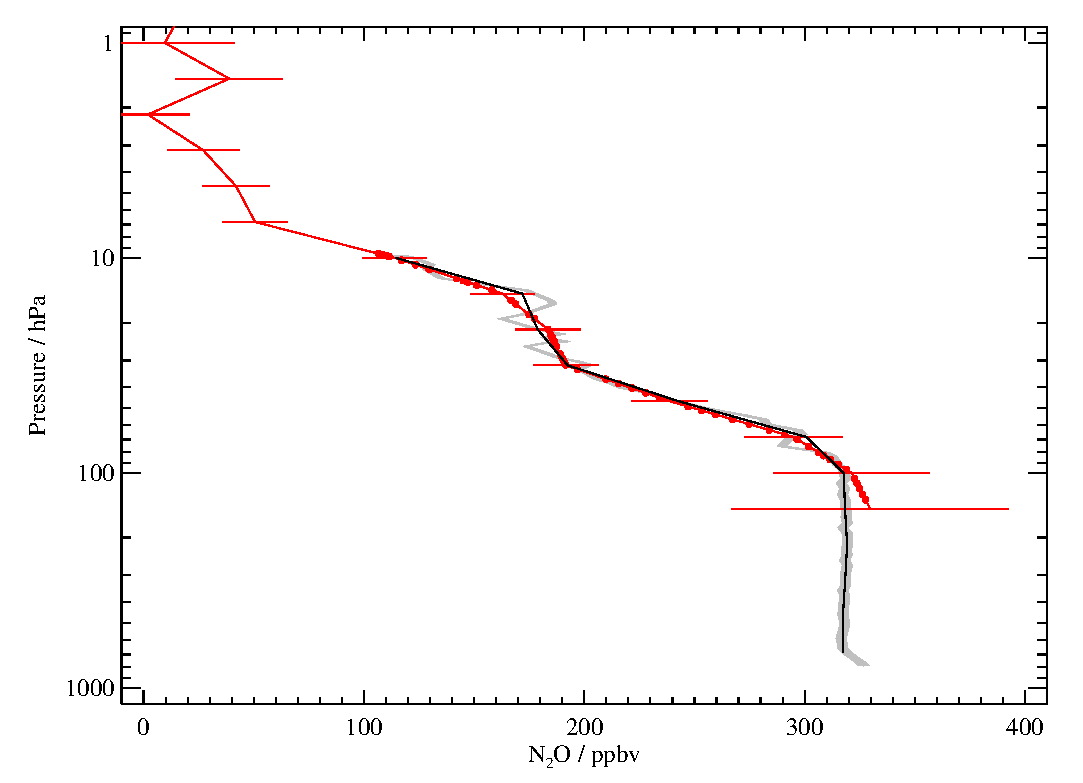
\includegraphics[width=\textwidth]{figures/basisexample}
\caption{Comparisons of MLS (v1.5) N\cs2O observations with in-situ
  balloon data (courtesy of J.~Elkins).  The raw balloon data
  ($\b{z}_h$) are shown as the grey shaded region (shading indicates
  precision).  A coincident MLS profile ($\b{x}_l$) is shown in red with
  the red error bars indicating precision.  The red dots show the MLS
  data linearly interpolated to the balloon pressures using the $\b{H}$
  matrix (i.e., $\b{x}_h$ from equation~\ref{eqn:EtaForward}).  The
  black line shows the ``least squares'' interpolation of the balloon data
  onto the MLS grid using the $\b{W}$ matrix as described in the text
  (i.e., $\b{z}_l$ from equation~\ref{eqn:EtaBackward}).  The black line
  therefore represents the closest possible match at this resolution to
  the original grey line, and is the appropriate quantity to compare to
  the red MLS profile, and to be multiplied by the averaging kernels for
  formal comparison.}
\label{fig:BasisExample}
\end{figure}

\section{A note on the HCl measurements in \thisv}

Starting in February~2006, the primary MLS band for measuring HCl
(specifically the HCl\cp{35} isotopologue) (\texttt{R4:640.B13F:HCl} or
``band~13'') began to exhibit symptoms of aging and was deactivated to
conserve life.  This is likely to be due to a radiation susceptibility
issue for a batch of transistors identified shortly before launch.
Useful observations of HCl are still made with the adjacent band
(\texttt{R4:640.B14F:O3} or ``band~14'') which, as can be seen from
Figures~\ref{fig:UnfoldedSpectra} and~\ref{fig:FoldedSpectra} also
observe the HCl\cp{35} line (and a smaller line for the HCl\cp{37}
isotopologue).

In order to avoid undesirable discontinuities in the \thisv HCl dataset,
the band~13 radiances are not considered in the retrieval of the
standard HCl product, even on days for which it was active.  For days
prior to the 16~February 2006 deactivation of band~13, and the few
subsequent days when band~13 has been (or may be) reactivated, the
\thisv algorithms also produce a second HCl product (in the
\texttt{HCl-640-B13} swath in the \texttt{L2GP-DGG}) file which includes
the band~13 radiances, giving a product with improved precision and
resolution in the upper stratosphere and mesosphere.  See
section~\ref{sec:StandardHCl} for more information.

As discussed in section~\ref{sec:StandardHCl}, while the band~14 and
band~13 data show very good agreement in the lower stratosphere, they
disagree on the magnitude of the declining trend in upper stratospheric
HCl (reflecting cuts in emissions of ozone depleting substances).  At
these high altitudes the HCl line is significantly narrower than the
single channel in band~14 in which it resides, whereas the band~13
channels (by design, as this band was targeted to HCl) resolve the line
shape.  Accordingly, the band~13 trend is judged to be the more accurate
one.

\section{A note on N\cs2O measurements in \thisv}

The preferred MLS band for measuring N\cs2O (band 12 in the 640\,GHz
region, \texttt{N2O-640}) began to show signs of aging in June 2013
(although more slowly than the rapid decline observed in the HCl band~13
in 2006). Band~12 was subsequently turned off on August 6,
2013. However, the level-2 processing stream for the N\cs2O standard
product in v3.x was switched to output the band 3 (190\,GHz,
\texttt{N2O-190}) retrieval on 7~June~2013 and later data for
\texttt{N2O-640} are not recommended for scientific use.

For v4.x the decision was taken to assign the band 3 (190\,GHz,
\texttt{N2O-190}) retrieval as the standard product from launch,
wherease the band 12 (640\,GHz, \texttt{N2O-640}) retrieval is now only
available in the \texttt{N2O-640} swath in the \texttt{L2GP-DGG} file.

As discussed in section~\ref{sec:StandardN2O}, the band~3 and band~12
data show good agreement except at 100 hPa where there is a $>$30\% high
bias in the N\cs2O values from band~3.

\section{A note on OH measurements in \thisv}
\label{sec:OHNote}

The MLS OH measurements derive from observations in the 2.5-THz region
of the spectrum. The local oscillator signal driving the MLS 2.5-THz
radiometers is provided by a methanol laser (pumped by a CO\cs2
laser). In December 2009, following more than five years of operation,
this laser began to show signs of aging and was temporarily deactivated
(prior to the 2004 Aura launch, the expected lifetime of this laser was
only eighteen months).

Upper stratospheric and mesospheric OH is strongly affected by solar
activity \citep{WangEtal13}, which was low during the solar 11-year
minimum in 2009. In order to conserve the remaining lifetime of the THz
instrument for valuable measurements when the Sun becomes more active,
we suspended OH measurements from December 2009 to August 2011.  As the
Solar Cycle 24 rises with increasing solar activity, we reactivate THz
instrument for a 30-day continuous measurement during August --
September in each year. The reasons of having this measurement at this
time of year are:
\begin{enumerate}
\item Since MLS OH measurements started in early August in 2004, in
  order to achieve the longest possible annual OH data record for trend
  studies, we have to choose a time no earlier than August.
\item The ground-based instrument used for MLS OH validation
  \citep{WangEtal08}, located at 34.4\degsym N, has the best OH
  measurement signal in summer (June -- August) and the lowest signal in
  winter. Having the annual MLS OH measurement starting in August allows
  for continuing validation with the best possible collocated
  ground-based data.
\end{enumerate}
We have performed the 30-day OH measurement in each August -- September
during 2011\,--\,2014 and plan to continue it during the declining phase
of Solar Cycle 24. However, due to the aging of the instrument, OH data
acquired since 2014 are significantly noisier than the previous years
and have poor spatial coverage at mid-low latitudes.


%%% Local Variables: 
%%% mode: latex
%%% TeX-master: "v4-x-report"
%%% End: 
 \chapter{Background reading for users of MLS version~4.x data}
\label{chap:Background}

\section{Aura MLS radiance observations}

\begin{sidewaysfigure}
  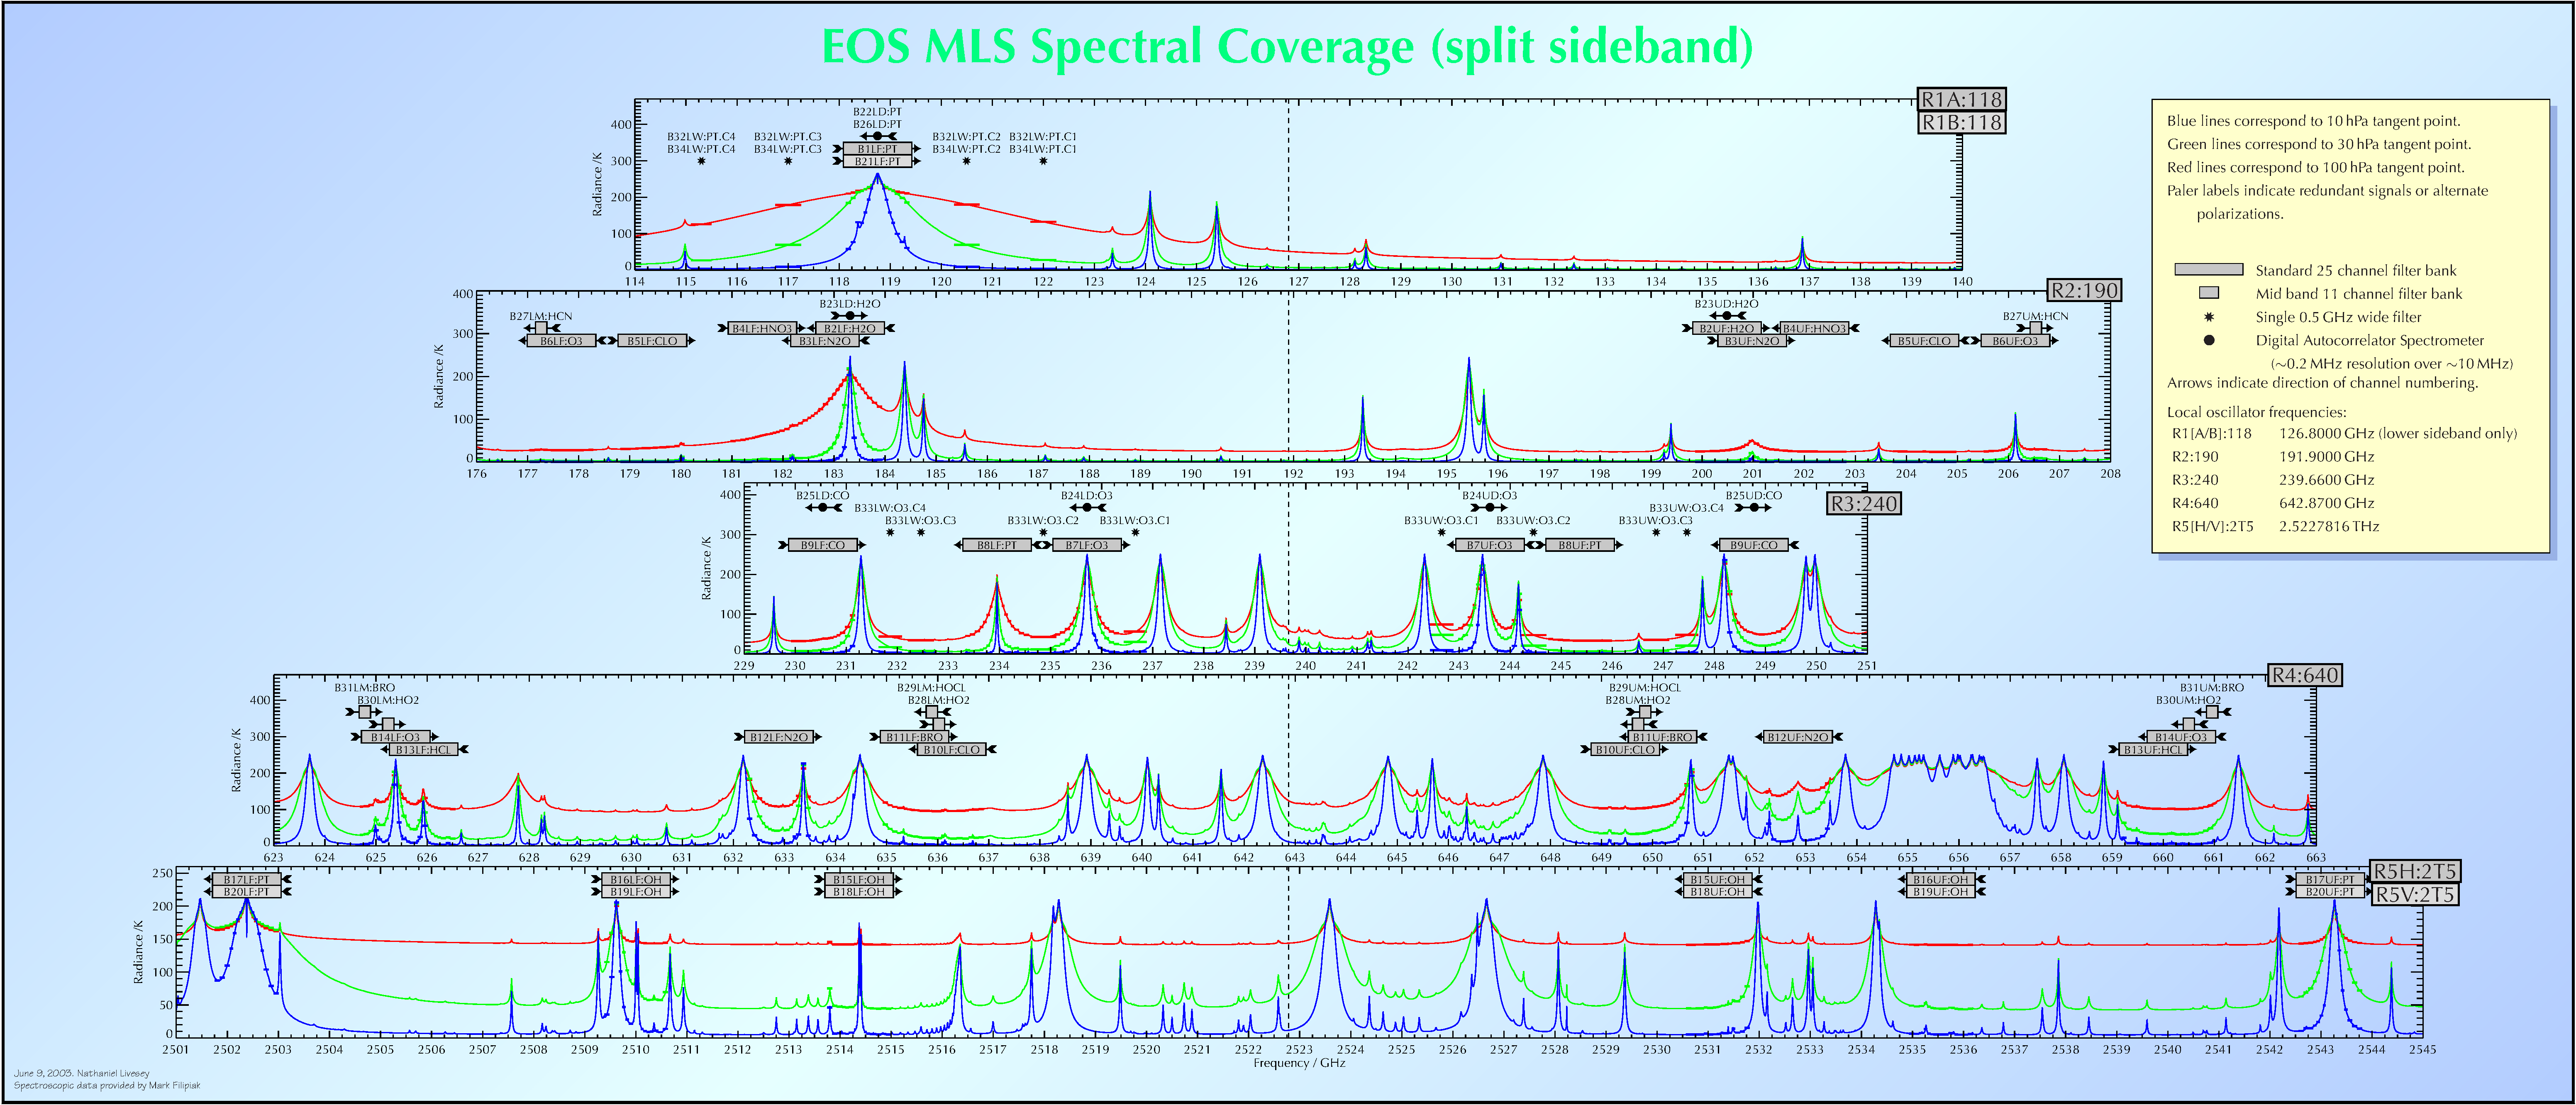
\includegraphics[width=\linewidth]{figures/unfolded-complete}
\caption{The five panels show the spectral regions covered by the MLS
  radiometers.  The grey boxes and other symbols denote the position of
  the various ``bands'' observed within the spectral regions covered by
  each radiometer.}
\label{fig:UnfoldedSpectra}
\end{sidewaysfigure}

\begin{figure}[htb]
\includegraphics[width=\linewidth]{figures/folded-complete}
\caption{This is similar to figure~\protect{\ref{fig:UnfoldedSpectra}},
  except that x-axes represent ``intermediate frequency''.  The signal at
  each intermediate frequency represents a sum of the signals observed
  at that frequency both above and below the local oscillator (below
  only in the case of the 118\,GHz receivers.)}
\label{fig:FoldedSpectra}
\end{figure}

Figures~\ref{fig:UnfoldedSpectra} and~\ref{fig:FoldedSpectra} show the
spectral coverage of the MLS instrument.  The instrument consists of
seven radiometers observing emission in the 118\,GHz (R1A and R1B),
190\,GHz (R2), 240\,GHz (R3), 640\,GHz (R4) and 2.5\,THz (R5H and
R5V) regions.  With the exception of the two 118\,GHz devices, these are
``double sideband'' radiometers.  This means that the observations from
both above and below the local oscillator frequencies are combined to
form an ``intermediate frequency'' signal.  In the case of the 118-GHz
radiometers, the signals from the upper sideband (those frequencies
above the \texttildelow126\,GHz local oscillator) are suppressed.  These
intermediate frequency signals are then split into separate ``bands''.
The radiance levels within these bands are quantified by various
spectrometers.

In operation, the instrument performs a continuous vertical scan of both
the GHz (for R1A--R4) and THz (R5H, R5V) antenn\ae\ from the surface to
about 90\,km in a period of about 20\,s.  This is followed by about 5\,s
of antenna retrace and calibration activity.  This \texttildelow25\,s cycle is
known as a \emph{Major Frame} (MAF).  During the \texttildelow20\,s continuous
scan, radiances are reported at 1/6\,s intervals known as \emph{Minor
  Frames} (MIFs).

\section{Brief review of theoretical basis}
\label{sec:TheoreticalBasis}

\begin{figure}[htb]
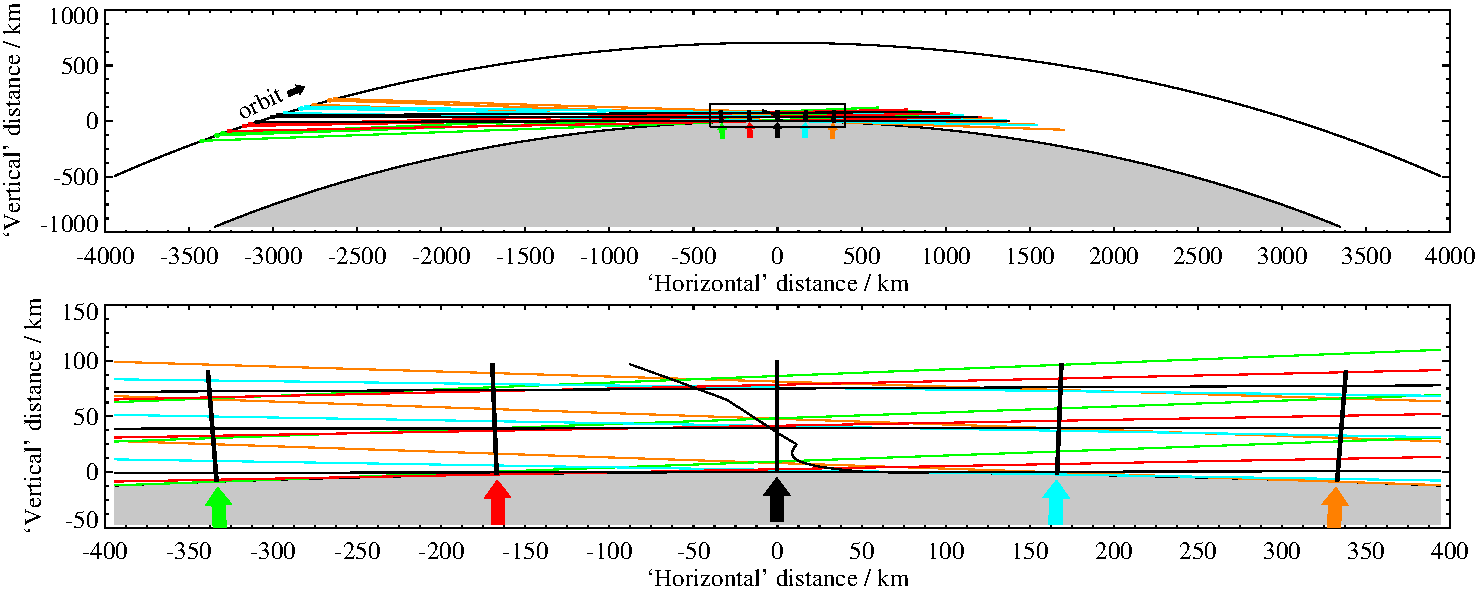
\includegraphics[width=\linewidth]{figures/geometry}
\caption{The top diagram shows a section of one orbit.  Three of the 120 limb
  ray paths per scan are indicated by the ``horizontal'' lines.  The lower
  diagram shows an expansion of the boxed region above.  The straight
  radial lines denote the location of the retrieved atmospheric
  profiles.  The limb ray scan closest to each profile is that whose
  color is the same as that of the arrow underneath.  The thin black
  line under the central profile indicates the locus of the limb tangent
  point for this scan, including the effects of refraction.}
\label{fig:Geometry}
\end{figure}

The Level~2 algorithms implement a standard \emph{Optimal Estimation}
retrieval approach \citep{Rodgers76,Rodgers00} that seeks the ``best''
value for the state vector (the profiles of temperature and abundances)
based on an optimal combination of the fit to the MLS radiance
observations, \emph{a priori} estimates of the state vector (from
climatological information and, for temperature in the troposphere and
lower stratosphere, analysis fields), and constraints on the smoothness
of the result.  This fit must often be arrived at in an iterative manner
because of the non-linear nature of the Aura MLS measurement system.

An innovative aspect of the retrieval algorithms for Aura MLS arises from
taking advantage of the fact that the MLS instrument looks in the
forward direction from the spacecraft.  Figure~\ref{fig:Geometry}
reviews the Aura MLS measurement geometry and shows that each radiance
observation is influenced by the state of the atmosphere for several
consecutive profiles.  In the \thisv Level~2 algorithms, the state vector
consists of ``chunks'' of several profiles of atmospheric temperature and
composition, which are then simultaneously retrieved from radiances
measured in a similar number of MLS scans.  Results from these ``chunks''
are then joined together to produce the products at a granularity of one
day (the chunks overlap in order to avoid ``edge effects'').

The retrieval state vector consists of vertical profiles of temperature
and composition on fixed pressure surfaces.  Between these fixed
surfaces, the forward models assume that species abundances and
temperature vary from surface to surface in a piecewise-linear fashion
(except for the abundance of H\cs2O, which is assumed to vary linearly in
the logarithm of the mixing ratio).  This has important implications for
the interpretation of the data as was described in
section~\ref{sec:BasisIssues}.  In addition to these profiles, the
pressure at the tangent point for the mid-point of each minor frame is
retrieved, based on both radiance observations and knowledge of tangent
point height from the MLS antenna position encoder and the Aura
spacecraft ephemeris and attitude determination.

Most of the MLS data products are deduced from observations of spectral
contrast, that is, variations in radiance as a function of frequency for
a given limb pointing.  Many of the systematic errors in the MLS
measurement system manifest themselves as a spectrally flat or slowly
spectrally varying error in radiance.  This is true of effects arising
both from the instrument (such as gain and offset during the limb scan)
and from the ``forward model'' (such as knowledge of continuum emission
and the impact of some approximations made in the forward model in order
to increase its speed).  In order to account for such effects, the
\thisv algorithms also retrieve spectrally flat (or slowly spectrally
varying) corrections to the MLS radiances, either in terms of an
additive radiance offset or an additive atmospheric extinction.

\section{The \texttt{Core}, \texttt{CorePlusR\emph{n}} approach}

\subsection{The need for separate ``phases''}

Many aspects of the MLS measurement system are linear in nature.  In
other words, there is a linear relationship between changes in aspects
of the atmospheric state and consequent changes in the MLS radiance
observations.  However, there are some components of the state vector
whose impact on the radiances is non-linear.  The most non-linear of
these is the estimate of the tangent pressure for each MIF of
observation.  The impact of water vapor in the upper troposphere on the
MLS radiance observations is also highly non-linear.  Solving for these
aspects of the state vector therefore requires several iterations.

The computational effort involved in retrieval and forward models scales
very rapidly (arguably as high as cubically) as a function of the size
of the measurement system (i.e., the number of elements in the state and
measurement vectors).  Thus it is desirable to simplify retrievals
involving strongly non-linear variables to a small subset of the
complete system, in order to cut down on the effort involved in
retrievals that require many iterations.

For this and other reasons, most retrieval algorithms are split into
\emph{phases}.  In the case of the MLS \thisv retrievals, there are many
such phases.  The first group of phases (collectively known as ``Core'')
use the 118\,GHz and 240\,GHz observations of O\cs2 and O\cp{18}O,
respectively, to establish estimates for temperature and tangent
pressure.  Upper tropospheric 190\,GHz radiances are used in these early
phases to establish a first order estimate of upper tropospheric
humidity.  The ``Core'' phases also include ``cloud screening''
computations (based on differences between observed and estimated
clear-sky radiances).  These identify minor frames where radiances in a
given radiometer have been subject to significant (and currently poorly
modeled) cloud scattering.  Such minor frames are ignored in \thisv
processing in certain radiometers.  Including information in such
cloud-contaminated conditions is a goal for future MLS data processing
versions.

The ``Core'', phases are followed by phases such as \texttt{CorePlusR3} and
\texttt{CorePlusR5}, where composition profiles are retrieved from a given
radiometer.  Sometimes (e.g., for \texttt{CorePlusR3}) these later phases
continue to retrieve temperature and pressure, continuing using
information from the 118\,GHz radiometers, as in ``Core''.  In other
phases (e.g., the \texttt{CorePlusR2} and \texttt{CorePlusR4} families of phases), the
118\,GHz information is neglected and temperature and pressure are
constrained to the results of ``Core''.  This choice is made based on
extensive testing aimed at maximizing the information yield from MLS
while minimizing the impact of inevitable systematic disagreements among
the different radiometers, introduced by uncertain spectroscopy and/or
calibration knowledge.

Table~\ref{tab:Phases} describes the phases in more detail.  Many
products (e.g.,\ ozone) are produced in more than one phase.  All the
separate measurements of these species are produced as diagnostic
quantities, and labeled according to the spectral region from which they
originated.  For example, the ozone obtained from the
\texttt{CorePlusR2} retrieval is known in the \thisv dataset as
\texttt{O3-190}.  In \thisv in order to reduce confusion for users of
MLS data, the algorithms also output ``standard products'', which is
typically a copy of one of the products from the
\texttt{CorePlusR\emph{n}} phases.  For example, the ``standard''
chlorine monoxide product is a copy of the \texttt{ClO-640} product.  In
the case of \thisv nitric acid, the standard product represents a hybrid
of the results from two phases.  Details of which standard product is
obtained from which phase are given in table~\ref{tab:StandardProducts}.

\newcommand{\mybox}[2]{\parbox[m]{#1}{\raggedright #2}}
\newcommand{\phase}[1]{\mybox{1.0in}{\texttt{#1}}}
\newcommand{\species}[1]{\mybox{2.2in}{#1}}
\newcommand{\measurements}[1]{\mybox{1.5in}{#1}}
\newcommand{\tablecomments}[1]{\mybox{3.6in}{#1}}

\begin{sidewaystable}
\renewcommand{\thempfootnote}{\sffamily[\arabic{mpfootnote}]}
\renewcommand{\arraystretch}{1.2}
\caption{The phases that form the \thisv retrieval
  algorithms.}  \vspace{1ex}
\label{tab:Phases}
\begin{minipage}{\linewidth}
\begin{center}\begin{small}\sffamily
\centering\begin{tabular}{llll}\toprule
\textbf{Phase} & \textbf{Target species}\footnote{\sffamily Tangent pressure and
    Geopotential height have been abbreviated to pTan (GHz/THz) and GPH
    respectively.  Minor state vector components such as ``baseline''
    and/or `extinction' have been omitted unless they are the specific
    focus of the phase.  Temperature, IWC, H\cs2O, RHi are ``high
    resolution''
    (12 surfaces per decade change in pressure from 1000\,hPa to 1\,hPa)
    unless otherwise stated. O\cs3 is low resolution except for the
    Core+R3 phase.} & \textbf{Measurements} &
\textbf{Comment} \\
\midrule
\flipfloprow
\phase{InitPTan} &
\species{T, pTan (GHz), GPH} & 
\measurements{R1A \& R1B~(118\,GHz)} & 
\tablecomments{Initial estimate of P/T, lower limit 261\,hPa} \\

\flipfloprow
\phase{InitR2} &
\species{H\cs2O, N\cs2O, CH\cs3CN, HCN, ClO, HNO\cs3, O\cs3, SO\cs2} &
\measurements{R2~(190\,GHz)} &
\tablecomments{Initial trace gas estimator, lower limit 100\,hPa} \\

\flipfloprow
\phase{R3InitRHi} &
\species{RHi, T\cs{cir}} &
\measurements{R3 (240\,GHz)} &
\tablecomments{Retrieves RHi profile from 316\,hPa and up, used mostly
  for ``near field'' cloud detection and to compute R3 T\cs{cir}} \\

\flipfloprow
\phase{CloudDetector} &
\species{none} &
\measurements{R3 (240\,GHz)} &
\tablecomments{Determines cloud screening for R2 (190\,GHz) and R3
  (240\,GHz)} \\

\flipfloprow
\phase{FinalPTan} &
\species{T, pTan~(GHz), GPH} & 
\measurements{R1A \& R1B~(118\,GHz), R3~(240\,GHz)} &
\tablecomments{Best P/T retrieval, lower limit 261\,hPa} \\ 

\flipfloprow
\phase{InitLowCloud} &
\species{T\cs{cir}} &
\measurements{All radiometers} &
\tablecomments{Determines cloud flags for all phases} \\

\flipfloprow
\phase{InitRHi} &
\species{UT RHi} &
\measurements{R2~(190\,GHz)} &
\tablecomments{Retrieve RHi in a \texttildelow6\,km-layer centered
  400\,--\,600\,hPa.  Uses only saturated radiances} \\ 

\flipfloprow
\phase{InitUTH} &
\species{Upper tropospheric H\cs2O} & 
\measurements{R2~(190\,GHz)} &
\tablecomments{Low vertical resolution (6/decade)} \\ 

\flipfloprow
\phase{CorePlusR3} & \species{T, pTan~(GHz), GPH, O\cs3\footnote{\sffamily On high vertical resolution
    grid}, CO, HNO\cs3, SO\cs2,
  RHi$^b$} &
\measurements{R1A \& R1B~(118\,GHz), R3~(240\,GHz)} &
\tablecomments{Retrievals down to 316\,hPa}\\ 

\flipfloprow
\phase{OzoneOnly} &
\species{O\cs3, CO} &
\measurements{R3~(240\,GHz)} &
\tablecomments{Retrievals down to 316\,hPa}\\ 

\flipfloprow
\phase{CorePlusR2} &
\species{H\cs2O, N\cs2O, HNO\cs3, ClO, O\cs3, HCN, CH\cs3CN, SO\cs2} &
\measurements{R1A \& R1B~(118\,GHz), R2~(190\,GHz)} & 
\tablecomments{H\cs2O retrieved down to 316\,hPa, other species 100\,hPa
(note no T, pTan, GPH retrieval)} \\ 

\flipfloprow
\phase{Hydrogen Cyanide} &
\species{HCN, O\cs3, HNO\cs3} &
\measurements{R2~(190\,GHz)} & 
\tablecomments{Retrievals down to 100\,hPa} \\ 

\flipfloprow
\phase{CorePlusR4AB14} & \species{ClO, BrO, HO\cs2, HOCl,
  HCl, O\cs3, HNO\cs3, CH\cs3CN, SO\cs2, CH\cs3Cl} &
\measurements{R4~(640\,GHz)} &
\tablecomments{Retrievals down to 147\,hPa}\\ 

\flipfloprow
\phase{Methanol} &
\species{CH\cs3OH, ClO, BrO, HO\cs2, HOCl, HNO\cs3, SO\cs2, CH\cs3Cl} &
\measurements{R2~(190\,GHz) and R4~(640\,GHz)} & 
\tablecomments{Retrievals down to 147\,hPa} \\ 

\flipfloprow
\phase{CorePlusR4AB13} & \species{HCl, O\cs3, SO\cs2} &
\measurements{R4~(640\,GHz)} &
\tablecomments{Retrievals down to 147\,hPa. This phase only performed when
  MLS band~13 is operating}\\ 

\flipfloprow
\phase{CorePlusR4B} & \species{N\cs2O, SO\cs2} &
\measurements{R4~(640\,GHz)} &
\tablecomments{Retrievals down to 147\,hPa}\\ 
\flipfloprow
\phase{HighCloud} &
\species{Cloud induced radiance, IWC, IWP} &
--- &
\tablecomments{Used for flagging clouds in Core+R3 and later phases and
  forms basis for cloud ice products.} \\ 

\flipfloprow
\phase{CorePlusR5} & \species{T, pTan~(GHz,~THz), GPH, OH, O\cs3} &
\measurements{R1A \& R1B~(118\,GHz), R5H and R5V~(2.5\,THz)} &
\tablecomments{Retrievals down to 68\,hPa (147\,hPa for Temperature)} \\
\bottomrule
\end{tabular}
\end{small}\end{center}
\end{minipage}
\end{sidewaystable}

\begin{table}
\sffamily
\renewcommand{\arraystretch}{1.3}
\caption{The origin of each of the ``standard products'' from
  \thisv.}
\vspace{1ex}
\label{tab:StandardProducts}
\centering\begin{tabular}{l>{\ttfamily}ll}\toprule
  \textbf{Product} & \sffamily\textbf{Origin} & \textbf{Spectral region}\\
  \midrule\flipfloprow
  BrO       & CorePlusR4AB14 & 640\,GHz \\
  \flipfloprow 
  CH\cs3Cl  & CorePlusR4AB14 & 640\,GHz \\
  \flipfloprow 
  CH\cs3CN  & CorePlusR4AB14 & 640\,GHz \\
  \flipfloprow 
  CH\cs3OH  & Methanol & 640\,GHz \\
  \flipfloprow 
  ClO       & CorePlusR4AB14 & 640\,GHz \\
  \flipfloprow 
  CO        & CorePlusR3 & 240\,GHz \\
  \flipfloprow 
  GPH       & CorePlusR3 & 118 \& 240\,GHz \\
  \flipfloprow 
  H\cs2O    & CorePlusR2 & 190\,GHz \\
  \flipfloprow 
  HCl       & CorePlusR4AB14 & 640\,GHz \\
  \flipfloprow 
  HCN       & HydrogenCyanide & 190\,GHz \\ 
  \flipfloprow 
  HNO\cs3   & \mybox{6cm}{CorePlusR2 \textsf{(15\,hPa and less)} \\ CorePlusR3 \textsf{(larger
    than 15\,hPa)}} &
  \mybox{2.5cm}{190\,GHz\\240\,GHz} \\
  \flipfloprow 
  HO\cs2    & CorePlusR4AB14 & 640\,GHz \\
  \flipfloprow 
  HOCl      & CorePlusR4AB14 & 640\,GHz \\
  \flipfloprow 
  IWC       & HighCloud & 240\,GHz \\
  \flipfloprow 
  IWP       & HighCloud & 240\,GHz \\
  \flipfloprow 
  N\cs2O    & CorePlusR2& 190\,GHz \\ 
  \flipfloprow 
  O\cs3     & OzoneOnly & 240\,GHz \\
  \flipfloprow 
  OH        & CorePlusR5 & 2.5\,THz \\
  \flipfloprow 
  RHi       & \mybox{6cm}{\sffamily\raggedright Computed from Temperature and H\cs2O} & 190\,GHz \\
  \flipfloprow 
  SO\cs2    & CorePlusR3 & 240\,GHz \\
  \flipfloprow 
  Temperature & CorePlusR3 & 118 \& 240\,GHz \\
  \bottomrule
\end{tabular}
\end{table}

\section{Forward models used in \thisv}

The retrieval algorithms in \thisv make use of a variety of different
forward models.  The most accurate is the so-called ``full'' forward
model described in \citet{EOSMLSFWMATBD} and
\citet{EOSMLSPolarizedFWMATBD}.  This is a hybrid line-by-line and
channel averaged model that computes radiances on appropriate grids of
frequency and tangent pressure that are then convolved with the MLS
frequency and angular responses.

This model is generally very time consuming, although for some
comparatively ``clean'' spectral regions the computational burden is small
enough that the full forward model can be used in the operational
retrievals.  In the \thisv retrieval algorithms, its use is restricted
mainly to radiance channels whose focus is the upper troposphere and
lower stratosphere, as these radiances generally have a non-linear
relationship to the state vector.

For many of the MLS channels, a simpler ``Linearized'' forward model can
be used.  This model invokes a simple first-order Taylor series to
estimate radiances as a function of the deviation of the state from one
of several pre-selected representative states.  The inputs to this model
are pre-computed radiances and derivatives corresponding to the
pre-selected states, generated by ``off-line'' runs of the full forward
model.

This model is by its nature approximate, and its use is generally
confined to the upper stratosphere and mesosphere where retrievals are
more linear in nature.  In addition, a ``cloud'' forward model can be
invoked to model the effects of scattering from cloud particles in the
troposphere and lower stratosphere \citep{EOSMLSCloudATBD}.  This model
was used in the simulation of radiances based on known model atmospheres
for the \thisv testing, but is not invoked in the \thisv retrieval
algorithms (the handling of clouds is described in more detail in
section~\ref{sec:Clouds}).

\section{The handling of clouds in \thisv}
\label{sec:Clouds}
\newcommand{\Tcir}{\ensuremath{T_\text{cir}}}

Thin clouds and atmospheric aerosols do not affect MLS atmospheric
composition measurements as the typical particle sizes are much smaller
than the wavelengths of the radiation being observed. The MLS \thisv
algorithms can reliably retrieve composition in moderately cloudy cases
(having small limb radiance perturbations) and in the case of the
Core+R3 retrieval this is handled by retrieving a frequency squared
dependent extinction (including background atmospheric absorption from
N\cs2, H\cs2O and unknown emitters).  In the other retrieval phases, by
contrast, a spectrally-flat baseline is used.  Thick clouds can affect
the MLS radiances beyond the modeling capability of this approach,
mainly through scattering processes.  Such situations and the affected
radiances are excluded from the retrievals, or their influence
down-weighted.

The first aspect of handling clouds in \thisv is therefore the flagging
of radiances that are believed to be significantly contaminated by cloud
effects.  To determine if a cloud is present in each MLS radiance
measurement, we estimate the so-called cloud-induced radiance (\Tcir).
This is defined as the difference between the measured radiance and the
radiance from a forward model calculation assuming clear-sky conditions.
Specific window channels (those that are most transparent deepest into
the atmosphere) in each radiometer are chosen to set these flags.

Cloud screening in the Core+R2 and Core+R3 phases is based on
determining the highest altitude limb view contaminated by cloud signals
and either rejecting all radiances below that altitude or, in the case
of less impacted channels, inflating their estimated radiance
precisions.  Clouds are detected by a combination of a radiance fit
$\chi^2$ quantity from Band~8 (240\,GHz isotopic oxygen line) retrieval
of temperature and pointing, and a cloud induced radiance calculation,
also using 240\,GHz measurements.  Cloud radiance scattering causes
severe line shape distortions which are most reliably detectable in the
Band~8 O\cp{18}O line fit, based on extrapolating a tangent pressure
estimate into the upper troposphere from the pressure information
obtained from the 118\,GHz Band~1 measurements (unaffected by clouds).
RHi from a previous phase is used to compute a cloud induced radiance
(T\cs{cir}).  The vertical profiles of $\chi^2$ and T\cs{cir} are
analyzed to find the highest limb view affected by cloud scattering, and
radiances below are handled accordingly.

The other aspect of cloud handling in \thisv is the estimation of cloud
ice water content (IWC) and ice water path (IWP) products from the final
\Tcir\ computed by the retrieval in the \texttt{HighCloud} phase.  More
information on these products and their derivation is given in
section~\ref{sec:StandardIWC}.

\begin{table}
\sffamily\mathversion{sans}
\renewcommand{\arraystretch}{1.4}
\caption{MLS frequency channels and thresholds for cloud flag}
\vspace{1ex}
\label{tab:CloudThresholds}
\centering\small\begin{tabular}{>{\ttfamily}l>{\ttfamily}llll}
\toprule
\sffamily\textbf{Radiometer} & \sffamily\textbf{Cloud channel} & \textbf{USB/LSB frequency
  / GHz} & 
\textbf{Low threshold} & \textbf{High threshold} \\
\midrule
%
\flipfloprow
R1[A/B]:118 & B[32/34]W:PT.C4 & 115.3 (LSB only) & $\mathsf{\Tcir <
-4}$\,K & none \\
%
\flipfloprow
R2:190 & B5F:ClO.C1 & 178.8 / 204.9 & $\mathsf{\Tcir <
-20}$\,K & $\mathsf{\Tcir > 10}$\,K \\
%
\flipfloprow
R3:240 & B8F:PT & 233.4\,--\,234.5 / 244.8\,--\,245.9 & none &
$\mathsf{\chi^2>30}$ \\
%
\flipfloprow
R4:640 & B11F:BrO.C23 & 635.9 / 649.8 & $\mathsf{\Tcir < -10}$\,K & none \\
\bottomrule
\end{tabular}
\end{table}

\section{The quantification of systematic uncertainty in MLS Level~2
  data}
\label{sec:SystematicUncertainty}

A major component of the validation of MLS data is the quantification of
the various sources of systematic uncertainty.  These can arise from
instrumental issues (e.g., radiometric calibration, field of view
characterization), spectroscopic uncertainty, and through approximations
in the retrieval formulation and implementation.  A comprehensive
quantification of these uncertainties was undertaken for the earlier
v2.2 MLS data and the results for each product reported in the relevant
validation papers (see the individual sections of
Chapter~\ref{chap:Results} for references). In many cases these accuracy
estimates are expected to apply for \thisv also.
Chapter~\ref{chap:Results} reports the expected accuracy for each
product, taken and/or modified from the v2.2 estimates as appropriate.

For each identified source of systematic uncertainty, its impact on MLS
measurements of radiance (or pointing where appropriate) has been
quantified and modeled.  These modeled impacts correspond to either
2-$\sigma$ estimates of uncertainties in the relevant parameter(s), or
an estimate of their maximum reasonable error(s) based on instrument
knowledge and/or design requirements.

For most of the uncertainty sources, the impact on MLS standard products
has been quantified by running perturbed radiances through the MLS data
processing algorithms.  Other (typically smaller) uncertainty sources
have been quantified by simple perturbation calculations.

Although the term ``systematic uncertainty'' is often associated with
consistent biases and/or scaling errors, many sources of ``systematic''
error in the MLS measurement system give rise to additional scatter.
For example, an error in the O\cs3 spectroscopy, while being a bias on
the fundamental parameter, will have an impact on the retrievals of
species with weaker signals (e.g., CO) that is dependent on the amount
and morphology of atmospheric ozone.  The extent to which such terms can
be expected to average down is estimated to first order by these ``full
up studies'' through their separate consideration of the bias and scatter
each uncertainty source introduces.

The results of these studies are summarized as ``accuracy'' (and in some
cases additional contributions to ``precision'') on a product by product
basis in the next chapter.  More details on the quantification for each
product are given in the MLS validation papers.  In addition Appendix~A
of \citet{ReadEtal07} gives more specific details of the perturbations
used in the study.

\section{A brief note on the \texttt{Quality} field}

As described in section~\ref{sec:StatusQuality}, the \texttt{Quality}
field in the \texttt{L2GP} files gives a measure of the fit achieved
between the observed MLS radiances and those computed by the forward
model given the retrieved MLS profiles.  \texttt{Quality} is computed
from a $\chi^2$ statistic for all the radiances considered to have
significantly affected the retrieved species (i.e., those close to the
relevant spectral lines), normalized by dividing by the number of
radiances.  \texttt{Quality} is simply the reciprocal of this statistic
(i.e., low values indicate large $\chi^2$, i.e., poor fits).

Ideally, the typical values of these normalized $\chi^2$ statistics will
be around one, indicating that radiances are typically fitted to around
their noise levels.  \texttt{Quality} will therefore also ideally have a
typical value of one.  For some species, however, because of uncertain
knowledge of spectroscopy and/or instrument calibration, the \thisv
algorithms are known to be consistently unable to fit some observed
radiances to within their predicted noise.  In many of these cases, the
noise reported on the radiances has been ``inflated'' to allow the
retrieval more leeway in fitting to radiances known to be challenging.
As the noise level is the denominator in the $\chi^2$ statistic, these
species will have typical $\chi^2$ statistics that are less than one and
thus typical values of \texttt{Quality} higher than one.  Accordingly,
differences in \texttt{Quality} from one species to another do not
reflect the species' relative validity, nor do version-to-version
increases in \texttt{Quality} for a given product necessarily indicate
improvements (or vice versa)

%%% Local Variables: 
%%% mode: latex
%%% TeX-master: "v4-x-report"
%%% End: 
 \chapter{Product-specific information}
%%\rcsInfo $Id: chapResults.tex,v 1.5 2015/02/11 06:03:21 livesey Exp $
\label{chap:Results}


\section{Overview of species-specific discussion}

This section describes each MLS \thisv ``standard product'' in more
detail.  An overview is given of the expected resolution, precision and
accuracy of the data.  The resolution is characterized by the averaging
kernels described below.  Precision is quantified through a combination
of the precision estimated by the MLS \thisv algorithms, through
reference to the systematic uncertainty budget described in
section~\ref{sec:SystematicUncertainty}, and through study of the actual
MLS data (e.g., consideration of the observed scatter in regions where
little natural variability is anticipated).

The systematic uncertainty reported is generally based on the study
described in section~\ref{sec:SystematicUncertainty}.  However, in some
cases larger disagreements are seen between MLS and correlative
observations than these quantifications would imply.  In such cases
(e.g., MLS 215\,hPa CO) the uncertainty quoted reflects these disagreements.

\subsection*{A note on the averaging kernel plots}

The averaging kernels shown in this section describe both the horizontal
(along track) and vertical (pressure) resolution of the MLS \thisv data.
While the averaging kernels vary somewhat from profile to profile, their
variation is sufficiently small that these samples can be considered
representative for all profiles.  The averaging kernel plots are
accompanied by estimates of the horizontal and vertical resolution of
the product defined by the full width at half maximum of the kernels.
Each kernel plot also shows the integrated areas under the kernels.

\speciestitle{Bromine monoxide}{BrO}{BrO}{%
\item[Useful range: ] 10\,--\,3.2\,hPa (day/night differences needed)
\item[Contact:] Luis Millan, \email{Luis.F.Millan@jpl.nasa.gov}}
\subsection*{Introduction}

The standard product for BrO is taken from the 640-GHz \texttt{CoreR4AB13}
retrieval. The spectral signature of BrO in the MLS radiances is very
small, leading to a very poor signal-to-noise ratio on individual MLS
observations.  Significant averaging (e.g., monthly zonal means) is
required to obtain scientifically useful results.  Large biases of
between 5 to 30\,pptv (typical BrO abundances range from 5 to 15\,pptv)
are seen in the data. These biases can be minimized by taking day/night
differences. For pressures of 4.6 hPa and greater, nighttime BrO is
negligible; however, for smaller pressures, nighttime BrO needs to be
taken into account. Table~\ref{tab:BrOSummary} summarizes the precision,
accuracy, and resolution of the MLS \thisv BrO product. The accuracy
assessment is based on v2.2 data, as described in the validation paper
\citep{KovalenkoEtal07}.

Note, the \thisv ``standard'' BrO product (as with earlier versions)
contain systematic biases and horizontal oscillations that present a
larger challenge than for other species.  Those interested in using MLS
BrO in scientific studies are strongly advised to contact the MLS team
before embarking on their research.  Different algorithms for BrO have
been developed by the MLS team, aimed at ameliorating some of these
artifacts \citep{MillanEtal12}, and those products (currently based on
\prevv input data) are being made available at the GSFC DISC\@.  The
product short name is ``\texttt{ML3DZMBRO}'' and it is available from:
\newcommand{\myus}{\rule{1ex}{0.8pt}}
\href{ftp://acdisc.gsfc.nasa.gov/data/s4pa/Aura_MLS_Level3/ML3DZMBRO.003/}%
{\texttt{ftp://acdisc.gsfc.nasa.gov/data/s4pa/Aura\_MLS\_Level3/ML3DZMBRO.003/}}

\subsection*{Vertical Resolution}
\oneverticalavk{BrO}{BrO}

Figure~\ref{fig:AvkBrO} shows that the vertical resolution for the \thisv
MLS BrO is about 5.5\,km in the 10 to 4.6\,hPa pressure region, 
degrading to 6\,km at 3.2\,hPa.

\subsection*{Precision}

\begin{figure}
\begin{center}
  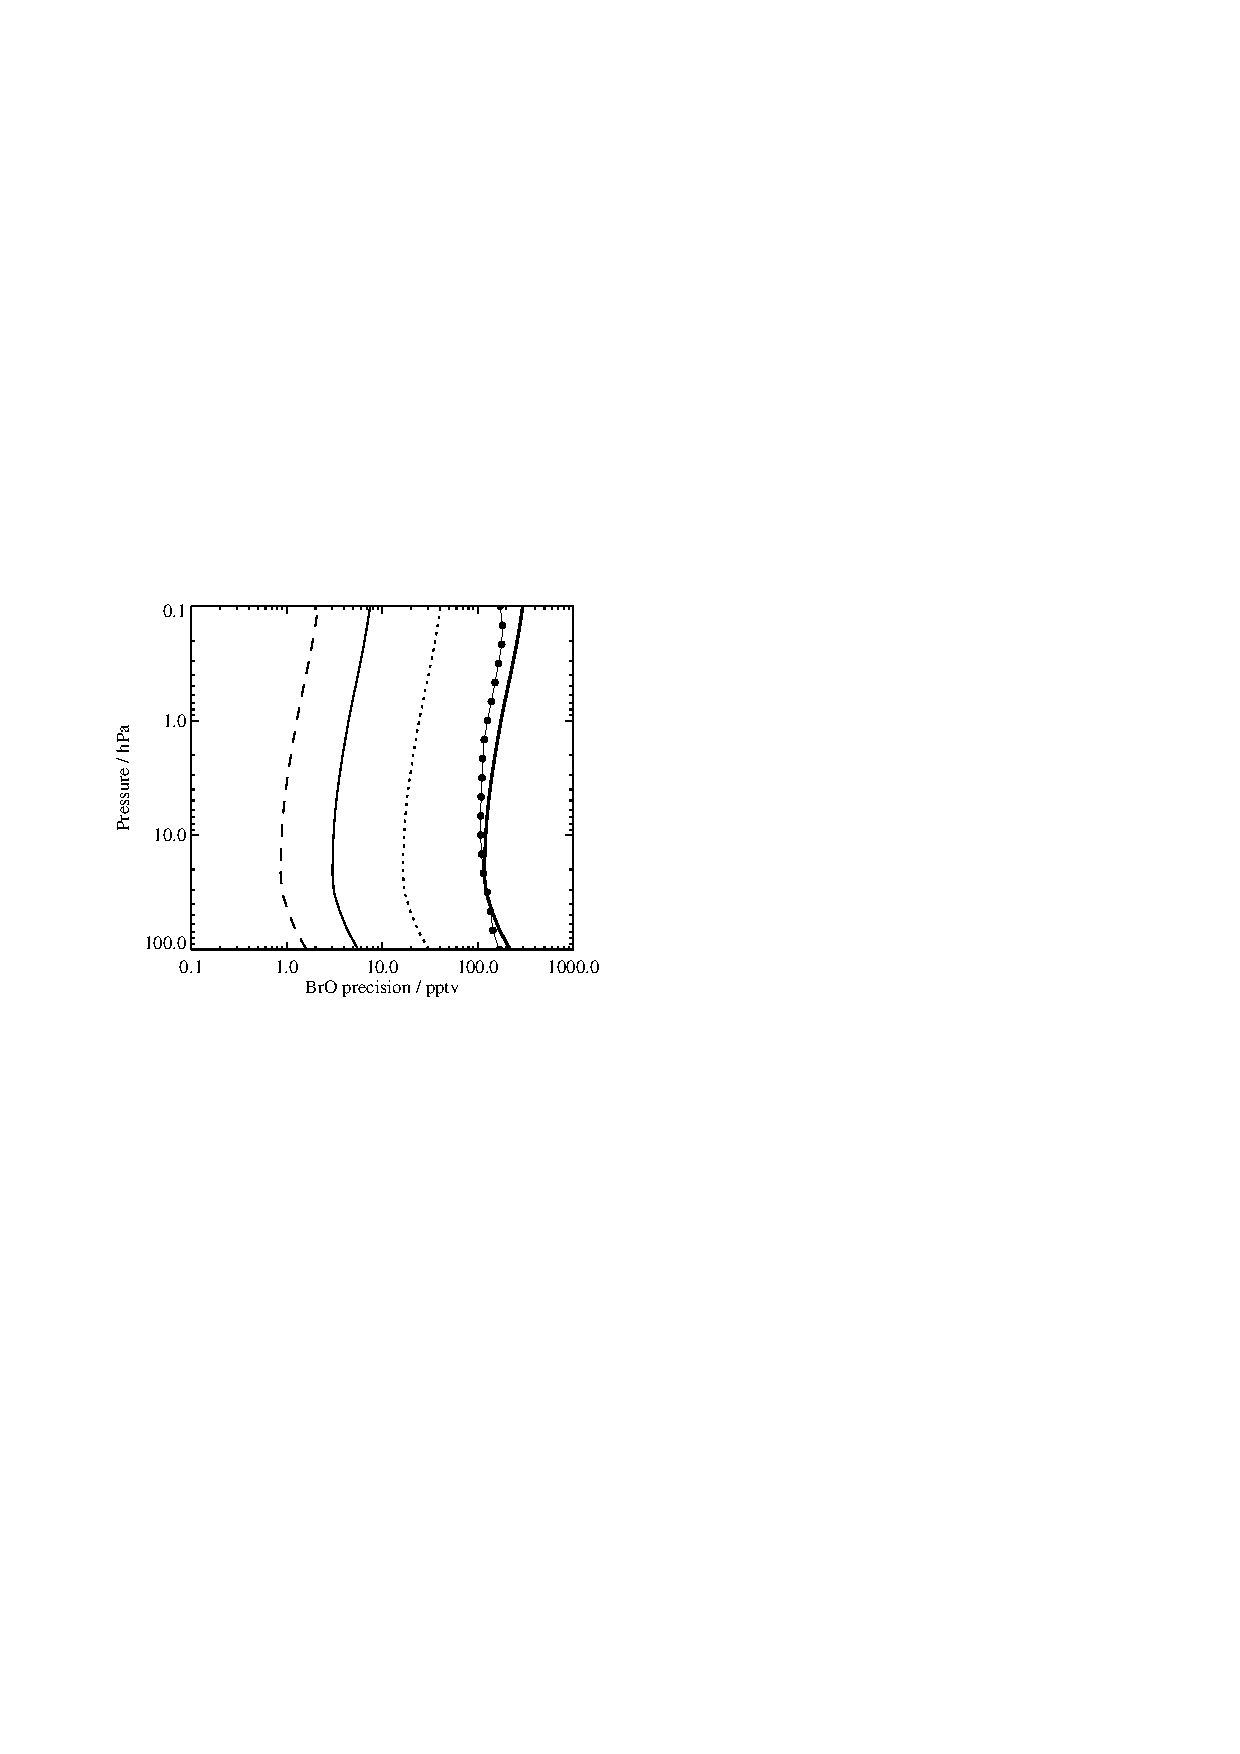
\includegraphics[width=0.4\linewidth]{figures/bro-precision}
\end{center}
\caption{Comparison of the MLS \thisv BrO precision as estimated from
  scatter in the retrieved data (circles) with that expected from the
  retrieval (thick line), for a single profile.  Also shown is the
  expected precision for the day/night difference of 10\degsym\ zonal
  mean profiles averaged over a day (dotted line), a month (thin line)
  and a year (dashed line).}
\label{fig:BrOPrecision}
\end{figure}

The expected precision in a retrieved profile is calculated from
radiance noise and reported for each retrieved data point.  The value of
the expected precision is flagged negative or zero if it is worse than
50\% of the value of the a priori precision.
Figure~\ref{fig:BrOPrecision} compares the expected precision (thick
line) on an individual MLS BrO measurement with that deduced from
observations of scatter in night-time observations (expected to be
zero). Also shown are the expected precisions for daily, monthly, and
yearly 10\degsym\ zonal means. For the minimal averaging recommended, a
monthly 10\degsym\ zonal mean, which corresponds to about 3,000
measurements, the precision is about $\pm$4\,ppt. See
Table~\ref{tab:BrOSummary} for more details.

\subsection*{Accuracy}

The accuracy of the MLS BrO product is summarized in
Table~\ref{tab:BrOSummary}. The effect of each identified source of
systematic error on MLS measurements of radiance has been quantified and
modeled \citep{ReadEtal07}. These quantified effects correspond to
either $2\sigma$ estimates of uncertainties in each MLS product, or an
estimate of the maximum reasonable uncertainty based on instrument
knowledge and/or design requirements. More discussion is given in
\cite{KovalenkoEtal07}.  While that paper described v2.2 BrO, findings
are expected to be applicable also to \thisv. The potential additive bias
in MLS BrO measurements can be as high as about $\pm$30\,ppt
(\texttildelow400\%) at 10\,hPa, decreasing to about $\pm$6\,pptv (50\%) at
3.2\,hPa. The potential scaling uncertainty over the pressure range of
10 to 3.2\,hPa is about $\pm$20\%. The additive bias is dramatically
reduced by subtracting the nighttime signal from the daytime signal.
Taking day/night differences does not affect the scaling uncertainty,
which remains at about $\pm$20\%. If the MLS BrO data is used at 3.2 hP,
the day/night difference value will need to be adjusted to compensate
for the non-negligible nighttime BrO. We note that this method of taking
day/night differences is not applicable for polar summer and winter
during periods of continuous sunlight or darkness.

\subsection*{Data screening}
\label{sec:BrOScreening}
\begin{description}
\item[Pressure range:] \screeningrule{10\,--\,3.2 hPa} \standardrangestatement
\item[Averaging required:] \screeningrule{Significant averaging (such as
    monthly zonal means) is required if useful scientific data are
    sought.}
\item[Diurnal differences:] \screeningrule{For use in any scientific
    study, day / night or ascending / descending differences should be used
    to alleviate biases.}  Note that, for 3.2\,hPa, the non-zero
  nighttime expected abundances BrO needs to be taken into account.
  \standardprecisionrule \evenstatusrule
\item[Clouds:] \cloudsokrule
\item[Quality:] \qualityrule{1.3}
\item[Convergence:] \convergencerule{1.05}
\end{description}

\subsection*{Artifacts}
Significant additive biases are seen in the BrO data, as discussed
above. Day / night (or ascending / descending) differences must be used to
reduce these.  For 3.2 hPa, nighttime BrO needs to be taken into
account \citep{KovalenkoEtal07}.

A systematic horizontal (i.e., profile-to-profile) oscillation has been
discovered in MLS \thisv (and earlier) standard BrO product.  This
presents a significant challenge to the interpretation of the BrO
observations.  Users are strongly advised to contact the MLS team before
embarking on research involving the MLS standard BrO product.  As
described above, use of other BrO products is preferable to using the
Level~2 BrO data.

\subsection*{Review of comparisons with other data sets}
We have calculated total bromine, Br$_{y}$, from MLS measurements of BrO
using a photochemical model, and compared this with Br$_{y}$ similarly
inferred from balloon-borne measurements of BrO, good agreement is seen
\citep{KovalenkoEtal07}.

\begin{table}
\caption{Summary of the Aura MLS \thisv BrO product.}
\vspace{\tablecaptionsep}
\label{tab:BrOSummary}
\begin{minipage}{\linewidth}
\centering\begin{tabular}{cccccl}
\toprule
\parbox[m]{5em}{\bfseries\centering Pressure range} &
\parbox[m]{4em}{\bfseries\centering Vertical res. / km} &
\parbox[m]{4.5em}{\bfseries\centering Precision\footnote{The precision quoted is for a 10\degsym\
    monthly zonal mean} / pptv} &
\parbox[m]{4.5em}{\bfseries\centering Bias uncertainty\footnote{Because of large biases in
    the data, the daytime and nighttime BrO data are unsuitable for
    scientific use, so day/night differences must be used. Note that
    day/night differences are not useful for polar winter and summer,
     where BrO does not undergo a diurnal variation.} / pptv} &
\parbox[m]{5em}{\bfseries\centering Scaling uncertainty\footnote{Based on modeled impacts
    of systematic errors} / \%} &
\textbf{Comments} \\
\midrule
%
2.2\,hPa and less & -- & -- & -- & -- & Unsuitable for scientific use
  \\ \addlinespace[2ex]
%
3.2\,hPa & 6 & $\pm$5 &$\pm$6 & $\pm$20
& \parbox[m]{10em}{\raggedright Need to
account for non-negligible night time BrO} \\ \addlinespace[2ex]
%
4.6 & 5.5 & $\pm$4 & $\pm$9  & $\pm$20 \\
6.8 & 5.5 & $\pm$4 & $\pm$20 & $\pm$20 \\ 
10  & 5.5 & $\pm$4 & $\pm$30 & $\pm$20 \\ 
150\,--\,15\,hPa   & -- & -- & -- & -- & Unsuitable for scientific use \\
1000\,--\,215\,hPa & -- & -- & -- & -- & Not retrieved \\
\bottomrule
\end{tabular}
\end{minipage}
\end{table}

%%% Local Variables: 
%%% mode: latex
%%% TeX-master: "v4-x-report"
%%% End: 
 \speciestitle{Methyl chloride}{CH\cs3Cl}{CH3Cl}%
{\item[Useful range:] 147\,--\,4.6\,hPa
\item[Contact:] Michelle Santee, \email{Michelle.L.Santee@jpl.nasa.gov}}

\subsection*{Introduction}

The v2.2 MLS ClO measurements were characterized by a substantial
(\texttildelow0.1\,--\,0.4\,ppbv) negative bias at retrieval levels
below (i.e., pressures larger than) 22\,hPa.  \citet{SanteeEtal08clo}
suggested that contamination from an interfering species such as
CH\cs3Cl, which has lines in two wing channels of the \mbox{640-GHz}
band used to measure ClO, could have given rise to the bias; they
showed results from early v3 algorithms in which CH\cs3Cl was also
retrieved that demonstrated significant reduction in the bias in lower
stratospheric ClO\@.  Further refinements in the \prevv algorithms
yielded not only an improved ClO product, but also a reliable
retrieval of CH\cs3Cl.  The quality and reliability of the \prevv MLS
CH\cs3Cl measurements were assessed in detail by
\citet{SanteeEtal13}.

As for ClO, the standard CH\cs3Cl product is derived from radiances
measured by the radiometer centered near 640\,GHz. The MLS \thisv CH\cs3Cl
data are scientifically useful over the range 147 to 4.6\,hPa.  A summary
of the precision and resolution (vertical and horizontal) of the \thisv
CH\cs3Cl measurements as a function of altitude is given in
Table~\ref{tab:CH3ClSummary}.  More details on the quality of the MLS
\thisv CH\cs3Cl measurements are given below.

\subsection*{Differences between \prevvSlash and \thisv}

\begin{figure}
\begin{tabular}{@{}l@{}l@{}}
\includegraphics[angle=90,width=0.5\linewidth]{figures/InspectZMContour_CH3Cl--v4-1_CH3Cl--v3-3_2009m07_LatPress-All-noScreen-panel1}&
\includegraphics[angle=90,width=0.5\linewidth]{figures/InspectZMContour_CH3Cl--v4-1_CH3Cl--v3-3_2009m07_LatPress-All-noScreen-panel2}\\
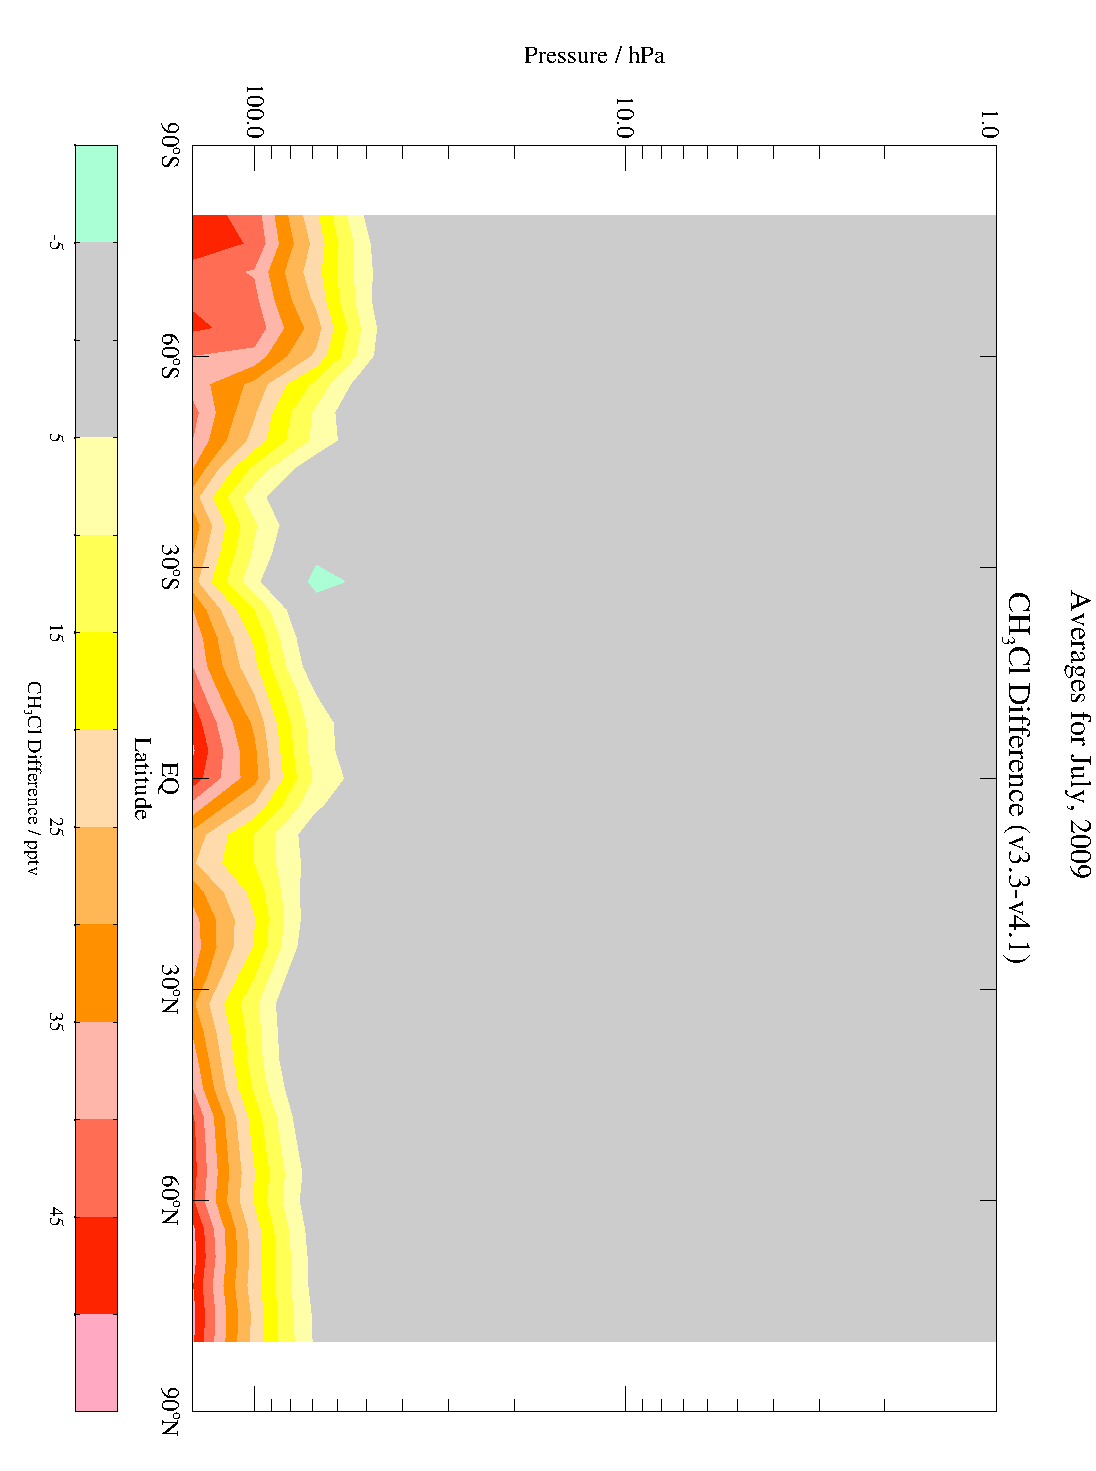
\includegraphics[angle=90,width=0.5\linewidth]{figures/InspectZMContour_CH3Cl--v4-1_CH3Cl--v3-3_2009m07_LatPress-All-noScreen-panel3}&
\raisebox{2cm}{\parbox[b]{0.5\textwidth}{%
\caption{Zonal averages of MLS CH\cs3Cl profiles for a representative
  month (July 2009), showing the MLS \thisv mixing ratios (upper left), the
  \prevv mixing ratios (upper right), and their differences in pptv (\prevv
  minus \thisv, lower left) as a function of pressure.\label{fig:zmcontourCH3Cl}}}}%
\end{tabular}
\end{figure}

Changes in CH\cs3Cl between \thisv and \prevvSlash result from
modifications to upstream retrievals of tangent pressure etc., and small
updates to the spectroscopy database for some molecules.  Differences in
the retrieved CH\cs3Cl abundances between the two versions range from
less than 10\,pptv at 68\,hPa and lower pressures to
\texttildelow50\,pptv at 147\,hPa (Figure~\ref{fig:zmcontourCH3Cl}), or
typically within $\pm$10\%, with \thisv mixing ratios generally smaller.

\subsection*{Resolution}
\onestandardavk{CH3Cl}{CH\cs3Cl}%

The resolution of the retrieved data can be described using
``averaging kernels'' \citep[e.g.,][]{Rodgers00}; the two-dimensional
nature of the MLS data processing system means that the kernels
describe both vertical and horizontal resolution.  Values of the
integrated kernel near unity indicate that the majority of information
for that level has come from the measurements themselves and not the a
priori; Figure~\ref{fig:AvkCH3Cl} shows that the measurements dominate
at pressures greater than 3.2\,hPa, above which level the integrated
kernel drops below 0.5. Smoothing, imposed on the retrieval system in
both the vertical and horizontal directions to enhance retrieval
stability and precision, degrades the inherent resolution of the
measurements.  Thus, although CH\cs3Cl measurements are reported at
six pressure levels per decade change in pressure (spacing of
\texttildelow2.7\,km), the vertical resolution of the \thisv
CH\cs3Cl data as determined from the full width at half maximum of the
rows of the averaging kernel matrix shown in Figure~\ref{fig:AvkCH3Cl}
is \texttildelow4\,--\,6\,km in most of the lower stratosphere,
degrading to \texttildelow8\,--\,10\,km at and above (i.e., at
pressures less than) 15\,hPa.  The averaging kernels are fairly
symmetric, and for the most part they peak at their nominal position.
However, overlap in the averaging kernels for the 100 and 147\,hPa
retrieval surfaces indicates that the 147\,hPa retrieval does not
provide as much independent information as is given by retrievals at
higher altitudes.  Figure~\ref{fig:AvkCH3Cl} also shows horizontal
averaging kernels, from which the along-track horizontal resolution is
determined to be \texttildelow600\,km at 147\,hPa,
\texttildelow450\,--\,500\,km from 100 to 22\,hPa, and
\texttildelow550\,--\,850\,km at and above 15\,hPa.  The cross-track
resolution, set by the width of the field of view of the
\mbox{640-GHz} radiometer, is \texttildelow3\,km.  The along-track
separation between adjacent retrieved profiles is 1.5\degsym\ great
circle angle (\texttildelow165\,km), whereas the longitudinal
separation of MLS measurements, set by the Aura orbit, is
10\degsym--\,20\degsym\ over low and middle latitudes, with much finer
sampling in the polar regions.

\subsection*{Precision}

\begin{figure}
\centering\includegraphics[width=10.0cm]{figures/MLSascdsc_CH3Cl}
\caption{(left) Ensemble mean profiles for ascending (light red) and
  descending (dark red) orbit matching pairs of MLS \thisv CH\cs3Cl
  profiles averaged over a representative year of data (2009).
  Symbols indicate MLS retrieval pressure levels.  (right) Mean
  differences (ascending$-$descending) in pptv (green solid line).
  Also shown are the standard deviations about the mean differences
  (light blue solid line) and the root sum square (RSS) of the
  precisions calculated by the retrieval algorithm for the two sets of
  profiles (light blue dashed line). The observed scatter about the
  mean differences and the reported precision values have been scaled
  by $\mathsf{1/\sqrt{2}}$ (to convert from standard deviations of differences
  into standard deviations of individual data points); hence the light
  blue solid line represents the statistical repeatability of the MLS
  measurements, and the light blue dashed line represents the expected
  $1\sigma$ precision for a single profile.  The thin black
  lines mark zero in each panel.  The number of crossing pairs of
  measurements being compared at each pressure level is noted in the
  space between the panels.}
\label{fig:mlsascdscCH3Cl}
\end{figure}

The precision of the MLS CH\cs3Cl data is estimated empirically by
comparing profiles measured at the intersections of ascending (day)
and descending (night) portions of the orbit. Under ideal conditions
(i.e., a quiescent atmosphere), the standard deviation about the mean
differences between such matched profile pairs provides a measure of
the precision of the individual data points. In practice, however,
real changes in the atmosphere may occur over the 12\,h interval
between the intersecting measurement points, in which case the
observed scatter provides an upper limit on the estimate of precision,
assuming that the a priori has a negligible influence on the retrieval
(a reasonable assumption at least at pressures greater than
3.2\,hPa). The precision estimates were found to be essentially
invariant with time; results for a representative year of data are
shown in Figure~\ref{fig:mlsascdscCH3Cl}. The observed standard
deviation values are \texttildelow100\,pptv or less throughout the
vertical domain. Mean differences between paired crossing profiles are
\texttildelow10\,pptv or less except at the lowest two levels, where
they reach 20--25\,pptv. Given the large number of data points being
compared, these ascending$-$descending differences are substantially
larger than the standard error of the mean, implying the presence of
significant systematic biases. These biases likely arise from the
cumulative effect of various factors in the retrieval system that can
vary diurnally or along the orbit, such as interferences from
temperature or other atmospheric constituents (e.g., H\cs2O and ClO),
or thermal emissions from the MLS antenna.

The precision reported for each data point by the Level 2 data
processing system exceeds the observationally determined precision
throughout the vertical range (Figure~\ref{fig:mlsascdscCH3Cl}),
indicating that the vertical smoothing (regularization) applied to
stabilize the retrieval system and improve the precision has a
non-negligible influence. Because the reported precisions take into
account occasional variations in instrument performance, the best
estimate of the precision of an individual data point is the value
quoted for that point in the L2GP files, but it should be borne in
mind that this approach slightly overestimates the actual measurement
noise. The estimates reported here represent the precisions at each
pressure level of a single profile; precision can generally be
improved by averaging, with the precision of an average of $N$
profiles being 1/$\sqrt{N}$ times the precision of an individual
profile (although the actual standard error of the mean can in some
cases be even smaller \citep{TooheyAndVonClarmann13}).

\subsection*{Range}

Although CH\cs3Cl is retrieved over the range 147 to 0.001\,hPa,
because of the degradation in resolution and expected precision, the
reduction in independent information contributed by the measurements,
and the results of simulations using synthetic data as input radiances
to test the closure of the retrieval system, the data are not deemed
reliable at retrieval pressures less than 4.6\,hPa. Despite the
overlap in the averaging kernels for the 147 and 100\,hPa surfaces
discussed above, the simulations show that the retrieved CH\cs3Cl
values track the variations in the ``truth'' field at both levels.
Moreover, the retrievals (of real data) at 147\,hPa display
significant features not seen at 100\,hPa (not shown) that are
believed to represent actual atmospheric variations. Thus, we
recommend that the \thisv CH\cs3Cl data may be used for scientific
studies between 147 and 4.6\,hPa (inclusive), although the reduced
sensitivity at the extremes of this range, as well as the relatively
coarse vertical resolution of the retrieved profiles, should be borne
in mind.

\subsection*{Accuracy}

The effects of various sources of systematic uncertainty (e.g.,
instrumental issues, spectroscopic uncertainty, and approximations in
the retrieval formulation and implementation) on the MLS \prevv
CH\cs3Cl measurements were quantified through a comprehensive set of
retrieval simulations; see \citet{SanteeEtal13} for details of
how the analysis was conducted and the magnitude of the expected
biases and additional scatter each source of uncertainty may introduce
into the data.  In aggregate, systematic uncertainties were estimated
to induce in the \prevv CH\cs3Cl measurements biases of up to 45\% and
additional scatter of up to 25\% at and below (i.e., at pressures
greater than) 10\,hPa.  The total systematic uncertainty, calculated
by combining (RSS) the contributions from both the bias and the
scatter terms, is approximately 30--45\% in the upper troposphere /
lower stratosphere.  Uncertainties are expected to be of similar
magnitude in \thisv, but a comprehensive \thisv systematic error
analysis will be the subject of future work.

\subsection*{Review of comparisons with other datasets}

Extensive comparisons of MLS \prevv CH\cs3Cl data with a variety of
different platforms (balloon-borne, aircraft, and satellite instruments)
were presented by \citet{SanteeEtal13}.

\subsection*{Data screening}
\label{sec:CH3ClScreening}
\begin{description}
\item[Pressure range:]  \screeningrule{147\,--\,4.6\,hPa}

  \standardrangestatement
  
  \standardprecisionrule
  
\item[Status flag:] \screeningrule{Only use profiles for which the
  \texttt{Status} field is zero.}  

  We recommend that all profiles with nonzero values of
  \texttt{Status} be discarded, because of the potential impact of
  cloud artifacts at lower levels.  Note, however, that rejecting in
  their entirety all profiles with nonzero \texttt{Status} may be
  unnecessarily severe at and above (i.e., at pressures equal to or
  smaller than) 46\,hPa, where clouds have negligible impact; thus
  otherwise good-quality profiles with nonzero but even
  \texttt{Status} values may be used without restriction at those
  levels as long as they are removed at larger pressures.  See
  Section~\ref{sec:StatusQuality} for more information on the
  interpretation of the \texttt{Status} field.

\item[Quality:] \qualityrule{1.3}

  This threshold for \texttt{Quality} (unchanged from \prevv)
  typically excludes less than 1\% of CH\cs3Cl profiles on a daily
  basis; note that it potentially discards some ``good'' data points
  while not necessarily identifying all ``bad'' ones.

\item[Convergence:] \convergencerule{1.05}

  On a typical day this threshold for \texttt{Convergence} (unchanged
  from \prevv) discards very few (0.3\% or less) of the CH\cs3Cl
  profiles, most (but not all) of which are also filtered out by the
  other quality control measures.
\end{description}

\subsection*{Artifacts}

\begin{itemize}
\item Significant ascending$-$descending differences imply the
  presence of systematic biases at the bottom two retrieval pressure
  levels.  However, various analyses performed separately on sets of
  ascending-only and descending-only measurements suggest that,
  although significant, these biases will have little or no impact on
  most scientific conclusions based on the MLS CH\cs3Cl measurements.
\end{itemize}

\subsection*{Desired improvements for future data version(s)}

\begin{itemize}
\item Minimize the impact of thick clouds on the retrievals to further
  improve the CH\cs3Cl measurements in the upper troposphere and
  lowermost stratosphere.
\end{itemize}

\begin{table*}[bp]
\caption{Summary of Aura MLS \thisv CH\cs3Cl Characteristics}\vspace{0.5ex}
\label{tab:CH3ClSummary}
\begin{minipage}{\linewidth}
\renewcommand{\thefootnote}{\thempfootnote}
\centering\begin{tabular}{ccccl}
\toprule
\parbox[m]{18mm}{\bfseries\centering{Pressure\\ / hPa}} &
\parbox[m]{24mm}{\bfseries\centering{Resolution\\ V $\times$ H%
\footnote{Vertical and Horizontal resolution in along-track direction.} \\ / km}} &
\parbox[m]{18mm}{\bfseries\centering{Precision%
    \footnote{Precision on individual profiles.} \\/ pptv}} &
\parbox[m]{20mm}{\bfseries\centering{Accuracy\\ / \%}} &
\parbox[m]{40mm}{\bfseries\centering{Known Artifacts\\ or Other Comments}} \\
%
\midrule
%
3.2\,--\,0.001 & ---                             & ---      & ---    & Unsuitable for scientific use\\
%
15\,--\,4.6    & 8\,--\,10 $\times$ 550\,--\,850 & $\pm$100 & 30--75 & \\
%
100\,--\,22    & 4\,--\,6  $\times$ 450\,--\,500 & $\pm$100 & 30--45 &  \\
%
147            & 4         $\times$ 600          & $\pm$100 & 45     & \\
%
1000\,--\,215  & ---                             & ---      & ---    & Not retrieved\\
%
\bottomrule
\end{tabular}
\end{minipage}
\end{table*}

%%% Local Variables: 
%%% mode: latex
%%% TeX-master: "v4-x-report"
%%% End: 

 \speciestitle{Methyl cyanide}{CH\cs3CN}{CH3CN}{%
\item[Useful range:] 46\,--\,1.0\,hPa
\item[Contact:] Michelle Santee, \email{Michelle.L.Santee@jpl.nasa.gov}}

\subsection*{Introduction}

In \thisv, as in \prevv, the standard CH\cs3CN product is taken from
radiances measured by the radiometer centered near 640\,GHz.  The
CH\cs3CN retrieval is largely unchanged in \thisv. Neither the \prevv
nor the \thisv CH\cs3CN data have been validated extensively at the time
of writing; such validation is planned for the future.  However, the
\thisv CH\cs3CN data are deemed to be scientifically useful over the
range 46 to 1\,hPa, except in the winter polar regions, where they may
exhibit large biases below 10\,hPa.  Data retrieved at higher pressures
may be used with caution in certain circumstances.  A summary of the
estimated precision and resolution (vertical and horizontal) of the
\thisv CH\cs3CN measurements as a function of altitude is given in
Table~\ref{tab:CH3CNSummary}.

\subsection*{Differences between \prevvSlash and \thisv}

\begin{figure}
\begin{tabular}{@{}l@{}l@{}}
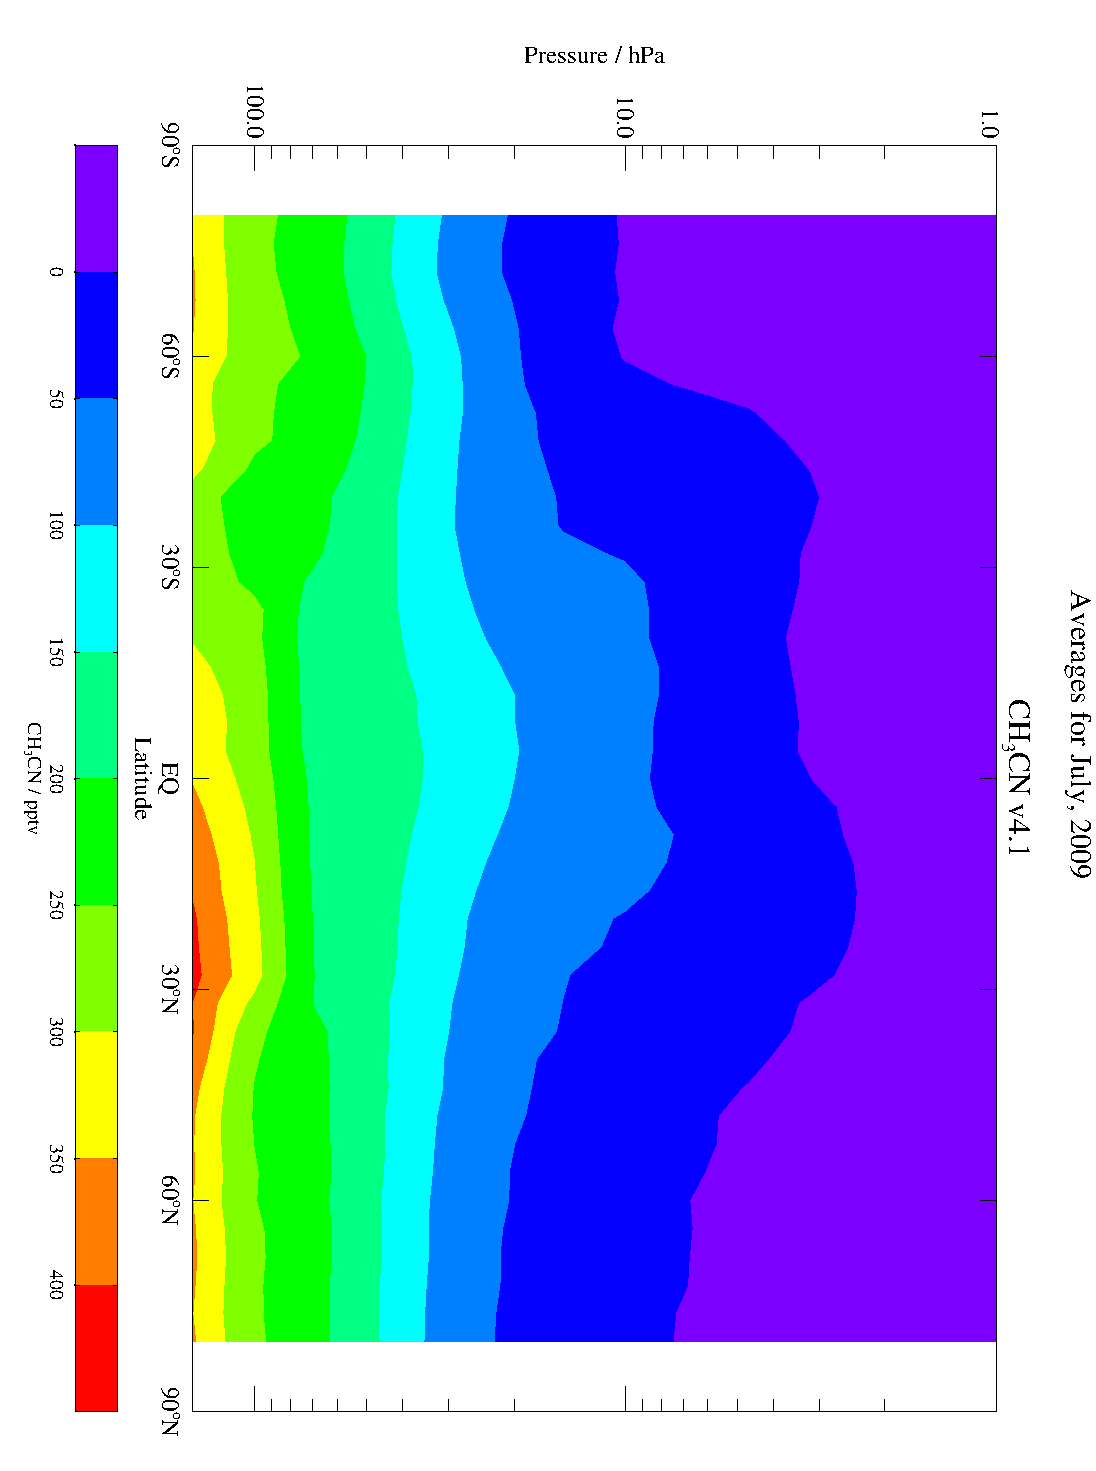
\includegraphics[angle=90,width=0.5\linewidth]{figures/InspectZMContour_CH3CN--v4-1_CH3CN--v3-3_2009m07_LatPress-All-noScreen-panel1}&
\includegraphics[angle=90,width=0.5\linewidth]{figures/InspectZMContour_CH3CN--v4-1_CH3CN--v3-3_2009m07_LatPress-All-noScreen-panel2}\\
\includegraphics[angle=90,width=0.5\linewidth]{figures/InspectZMContour_CH3CN--v4-1_CH3CN--v3-3_2009m07_LatPress-All-noScreen-panel3}&
\raisebox{2cm}{\parbox[b]{0.5\textwidth}{%
    \caption{Zonal averages of MLS CH\cs3CN profiles for a representative
      month (July 2009), showing the MLS \thisv mixing ratios (upper left), the
      \prevv mixing ratios (upper right), and their differences in pptv (\prevv
      minus \thisv, lower left) as a function of pressure.\label{fig:zmcontourCH3CN}}}}%
\end{tabular}
\end{figure}

Changes in CH\cs3CN between \thisv and \prevvSlash result from
modifications to upstream retrievals of tangent pressure etc., and small
updates to the spectroscopy database for some molecules.  Differences in
the retrieved CH\cs3CN abundances between the two versions are typically
less than 10\,pptv, but can reach 20\,pptv (still within $\pm$5\%) at
147\,hPa, particularly at higher latitudes
(Figure~\ref{fig:zmcontourCH3CN}).

\subsection*{Resolution}
\onestandardavk{CH3CN}{CH\cs3CN}%

The resolution of the retrieved data can be described using
``averaging kernels'' \citep[e.g.,][]{Rodgers00}; the two-dimensional
nature of the MLS data processing system means that the kernels
describe both vertical and horizontal resolution.  Values of the
integrated kernel near unity indicate that the majority of information
for that level has come from the measurements themselves and not the a
priori; Figure~\ref{fig:AvkCH3CN} shows that the measurements dominate
throughout most of the vertical range. Smoothing, imposed on the
retrieval system in both the vertical and horizontal directions to
enhance retrieval stability and precision, degrades the inherent
resolution of the measurements.  Thus, although CH\cs3CN measurements
are reported at six pressure levels per decade change in pressure
(spacing of \texttildelow2.7\,km), the vertical resolution of the
\thisv CH\cs3CN data as determined from the full width at half maximum
of the rows of the averaging kernel matrix shown in
Figure~\ref{fig:AvkCH3CN} degrades from 4\,km at 147\,hPa to
\texttildelow5\,--\,6\,km in the lower stratosphere, and then
further worsens to \texttildelow7\,--\,8\,km in the upper
stratosphere.  Substantial overlap in the averaging kernels for the
100 and 147\,hPa retrieval surfaces (which both peak at 100\,hPa)
indicates that the 147\,hPa retrieval does not provide as much
independent information as is given by retrievals at higher altitudes.
Figure~\ref{fig:AvkCH3CN} also shows horizontal averaging kernels,
from which the along-track horizontal resolution is determined to be
\texttildelow400\,--\,700\,km over most of the vertical range.  The
cross-track resolution, set by the width of the field of view of the
\mbox{640-GHz} radiometer, is \texttildelow3\,km.  The along-track
separation between adjacent retrieved profiles is 1.5\degsym\ great
circle angle (\texttildelow165\,km), whereas the longitudinal
separation of MLS measurements, set by the Aura orbit, is
10\degsym--\,20\degsym\ over low and middle latitudes, with much finer
sampling in the polar regions.

\subsection*{Precision}

\begin{figure}
\centering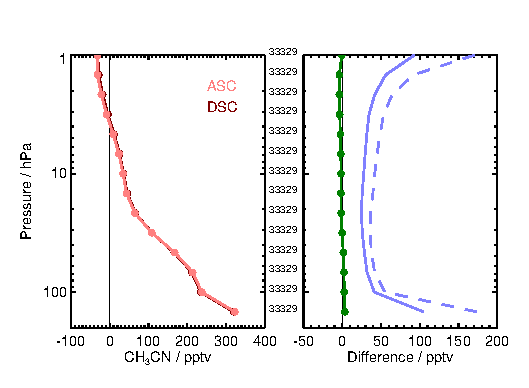
\includegraphics[width=10.0cm]{figures/MLSascdsc_CH3CN}
\caption{(left) Ensemble mean profiles for ascending (light red) and
  descending (dark red) orbit matching pairs of MLS \thisv CH\cs3CN
  profiles averaged over a representative year of data (2009).
  Symbols indicate MLS retrieval pressure levels.  (right) Mean
  differences (ascending$-$descending) in pptv (green solid line).
  Also shown are the standard deviations about the mean differences
  (light blue solid line) and the root sum square (RSS) of the
  precisions calculated by the retrieval algorithm for the two sets of
  profiles (light blue dashed line). The observed scatter about the
  mean differences and the reported precision values have been scaled
  by 1/$\sqrt{2}$ (to convert from standard deviations of differences
  into standard deviations of individual data points); hence the light
  blue solid line represents the statistical repeatability of the MLS
  measurements, and the light blue dashed line represents the expected
  \mbox{$1\sigma$} precision for a single profile.  The thin black
  lines mark zero in each panel.  The number of crossing pairs of
  measurements being compared at each pressure level is noted in the
  space between the panels.\label{fig:mlsascdscCH3CN}}
\end{figure}

The precision of the MLS CH\cs3CN data is estimated empirically by
comparing profiles measured at the intersections of ascending (day)
and descending (night) portions of the orbit. Under ideal conditions
(i.e., a quiescent atmosphere), the standard deviation about the mean
differences between such matched profile pairs provides a measure of
the precision of the individual data points. In practice, however,
real changes in the atmosphere may occur over the 12\,h interval
between the intersecting measurement points, in which case the
observed scatter provides an upper limit on the estimate of precision,
assuming that the a priori has a negligible influence on the retrieval
(a reasonable assumption throughout the retrieval range for
CH\cs3CN). The precision estimates were found to be essentially
invariant with time; results for a representative year of data are
shown in Figure~\ref{fig:mlsascdscCH3CN}. The observed standard
deviation values are \texttildelow50\,pptv or less throughout most of
the vertical domain, increasing to 100\,pptv at 147 and 1\,hPa. Mean
differences between paired crossing profiles are negligible,
indicating the absence of significant ascending$-$descending offsets.

The precision reported for each data point by the Level 2 data
processing system exceeds the observationally determined precision
throughout the vertical range (Figure~\ref{fig:mlsascdscCH3CN}),
indicating that the vertical smoothing (regularization) applied to
stabilize the retrieval system and improve the precision has a
non-negligible influence. Because the reported precisions take into
account occasional variations in instrument performance, the best
estimate of the precision of an individual data point is the value
quoted for that point in the L2GP files, but it should be borne in
mind that this approach slightly overestimates the actual measurement
noise. The estimates reported here represent the precisions at each
pressure level of a single profile; precision can generally be
improved by averaging, with the precision of an average of $N$
profiles being 1/$\sqrt{N}$ times the precision of an individual
profile (although the actual standard error of the mean can in some
cases be even smaller \citep{TooheyAndVonClarmann13}).

\subsection*{Range}

Although CH\cs3CN is retrieved (and reported in the L2GP files) over the
range 147 to 0.001\,hPa, on the basis of the drop off in precision and
resolution, the lack of independent information contributed by the
measurements, and the results of simulations using synthetic data as
input radiances to test the closure of the retrieval system, the data
are not deemed reliable at the extremes of the retrieval range.  Thus we
recommend that \thisv CH\cs3CN be used for scientific studies only at
the levels between 46 and 1\,hPa, except in the winter polar regions,
where they may exhibit large biases below 10\,hPa.  However, although
the 147, 100, and 68\,hPa retrievals are not generally recommended, they
may be scientifically useful in some circumstances.  For example, the
data display unphysical sharp latitudinal gradients at $\pm$30\degsym\
at 100 and 68\,hPa, yet the large-scale longitudinal variations within
the tropics are probably robust.  Similarly, confined regions of
significant enhancement at 147\,hPa unaccompanied by comparably enhanced
values at 100\,hPa may reflect real atmospheric features.  Indeed, many
of the ``hotspots'' apparent in MLS CH\cs3CN measurements in the upper
troposphere / lower stratosphere closely track similar enhancements in
other pollution markers measured by MLS, such as CO and CH\cs3Cl.  The
\thisv CH\cs3CN data at the lowest retrieval levels (147\,--\,68\,hPa)
should only be used in consultation with the MLS science team.

\subsection*{Accuracy}

The impact of various sources of systematic uncertainty has not yet
been quantified for CH\cs3CN as it has for most other MLS products.
This work is planned as part of a dedicated validation exercise for
the \thisv CH\cs3CN data.  However, preliminary comparisons with
results from a two-dimensional chemistry transport model and CH\cs3CN
retrievals from the MLS instrument on the Upper Atmosphere Research
Satellite (UARS) \citep{LiveseyEtal01} indicate that the \thisv Aura
MLS CH\cs3CN mixing ratios are biased substantially high in the lower
stratosphere (not shown).  Furthermore, the zonal-mean morphology of
the Aura MLS CH\cs3CN at the lowest levels does not agree well with
that either observed by UARS MLS or predicted by the model.

\subsection*{Review of comparisons with other datasets}

Detailed comparisons with correlative data sets have not yet been
undertaken.  This work is planned as part of a dedicated validation
exercise for the \thisv CH\cs3CN data.

\subsection*{Data screening}
\label{sec:CH3CNScreening}
\begin{description}
\item[Pressure range:] \screeningrule{46\,--\,1.0\,hPa}

\standardrangestatement\ The CH\cs3CN data at 147\,--\,68\,hPa may
  be useful under certain circumstances but should not be analyzed in
  scientific studies without significant discussion with the MLS
  science team.

\standardprecisionrule

\item[Status flag:] \screeningrule{Only use profiles for which the
  \texttt{Status} field is zero.}  

  We recommend that all profiles with nonzero values of
  \texttt{Status} be discarded, because of the potential impact of
  cloud artifacts at lower levels.  Note, however, that rejecting in
  their entirety all profiles with nonzero \texttt{Status} may be
  unnecessarily severe at and above (i.e., at pressures equal to or
  smaller than) 46\,hPa, where clouds have negligible impact; thus
  otherwise good-quality profiles with nonzero but even
  \texttt{Status} values may be used without restriction at those
  levels as long as they are removed at larger pressures.  See
  Section~\ref{sec:StatusQuality} for more information on the
  interpretation of the \texttt{Status} field.

\item[Quality:] \qualityrule{1.4}

  This threshold for \texttt{Quality} (unchanged from \prevv)
  typically excludes less than 1\% of CH\cs3CN profiles on a daily
  basis; note that it potentially discards some ``good'' data points
  while not necessarily identifying all ``bad'' ones.

\item[Convergence:] \convergencerule{1.05}

  On a typical day this threshold for \texttt{Convergence} (unchanged
  from \prevv) discards very few (0.3\% or less) of the CH\cs3CN
  profiles, many (but not all) of which are filtered out by the other
  quality control measures.
\end{description}

\subsection*{Artifacts}
\begin{itemize}
\item The retrievals at 100 and 68\,hPa are characterized by unphysical
  sharp latitudinal gradients at $\pm$30\degsym.
\item Substantial biases may be present in the mixing ratios in the
  winter polar regions for retrieval levels in the range
  100\,--\,15\,hPa.
\end{itemize}

\subsection*{Desired improvements for future data version(s)}
\begin{itemize}
\item Improve the CH\cs3CN retrievals at 147\,--\,68\,hPa.
\end{itemize}

\begin{table*}[bp]
\caption{Summary of Aura MLS \thisv CH\cs3CN Characteristics}\vspace{0.5ex}
\label{tab:CH3CNSummary}
\begin{minipage}{\linewidth}
\renewcommand{\thefootnote}{\thempfootnote}
\centering\begin{tabular}{ccccl}
\toprule
\parbox[m]{18mm}{\bfseries\centering{Pressure\\ / hPa}} &
\parbox[m]{24mm}{\bfseries\centering{Resolution\\ V $\times$ H%
\footnote{Vertical and Horizontal resolution in along-track direction.} \\ / km}} &
\parbox[m]{18mm}{\bfseries\centering{Precision%
    \footnote{Precision on individual profiles.} \\/ pptv}} &
\parbox[m]{20mm}{\bfseries\centering{Accuracy\\ / pptv}} &
\parbox[m]{40mm}{\bfseries\centering{Known Artifacts\\ or Other Comments}} \\
%
\midrule
%
0.68\,--\,0.001 & ---                          & ---      & --- & Unsuitable for scientific use\\
%
1.0           & 6 $\times$ 800                 & $\pm$100 & TBD & Valid
except in winter polar regions \\
%
10\,--\,1.5   & 7\,--\,8 $\times$ 400\,--\,700 & $\pm$50  & TBD & Valid
except in winter polar regions \\
%
46\,--\,15    & 5\,--\,6 $\times$ 400\,--\,700 & $\pm$50  & TBD & Valid
except in winter polar regions \\
%
100\,--\,68   & 5\,--\,6 $\times$ 400\,--\,700 & $\pm$50  & TBD & Consult with
MLS science team \\
%
147           & 4 $\times$ 750                 & $\pm$100 & TBD & Consult with MLS science team \\
%
1000\,--\,215 & ---                            & ---      & --- & Not retrieved\\
%
\bottomrule
\end{tabular}
\end{minipage}
\end{table*}

%%% Local Variables: 
%%% mode: latex
%%% TeX-master: "v4-x-report"
%%% End: 
 \speciestitle{Methanol}{CH\cs3OH}{CH3OH}%
{\item[Useful range:] 147\,--\,100\,hPa
\item[Contact:] Michelle Santee, \email{Michelle.L.Santee@jpl.nasa.gov}}

\newcommand{\meoh}{CH\cs3OH\xspace}

\subsection*{Introduction}

The standard CH\cs3OH product is taken from radiances measured by the
radiometer centered near 640\,GHz.  However, as the methanol spectral
signature in this region is very similar to that of ClO, additional
measurements from the 190-GHz radiometer (which has channels sensitive
to ClO but not CH\cs3OH) are used to decouple the CH\cs3OH and ClO
information.  CH\cs3OH is a new product in \thisv, and it has not yet
been fully validated.  Thus the scientific utility of the \thisv MLS
CH\cs3OH measurements remains to be determined.

\subsection*{Resolution}
\onestandardavk{CH3OH}{CH\cs3OH}%

The resolution of the retrieved data can be described using
``averaging kernels'' \citep[e.g.,][]{Rodgers00}; the two-dimensional
nature of the MLS data processing system means that the kernels
describe both vertical and horizontal resolution.  Values of the
integrated kernel near unity indicate that the majority of information
for that level has come from the measurements themselves and not the a
priori; Figure~\ref{fig:AvkCH3OH} shows that the measurements dominate
throughout most of the vertical range. Smoothing, imposed on the
retrieval system in both the vertical and horizontal directions to
enhance retrieval stability and precision, degrades the inherent
resolution of the measurements.  Thus, although CH\cs3OH measurements
are reported at six pressure levels per decade change in pressure
(spacing of \texttildelow2.7\,km), the vertical resolution of the
\thisv CH\cs3OH data as determined from the full width at half maximum
of the rows of the averaging kernel matrix shown in
Figure~\ref{fig:AvkCH3OH} is \texttildelow4--5\,km at 147 and
100\,hPa.  Figure~\ref{fig:AvkCH3OH} also shows horizontal averaging
kernels, from which the along-track horizontal resolution is
determined to be \texttildelow350\,km.  The cross-track resolution,
set by the width of the field of view of the \mbox{640-GHz}
radiometer, is \texttildelow3\,km.  The along-track separation
between adjacent retrieved profiles is 1.5\degsym\ great circle angle
(\texttildelow165\,km), whereas the longitudinal separation of MLS
measurements, set by the Aura orbit, is 10\degsym--\,20\degsym\ over
low and middle latitudes, with much finer sampling in the polar
regions.

\subsection*{Precision}

\begin{figure}
\centering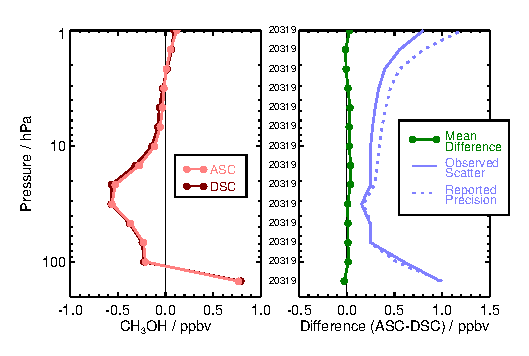
\includegraphics[width=10.0cm]{figures/MLSascdsc_CH3OH_clim}
\caption{(left) Ensemble mean profiles for ascending (light red) and
  descending (dark red) orbit matching pairs of MLS \thisv CH\cs3OH
  profiles averaged over several months of a representative year of
  data (2005).  Symbols indicate MLS retrieval pressure levels.
  (right) Mean differences (ascending$-$descending) in pptv (green
  solid line).  Also shown are the standard deviations about the mean
  differences (light blue solid line) and the root sum square (RSS) of
  the precisions calculated by the retrieval algorithm for the two
  sets of profiles (light blue dashed line). The observed scatter
  about the mean differences and the reported precision values have
  been scaled by 1/$\sqrt{2}$ (to convert from standard deviations of
  differences into standard deviations of individual data points);
  hence the light blue solid line represents the statistical
  repeatability of the MLS measurements, and the light blue dashed
  line represents the expected \mbox{$1\sigma$} precision for a
  single profile.  The thin black lines mark zero in each panel.  The
  number of crossing pairs of measurements being compared at each
  pressure level is noted in the space between the panels.}
\label{fig:mlsascdscCH3OH}
\end{figure}

The precision of the MLS CH\cs3OH data is estimated empirically by
comparing profiles measured at the intersections of ascending (day)
and descending (night) portions of the orbit. Under ideal conditions
(i.e., a quiescent atmosphere), the standard deviation about the mean
differences between such matched profile pairs provides a measure of
the precision of the individual data points. In practice, however,
real changes in the atmosphere may occur over the 12\,h interval
between the intersecting measurement points, in which case the
observed scatter provides an upper limit on the estimate of precision,
assuming that the a priori has a negligible influence on the retrieval
(a reasonable assumption throughout the retrieval range for
CH\cs3OH). The precision estimates were found to be essentially
invariant with time; results for several months of a representative
year of data are shown in Figure~\ref{fig:mlsascdscCH3OH}.  For the
most part, differences between paired profiles are small, implying the
absence of significant systematic ascending / descending biases. The
observed standard deviation is \texttildelow1\,ppbv at 147\,hPa. The
observationally determined precision agrees well with that reported
for each data point by the Level~2 data processing system.  The
estimates reported here represent the precisions at each pressure
level of a single profile; precision can generally be improved by
averaging, with the precision of an average of $N$ profiles being
1/$\sqrt{N}$ times the precision of an individual profile (although
the actual standard error of the mean can in some cases be even
smaller \citep{TooheyAndVonClarmann13}).

\subsection*{Range}

CH\cs3OH is retrieved (and reported in the \texttt{L2GP} files) over the
range 147 to 0.001\,hPa.  However, zonal mean mixing ratios are
negative everywhere at retrieval pressures less than 100\,hPa, as well
as at middle and high latitudes at 100\,hPa.  Thus, with rare
exceptions (such as during extreme events), the v4 \meoh\ data are
considered potentially useful for scientific studies only at 147\,hPa
and at low latitudes at 100\,hPa.

\subsection*{Accuracy}

The impact of various sources of systematic uncertainty has not yet
been quantified for CH\cs3OH as it has for most other MLS products.
This work is planned as part of a dedicated validation exercise for
the \thisv CH\cs3OH data.

\subsection*{Review of comparisons with other datasets}

Detailed comparisons with correlative data sets have not yet been
undertaken.  This work is planned as part of a dedicated validation
exercise for the \thisv CH\cs3OH data.

\subsection*{Data screening}
\label{sec:CH3OHScreening}
\begin{description}
\item[Do not use:] Until more comprehensive validation studies have
  been done, the \thisv CH\cs3OH data should only be used in
  consultation with the MLS science team.
\end{description}

\subsection*{Artifacts}
\begin{itemize}
\item A complete assessment of artifacts in the \thisv CH\cs3OH
  measurements has not yet been performed, but it is known that zonal
  mean mixing ratios are negative everywhere at retrieval pressures
  less than 100\,hPa, as well as at middle and high latitudes at
  100\,hPa.
\end{itemize}

\subsection*{Desired improvements for future data version(s)}
\begin{itemize}
\item Specific improvements in the CH\cs3OH retrieval remain to be
  determined.
\end{itemize}

\begin{table*}[bp]
\caption{Summary of Aura MLS \thisv CH\cs3OH Characteristics}\vspace{0.5ex}
\label{tab:CH3OHSummary}
\begin{minipage}{\linewidth}
\renewcommand{\thefootnote}{\thempfootnote}
\centering\begin{tabular}{ccccl}
\toprule
\parbox[m]{18mm}{\bfseries\centering{Pressure\\ / hPa}} &
\parbox[m]{24mm}{\bfseries\centering{Resolution\\ V $\times$ H%
\footnote{Vertical and Horizontal resolution in along-track direction.} \\ / km}} &
\parbox[m]{18mm}{\bfseries\centering{Precision%
    \footnote{Precision on individual profiles.} \\/ ppbv}} &
\parbox[m]{20mm}{\bfseries\centering{Accuracy\\ / ppbv}} &
\parbox[m]{40mm}{\bfseries\centering{Known Artifacts\\ or Other Comments}} \\
%
\midrule
%
68\,--\,0.001  & ---                             & ---      & ---  & Unsuitable for scientific use\\
%
100            & 5         $\times$ 350          & $\pm$1   & TBD  &
Consult with MLS Science Team \\
%
147            & 4         $\times$ 150          & $\pm$1   & TBD  &
Consult with MLS Science Team \\
%
1000\,--\,215  & ---                             & ---      & ---  & Not retrieved\\
%
\bottomrule
\end{tabular}
\end{minipage}
\end{table*}

%%% Local Variables: 
%%% mode: latex
%%% TeX-master: "v4-x-report"
%%% End: 
 \speciestitle{Chlorine Monoxide}{ClO}{ClO}{%
\item[Useful range:] 147\,--\,1.0\,hPa
\item[Contact:] Michelle Santee, \email{Michelle.L.Santee@jpl.nasa.gov}}

\subsection*{Introduction}

The quality and reliability of the version~2 (v2.2) Aura MLS ClO
measurements were assessed in detail by \citet{SanteeEtal08clo}.  The
ClO product was significantly improved in \prevv
\citep{EOSMLSV33V34Quality}; in particular, the substantial
(\texttildelow0.1--0.4\,ppbv) negative bias present in the v2.2 ClO
values at retrieval levels below (i.e., pressures larger than) 22\,hPa
was mitigated to a large extent, primarily through retrieval of
CH\cs3Cl, which was a new MLS product in \prevv.  The ClO retrieval is
largely unchanged over much of the profile in \thisv.

As in previous versions, in \thisv the standard ClO product is derived
from radiances measured by the radiometer centered near 640\,GHz.
(ClO is also retrieved using radiances from the \mbox{190-GHz}
radiometer, but those data have poorer precision.)  The MLS \thisv ClO
data are scientifically useful over the range 147 to 1\,hPa.  A
summary of the precision and resolution (vertical and horizontal) of
the \thisv ClO measurements as a function of altitude is given in
Table~\ref{tab:ClOSummary}.  The impact of various sources of
systematic uncertainty on the ClO retrievals was quantified in detail
for v2.2 data \citep{SanteeEtal08clo}; Table~\ref{tab:ClOSummary} also
includes estimates of the potential biases and scaling errors in the
measurements compiled from that analysis under the assumption that
most of the sources of uncertainty affect \thisv retrievals in a
similar manner.  The overall uncertainty for an individual data point
is determined by taking the root sum square (RSS) of the precision,
bias, and scaling error terms (for averages, the single-profile
precision value is divided by the square root of the number of
profiles contributing to the average).  More details on the precision,
resolution, and accuracy of the MLS \thisv ClO measurements are given
below.

\subsection*{Resolution}
\onestandardavk{ClO}{ClO}%

The resolution of the retrieved data can be described using
``averaging kernels'' \citep[e.g.,][]{Rodgers00}; the two-dimensional
nature of the MLS data processing system means that the kernels
describe both vertical and horizontal resolution.  Smoothing, imposed
on the retrieval system in both the vertical and horizontal directions
to enhance retrieval stability and precision, degrades the inherent
resolution of the measurements.  Thus, although ClO measurements are
reported at six pressure levels per decade change in pressure (spacing
of \texttildelow2.7\,km), the vertical resolution of the \thisv ClO
data as determined from the full width at half maximum of the rows of
the averaging kernel matrix shown in Figure~\ref{fig:AvkClO} is
\texttildelow3--4.5\,km throughout the retrieval range (with a mean of
\texttildelow3.5\,km).  As in \prevv, in \thisv the averaging kernels
are sharply peaked at all levels, including 147\,hPa.  Thus, although
some degree of overlap is present, the 147\,hPa surface provides
independent information in \thisv.  Figure~\ref{fig:AvkClO} also shows
horizontal averaging kernels, from which the along-track horizontal
resolution is determined to be \texttildelow250--500\,km over most of
the vertical range.  The cross-track resolution, set by the width of
the field of view of the \mbox{640-GHz} radiometer, is
\texttildelow3\,km.  The along-track separation between adjacent
retrieved profiles is 1.5{\degsym} great circle angle
(\texttildelow165\,km), whereas the longitudinal separation of MLS
measurements, set by the Aura orbit, is 10{\degsym}--20{\degsym} over
low and middle latitudes, with much finer sampling in the polar
regions.

\subsection*{Precision}

\begin{figure}
\centering\includegraphics[width=8.4cm]{figures/ComparePrecision2Panel-clo}
\caption{Precision of the (left) \thisv and (right) \prevv MLS ClO
  measurements for four representative days in different seasons (see
  legend).  Solid lines depict the observed scatter in nighttime-only
  measurements obtained in a narrow equatorial band (see text); dotted
  lines depict the theoretical precision estimated by the retrieval
  algorithm.}
\label{fig:ClOPrecProf}
\end{figure}

The precision of the MLS ClO measurements is estimated empirically by
computing the standard deviation of the descending (i.e., nighttime)
profiles in the 20{\degsym}-wide latitude band centered around the
equator.  For this region and time of day, natural atmospheric
variability should be negligible relative to the measurement noise.
As shown in Figure~\ref{fig:ClOPrecProf}, the observed scatter in the
data is essentially unchanged in \thisv, rising from
\texttildelow0.1\,ppbv over the interval 100 -- 3\,hPa to
\texttildelow0.3\,ppbv at 1\,hPa and 147\,hPa.  The smoothing of the
retrieval is turned off above 1\,hPa, and as a consequence the
precision rises steeply above this level.  The scatter in the data is
essentially invariant with time, as seen by comparing the results for
the different days shown in Figure~\ref{fig:ClOPrecProf}.

The single-profile precision estimates cited here are, to first order,
independent of latitude and season, but of course the scientific
utility of individual MLS profiles (i.e., signal to noise) varies with
ClO abundance.  Outside of the lower stratospheric winter polar
vortices, within which ClO is often strongly enhanced, the
single-profile precision exceeds typical ClO mixing ratios,
necessitating the use of averages for scientific studies.  Precision
can generally be improved by averaging, with the precision of an
average of $N$ profiles being 1/$\sqrt{N}$ times the precision of an
individual profile (although the actual standard error of the mean can
in some cases be even smaller \citep{TooheyAndVonClarmann13}).

The observational determination of the precision is compared in
Figure~\ref{fig:ClOPrecProf} to the theoretical precision values
reported by the Level~2 data processing algorithms.  The predicted
precision exceeds the observed scatter, particularly above 15\,hPa,
indicating that the vertical smoothing (regularization) applied to
stabilize the retrieval and improve the precision has a nonnegligible
influence on the results at these levels.  Because the theoretical
precisions take into account occasional variations in instrument
performance, the best estimate of the precision of an individual data
point is the value quoted for that point in the L2GP files, but it
should be borne in mind that this approach slightly overestimates the
actual measurement noise.

\subsection*{Accuracy}

The effects of various sources of systematic uncertainty (e.g.,
instrumental issues, spectroscopic uncertainty, and approximations in
the retrieval formulation and implementation) on the MLS v2.2 ClO
measurements were quantified through a comprehensive set of retrieval
simulations; see \citet{SanteeEtal08clo} for details of how the
analysis was conducted and the magnitude of the expected biases,
additional scatter, and possible scaling errors each source of
uncertainty may introduce into the data.  In aggregate, systematic
uncertainties were estimated to induce in the v2.2 ClO measurements
biases of \mbox{\texttildelow$\pm$0.1\,ppbv} from 100 to 32\,hPa and
less than $\pm$0.05\,ppbv above 22\,hPa and multiplicative errors of
\mbox{\texttildelow$\pm$5--20\%} throughout the stratosphere.
Uncertainties are expected to be of similar magnitude in \thisv, but a
comprehensive \thisv systematic error analysis will be the subject of
future work.

\begin{figure}
\begin{tabular}{@{}l@{}l@{}}
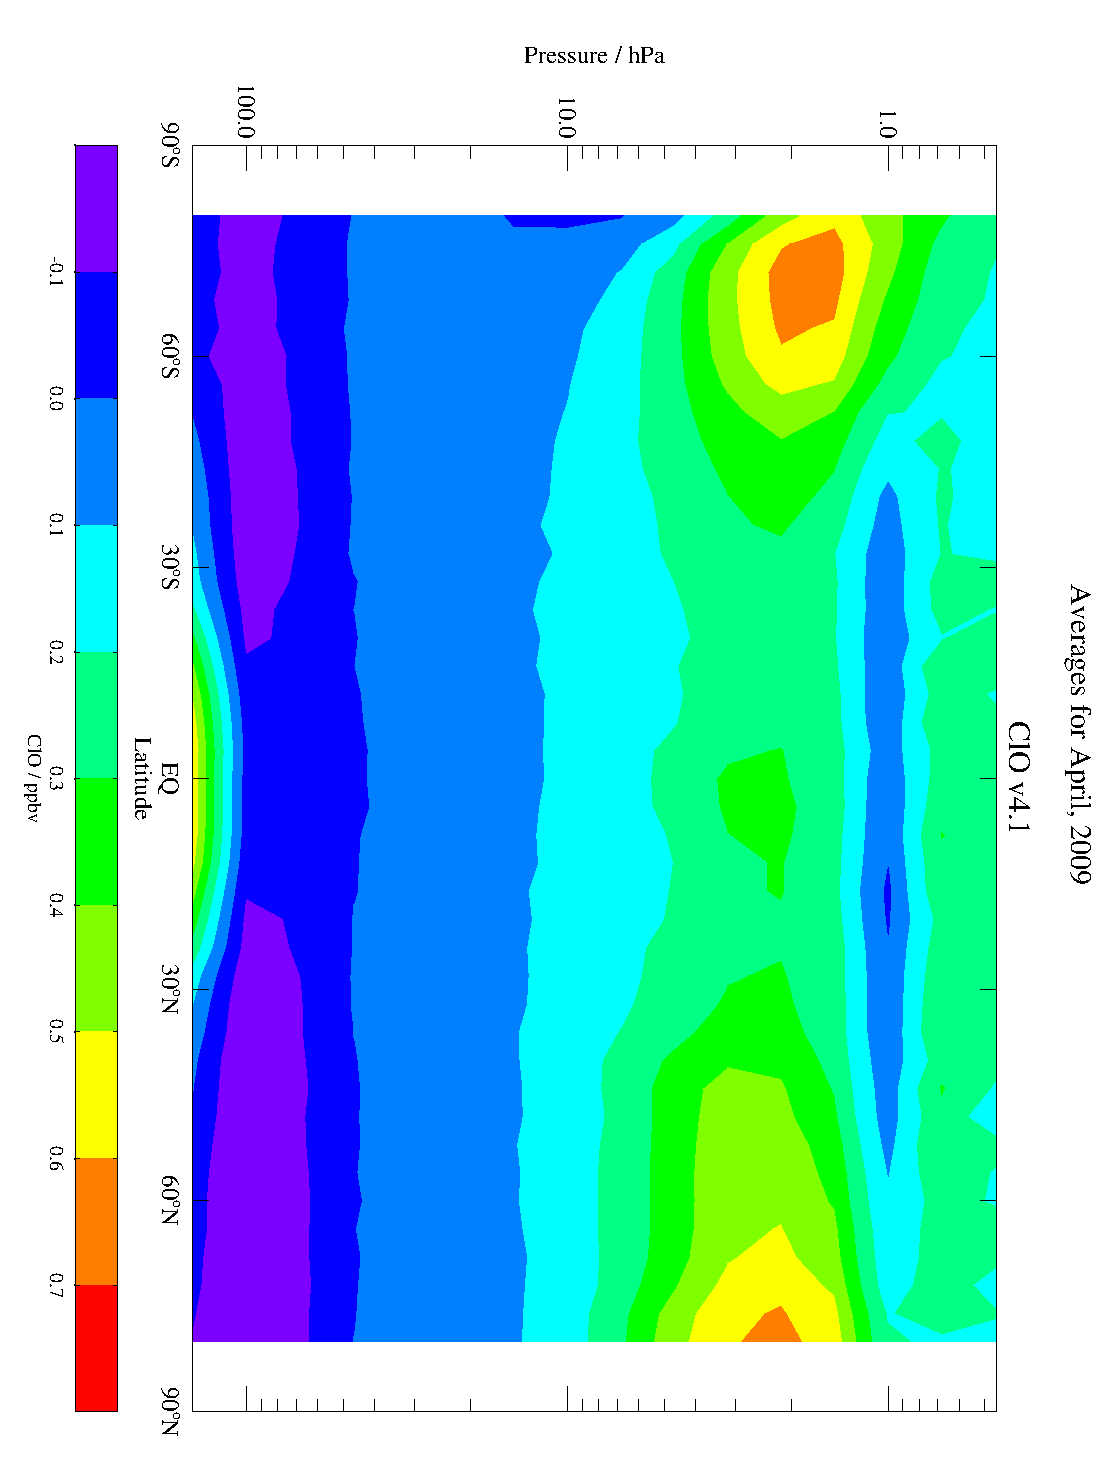
\includegraphics[angle=90,width=0.5\linewidth]{figures/InspectZMContour_ClO--v4-1_ClO--v3-3_2009m04_LatPress-All-noScreen-panel1}&
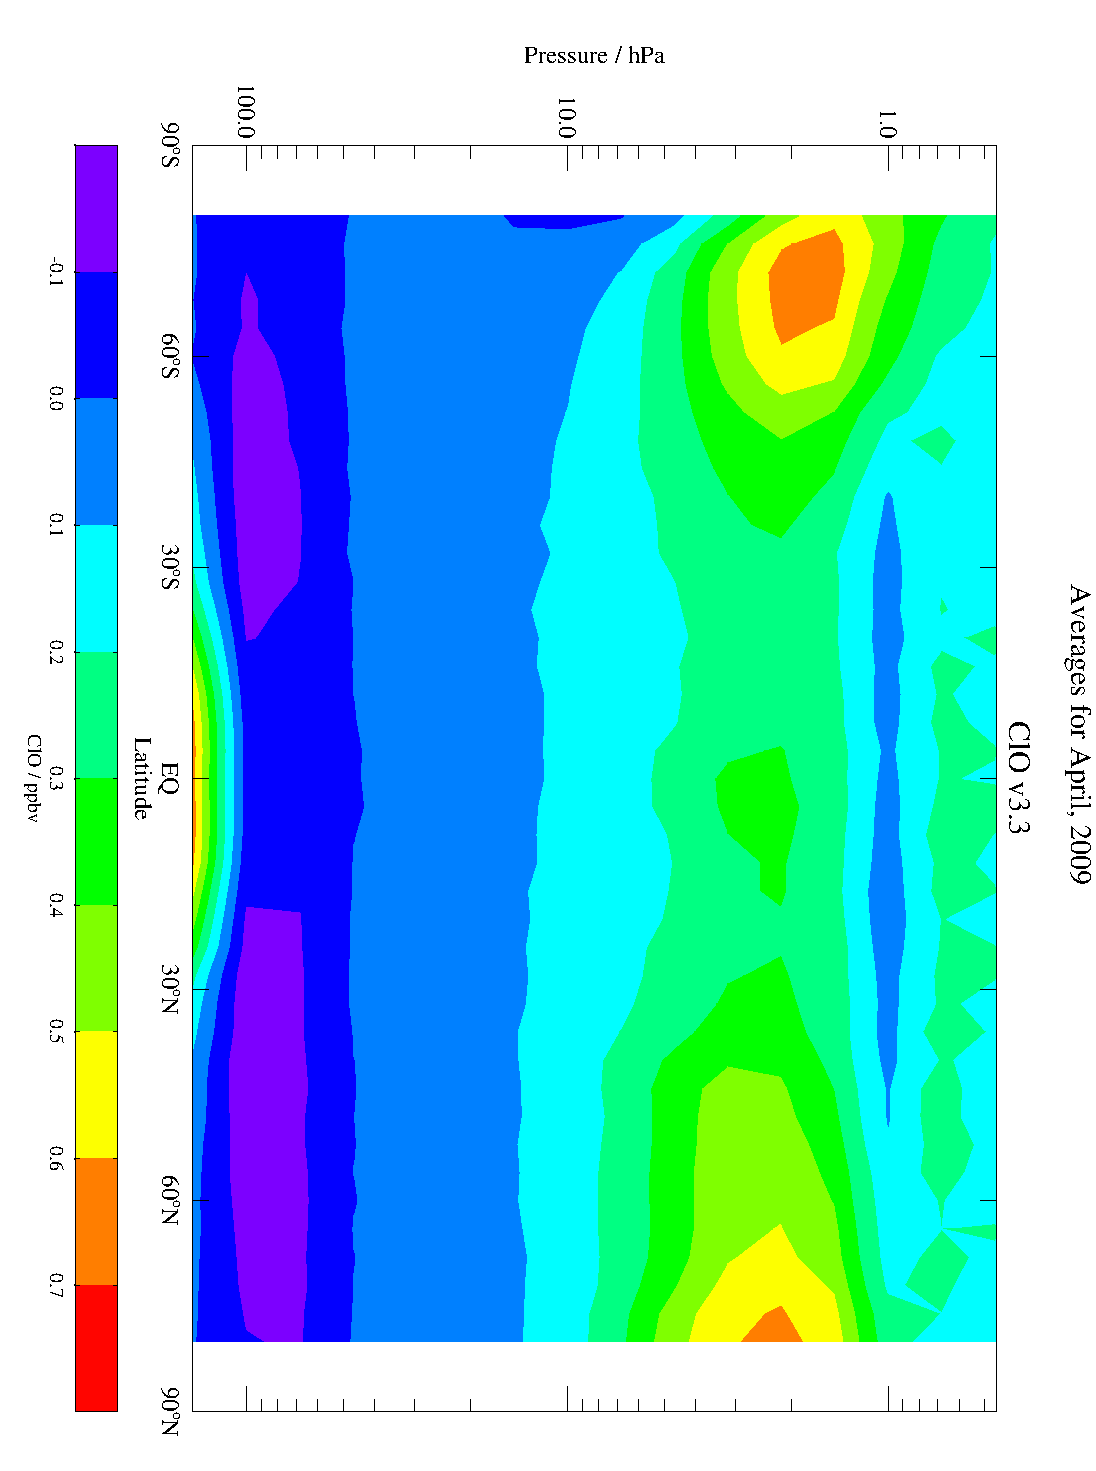
\includegraphics[angle=90,width=0.5\linewidth]{figures/InspectZMContour_ClO--v4-1_ClO--v3-3_2009m04_LatPress-All-noScreen-panel2}\\
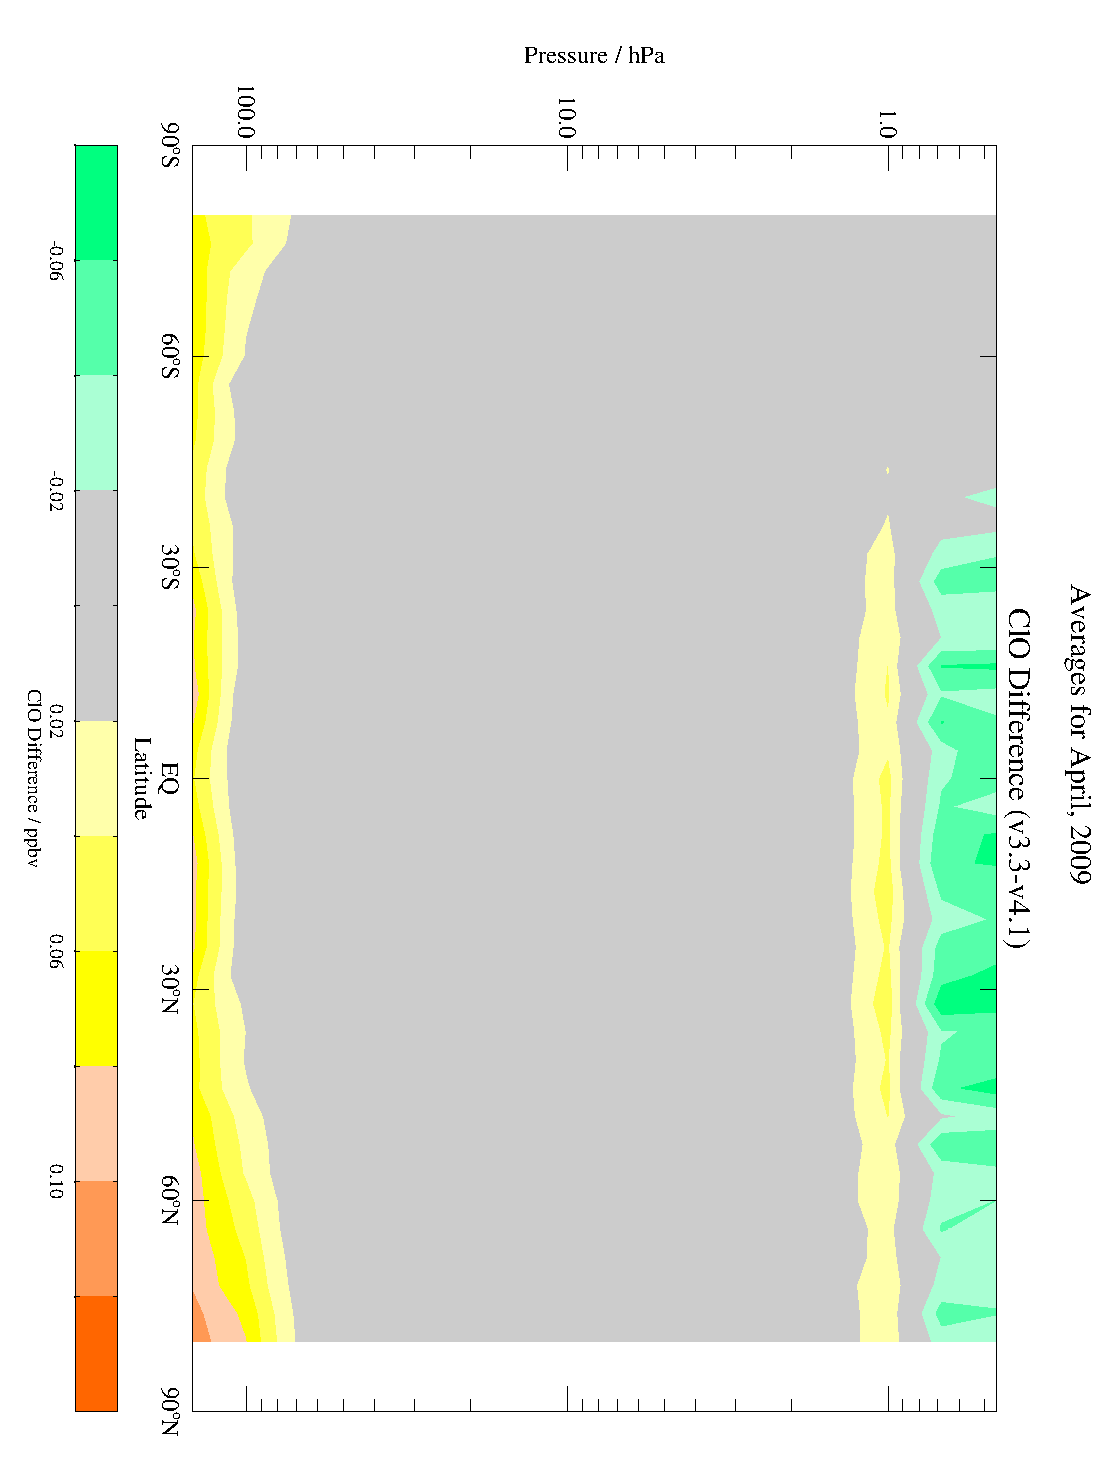
\includegraphics[angle=90,width=0.5\linewidth]{figures/InspectZMContour_ClO--v4-1_ClO--v3-3_2009m04_LatPress-All-noScreen-panel3}&
\raisebox{0.5cm}{\parbox[b]{0.5\textwidth}{%
    \caption{Zonal averages of MLS ClO profiles from the month of April
      2009, showing the MLS \thisv mixing ratios (upper left), the \prevv mixing
      ratios (upper right), and their differences in ppbv (\prevv minus \thisv,
      lower left) as a function of pressure.  The month shown represents
      typical conditions during the Northern Hemisphere late spring /
      Southern Hemisphere early autumn, when ClO is not enhanced in the
      polar lower stratosphere in either
      hemisphere.\label{fig:zmcontourClO}}}}
\end{tabular}
\end{figure}

Differences between \thisv and \prevv ClO mixing ratios are generally
less than 0.04\,ppbv (usually considerably so) at and above (i.e., at
pressures lower than) 68\,hPa, including around the secondary peak in
the ClO profile in the upper stratosphere
(Figure~\ref{fig:zmcontourClO}).  Significant differences (as much as
0.1\,ppbv) are seen at the lowest retrieval levels, however.
Figure~\ref{fig:clov3v2bylat} depicts nighttime mixing ratios for a
single representative day in Southern Hemisphere late spring /
Northern Hemisphere early autumn for which ClO is not enhanced in the
polar lower stratosphere in either hemisphere; a similar plot for a
corresponding day in Northern Hemisphere late spring / Southern
Hemisphere early autumn gives very similar results (not shown). This
figure demonstrates that a small, somewhat latitude-dependent,
negative bias is still evident at 68 and 100\,hPa in \thisv, of
approximately the same magnitude as in \prevv at 68\,hPa but a little
larger at 100\,hPa, especially in the Northern Hemisphere.  At
147\,hPa, \prevv ClO displays a strongly latitudinally varying bias
that is positive at middle and low latitudes and slightly negative in
the polar regions (at least on some days).  In \thisv, ClO mixing
ratios at 147\,hPa are slightly lower than they were in \prevv, and
consequently the low-latitude positive bias has been reduced, although
it remains substantial (exceeding 0.7\,ppbv in some cases), and the
high-latitude negative bias has been exacerbated.

\begin{figure}
\centering\includegraphics[width=10.0cm]{figures/clov4v3bylat-5Nov09}
\caption{Nighttime \thisv (red) and \prevv (black) MLS ClO data as a
  function of latitude for the six lowest retrieval pressure surfaces
  (21--147\,hPa).  The date shown is representative of a typical
  Southern Hemisphere late spring / Northern Hemisphere early autumn
  day for which ClO is not enhanced in the polar lower stratosphere in
  either hemisphere.}
\label{fig:clov3v2bylat}
\end{figure}

In many cases the bias can be essentially eliminated by subtracting
daily gridded or zonal-mean nighttime values from the individual daytime
measurements.  This is not a practical approach under conditions of
continuous daylight in the summer or continuous darkness in the winter
at high latitudes, however.  Moreover, under certain circumstances
inside the winter polar vortices, chlorine activation leads to
nonnegligible ClO abundances even at night.  In this case, taking
day$-$night differences considerably reduces the apparent degree of
chlorine activation.  It is instead recommended that the estimated value
of the bias be subtracted from the individual measurements at each
affected retrieval level.

\begin{figure}
\centering\includegraphics[width=\linewidth,clip=true,trim=0cm 1.5cm 0cm 1.5cm]{figures/plotBiasV4ByMonth}
\caption{Estimates of the bias in MLS \thisv ClO data in 5{\degsym}-wide
  geographic latitude bands on the 147, 100, and 68\,hPa MLS retrieval
  pressure surfaces (see legend).  Each panel shows monthly zonal means
  of \thisv MLS nighttime (solar zenith angle (SZA) $>$ 100{\degsym})
  ClO measurements from 2009 (filled circles).  The grey line marks the
  zero level.  The colored solid lines denote the global mean bias
  estimate at each level for 2009.  The \thisv results are compared
  against corresponding \prevv data (open circles and dotted lines). To
  ensure that ClO was not enhanced, consideration was restricted to
  latitudes equatorward of 50{\degsym}S for the days between 1~May and
  1~November and to latitudes equatorward of 50{\degsym}N for the days
  between 1~December and 1~April.}
\label{fig:cloBiasByMonth}
\end{figure}

To investigate the magnitude of the bias in the \thisv MLS ClO data and
the temporal variations in it, we show in
Figure~\ref{fig:cloBiasByMonth} monthly zonal means of MLS nighttime ClO
measurements from 2009 for pressure levels 147--68\,hPa.  For each
panel, a calendar month of data is binned and averaged in
5{\degsym}-wide latitude bands between $\pm$85{\degsym}.
Figure~\ref{fig:cloBiasByPress} is a similar plot, but encompasses all
of the MLS nighttime ClO data from 2009 for pressure levels
147--10\,hPa.  To guide the eye, the global mean value of the bias from
2009 is indicated for each level (colored solid lines) in both figures.
In Figure~\ref{fig:cloBiasByMonth}, the corresponding \prevv data are
also shown for comparison.  As discussed above, the magnitude, and at
147\,hPa even the sign, of the bias varies with latitude, and
Figures~\ref{fig:cloBiasByMonth} and \ref{fig:cloBiasByPress} make clear
that application of a constant bias correction for all latitudes is not
appropriate.  However, although Figure~\ref{fig:cloBiasByMonth} reveals
significant month-to-month variability, for most studies a
time-invariant latitudinally varying bias correction is adequate.  An
ASCII file containing the altitude- and latitude-dependent \thisv ClO
bias correction values will be made available from the MLS web site once
more data from the mission have been reprocessed to \thisv.

\begin{figure}
  \centering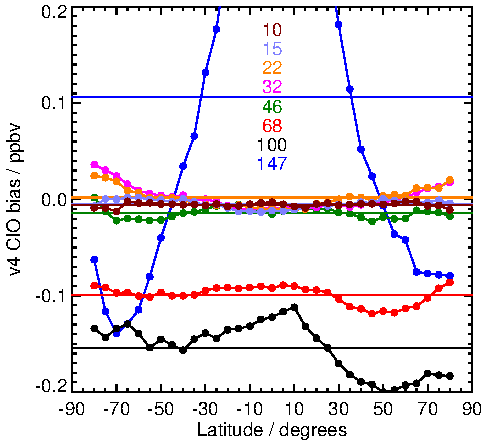
\includegraphics[width=8.4cm]{figures/plotBiasV4}
\caption{Estimates of the bias in MLS \thisv ClO data in
  5{\degsym}-wide geographic latitude bands on MLS retrieval pressure
  surfaces from 147 to 10\,hPa (see legend) calculated for data from
  2009.  To ensure that ClO was not enhanced, consideration was
  restricted to latitudes equatorward of 50{\degsym}S for the days
  between 1~May and 1~November and to latitudes equatorward of
  50{\degsym}N for the days between 1~December and 1~April.  The
  colored solid lines denote the global mean bias estimate at each
  level for 2009.  The large positive bias at low latitudes at
  147\,hPa is cut off in this figure.}
\label{fig:cloBiasByPress}
\end{figure}

\subsection*{Review of comparisons with other  data sets}

Extensive comparisons of MLS v2.2 ClO data with a variety of different
platforms (ground-based, balloon-borne, aircraft, and satellite
instruments) were presented by \citet{SanteeEtal08clo}.  A subset of
those comparisons with \prevv ClO data were reported by
\citet{EOSMLSV33V34Quality}.  Repeating similar analyses for \thisv
data will be the subject of future work.

\subsection*{Data screening}
\label{sec:ClOScreening}
\begin{description}
\item[Pressure range:] \screeningrule{147\,--\,1.0\,hPa}
  \standardrangestatement

  \standardprecisionrule

\item[Status flag:] \screeningrule{Only use profiles for which the
  \texttt{Status} field is zero.}  

  We recommend that all profiles with nonzero values of
  \texttt{Status} be discarded, because of the potential impact of
  cloud artifacts at lower levels.  Note, however, that rejecting in
  their entirety all profiles with nonzero \texttt{Status} may be
  unnecessarily severe at and above (i.e., at pressures equal to or
  smaller than) 46\,hPa, where clouds have negligible impact; thus
  otherwise good-quality profiles with nonzero but even
  \texttt{Status} values may be used without restriction at those
  levels as long as they are removed at larger pressures.  See
  Section~\ref{sec:StatusQuality} for more information on the
  interpretation of the \texttt{Status} field.

\item[Quality:] \qualityrule{1.3} 

  This threshold for \texttt{Quality} (unchanged from \prevv)
  typically excludes less than 1\% of ClO profiles on a daily basis;
  note that it potentially discards some ``good'' data points while
  not necessarily identifying all ``bad'' ones.

\item[Convergence:] \convergencerule{1.05} 

  On a typical day this threshold for \texttt{Convergence} (unchanged
  from \prevv) discards very few (0.3\% or less) of the ClO profiles,
  many (but not all) of which are filtered out by the other quality
  control measures.
\end{description}

\subsection*{Artifacts}
\begin{itemize}
\item Significant biases are present in both daytime and nighttime
  \thisv ClO mixing ratios at and below (i.e., pressures larger than)
  68\,hPa.  The bias should be corrected by subtracting from the
  individual measurements at each affected retrieval level the
  altitude- and latitude-dependent bias estimates given in an ASCII
  file to be made available from the MLS web site once more data from
  the mission have been reprocessed to \thisv.
\end{itemize}

\subsection*{Desired improvements for future data version(s)}
\begin{itemize}
\item Reduce the biases present at the lowest retrieval levels
  (147--68\,hPa).
\end{itemize}

\begin{DIFnomarkup}
\begin{table*}[bp]
\caption{Summary of Aura MLS \thisv ClO Characteristics}\vspace{0.5ex}
\label{tab:ClOSummary}
\begin{minipage}{\linewidth}\small
\renewcommand{\thefootnote}{\thempfootnote}
\centering\begin{tabular}{cccccl}
\toprule
\parbox[m]{18mm}{\bfseries\centering{Pressure\\ / hPa}} &
\parbox[m]{24mm}{\bfseries\centering{Resolution\\ V $\times$ H%
\footnote{Vertical and Horizontal resolution in along-track direction.} \\ / km}} &
\parbox[m]{17mm}{\bfseries\centering{Precision%
\footnote{Precision on individual profiles, determined from observed
 scatter in nighttime (descending) data in a region of minimal atmospheric
 variability.} \\/ ppbv}} &
\parbox[m]{19mm}{\bfseries\centering{Bias\\uncertainty%
    \footnote{Values should be interpreted as \mbox{$2\sigma$}
      estimates of the probable magnitude and, at the higher
      pressures, are the uncertainties after subtraction of the known
      bias.}\gdef\fnTwoSigma{\value{mpfootnote}}\\ / ppbv}} &
\parbox[m]{19mm}{\bfseries\centering{Scaling\\uncertainty\footnotemark[\fnTwoSigma]\\/ \%}} &
\parbox[m]{40mm}{\bfseries\centering{Known Artifacts\\ or Other Comments}} \\
%
\midrule
%
0.68--0.001 & ---   & ---  & ---  & --- & Unsuitable for scientific use\\
%
1.0         & 3        $\times$ 500      & $\pm$0.3 & $\pm$0.05 & $\pm$15\% & \\
%
15--1.5     & 3.5--4   $\times$ 250--400 & $\pm$0.1 & $\pm$0.05 & $\pm$5--15\% & \\
%
46--22      & 3        $\times$ 300--400 & $\pm$0.1 & $\pm$0.1  & $\pm$20\% & \\
%
68          & 3        $\times$ 450      & $\pm$0.1 & $\pm$0.1  & $\pm$20\% &
Latitude-dependent bias\footnote{Correct for the bias by subtracting
  from the individual measurements at this level the
  latitude-dependent bias estimates given in the ASCII file
  to be made available from the MLS web
  site once more data from the mission have been reprocessed to \thisv.}\gdef\fnDirect{\value{mpfootnote}} \\
%
100         & 3        $\times$ 500      & $\pm$0.1 & $\pm$0.1  & $\pm$20\% &
Latitude-dependent bias\footnotemark[\fnDirect] \\
%
147         & 4.5      $\times$ 600      & $\pm$0.3 & $\pm$0.2  & $\pm$40\% &
Latitude-dependent bias\footnotemark[\fnDirect] \\
%
1000--215   & ---   & ---   & --- & --- & Not retrieved\\
%
\bottomrule
\end{tabular}
\end{minipage}
\end{table*}
\end{DIFnomarkup}

%%% Local Variables: 
%%% mode: latex
%%% TeX-master: "v4-x-report"
%%% End: 

 \speciestitle{Carbon monoxide}{CO}{CO}{
\item[Useful range:] 215\,--\,0.0046\,hPa
\item[Contact:] Hugh C. Pumphrey (stratosphere/mesosphere),
   \email{H.C.Pumphrey@ed.ac.uk} \\
  Michael Schwartz (troposphere), \email{Michael.J.Schwartz@jpl.nasa.gov}}

\subsection*{Introduction}
 
Carbon monoxide is retrieved from radiance measurements of two bands in
the MLS 240\,GHz radiometer. Full details are given in
\citet{PumphreyEtal07} and \citet{LiveseyEtal08}.

\subsection*{Differences between \thisv and v03.x}
In the upper troposphere (UT), the primary difference between \thisv CO
and \prevvSlash CO is the reduction in the frequency and severity of
artifacts caused by deep convective clouds.  This was accomplished
through a modification to the manner in which cloud signals are modeled
in the retrievals.  Screening of data has been simplified, fewer
profiles are marked ``bad'' and fewer profiles that appear to contain
cloud artifacts pass through the recommended screening.

A comparison of the two versions in the UTLS for February 2009, shown in
Figure~\ref{fig:BlackSatCO}, includes non-spurious high values from the
plume of the ``Black Saturday'' fire, that are seen in both versions (so
near the black 1:1 line).  Scattering from large particles in convective
cores produces mostly high outliers in v03.30 CO at 215\,hPa, 147\,hPa
and 100\,hPa and low outliers at 68\,hPa and 46\,hPa that are greatly
reduced in \thisv, resulting in the clouds of points away from the 1:1
line.  The ``Black Saturday'' plume produces UTLS CO values outside of
the typically encountered, allowing comparison of non-spurious high
values from the two version, unobscured by the v03.30 cloud-induced
scatter present at lower \thisv mixing ratios.  At the highest values of
the ``Black Saturday'' tails at 100\,hPa and 68\,hPa, values from \thisv
are lower than those from \prevv by $\sim$10\%, but fractional
differences between the versions are smaller at lower mixing ratios. The
screening recommended for \prevv results in a significant amount of
missing data in the tropics, and when the recommended IWC-based
component of \prevv screening is included, a significant fraction of the
``Black Saturday'' non-spurious high values are screened out.

\begin{figure}
  \centering\includegraphics[width=0.9\textwidth]{figures/BlackSatScat_v3v4_noscreen.png}%
  \caption{Version v03.30 CO scattered against v04.20 CO for data from
    February 2009, when the ``Black Saturday'' fire provided a plume of
    non-spurious high-CO outliers, unprecedented in the MLS record.
    This data is unscreened. The 316-hPa retrieval level is shown, but
    is not recommended for scientific use. }
\label{fig:BlackSatCO}
\end{figure}
%
\subsection*{Resolution}
\onestandardavk{CO}{CO}%

Figure~\ref{fig:AvkCO} shows the horizontal and vertical averaging
kernels for \thisv MLS CO\@. Vertical and horizontal resolution are
essentially unchanged from \prevv. The vertical resolution is in the
range 3.5\,--\,5\,km from the upper troposphere to the lower mesosphere,
degrading to 6\,--\,7\,km in the upper mesosphere. Down to the 215\,hPa
level, the vertical averaging kernels are sharply peaked at the level
being retrieved, but while the \mbox{316-hPa} measurement contains contribution
from 316\,hPa, it has a larger contribution from 215\,hPa and a negative
contribution around 100\,hPa of similar magnitude to that at 316\,hPa.
The retrieved value at 316\,hPa is thus more an extrapolation of the
profile higher in the UTLS than it is an independent measurement at
316\,hPa, and it is not recommended for scientific use.  The horizontal
resolution is about 200\,km in the mesosphere, degrading slowly to
300\,km with decreasing height in the stratosphere and more rapidly to
about 460\,km at 100\,hPa and 690\,km at 215\,hPa.

\subsection*{Precision}

The MLS data are supplied with an estimated precision (the field
\texttt{L2gpPrecision}) which is the \emph{a posteriori} precision as
returned by the optimal estimation. The precision of the \thisv CO is
very similar to that of \prevvSlash and is usually smaller (better) than
that of v2.2.  In all versions, the precision is greater than the
scatter observed in the data in regions of low natural variability.
Where the estimated precision is greater than 50\% of the a priori
precision the data will be influenced by the a priori to an undesirably
large extent.  In such cases, \texttt{L2gpPrecision} is set to be
negative (or zero in some cases) to indicate that the data should not be
used.  Figure~\ref{fig:COPrecision} shows both the scatter and estimated
precision for CO, with typical profiles for comparison.
%
\begin{figure}
  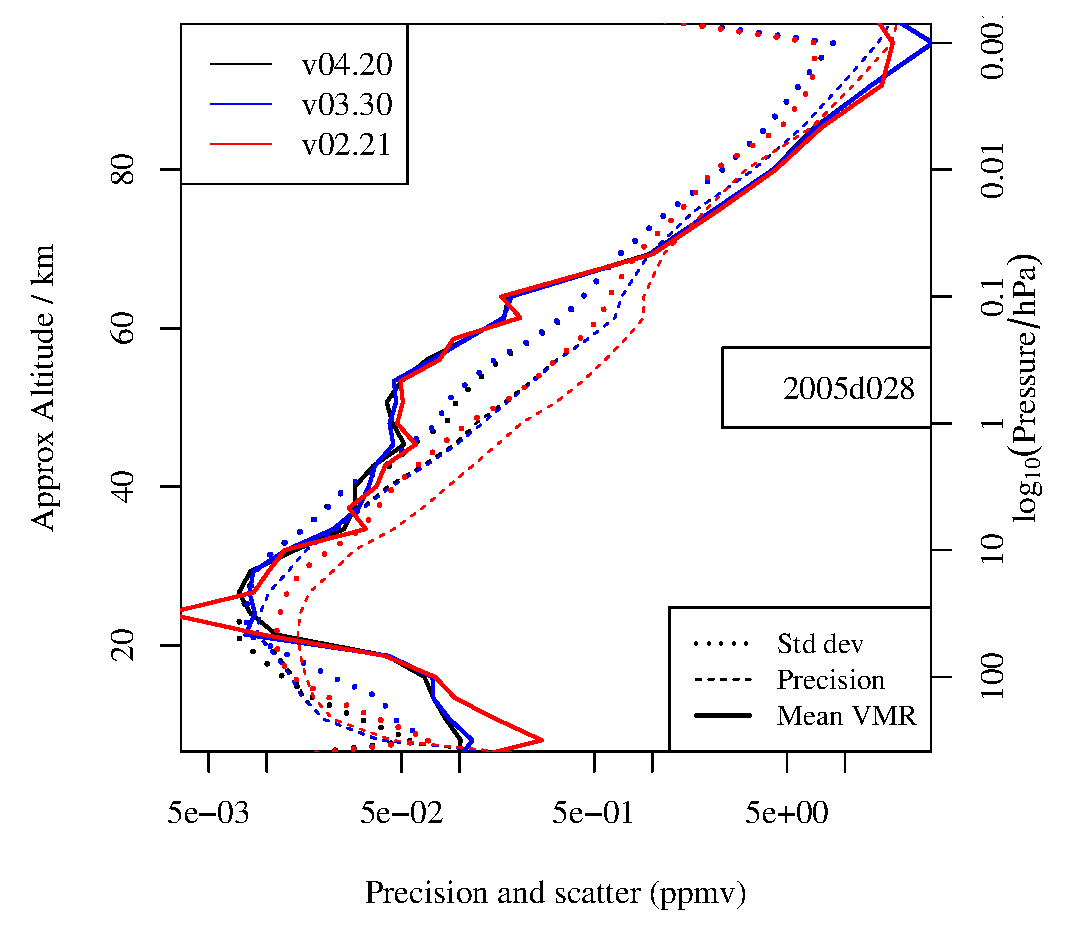
\includegraphics[width=0.495\textwidth]{figures/co-prec-fig-2005d028}\hfill%
  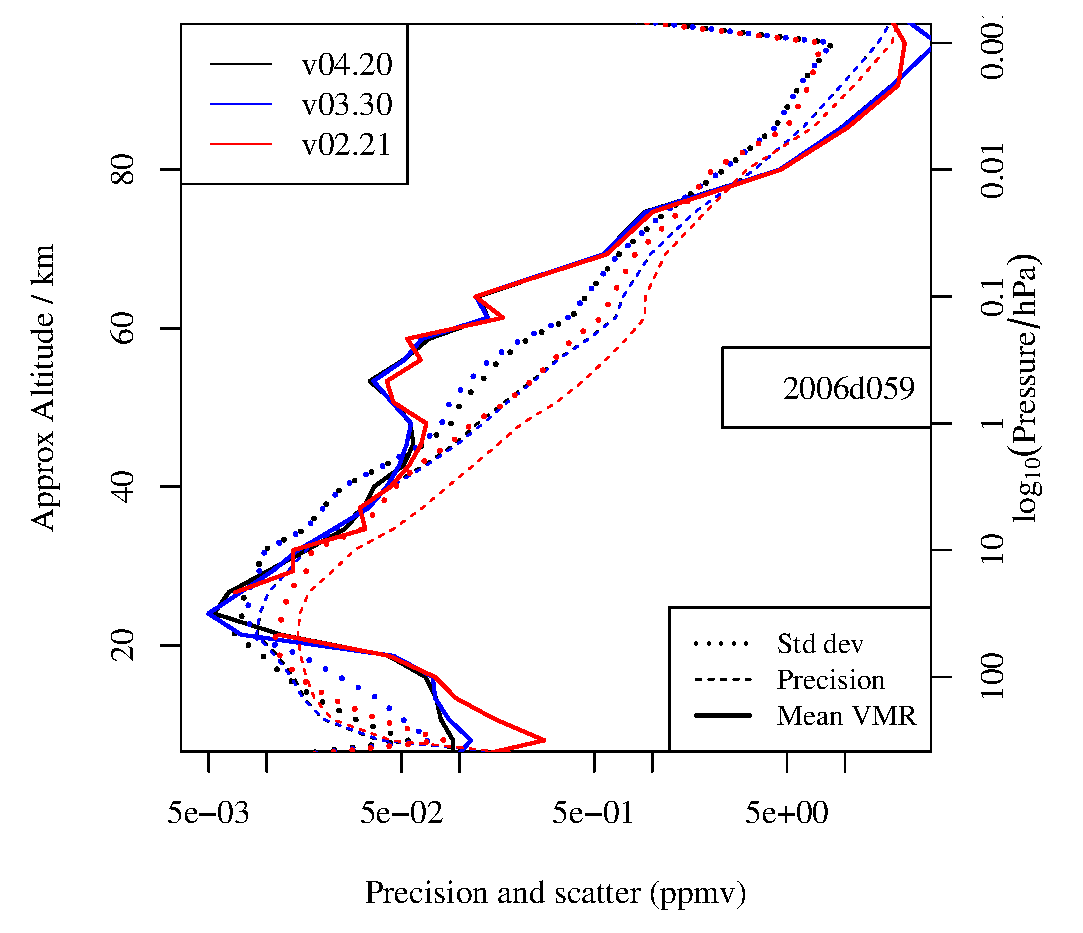
\includegraphics[width=0.495\textwidth]{figures/co-prec-fig-2006d059}
  \caption{Scatter (standard deviation) and (estimated) precision for
    MLS \thisv (black), /prevvShalsh (blue) and v2.2 (red) CO.  The
    statistics shown are generated from all profiles within 20\degsym\
    of the equator on 28 January 2005 and 28 February 2006. Profiles of the
    mean volume mixing ratio (VMR) are shown for comparison. The
    vertical co-ordinate is $16(3-\log_{10}(\mathrm{Pressure / hPa}))$
    so that 16\,km on the axis is exactly 100\,hPa. }
\label{fig:COPrecision}
\end{figure}
%
Note that the random errors are larger than 100\% of the mixing ratio
for much of the vertical range, meaning that significant averaging
(e.g., daily zonal mean or weekly map) is needed to make use of the
data.

\subsection*{Accuracy}

The estimated accuracy is summarized in Table~\ref{tab:COSummary}. In
the middle atmosphere the accuracies are estimated by comparisons with
the ACE-FTS instrument; see \citet{PumphreyEtal07} for further details.
The MLS v2.2 CO data at 215\,hPa showed high (factor of \texttildelow2)
biases compared to other observations.  The morphology, however, was
generally realistic \citep{LiveseyEtal08}.  In \thisv (as in
\prevvSlash) this bias has been essentially eliminated through a change
in the approach to modeling the background radiance upon which the CO
spectral line sits, and a small reduction in the number of MLS spectral
channels considered in the retrieval.

\subsection*{Data screening}
\label{sec:COScreening}
\begin{description}
\item[Pressure range:] \screeningrule{215\,--\,0.0046\,hPa.}
  \standardrangestatement

\standardprecisionrule

\evenstatusrule

\item[Clouds:] Clouds have no impact for pressures of 31\,hPa or
  less. \thisv is much less susceptible to cloud-induced artifacts than
  was v03.x, so screening of the CO product is considerably simplified,
  needing only application of the standard \texttt{Quality} and
  \texttt{Convergence} rules as described below.
 
\item[Quality:] \screeningrule{Only use profiles with \texttt{Quality}
    greater than 1.5.}  Profiles with \texttt{Quality} less than or
  equal to 1.5 comprise 0.7\% of all data, and $\sim$2\% of profiles in
  the tropics.  At 215 hPa in the tropics, the rejected profiles have
  mixing ratios that are, on average, 7\% higher than other tropical
  values and the occurrence rates of high outliers with mixing ratios
  greater than 150\,ppbv is about twice that of the rest of the tropical
  ensemble.  At 100\,hPa there is no significant difference in the means 
  of tropical profiles with Quality less than or greater than 1.5. 

\item[Convergence:] \convergencerule{1.03} This \texttt{Convergence}
  criterion rejects fewer than 0.1\% of profiles.  Almost all of the
  retrievals in the phase that produces \thisv CO converge to their
  target, so \texttt{Convergence} is of limited use in screening.
\end{description}

\subsection*{Artifacts}
\begin{itemize}
\item Positive systematic error of 20\,--\,50\% throughout the mesosphere.
\item Negative systematic error of 50\,--\,70\% near 30\,hPa.
\item Retrieved profiles are rather jagged, especially between 1\,hPa
  (48\,km) and 0.1\,hPa (64\,km). The greater smoothing applied in
  \thisv (and \prevvSlash) compared to v2.2 has reduced this problem
  considerably but has not eliminated it entirely.
\item There is a tendency for negative values to occur at the level
  below a large positive value. The most striking examples occur in the
  polar vortex, where air with high CO mixing ratios descends to the
  mid-stratosphere.  This problem is slightly worse in \thisv and
  \prevvSlash than in v2.2 -- this was considered an acceptable
  trade-off for the less jagged profiles obtained over most of the
  middle atmosphere.
\item Upper-tropospheric \thisv CO retrieved values still show some
  anomalous sensitivity to thick clouds associated with deep convection.
  The screening procedure based upon \texttt{Quality} and
  \texttt{Convergence} that is described above is generally effective in
  removing these artifacts
\end{itemize}

\subsection*{Review of comparisons with other datasets}

In the upper troposphere, comparisons with various in situ CO
observations (NASA DC-8, WB-57 and the MOZAIC dataset) indicate that the
\emph{earlier} MLS v2.2 215\,hPa CO product was biased high by a factor
of \texttildelow2. As in \prevv, this is largely eliminated in \thisv.
Further validation of the \thisv CO in the UT/LS is underway at the time
of this writing.

In the mesosphere, comparisons of the earlier v2.2 MLS CO with ODIN-SMR
and ACE-FTS suggest a positive bias: 30\%\,--\,50\% against ACE-FTS,
50\%\,--\,100\% against SMR. Near 31\,hPa, the MLS values are lower than
SMR and ACE-FTS by at least 70\%. The MLS values have not changed much
between v2.2 and \thisv in the middle atmosphere, so these comparisons
may mostly be considered valid for \thisv.  What change there was
between v2.2 and later versions consists of a slight lowering of the MLS
values, bringing them slightly towards the ACE-FTS data; 20\% is now a
better estimate of the MLS-ACE bias in much of the middle atmosphere
(compared to 30\% with v2.2). The difference between \prevvSlash and
\thisv in the mesosphere is small.

\begin{table}
  \caption{Data quality summary for MLS \thisv\ CO.}
  \vspace{\tablecaptionsep}
\label{tab:COSummary}
\begin{minipage}{\linewidth}
  \centering\begin{tabular}{ccccl}
\toprule
\textbf{Pressure} &
\textbf{Resolution / km} & 
\textbf{Precision} / &
\textbf{Systematic} &  
\textbf{Comment} \\
\textbf{/ hPa} &
\textbf{Vert $\times$ Horiz.} &
\textbf{ppbv} &
\textbf{Uncertainty} \\
\midrule
$<0.001$  &    ---        &   ---   &    ---      & Not retrieved\\
0.0022-0.001  & ---       &   ---   &    ---    & Unsuitable
for scientific use \\
0.0046 &   6.2   $\times$ 200 &  11000  &   $+$20\% to $+$50\%     &  \\
0.01   &   5.9   $\times$ 200 &  4000   &   $+$20\% to $+$50\%  &  \\
0.046  &   5.9   $\times$ 200 &  1200   &    $+$20\% to $+$50\%    &  \\
0.14   &   3.8   $\times$ 200 &  700    &    $+$20\% to $+$50\%    &  \\
1      &   4.1   $\times$ 250 &  130    &    $+$20\% to $+$50\%  &  \\
10     &   5.0   $\times$ 440 &  16     &    $\pm 10$\%    &  \\
31     &   4.9   $\times$ 400 &   9     &    $-$70\% to $-$50\%    &  \\
100    &   4.9   $\times$ 450 &  14     & $\pm$20\,ppbv and $\pm$30\% & \\
147    &   5.1   $\times$ 570 &  15     & $\pm$30\,ppbv and $\pm$30\% & \\
215    &   5.4   $\times$ 690 &  19     & $\pm$30\,ppbv and $\pm$30\% \\
316 & --- & --- & --- & Unsuitable for scientific use\\
$>$316 & --- & --- & --- & Not retrieved \\
\bottomrule
\end{tabular}
\end{minipage}
\end{table}


%%% Local Variables:
%%% mode: latex
%%% TeX-master: "v4-x-report"
%%% End:

 \speciestitle{Geopotential Height}{GPH}{GPH}{%
\item[Useful range:] 261\,--\,0.001\,hPa
\item[Contact:] Michael J. Schwartz,
  \email{Michael.J.Schwartz@jpl.nasa.gov}}

\subsection*{Introduction}

Geopotential height (GPH) is retrieved, along with temperature and the
related assignment of tangent pressures to limb views, primarily from
bands near O\cs2 spectral lines at 118-GHz and 234\,GHz.  The \thisv GPH
product is generally similar to both the v03.x product and to the v02.2
product that is described in \citet{SchwartzEtal08}.

The heights of surfaces of constant geopotential are a property of the
Earth's gravitational field and do not depend upon atmospheric
conditions.  Geopotential differences between surfaces are equal to the
integral with height of the gravitational acceleration, $g$.  GPH is
geopotential difference from the Earth's surface geopotential to a given
location, scaled by the mean-sealevel gravitational acceleration, $g_0$,
to give units of height.

MLS products, including GPH and temperature, are reported on pressure
surfaces, but pressure, temperature and height depend upon one another
through assumed hydrostatic balance and the gas law.
\begin{equation}
\frac{1}{g_o} \int g\,dh = \frac{R}{M g_o}\int T\,dP/P,
\end{equation}
where $M$ is the molar mass of air and $R$ is the gas constant.

Thus a retrieval of a temperature profile on fixed pressure surfaces
also determines GPH differences between those surfaces, and so
determines the GPH profile to within an additive constant.  Absolute
pointing cannot be inferred from radiometric information and must be
obtained, for each profile, from the spacecraft orbit/attitude system
and the instrument scan model.  By convention, this additional degree of
freedom is taken to be the height of the 100-hPa reference level, but
this choice is arbitrary, as the reference is an additive offset to the
entire profile.

Table~\ref{tab:GPHSummary} summarizes \thisv measurement precision,
modeled accuracy and observed biases.  The following sections provide
details.

\subsection*{Differences between \thisv and previous versions}
The \thisv GPH product is taken from the \texttt{CorePlusR3} retrieval
phase along with a number of standard products that depend upon
radiances of the 240-GHz radiometer.  The previously released v02.2x and
v03.x GPH products were taken from a preliminary ``Core'' retrieval
phase.  Since these GPH profiles are retrieved simultaneously with the
\texttt{CorePlusR3} products and are assumed in the \texttt{CorePlusR2}
and \texttt{CorePlusR4} retrievals, GPH and the retrieved constituents
should be, in some sense, more internally consistent than they were in
previous versions.

These previous versions of MLS GPH were referenced to the WGS84
ellipsoid, a simple model of the Earth's surface but not a surface of
constant geopotential.  \thisv uses a surface of constant geopotential,
the Earth Gravitational Model 1996 (EGM96) geoid, as its zero GPH
surface.  The magnitude of the static, latitude/longitude-dependent
difference between the geoid and ellipsoid exceeds $\pm$100\,m in
places, as is shown in Figure~\ref{fig:geoidheight}.  This EGM96-WGS84
difference is a bias that should be subtracted from previous versions'
GPH before they are compared to \thisv GPH.  These differences, if not
corrected, will result in an erroneous additive contribution to
geostrophic winds calculated from v03.x and v02.x GPH at all levels.
\begin{figure}
\centering\includegraphics[clip=true,trim=2cm 0cm 0cm 4cm, width=0.7\linewidth]{figures/EGM96-WGS84}
\caption{The height of the EGM96 geoid from the WGS84 ellipsoid.  These
  values should be subtracted from MLS v03.x and earlier GPH values to give
  geopotential heights referenced to the Earth's mean sea level
  geopotential.  \thisv GPH does not include this bias term.}
\label{fig:geoidheight}
\end{figure}

After correction of v03.3x for the EGM96-WGS84 bias, \thisv GPH values
are found to be somewhat higher at high latitudes than are those of the
v03.3x product, with typical 100-hPa mean differences of 50\,m in the
high northern latitudes, 30\,m in high southern latitudes and close to
zero bias in the tropics.  Latitudinally and seasonally dependent
differences between \thisv and ellipsoid-referenced \prevvSlash 100-hPa
GPH are shown in Figure~\ref{fig:v4-v3_100hPaGPH_2005} for the years
2005 and 2009.  These differences are very similar for ascending and
descending parts of the orbits, and the two are averaged in this figure.
The details of these differences vary between years, but the morphology
is similar.
\begin{figure}
\centering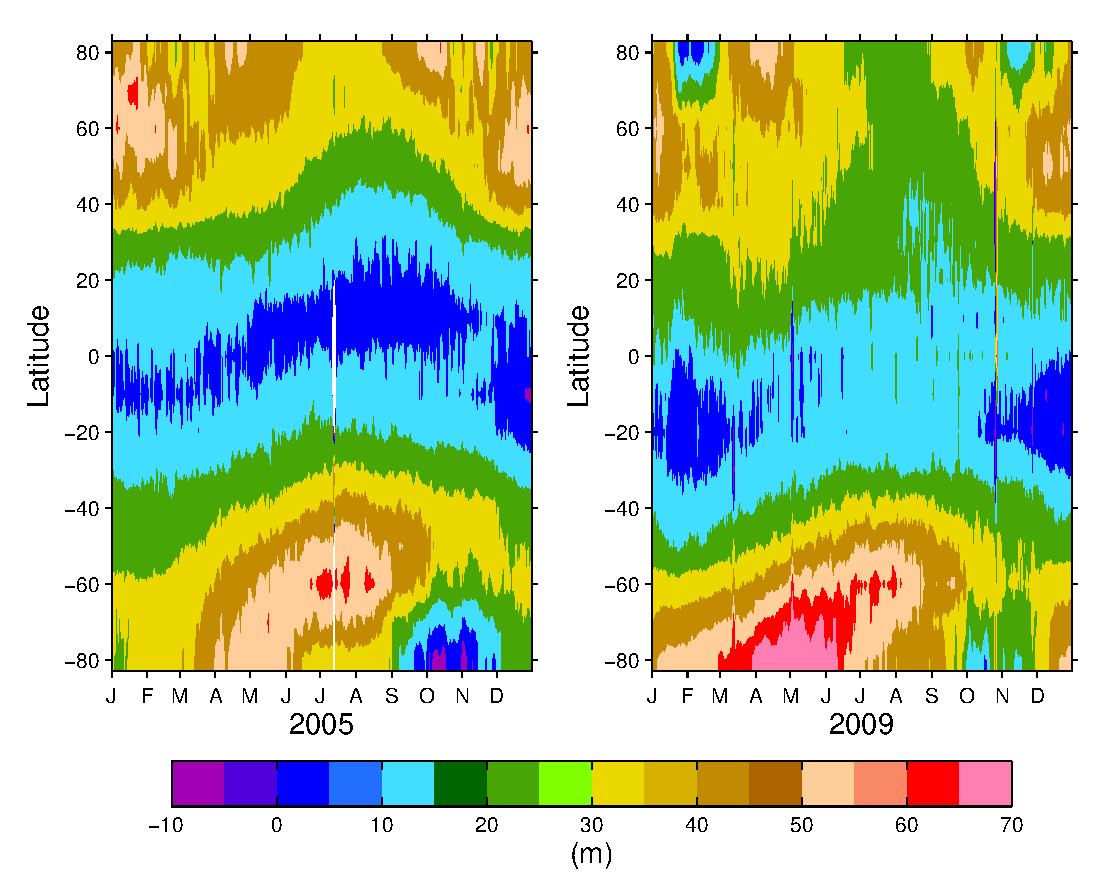
\includegraphics[width=0.7\linewidth]{figures/v4-v3_100hPaGPH_2005-2009_bylat}
\caption{Differences between \thisv and ellipsoid-referenced v03.30 100-hPa GPH for 2005 and
  2009 are shown as functions of latitude and day of year.}
\label{fig:v4-v3_100hPaGPH_2005}
\end{figure}

\subsection*{Comparison to GEOS-5 Analysis}
After removal of the geoid correction from v03.3x GPH, there remains a
latitudinally and seasonally-varying bias between MLS and GEOS-5 that is
also present in \thisv GPH.  Figure~\ref{fig:GPHv3_lat_annual} shows
this pattern in the difference between geoid-corrected v03.3x and GEOS-5
100-hPa GPH.  This pattern is very similar in \thisv.
\begin{figure}
\centering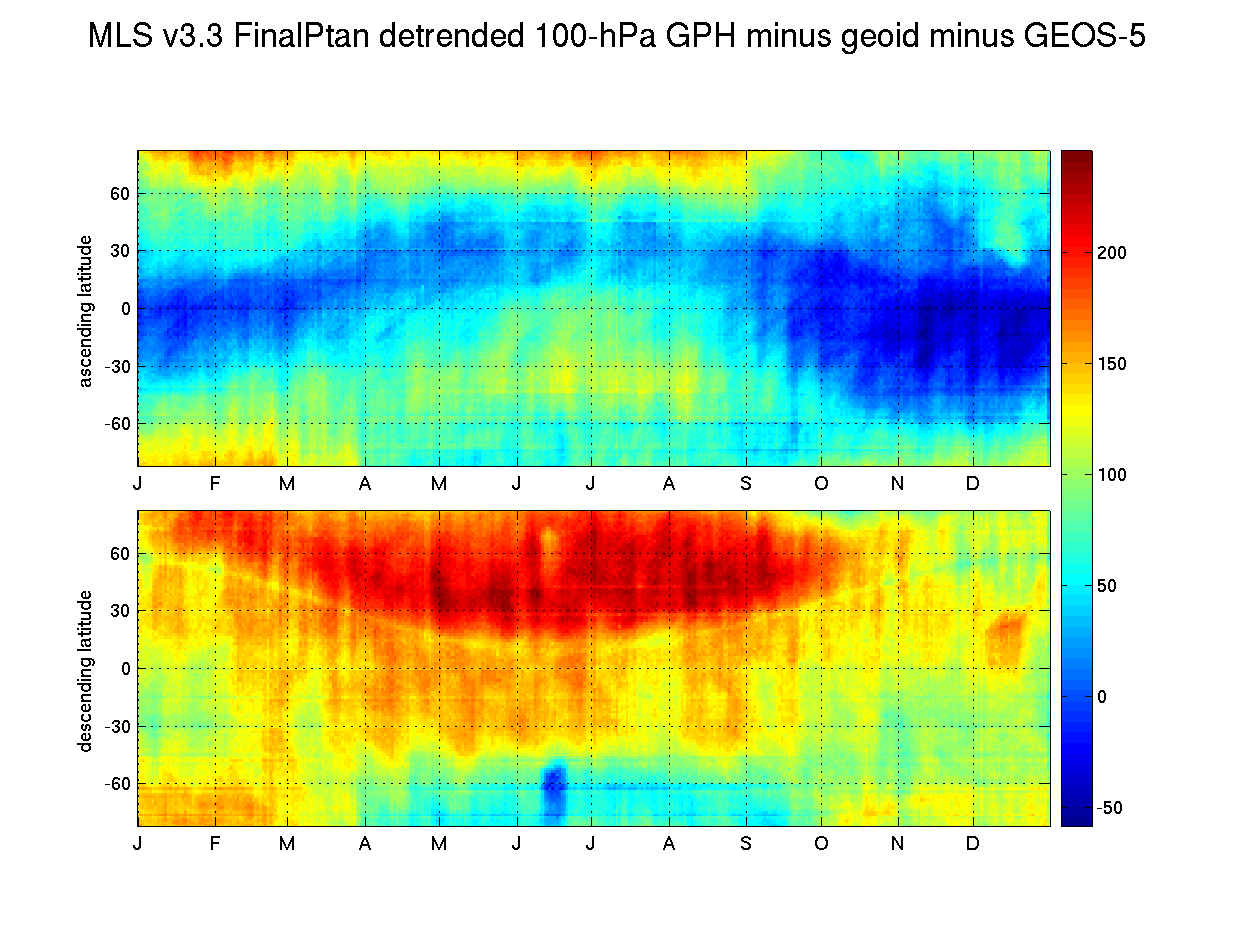
\includegraphics[width=0.7\linewidth,clip=true,trim=1cm 1cm
1cm 2cm]{figures/GPH_geoid_correction2A}
\caption{Annually-repeating biases between MLS 100-hPa GPH and GEOS-5.2
  100-hPa GPH as functions of ascending and descending latitude and of
  day of year.  These biases were computed based upon data from the
  years 2005--2012.}
\label{fig:GPHv3_lat_annual}
\end{figure}

Some of this annually-repeating ``bias'' may result from
annually-repeating geophysical information captured by MLS that is not
in the GEOS-5 analysis.  However, the large ascending-descending
differences are almost certainly not primarily diurnal effects.  The
fidelity with which these patterns annually repeat suggests that they
may result from thermal distortions of the spacecraft/instrument that
vary annually due to the eccentricity of the Earth's orbit, or perhaps
from orbit/attitude errors from the star trackers that provide the
spacecraft-attitude information.  The same star fields are viewed each
year at the same date and orbit position.

\begin{figure}
\centering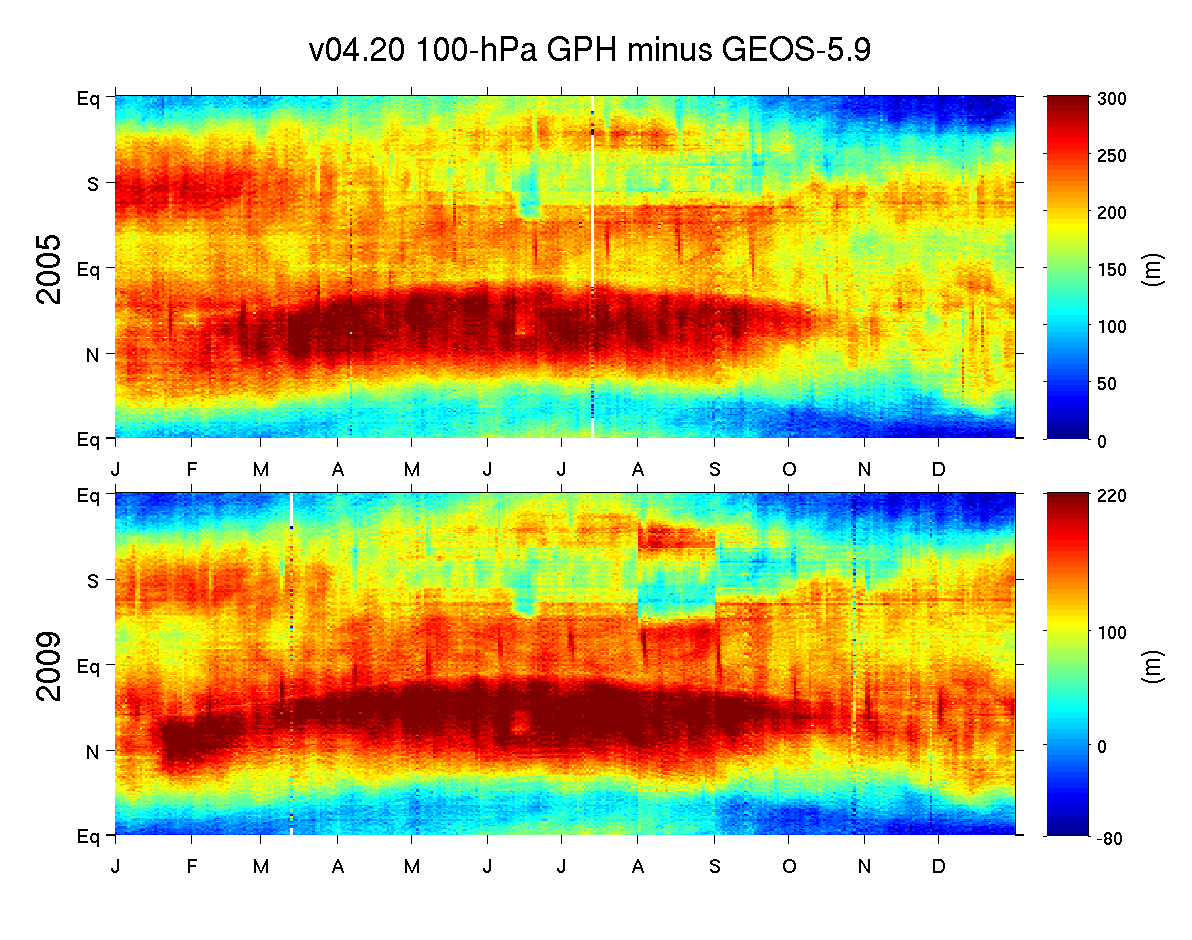
\includegraphics[width=0.7\linewidth]{figures/v4GPH_2005_2009_byOGA}
\caption{Daily-binned differences between \thisv and GEOS-5.9 100-hPa
  GPH as functions of orbital position.  Orbital position, from the bottom of each
  panel, ascends from the equator to the northern terminator, descends
through the equator to the southern terminator and then ascends to the
equator.}
\label{fig:v4GPH_2005_2009_byOGA}
\end{figure}

Figure~\ref{fig:v4GPH_2005_2009_byOGA} shows daily-binned differences
between \thisv and GEOS-5.9 100-hPa GPH as functions of orbital
position. The patterns are extremely similar in the two years and to the
annually repeating \prevv residual shown in
Figure~\ref{fig:GPHv3_lat_annual}, but 2009 is $\sim$80\,m lower than
2005 due to a decreasing trend in MLS \thisv GPH.

As of the drafting of this document, the entire MLS data record has not
been reprocessed with \thisv algorithms, but 11 years of Januarys have
been completed and the monthly-averaged differences between MLS \thisv
100-hPa GPH and GEOS-5.9 100-hPa GPH is shown in
Figure~\ref{fig:GPHv0420_trend_January}.  There is a clear downward
trend of $\sim$100\,m in the first 4 years of the mission, 2005--2008,
with a further $\sim$15\,m decrease in 2009--2014.  This trend is in the
MLS GPH and is not evident in the GEOS-5.9 time series.  Analysis of
\prevv GPH, for which the entire MLS record has been processed, shows
the same global decreasing trend. It is important to emphasize that MLS
radiances do not provide absolute pointing information, but only GPH
differences between pointing.  Absolute pointing comes from spacecraft
ephemeris and attitude data and the instrument scan model.  The origins
of the trend is a topic of current research, but it is likely not
primarily of geophysical origin.

\begin{figure}
  \centering\includegraphics[width=0.7\linewidth]{figures/GPHv0420_trend_January}
\caption{January monthly-binned differences between \thisv and GEOS-5.9 100-hPa
  GPH.}
\label{fig:GPHv0420_trend_January}
\end{figure}

When both the trend and the annually repeating bias are removed from
\prevv, the standard deviation of the residual differences between the
bias-corrected MLS and GEOS-5 100-hPa GPH is on the order of 20\,m, and
a similar result is expected for \thisv.

The last four profiles of each day show increased rates of outliers
relative to GEOS-5 temperature, compared to other profile positions in
the day in version~4.20 (fixed in version~4.22).  These outliers can be
as large as 50\,K at at some levels.  A recommendation to discard the
last 4 profiles of each day for both temperature and GPH (as well as
RHI) has been added to recommended screening for v4.20 (not needed for
v4.22).

\subsection*{Vertical resolution}

The GPH profile is vertically-integrated temperature, so its vertical
resolution is not well-defined.  The vertical resolution of the
underlying temperature given in Section~\ref{sec:StandardTemperature} is
repeated in Table~\ref{tab:GPHSummary}.

\subsection*{Precision}

MLS \thisv GPH precision is summarized in Table~\ref{tab:GPHSummary}.
Precision is the random component of measurements that will average-down
if a measurement is repeated.  The retrieval software returns an
estimate of GPH precision only for the 100\,hPa reference level, as this
is the only element included in the MLS ``state vector.''  GPH precision
at other standard-product profile levels (summarized in column~2 of
Table~\ref{tab:GPHSummary}) is calculated from the GPH precision at the
reference level and the profile of temperature precisions.  Calculated
precision values are \texttildelow35\,m from 261\,hPa to 100\,hPa,
\texttildelow45\,m at 1\,hPa, \texttildelow110\,m at 0.001\,hPa.
Off-diagonal elements of the temperature/GPH error covariance matrix are
neglected in this GPH-precision-profile calculation, but resulting
errors are believed to be small (\texttildelow5\,m near 100\,hPa.)

\subsection*{Accuracy}

The accuracy of the v2.2 GPH was modeled based upon consideration of a
variety of sources of systematic error, as discussed in
\citet{SchwartzEtal08}. \thisv accuracy is believed to be substantially
similar and the results of the v2.2 calculations are given in column
four of Table\,\ref{tab:GPHSummary}. Of the error sources considered,
modeled amplifier non-linearity had the largest impact, just as is the
case with the calculation for temperature.

The second terms in column four are model-based estimates of the bias
magnitude from other sources including uncertainty in
pointing/field-of-view, uncertainty in spectroscopic parameters, and
retrieval numerics.  The combined bias magnitudes due to these sources
is 100\,--\,150\,m.

``Observed bias uncertainty'' in Table~\ref{tab:GPHSummary} is an
estimate of bias based upon comparisons with analyses and with other
previously-validated satellite-based measurements.  These comparisons
were made using MLS v2.2, but as the biases between v2.2 and \thisv GPH
are generally less than 50\,m from 261\,--0.1\,hPa and reasonably
constant, these results hold for \thisv as well.  The primary sources of
correlative data were the Goddard Earth Observing System, Version 5.0.1
data assimilation system (GEOS-5) \citep{ReineckerEtal07}, used in the
troposphere and lower stratosphere, and the Sounding of the Atmosphere
using Broadband Radiometry (SABER) \citep{MlynczakAndRussell95}, used in
the upper stratosphere through the mesosphere.  MLS has a 150\,m high
bias relative to analyses (GEOS-5) at 100-hPa that drops to 100\,m at
1\,hPa.  Biases with respect to SABER are small at 0.1\,hPa but
increasingly negative at higher levels, reaching -600\,m at 0.001\,hPa,
but with significant latitudinal and seasonal variability.

\subsection*{Known Artifacts}
To maintain its position in the ``A-Train'' constellation of satellites,
the Aura spacecraft periodically executes ``inclination adjustment
maneuvers'' (IAMs) involving large changes in spacecraft yaw and firing
of thrusters.  There were 39 such maneuvers in the first 10 years of
operation.  Large systematic errors in spacecraft reported attitude have
been found in the first orbit that follows the return to nominally good
attitude data after these maneuvers, apparently due to the ringing of a
Kalman filter in the attitude measurement system. Since MLS GPH relies
on spacecraft attitude for its absolute reference, these attitude errors
result in large systematic errors in GPH, typically reaching +3500\,m in
the first eighth of the orbit and -30\,m in the second quarter orbit
after the nominal ``end of maneuver''.  The large positive errors almost
always occur on ascending orbits from near Australia, crossing the
Indian Ocean and, at $\sim$3500\,m amplitude, are large enough to
significantly bias even long-term averages.  A file of start and stop
times for data to be avoided is maintained on the MLS website:
\href{http://mls.jpl.nasa.gov/cal/issues.txt}{\texttt{http://mls.jpl.nasa.gov/cal/issues.txt}}.


\subsection*{Data screening}
\label{sec:GPHScreening}

GPH should be screened in much the same way as is temperature:

\begin{description}
\item[Pressure range:] \screeningrule{261\,--\,0.001\,hPa.}
  \standardrangestatement

  \standardprecisionrule GPH precision is set negative at and beyond any
  level in the integration of temperature away from the 100-hPa
  reference level where temperature has negative precision.

\evenstatusrule

\item[Clouds:] Thick clouds are believed have some impact on \thisv GPH
  measurements in the upper troposphere (261\,--\,100\,hPa).
  Tropospheric GPH may be screened using the ice water content (IWC)
  product, rejecting profiles between 261--100\,hPa for which the
  215\,hPa value of IWC is greater than 0.005\,mg/m$^3$.

\item[Quality:] Only use profiles with \texttt{Quality} greater than 0.2
  for the 83\,hPa level and smaller pressures, and profiles with
  \texttt{Quality} greater than 0.9 at larger pressures of 100\,hPa and
  larger.

\item[Convergence:] \convergencerule{1.03} Use of this threshold
  typically discards less than 0.1\% of profiles and is primarily a
  safeguard against profiles with extremely poor convergence.

\item[End of day (v4.20 only):] The last four profiles of each day show
  greatly increased rates of large temperature departure from \emph{a
    priori}.  Accordingly the last four profiles of the GPH product each
  day should not be used.  Note that this issue was fixed in v4.22.

\item[IAMs:] Large errors in reported spacecraft attitude have been
  found following the spacecraft inclination adjustment maneuvers that
  occur $\sim$4 times per year.  A file of times at which GPH should not
  be used is maintained on the MLS website:
  \href{http://mls.jpl.nasa.gov/cal/issues.txt}%
  {\texttt{http://mls.jpl.nasa.gov/cal/issues.txt}}.
\end{description}

\subsection*{Desired improvements for future data version(s)}

Reduction of seasonally and latitudinally-repeating systematic errors in
GPH that may be the result of errors in the absolute pointing
information from the spacecraft attitude and ephemeris data stream is an
area of ongoing research.  Undertanding the decreasing trend in MLS
global mean GPH, particularly in the first four years of the mission is
an area of active research.
  
\begin{table}
\label{tab:GPHSummary}
\begin{minipage}{\linewidth}
\centering\begin{tabular}{ccccl}
\toprule
\textbf{Region} & 
\parbox[m]{22mm}{\centering\textbf{Resolution\\ \mbox{Vert. $\times$ Horiz.} / km}} &
\parbox[m]{18mm}{\centering\textbf{Precision\footnote{Precision on individual profiles} \\/ meters}} &
\parbox[m]{20mm}{\centering\textbf{Observed bias\\uncertainty\\ / m}} &
\textbf{Comments} \\
\midrule
$<$0.001\,hPa & --- & --- & --- & Unsuitable for scientific use \\
0.001\,hPa          & 10--13 $\times$ 220  & $\pm$110 & $-$450 & \\
0.01\,hPa           & 8--12 $\times$ 185  & $\pm$85   & $-$100 & \\
0.1\,hPa            & 6 $\times$ 165   & $\pm$60   &  0  & \\
1\,hPa              & 7 $\times$ 165   & $\pm$45   & 100 & \\
10\,hPa             & 4.3 $\times$ 165 & $\pm$35   & 100 & \\
100\,hPa            & 5.2 $\times$ 165 & $\pm$30   & 150 & \\
261\,hPa            & 5.3 $\times$ 170 & $\pm$35   & 150 & \\
1000\,--\,316\,hPa & ---      & ---             & ---     & Unsuitable for scientific use\\
\bottomrule
\end{tabular}
\end{minipage}
\end{table}

%%% Local Variables: 
%%% mode: latex
%%% TeX-master: "v4-x-report"
%%% End: 
 \speciestitle{Water Vapor}{H\cs2O}{H2O}{
\item[Useful range:] 316\,--\,0.002\,hPa
\item[Contact:] Alyn Lambert (stratosphere/mesosphere),
  \email{alyn.lambert@jpl.nasa.gov} \\
  William Read (troposphere), \email{william.g.read@jpl.nasa.gov}}

\subsection*{Introduction}

The standard water vapor product is taken from the 190-GHz
``\texttt{CorePlusR2}'' retrieval. The vertical grid for H\cs2O is: 12
levels per decade change in pressure (LPD) for 1000\,--\,1 hPa, 6\,LPD
for 1.0\,--\,0.1\,hPa, and 3\,LPD for 0.1\,--\,10\cp{$-$5}\,hPa. The
horizontal grid is every 1.5\degsym along the orbit track.  H\cs2O is
unusual among MLS products in that it is assumed that the logarithm of
the mixing ratio, and not mixing ratio itself, varies linearly with log
pressure; although, H\cs2O, like the other MLS constituents is retrieved
in VMR (not $\log$ VMR). Vertical and horizontal interpolations of
H\cs2O should be performed in $\log(\text{VMR})$ space.

The MLS \thisv H\cs2O between 1000 and 383\,hPa is taken from a
retrieval of relative humidity with respect to ice (RHi) product,
converted to specific humidity using the Goff-Gratch vapor pressure over
ice equation.  This RHi retrieval is not vertically resolved, and all
levels between 1000 and 383\,hPa are assumed to have the same RHi.  See
Section~\ref{sec:StandardRHI} for more information. Validation of MLS
v2.2 water vapor is presented in \citet{ReadEtal07} and
\citet{LambertEtal07}.  This section reiterates the key information from
those studies, and updates them for \thisv.  Table~\ref{tab:H2OSummary}
gives a summary of MLS \thisv H\cs2O precision, resolution, and accuracy.

\subsection*{Changes from \prevv}

The main H\cs2O differences between \thisv and \prevvSlash relate to
cloud screening and improvements in the ``\texttt{InitUTH}'' initial
upper tropospheric and lower stratospheric humidity estimation phase
that produces the first guess and sets smoothing constraints on the
H\cs2O profile retrieved in the final retrieval phase that produces the
standard product. There have been no spectroscopy changes either in
linewidth or continuum charaterization between \thisv and
\prevvSlash. An improved cloud detection methodology has been developed
for \thisv that does a better job of rejecting cloudy radiances that are
likely to cause poor fits and corrupted profiles. The number of
erroneous spikes in the upper troposphere has been reduced in \thisv
relative to \prevv. The \texttt{InitUTH} phase retrieves H\cs2O on a
more coarse 6-LPD grid. The InitUTH H\cs2O is used for the initial guess
for the final 12-LPD retrieval and sets smoothing constraints for the
profile shape instead of smoothing to the shape of a climatological
\emph{a priori} profile.  The \texttt{InitUTH} phase has been expanded
to use more channels and better forward model representations to improve
its retrieval accuracy. In addition, the retrieval range has been
expanded to have its top moved from 100\,hPa (in \prevv) to 10\,hPa (in
\thisv), for a more seamless transition from the troposphere to the
stratosphere. Simulation studies show that these changes have improved
the agreement between the ``truth'' profiles used to produce the
simulated radiances and the retrieved profiles in the 316\,--\,215-hPa
levels.

\begin{figure}
\begin{center}
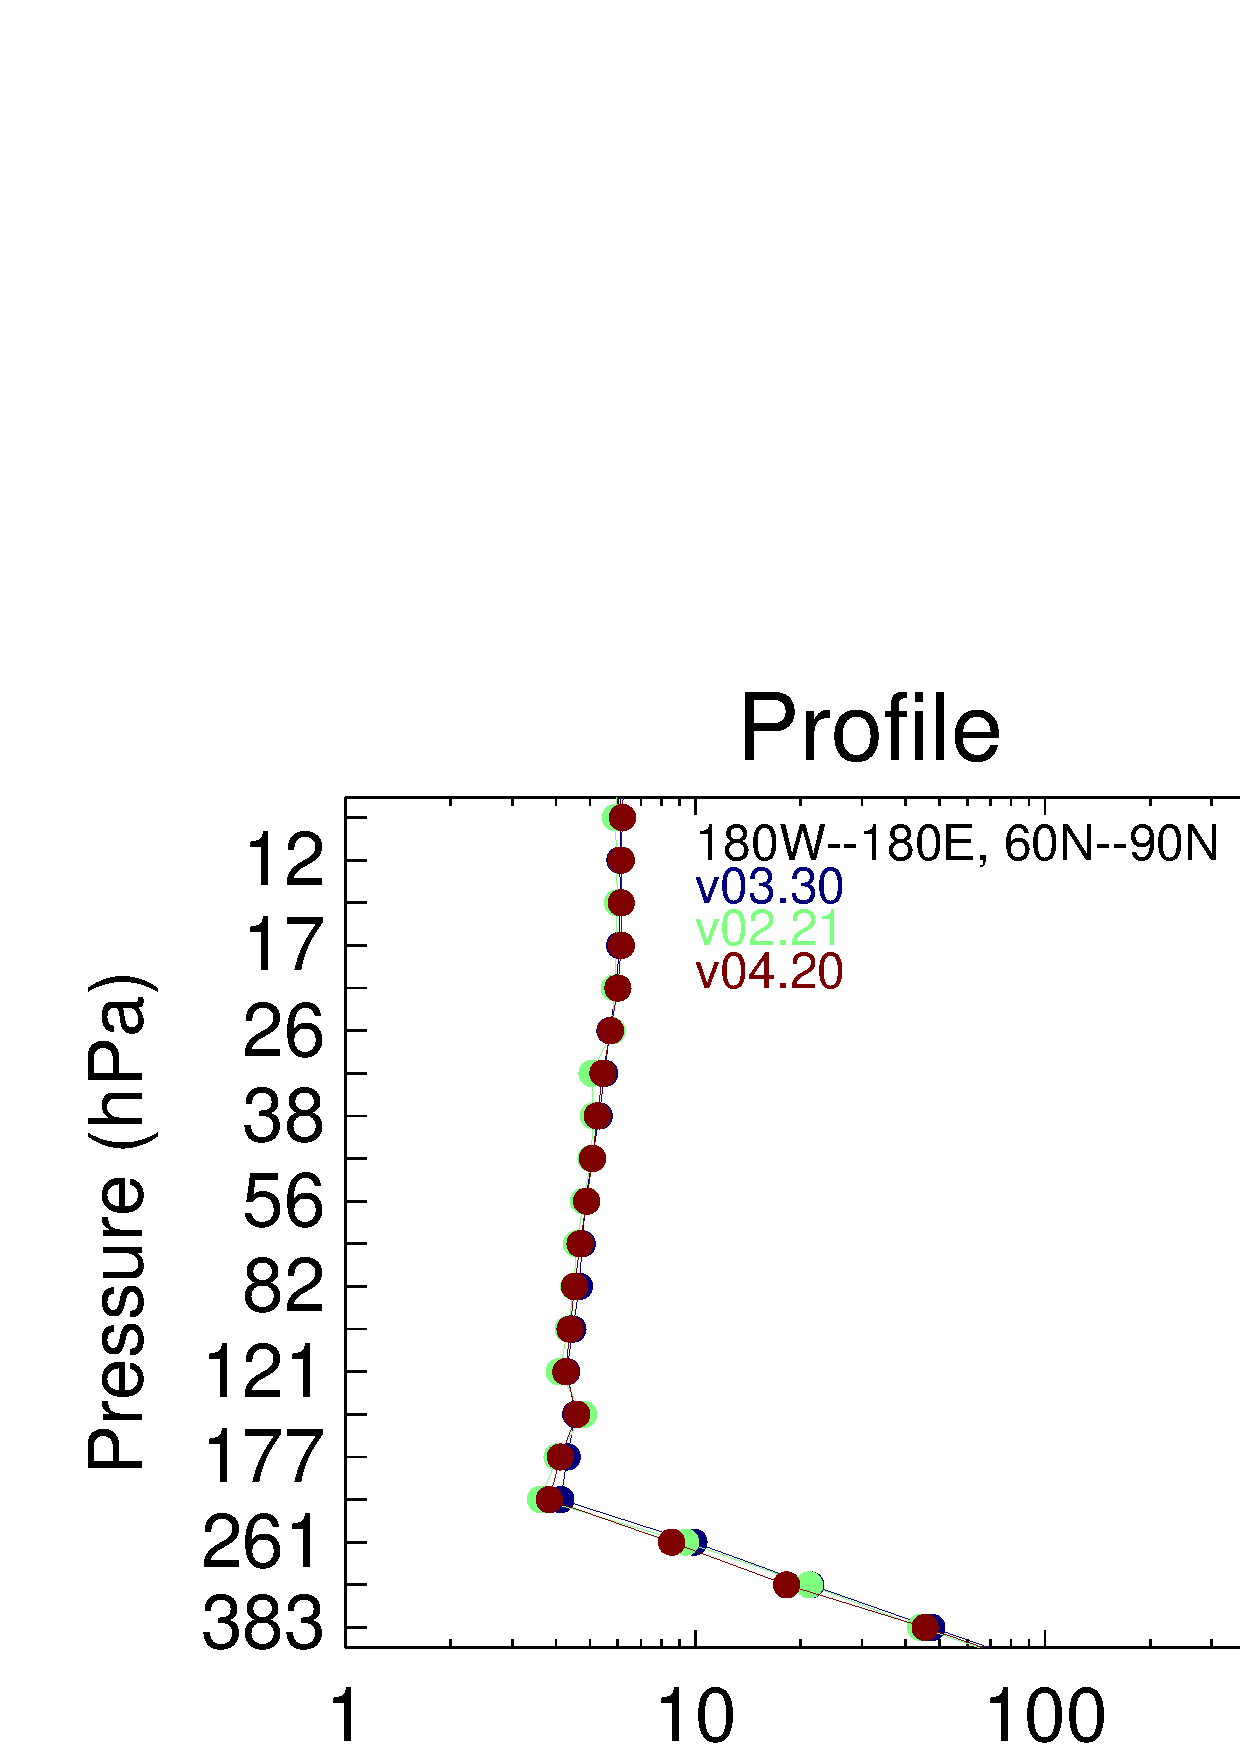
\includegraphics[width=0.8\linewidth]{figures/mls_h2o_v3-v4_prfl_comp_60n-90n}
\includegraphics[width=0.8\linewidth]{figures/mls_h2o_v3-v4_prfl_comp_30n-60n}
\includegraphics[width=0.8\linewidth]{figures/mls_h2o_v3-v4_prfl_comp_30s-30n}
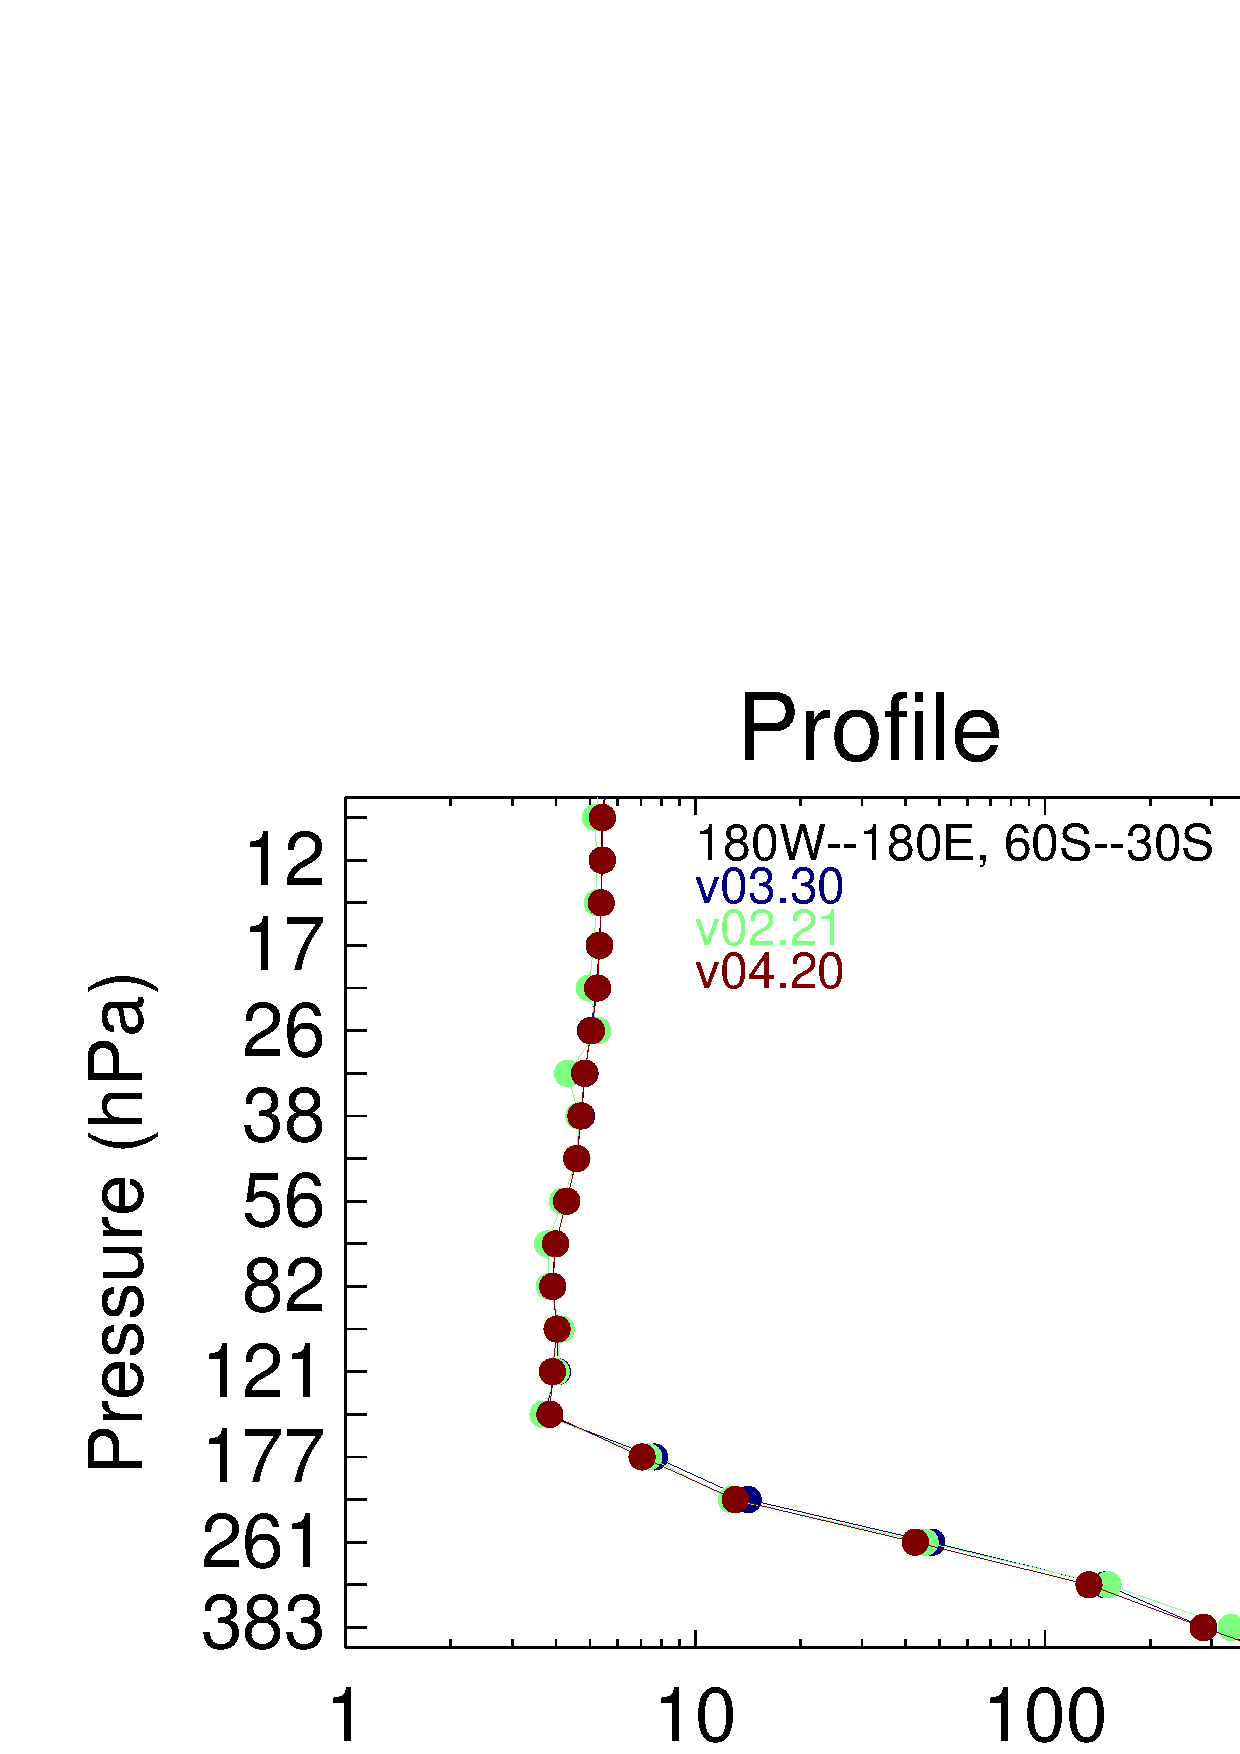
\includegraphics[width=0.8\linewidth]{figures/mls_h2o_v3-v4_prfl_comp_60s-30s}
\includegraphics[width=0.8\linewidth]{figures/mls_h2o_v3-v4_prfl_comp_90s-60s}
\end{center}
\caption{A comparison of \prevvSlash (blue) to v2.2 (green) and \thisv
  (red) water vapor for Jan-Feb-Mar 2005 in 5 latitude bands. Other time
  periods are similar. The left panel compares mean profiles, the center
  shows the mean difference (red and green diamonds) surrounded by each
  version's estimated precision, and the right panel shows the estimated
  retrieval precision (solid and bullets) and measured variability
  (dotted) which includes atmospheric variability about the mean
  profile.}
\label{fig:avgmlsprflcomp}
\end{figure}

Figure~\ref{fig:avgmlsprflcomp} compares MLS \thisv to \prevvSlash and
v2.2. At most levels, the average difference is small -- less than
10\%. The 316\,--\,215-hPa levels are 10\,--\,20\% drier in \thisv than
\prevv. This difference in behavior is replicated in simulation studies
where the agreement with truth is better in \thisv. The extremely low
values of the 215-hPa H\cs2O at high latitudes seen in previous versions
are still present in \thisv. Unfortunately the high latitude behavior is
not replicated in simulation studies and therefore is a systematic error
that is not understood.

Humidity data at pressures greater than 316\,hPa are derived from a
broad layer relative humidity retrieval (using low limb viewing MLS wing
channel radiances) similar to that obtained from NOAA operational
humidity sounders such as TOVS\@. As noted in \citep{ReadEtal07}, the
v2.2 retrieval at pressures larger than 316\,hPa was likely to be
\texttildelow30\% too high, based on comparisons with AIRS\@. The
accuracy of this retrieval is highly sensitive to the transmission
efficiency of the MLS optics system. In \prevv the assumed value of the
MLS antenna transmission efficiency was adjusted empirically (within the
uncertainty range established from MLS calibration) to give better
agreement with AIRS in the tropics. In \thisv the N\cs2 continuum was
adjusted only for this phase to minimize the clear sky cloud induced
radiance bias. This retrieval is used as an \emph{a priori} and profile
constraint for the humidity profile at pressures greater than 316\,hPa,
which are not retrieved in the standard H\cs2O product retrieval.

\sloppypar The third panel in Figure~\ref{fig:avgmlsprflcomp} shows the mean
estimated single profile precision and the measured variability (which
includes instrument noise and atmospheric variability). The precisions
for \thisv and \prevvSlash are nearly identical except for pressures
greater than 68\,hPa where \thisv is producing lower values. Version 2
used a more coarse retrieval grid above 22\,hPa and a different value of
the H\cs2O linewidth.  Together these account for H\cs2O precision
differences at these altitudes between v2 and later versions.

Figures~\ref{fig:avgmlsh2ozmcomp1} and \ref{fig:avgmlsh2ozmcomp2} show a
comparison of H\cs2O zonal means from v2, v3, and v4 retrievals for
100\,--\,2.6\,hPa and 2.2\,--\,0.002-hPa, respectively. Version 4 H\cs2O
tends to show only minor departures from v3. Version 2 H\cs2O shows some
vertical oscillatory behavior at some levels that was removed when an
improved linewidth was used in v3. The latitude structure tends to be
very similar in all cases except at 0.002\,hPa for v2.2.

\begin{figure}
\begin{center}
\includegraphics[width=0.8\linewidth]{figures/InspectZM_2009m03_H2O-v04-2x_H2O-v03-3x_H2O-v02-2x_userHeightRange1}
\end{center}
\caption{A comparison of \thisv (red) to \prevvSlash (blue) and v2.2 (green) water
  vapor zonal means for March 2009. Each panel represents a pressure as
  noted above. The pressures shown range from 100~hPa to 2.6~hPa.}
\label{fig:avgmlsh2ozmcomp1}
\end{figure}

\begin{figure}
\begin{center}
\includegraphics[width=0.8\linewidth]{figures/InspectZM_2009m03_H2O-v04-2x_H2O-v03-3x_H2O-v02-2x_userHeightRange2}
\end{center}
\caption{A comparison of \thisv (red) to \prevvSlash (blue) and v2.2 (green) water
  vapor zonal means for March 2009. Each panel represents a pressure as
  noted above. The pressures shown range from 2.2\,hPa to 0.002\,hPa.}
\label{fig:avgmlsh2ozmcomp2}
\end{figure}

\subsection*{Resolution}
\onestandardavk{H2O_HR}{H\cs2O}%

The spatial resolution is obtained from examination of the averaging
kernel matrices shown in Figure~\ref{fig:AvkH2O_HR}.  The vertical
resolution for H\cs2O is in the range 1.3\,--\,3.6\,km from
316\,--\,0.22\,hPa and degrades to 6\,--\,11\,km for pressures lower
than 0.22\,hPa. The along track horizontal resolution is
\texttildelow170\,--\,350\,km for pressures greater than 4.6\,hPa, and
degrades to 400\,--\,740\,km at smaller pressures. The resolutions in
Table~\ref{tab:H2OSummary} are a smoothed average of the equatorial and
70\degsym N values shown in Figure~\ref{fig:AvkH2O_HR}. The horizontal
cross-track resolution is 7\,km, the width of the MLS 190-GHz
field-of-view for all pressures. The longitudinal separation of the MLS
measurements is 10\degsym\,--\,20\degsym\ over middle and lower
latitudes, with much finer sampling in polar regions.

\subsection*{Precision}

Table~\ref{tab:H2OSummary} summarizes the estimated precision of the MLS
\thisv H\cs2O data. For pressures $\geq100\,\text{hPa}$, the precisions
given are the $1\sigma$ scatter about the mean of coincident comparison
differences, which are larger than the formal retrieval precisions
\citep{ReadEtal07}.  For pressures $\leq$83\,hPa the precisions are the
$1\sigma$ scatter of coincident ascending/descending MLS profile
differences \citep{LambertEtal07}.  The individual Level~2 precisions
are set to negative values or zero in situations when the retrieved
precision is larger than 50\% of the a priori precision -- an indication
that the data are biased toward the a priori value.

\subsection*{Accuracy}

The values for accuracy are based primarily on two sources: comparisons
with validated instruments and a systematic error analysis performed on
the MLS measurement system \citep{ReadEtal07} and \citep{LambertEtal07}
(performed for v2, but expected to be insignificantly different for
H\cs2O in \thisv because the relevant aspects of the instrument's
calibration and spectroscopic uncertainties and the retrieval set up
have not changed. A systematic errors study will be performed on v4
soon).  For pressures between 316\,--\,178\,hPa, Comparisons between
AIRS v6 and MLS \thisv show $<$20\% agreement in the zonal mean (MLS
usually drier for low concentrations and wetter for high concentrations)
equatorward of 40\degsym\ with MLS having large dry biases at higher
latitudes.

The values in Table~\ref{tab:H2OSummary} for pressures between 316 and
178\,hPa are AIRS validated accuracies which are better than those
theoretically possible for the MLS measurement system. For the pressure
range 178\,--\,83\,hPa, the quoted values come directly from the
systematic error analysis performed on the MLS measurement
system. Comparisons between MLS and frost point hygrometers show that,
when the tropopause is between 215 and 147\,hPa, MLS H\cs2O at the
tropopause level tends to have a large (20\,--\,30\%) dry biases.
Future work to understand this behavior is planned.  An estimate of the
accuracy between 121\,--\,83\,hPa is also from the systematic error
analysis performed on the MLS measurement system.  Comparisons among
\emph{in situ} sensors on the WB-57 high altitude aircraft and
frostpoint hygrometers flown on balloons show 30\% disagreements -- well
in excess of the estimated accuracy of each instrument including MLS --
near the tropopause and lower stratosphere.  The balloon based frost
point hygrometer shows agreement better than indicated in
Table~\ref{tab:H2OSummary}. The validation paper describes in detail why
a 30\% spread is inconsistent with the MLS measurements
\citep{ReadEtal07}.  For pressures less than 83\,hPa, the accuracy is
based on the systematic error analysis.

\subsection*{Data screening}
\label{sec:H2OScreening}
\begin{description}
\item[Pressure range:] \screeningrule{316\,--\,0.002\,hPa.}
  \standardrangestatement
\standardprecisionrule
\evenstatusrule
\item[Clouds:] Ignore status bit 16 (high cloud) or bit 32 (low cloud) set
indicating the presence of clouds. See artifacts for more details.
\item[Quality field:] \screeningrule{Only profiles with a value of the
    \texttt{Quality} \emph{greater} than 1.45 should be used in
    scientific studies.}  This recommendation is for scientific studies
  taking advantage of the global and long-temporal characteristics of
  the data and aims to keep the best radiometrically fit data over the
  full retrieval range. Most of the ``badness'' in quality tends to
  affect the lowermost retrieval range of the product (particularly the
  316-hPa level and also where clouds can degrade the fit). Low quality
  values often do not affect the stratospheric and mesospheric part of
  the product and much lower \texttt{Quality} values can be
  tolerated. Figure~\ref{fig:datayields} shows the percentage decline in
  good data yields as a function of quality selected for all 2005
  data. There is a slight seasonal dependence in the function with
  January--February having a 2\% higher yield at \texttt{Quality}$ =
  1.45$.  The recommended \texttt{Quality} threshold value is where the
  function starts to rapidly decline, indicating that well fit data is
  getting rejected. The chosen value will eliminate \texttildelow5\% of
  the profiles on a typical day. One may wish to ignore the
  \texttt{Quality} field for ``process'' studies or situations where a
  small number of profiles are being used, particularly if the
  stratospheric region is being studied. The MLS team should be
  consulted if one wishes to use a few select profiles having a
  \texttt{Quality} less than that recommended to ensure that the product
  is trustworthy.

\item[Convergence field:] \screeningrule{Only profiles with a value of
    the \texttt{Convergence} \emph{less} than 2.0 should be used in
    scientific studies.}
\end{description}

\begin{figure}
\begin{center}
\includegraphics[width=0.8\linewidth]{figures/h2o_data_yields}
\end{center}
\caption{Percentage of data having a quality greater than that indicated
 on the x-axis for \thisv data processed for all of 2005.}
\label{fig:datayields}
\end{figure}

\subsection*{Artifacts}

There is a minimum concentration where MLS H\cs2O measurements become
unreliable. This is given in Table~\ref{tab:H2OSummary} under the ``Min.
H\cs2O'' column. The lowest allowable H\cs2O value is 0.1\,ppmv.
Differences between the retrieved middle tropospheric H\cs2O constraint
and the true atmospheric state can cause errors at 316 and 261\,hPa.
The error manifests either as dry ($<$1\,ppmv) or moist spikes in an
orbital time series. Such data are often accompanied with good quality
and status.

Clouds in the field of view degrade the data in unpredictable ways. Many
instances of quality $<$1.45 occur in the presence of clouds where the
cloud screening has not rejected the radiances. Cloud radiative
scattering distorts the spectral lineshape causing poor fits and low
quality values.  However, not all MLS signals are obviously
affected. Coincident comparisons of MLS cloud flagged H\cs2O
(\texttt{status} bit 16 or 32 set between 316\,--\,215\,hPa) with good
quality AIRS show a small mean bias of 10\% but exhibit a 50\% increase
in variability for the individual differences. Therefore users should be
aware that, although the overall biases for measurements inside clouds
are similar to that for clear sky, individual profiles will exhibit
greater variability about the true atmospheric humidity.

\subsection{A note about the water vapor averaging kernels}

The averaging kernels are most applicable to linear and moderately
non-linear retrieval problems. The MLS H\cs2O retrievals are mostly
linear, except when the atmosphere approaches opaqueness. This occurs
when the limb tangent of the instrument field of view is less than
10\,km above the Earth's surface and the atmosphere is moist.  In such
cases the measurements are very nonlinear and often times the averaging
kernel calculations for the lowest retrieved levels are numerically
unstable, and unrepresentative of the actual MLS measurement system.
This is the case, for example, for the 316-hPa and 262-hPa equatorial
kernels shown in Figure~\ref{fig:AvkH2O_HR}.  Analysis of simulated MLS
observations indicates that application of the averaging kernel provides
little benefit to analyses involving the 316-hPa and 262-hPa levels, and
accordingly we recommend not applying the (unrepresentative) kernels at
those levels.

\subsection*{Review of comparisons with other datasets}

\begin{figure}
\begin{center}
  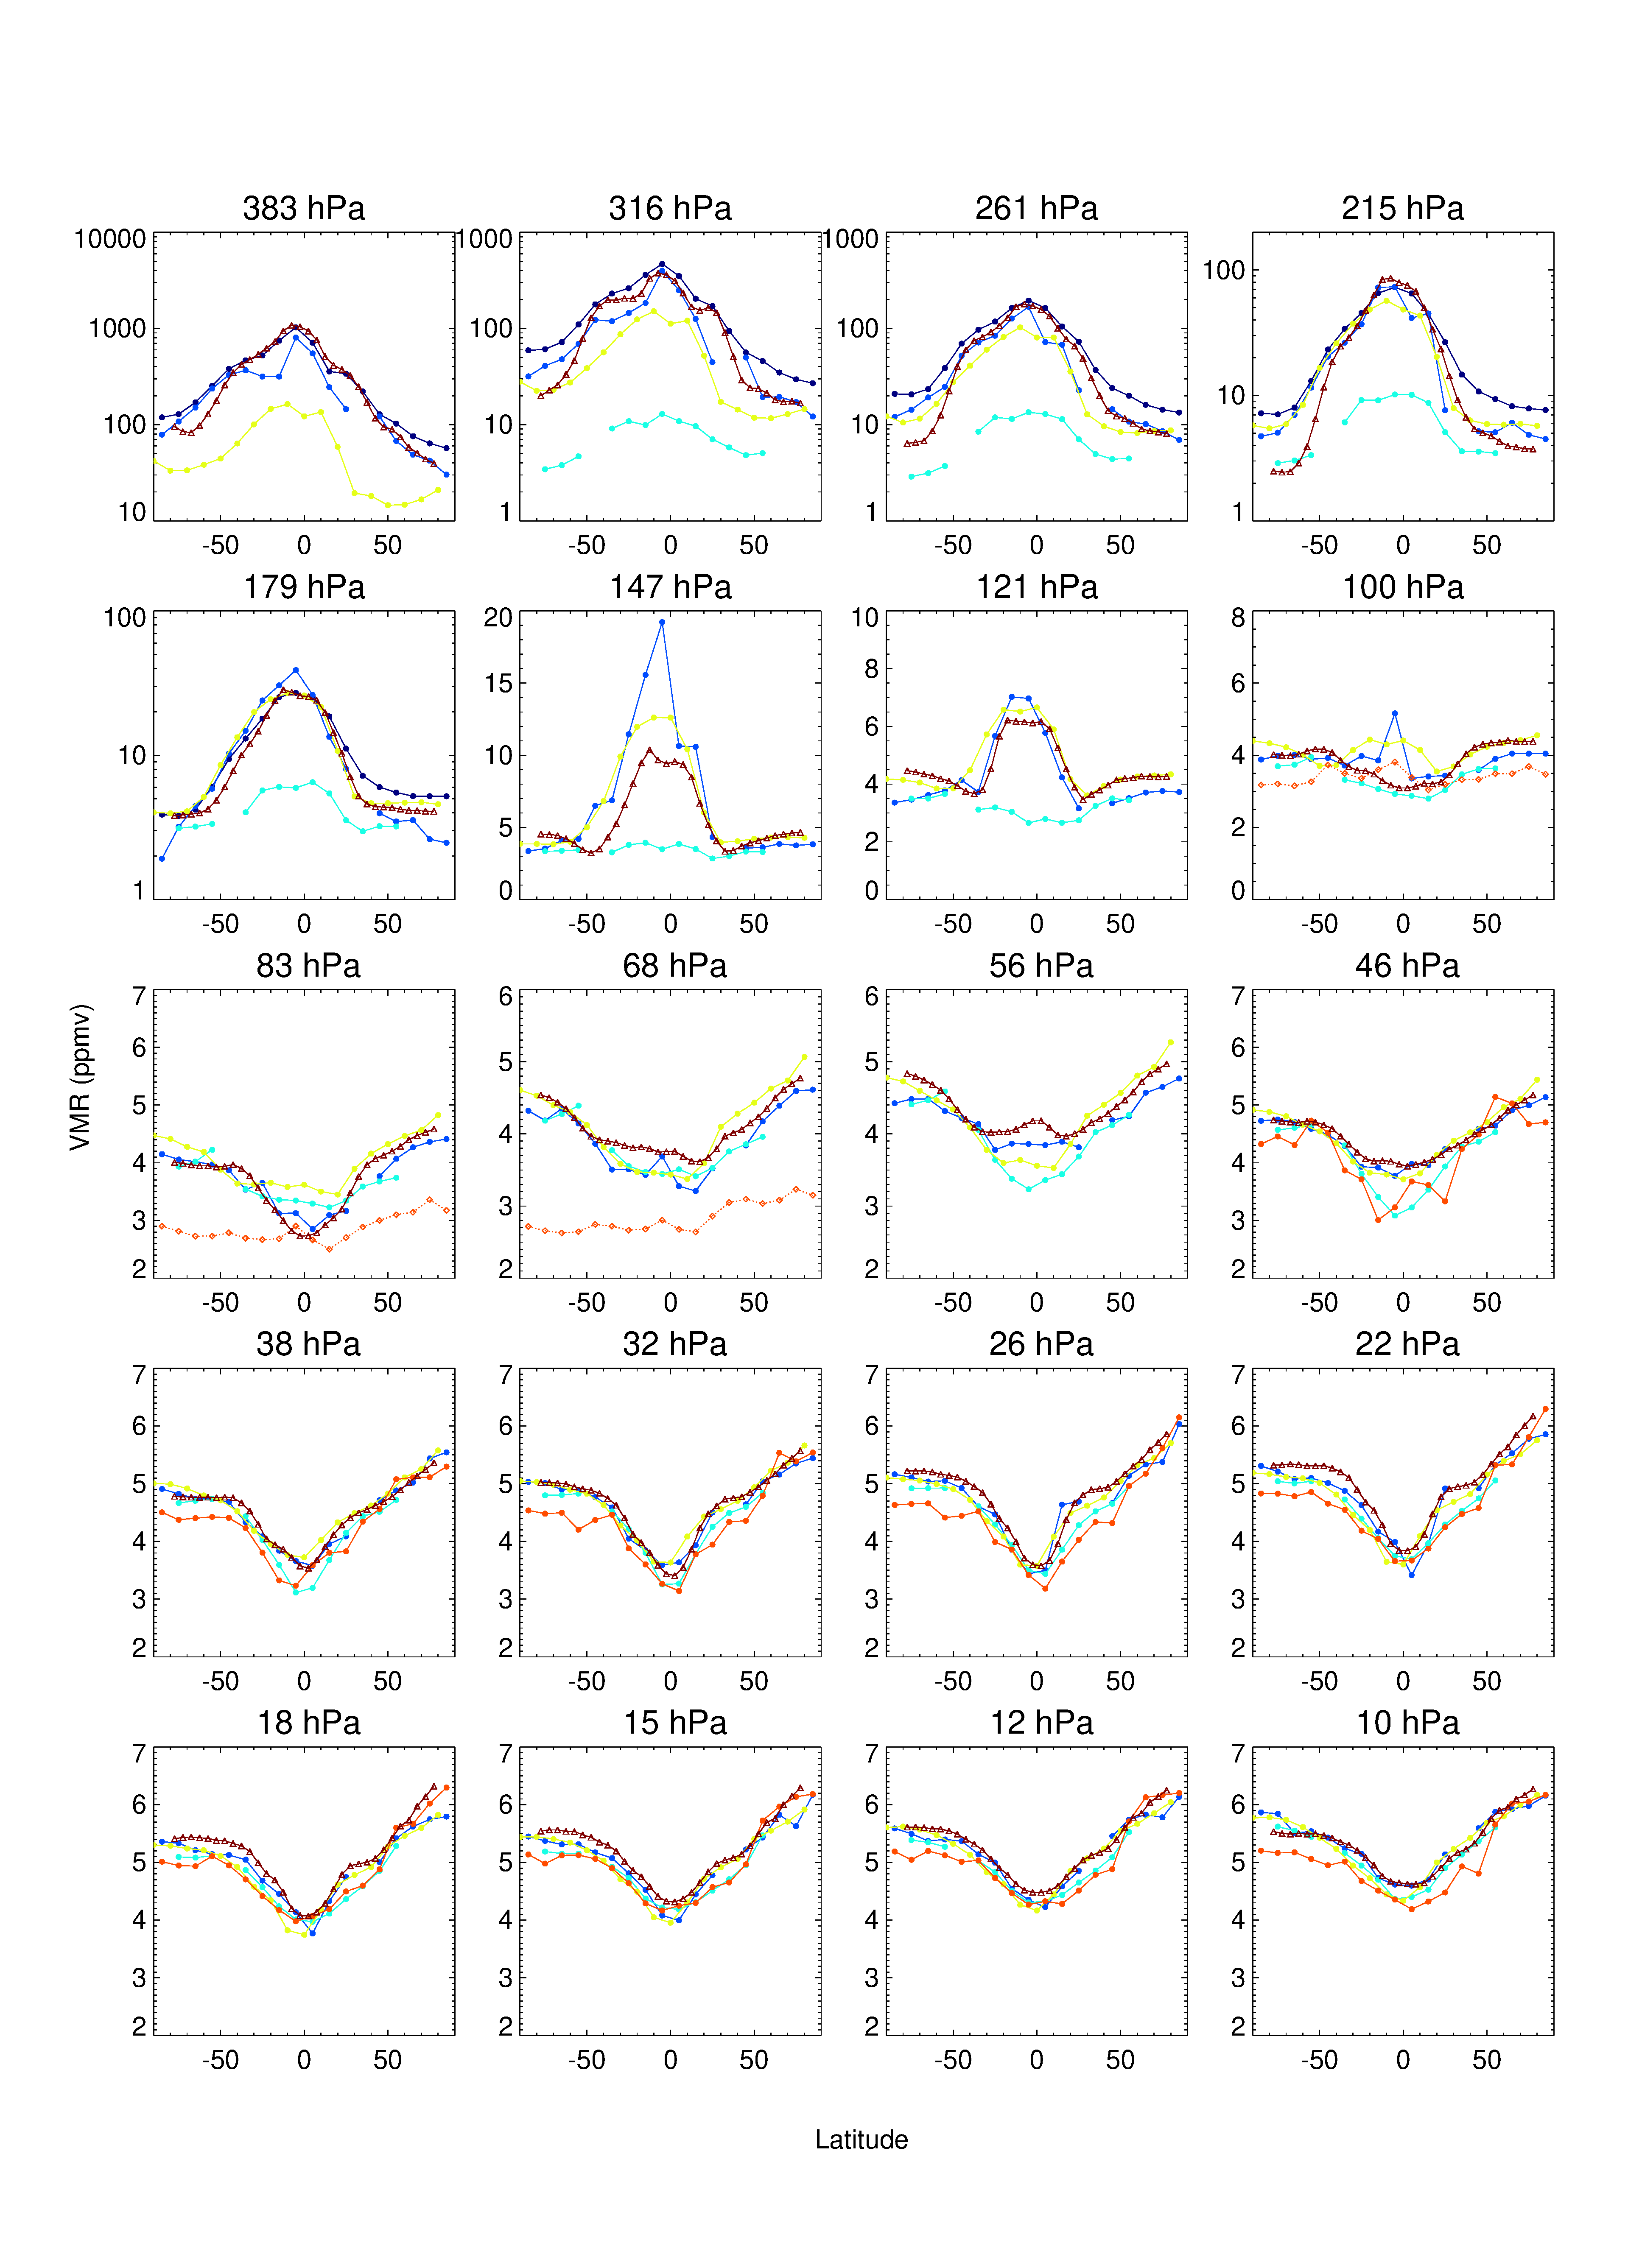
\includegraphics[bb = 58 120 1776 2340, clip,
  width=0.9\linewidth]{figures/sat_h2o_comps}
\end{center}
\caption{A comparison of MLS \thisv (red) water vapor for Jan-Feb-Mar
  2005 with other satellite observations shown as latitude-value zonal
  means. Each panel represents a pressure surface. The satellites are:
  AIRS v6 (dark blue), ACE-FTS v3.5 (light blue), MIPAS IMK v4
  (yellow-green), HALOE v19 (cyan), Odin SMR 544 GHz continuum product
  (orange open diamonds), and Odin SMR line resolved product (orange
  solid bullets).}
\label{fig:satcomps}
\end{figure}

Figure~\ref{fig:satcomps} shows a latitude-value zonal mean comparison
among several satellite data sets. The satellite datasets include MLS
\thisv, AIRS v6, ACE-FTS v3.5, MIPAS IMK v4, HALOE v19, Odin SMR
continuum H\cs2O, and Odin SMR line resolved H\cs2O. ACE-FTS and MLS
show the best agreement with each other throughout the full vertical
range and over most latitudes. MLS also agrees well with AIRS v6 over
the lower latitudes. MLS however does have a significant dry bias at
high latitudes which is often a factor of two. MIPAS-IMK at most
altitudes and latitudes show similar behavior to MLS except near the
cold point tropopause where MLS shows lower values in the tropics
whereas MIPAS does not. HALOE is much too dry in the tropics but behaves
like MLS for pressures $\le 100\,\text{hPa}$.  The Odin SMR continuum
product (100--68 hPa) does not agree well with the other satellite based
products. The Odin-SMR line resolved product (pressures less than or
equal to 46\,hPa) usually agrees within 10\% of MLS v4 for all heights
and latitudes.

One potential improvement in \thisv is shown in
Figures~\ref{fig:airsmlsjf2005maps} and \ref{fig:airsmlsjja2005maps}
that compare multi-month maps of MLS with AIRS v6. The very moist
regions over the tropics in v4 have become a bit drier and in better
agreement with AIRS.

\begin{figure}
\begin{center}
  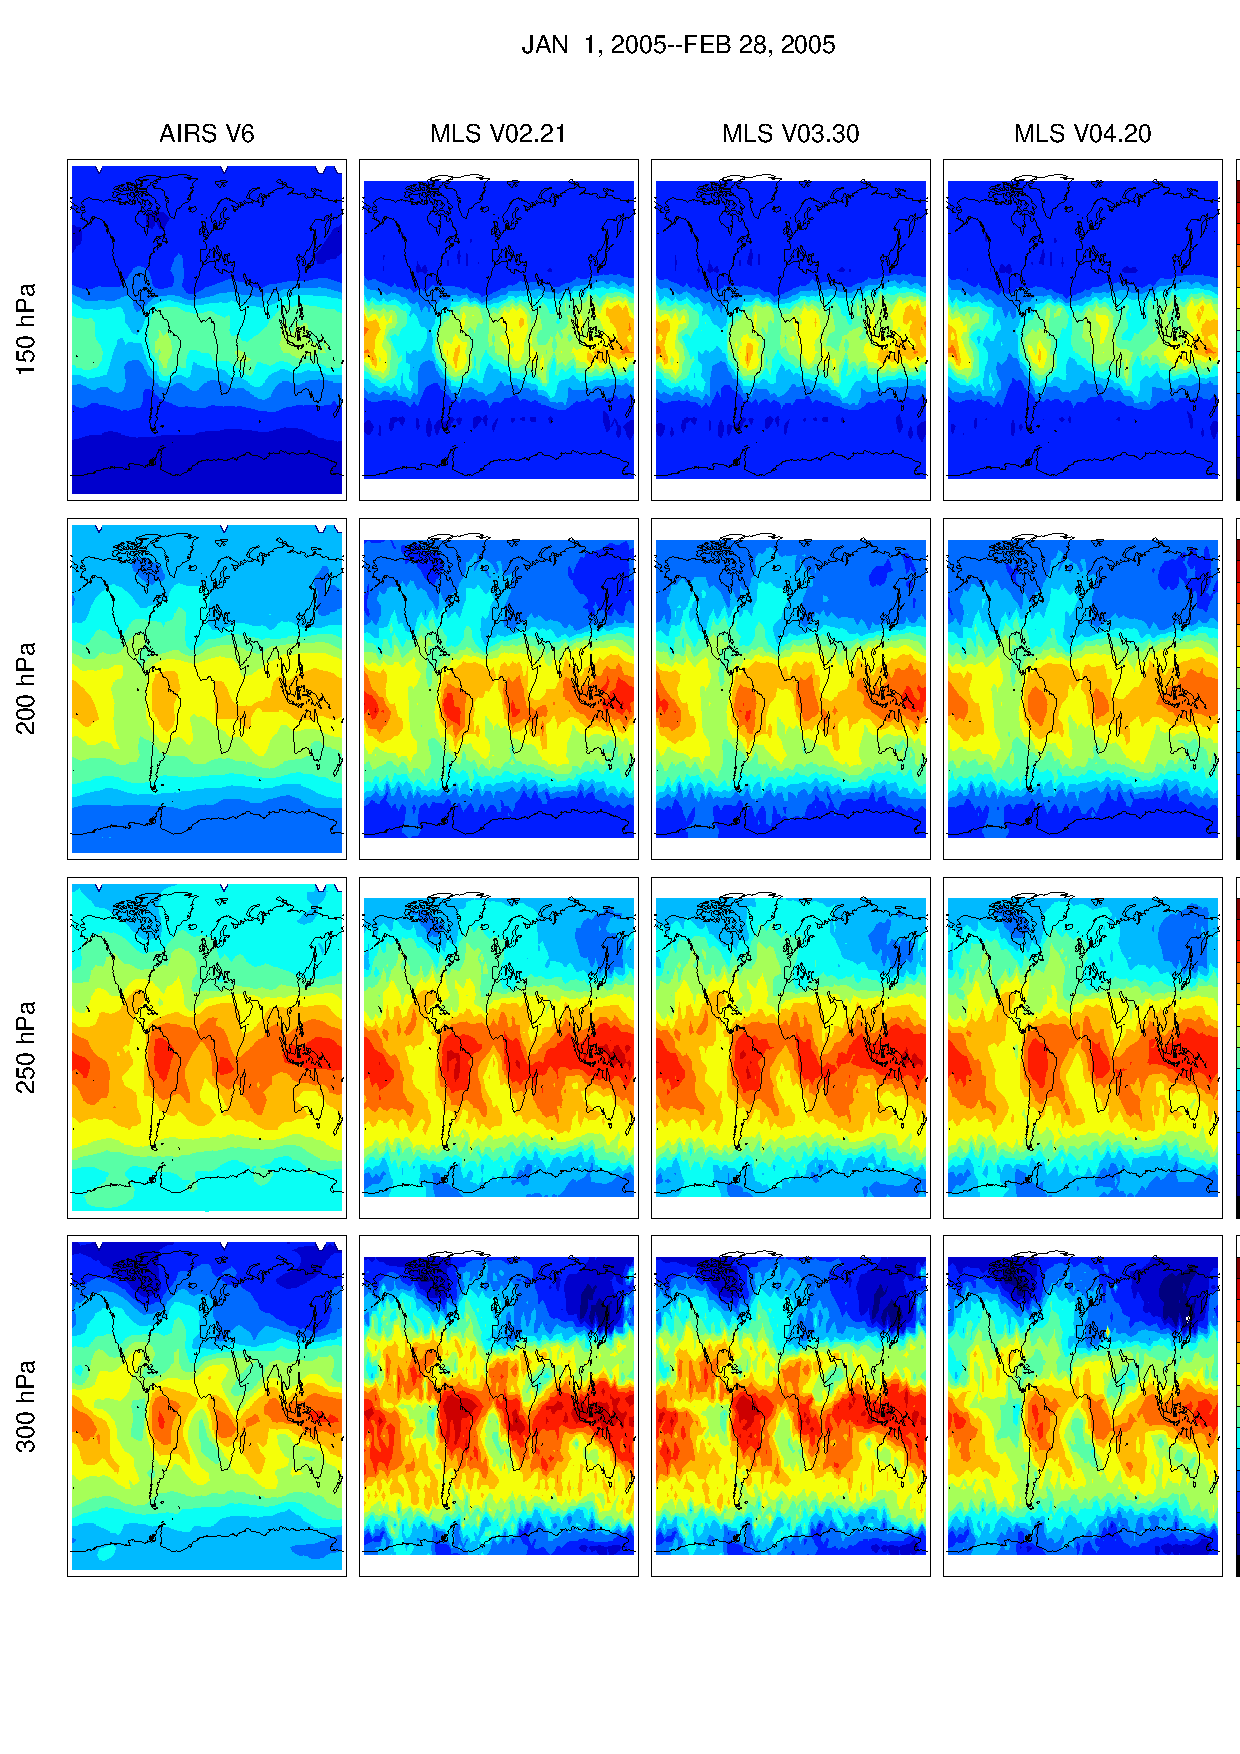
\includegraphics[width=0.9\linewidth]
{figures/grid_maps_jf2005_airsv6-mlsv3andv4}
\end{center}
\caption{Mapped fields from AIRS v6 (left), MLS v2.2 (center-left), MLS
  \prevvSlash (center-right), and MLS \thisv (right) pressures between
  300--150\,hPa for January and February 2005. Note that the AIRS
  measurement is mostly suitable for H\cs2O greater than 10\,ppmv.}
\label{fig:airsmlsjf2005maps}
\end{figure}

\begin{figure}
\begin{center}
  \includegraphics[width=0.9\linewidth]
{figures/grid_maps_jja2005_airsv6-mlsv3andv4}
\end{center}
\caption{Mapped fields from AIRS v6 (left), MLS v2.2 (center-left), MLS
  \prevvSlash (center-right), and MLS \thisv (right) pressures between
  300\,--\,150 hPa for June through August 2005. Note that the AIRS
  measurement is mostly suitable for H\cs2O greater than 10\,ppmv.}
\label{fig:airsmlsjja2005maps}
\end{figure}


Apart from the differences noted above, the MLS \thisv H\cs2O is similar
to the MLS \prevvSlash and MLS v2.2 products, the latter described and
validated in \citet{ReadEtal07} and \citet{LambertEtal07}. The H\cs2O
validation paper used AIRS v4 and MLS v2 humidities and both of them
have become more dry in their subsequent versions. A revised validation
paper for H\cs2O is not planned in the near future and users are
encouraged to read \citet{ReadEtal07} and \citet{LambertEtal07} for more
information. MLS \prevvSlash is a part of a satellite H\cs2O assessment
report to be published later this year.

\subsection*{Desired improvements for future data version(s)}

We want to improve high latitude performance of 261 and 215~hPa H\cs2O
in future work. Possibly a vertically resolved H\cs2O product for
pressure $>316\,\text{hPa}$ at high latitudes during dry conditions.

\begin{table}
\caption{Summary of MLS \thisv H\cs2O product.}
\vspace{\tablecaptionsep}
\label{tab:H2OSummary}
\begin{minipage}{\linewidth}
\centering\begin{tabular}{cccccm{30ex}}
\toprule
\parbox{10ex}{\centering\bfseries Pressure / hPa} &
\parbox{11ex}{\centering\bfseries Resolution V$\times$H / km} &
\parbox{10ex}{\centering\bfseries Precision\footnote{Precision for a
    single MLS profile} / \%} &
\parbox{10ex}{\centering\bfseries Accuracy / \%} &
\parbox{10ex}{\centering\bfseries Min. / ppmv\footnote{Minimum H\cs2O is an estimate of the minimum H\cs2O 
concentration measurable by \thisv MLS.}} &
\parbox{11ex}{\centering\bfseries Comments} \\
\midrule
$\le$0.001  & --- & --- & --- & --- & Unsuitable for scientific use \\
0.002 & 10.3 $\times$ 350 &152 & 34 & 0.1 & \\
0.004 & 10.8 $\times$ 585 & 81 & 16 & 0.1 & \\
0.010 &  8.8 $\times$ 725 & 55 & 11 & 0.1 & \\
0.021 &  8.0 $\times$ 745 & 41 &  9 & 0.1 & \\
0.046 &  7.4 $\times$ 540 & 35 &  8 & 0.1 & \\
0.10 &  5.8 $\times$ 745 & 24 &  8 & 0.1 & \\
0.21 &  3.6 $\times$ 670 & 19 &  7 & 0.1 & \\
0.46 &  3.3 $\times$ 505 & 12 &  6 & 0.1 & \\
1.0 &  2.5 $\times$ 400 &  6 &  4 & 0.1 & \\
2.2 &  3.5 $\times$ 385 &  4 &  5 & 0.1 & \\
4.6 &  3.4 $\times$ 350 &  4 &  7 & 0.1 & \\
10 &  2.8 $\times$ 290 &  6 &  9 & 0.1 & \\
22 &  3.2 $\times$ 265 &  5 &  7 & 0.1 & \\
46 &  3.2 $\times$ 230 &  5 &  4 & 0.1 & \\
68 &  3.1 $\times$ 190 &  5 &  6 & 0.1 & \\
83 &  3.1 $\times$ 190 &  7 &  7 & 0.1 & \\
100 & 3.0 $\times$ 198 & 15 &  8 & 0.1 & \\
121 & 2.6 $\times$ 193 & 20 & 12 & 0.1 & \\
147 & 2.3 $\times$ 188 & 20 & 15 & 0.1 & \\
178 & 1.7 $\times$ 183 & 25 & 20 & 3   & \\
\addlinespace
215 & 1.6 $\times$ 178 & 40  & 25 &  3   & Large low bias for latitudes
$>60\degsym$ \\
\addlinespace
261 & 1.4 $\times$ 173 & 35  & 20 &  4   & Large low bias for latitudes
$>60\degsym$ \\
\addlinespace
316 & 1.3 $\times$ 168 & 65  & 15 &  7   & Occasionally erroneous low value
$<1\,\text{ppmv}$ and high value fliers are retrieved in the tropics, usually in
clouds. \\
\addlinespace
$>316$ & --- & --- & --- & --- & Unsuitable for scientific use \\
\bottomrule
\end{tabular}
\end{minipage}
\end{table}


%%% Local Variables: 
%%% mode: latex
%%% TeX-master: "v4-x-report"
%%% End: 
 <\speciestitle{Hydrogen Chloride}{HCl}{HCl}{%
\item[Useful range:] 100\,--\,0.32\,hPa 
\item[Contact:] Lucien Froidevaux,
  \email{Lucien.Froidevaux@jpl.nasa.gov}}

\subsection*{Introduction}

There has been very little change in the v4.2 HCl retrieval results, in
comparison to v3.3/v3.4. We provide below sample mean HCl distributions
for the two data versions, and their differences. Otherwise, previous
information regarding this species remains largely unchanged; the main
points are mentioned here mainly for new data users.

The MLS v3.3/v3.4 retrievals of the HCl standard product (from the
640\,GHz radiometer) use channels from band 14, as a result of the
deterioration observed since early 2006 in nearby band 13, originally
targeted (with narrower channels than band 14) at the main HCl emission
line center. Full measurement days with band 13 on after February 15,
2006, are as follows: March 15, 2006 (2006d074), April 14, 2006
(2006d104), January 6 through 8, 2009 (2009d006 through 2009d008), and
January 24 through 27, 2010 (2010d024 through 2010d027).  For days prior
to February 16, 2006 and for the few days (as listed above) when band 13
gets turned on thereafter, the MLS Level~2 software also produces a
separate \texttt{HCl-640-B13} product (stored in the \texttt{L2GP-DGG}
file), using the band 13 radiances.  This product has slightly better
precision and vertical resolution in the upper stratosphere than the
standard HCl product.  The MLS team plans to turn band 13 on very
infrequently (possibly only one more time), as its lifetime is estimated
at a few days to a few weeks at most, based on the channel counts and
channel noise characteristics observed during the 3-day turn-on period
in late January, 2010; band 13 should provide useful trend information
for upper stratospheric data, given its narrower channels.  Upper
stratospheric trends from the (uninterrupted from 2004 to present) band
14 retrievals are not reliable enough and are too small, compared to
band 13 data and expectations, as well as versus ACE-FTS HCl data.
Scientific usage of the MLS standard HCl (band 14) dataset should
therefore be restricted to the lower stratosphere.

\begin{figure}
  \centering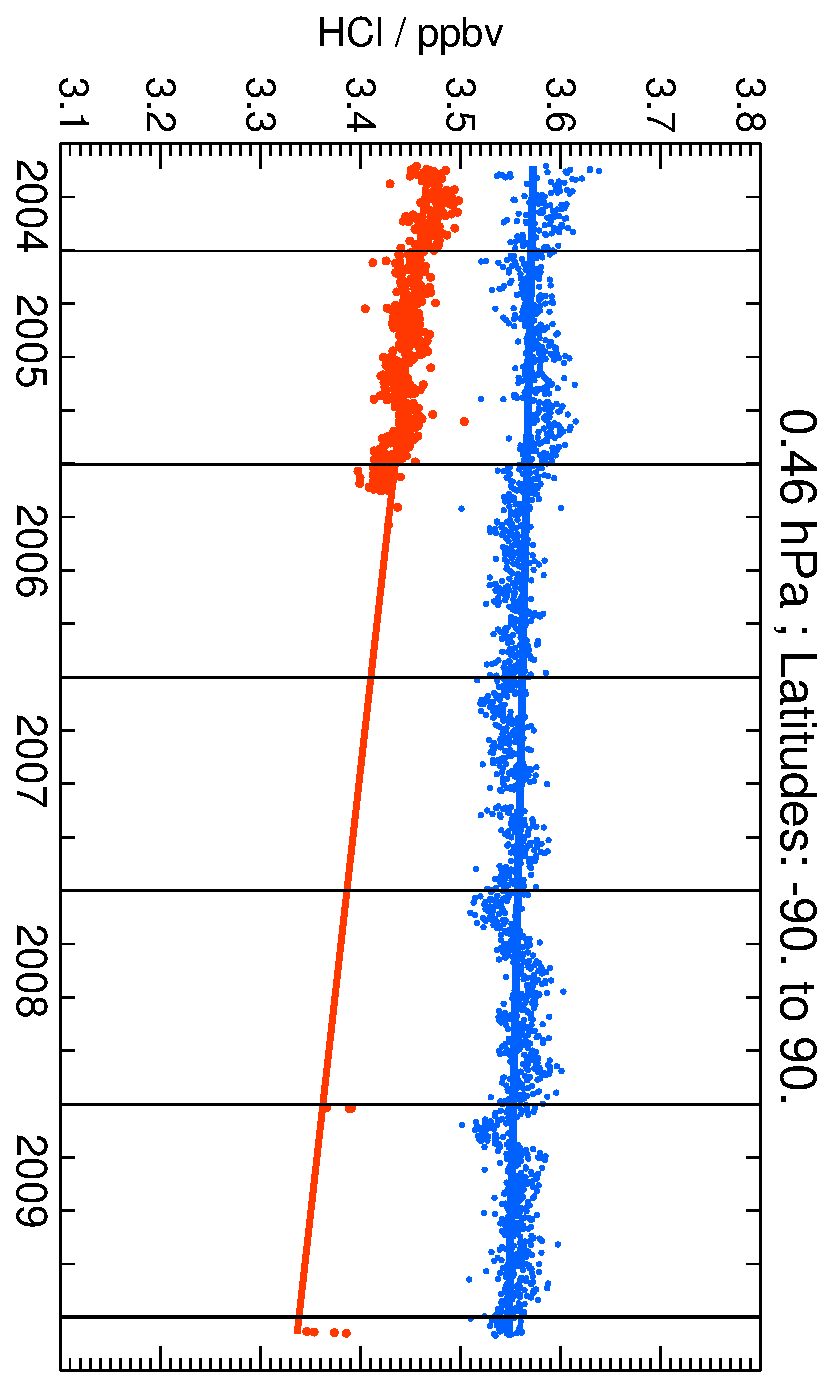
\includegraphics[angle=90,width=0.6\linewidth]{figures/HCl_2bands_0-46hpa_trends_2004_2010}
  \caption{Daily zonal averages for MLS HCl at 0.46\,hPa, from
    mid-August, 2004, through January, 2010, for the originally-targeted
    band 13 measurements (red points), now available only on occasion
    (to preserve lifetime), and the band 14 data (blue points).  The
    lines are simple linear fits through the daily data points; trend
    differences are apparent in this region of the atmosphere, where the
    information obtained from band 14 HCl data is not reliable enough.}
\label{fig:MLSHCl2bands}
\end{figure}


See Figure~\ref{fig:MLSHCl2bands} for an illustration of the trend
differences between these two MLS band measurements of HCl.  In the
lower stratosphere, however, variations in the two HCl products are
closer together, although there is also more seasonal variability; we
believe that the band 14 retrievals are quite appropriate to use in
studies of seasonal (and latitudinal) changes (e.g., during polar
winter/spring), as well as for longer-term trend studies in the lower
stratosphere.

Table~\ref{tab:HClSummary} summarizes the MLS HCl resolution, precision,
and accuracy estimates as a function of pressure.  More discussion and
data screening recommendations for the MLS HCl v4.2 data are provided
below (but this is unchanged from the v3.3/v3.4 recommendations).
Analyses describing detailed validation of the MLS (v2.2) product and
comparisons with other data sets are described in
\citet{FroidevauxEtal08HCl}.  Based on the fairly small overall changes
in v3.3/v3.4 and v4.2 HCl data versus v2.2, the conclusions of the
latter reference should remain essentially unchanged. We also do not
expect the systematic uncertainty estimates in
Table~\ref{tab:HClSummary} to change significantly; however, an MLS team
review of those estimates is pending.

\subsection*{Changes from  v3.3/v3.4}

There were no large algorithmic changes relating to HCl for the v4.2
retrievals. Small differences in HCl abundances (see below) have
occurred mainly near 147\,hPa, most likely mainly as a result of changes
in water vapor in the UTLS.

The background observed in the 640-GHz radiances includes emissions from
N\cs2, O\cs2, and H\cs2O.  There are laboratory-based and ground-based
models for the continuum absorptions that are the basis for the MLS
absorption model [{\it Pardo, 2001}, and references therein].  These
models were tested against MLS extinction measurements from the wing
channels in the 640-GHz radiometer.  The latitude dependence of this
extinction was found to agree better with the expected most plus dry
continuum extinction values if the dry and moist continuum functions
were scaled by factors close to 20\%; however, this is not a change
from the v3.3/v3.4 retrievals.

A comparison plot showing zonal average HCl contours and differences
between the two data versions for a typical month (March, 2009) is
provided in Figure~\ref{fig:MLSv3v4HClContour}.  For pressures larger
than or equal to 0.22\,hPa, the average differences between the two data
versions are typically within 0.1\,ppbv (or 1\,--\,2\%).  The average
changes are easily within the estimated accuracy values (see
Table~\ref{tab:HClSummary}).  The largest percentage changes in HCl
occur for very small mixing ratio values, close to 100 and (mainly)
147\,hPa; v4.2 values are usually smaller than the v3.3/v3.4 values by
10 to 15\% in the lower stratosphere at low latitudes or during winter
at polar latitudes.  There is still, however, an unrealistic high bias
in HCl at 147\,hPa in the tropics, so values at this pressure are not
recommended (reliable in absolute value) within the 40\degsym S to
40\degsym N latitude range. The precisions estimated in the Level~2
files are essentially unchanged from v3.3/v3.4.

\begin{figure}
  \centering\includegraphics[angle=90,width=\linewidth]{figures/Fig-HCl-ZMContours-v3-3-v4-2_2009m03}
  \caption{Zonal averages for MLS HCl profiles during March, 2009,
    showing the MLS v3.3 HCl mixing ratio contours (top left panel), the
    v4.2 contours (top right panel), and their differences in ppbv (v4.2
    minus v3.3, bottom left panel) and percent (v4.2 minus v3.3 versus
    v3.3, bottom right panel).}
\label{fig:MLSv3v4HClContour}
\end{figure}

\subsection*{Resolution}
\onestandardavk{HCl}{HCl}%

Typical (rounded off) values for resolution are provided in
Table~\ref{tab:HClSummary}.  Based on the width of the averaging kernels
shown in Figure~\ref{fig:AvkHCl}, the vertical resolution for the
standard HCl stratospheric product is \texttildelow3\,km (2.7\,km at
best in the lower stratosphere), or about double the 640-GHz radiometer
vertical field of view width at half-maximum; the vertical resolution
degrades to 4--6\,km in the lower mesosphere.  The along-track
resolution is \texttildelow200 to 350\,km for pressures of 2\,hPa or
more, and \texttildelow500\,km in the lower mesosphere.  The cross-track
resolution is set by the 3\,km width of the MLS 640-GHz field of view.
The longitudinal separation of MLS measurements, set by the Aura orbit,
is 10\degsym\,--\,20\degsym\ over middle and lower latitudes, with much
finer sampling in polar regions.

\subsection*{Precision}

The estimated single-profile precision reported by the Level~2 software
varies from \texttildelow0.2 to 0.6\,ppbv in the stratosphere (see
Table~\ref{tab:HClSummary}), with poorer precision obtained in the lower
mesosphere.  These precision values have not changed significantly for
\thisv data.  The Level~2 precision values are often only slightly lower
than the observed scatter in the data, as evaluated from a narrow
latitude band centered around the equator where atmospheric variability
is often smaller than elsewhere, or as obtained from a comparison
between ascending and descending coincident MLS profiles.  The scatter
in MLS data and in simulated MLS retrievals (using noise-free radiances)
becomes smaller than the theoretical precision (given in the Level~2
files) in the upper stratosphere and mesosphere, where there is a larger
impact of \emph{a priori} and smoothing constraints.  The HCl precision
values increase rapidly at pressures less than 0.2\,hPa, and are
generally flagged negative (or zero) at pressures less than 0.1\,hPa;
this indicates an increasing influence from the \emph{a priori} (with
poorer measurement sensitivity and reliability).

\subsection*{Accuracy}

The accuracy estimates in the Table came from a quantification of the
combined effects of possible systematic errors in MLS calibration,
spectroscopy, etc.\ on the HCl retrievals.  These values are intended to
represent $2\sigma$ estimates of accuracy.  For more details, see the
MLS validation paper by \citet{FroidevauxEtal08HCl}.  For \thisv (as for
\prevv), given the trend issues affecting the (band 14) standard HCl
product in the upper stratosphere and lower mesosphere, we have
recommended an accuracy estimate of 10\% in this region (or about
0.3\,ppbv).  Given the agreement between the two bands' retrievals in
the lower stratosphere, we maintain the formal accuracy estimates in
this region (see Table~\ref{tab:HClSummary}).

\subsection*{Data screening}
\label{sec:HClScreening}
\begin{description}
\item[Pressure range:] \screeningrule{100\,--\,0.32\,hPa}
  \standardrangestatement\ We note that the MLS values at 147\,hPa are
  biased high, at least at low to mid-latitudes -- and these values are
  not recommended (particularly equatorward of about 40\degsym). Also,
  although the vertical range at the top end is recommended up to
  0.32\,hPa, users should note the significant issues relating to HCl
  trend estimates in the upper stratosphere and lower mesosphere;
  average profiles in this region can be used for studies not involving
  trends (or accuracy requirements not as tight as 10$\%$).

\standardprecisionrule
\evenstatusrule
\item[Quality field:] \screeningrule{Only profiles with a value of the
    \texttt{Quality} field \emph{greater} than 1.2 should be used.} This
  criterion removes profiles with the poorest radiance fits, typically
  less than 0.1\% of the daily profiles. For HCl (and for other 640\,GHz
  MLS products), this screening correlates well with the poorly
  converged sets of profiles (see below); we recommend the use of both
  the \texttt{Quality} and \texttt{Convergence} fields for data
  screening.

\item[Convergence field:] \screeningrule{Only profiles with a value of
    the \texttt{Convergence} field \emph{less} than 1.05 should be
    used.}  For the vast majority of profiles (99\% or more for most
  days), this field is less than 1.05.  Nevertheless, on occasion, sets
  of profiles (typically one or more groups of ten profiles, retrieved
  as a ``chunk'') have this \texttt{Convergence} field set to larger
  values, and should be discarded.
\end{description}

\subsection*{Review of comparisons with other datasets}

\citet{FroidevauxEtal08HCl} provided results of generally good
comparisons between MLS HCl and other satellite, balloon, and aircraft
measurements.  Both MLS and ACE-FTS HCl values are generally larger (by
about 10\,--\,15\%) than the HCl values from HALOE, especially at upper
stratospheric altitudes; this feature has not changed, overall, with the
new data version(s) from both MLS and ACE-FTS.  MLS HCl at 147\,hPa is
biased high versus WB-57 aircraft in-situ (CIMS) measurements (low to
mid-latitudes); while this is still true for v4.2 data, MLS data at this
pressure level are potentially useful and accurate enough at high
latitudes.

\subsection*{Artifacts}
\begin{itemize} 
\item We do not recommend the use of the MLS HCl standard product (from
  band 14) in the upper stratosphere and lower mesosphere, in terms of
  detailed trend studies, for reasons mentioned above.
\item The HCl values at 147\,hPa are biased high and generally not
  usable (except possibly at high latitudes).  Please consult the MLS
  team for further information.
\item Users should screen out the non-converged and poorest quality HCl
  profiles, as such profiles (typically less than 0.1\% of the data)
  tend to behave unlike the majority of the other MLS retrievals.  See
  the criteria listed above.
\end{itemize}  

\begin{table}
\caption{Summary for MLS hydrogen chloride}
\vspace{\tablecaptionsep}
\label{tab:HClSummary}
\begin{minipage}{\linewidth}\small
\centering\begin{tabular}{ccccccm{25ex}}
\toprule
\parbox[m]{15mm}{\centering\textbf{Pressure}} &
\multicolumn{2}{c}{\parbox[m]{15mm}{\centering\textbf{Precision
      \footnote{Precision ($1\sigma$) for individual profiles; note that
        $\%$ values tend to vary strongly with latitude in the
        lower stratosphere.}}}} &
\parbox[m]{24mm}{\centering\textbf{Resolution\\ V $\times$ H}} &
\multicolumn{2}{c}{\parbox[m]{15mm}{\centering\textbf{Accuracy%
      \footnote{$2\sigma$ estimate from systematic uncertainty
        characterization tests (but see text for estimates at 
        pressures lower than 10\,hPa); note that percent values tend 
        to vary strongly with latitude and season in the lower 
        stratosphere, due to the variability in HCl.}\\}}} 
&
\textbf{Comments} \\
\textbf{hPa} & \textbf{ppbv} & \textbf{\%} & \textbf{km} & \textbf{ppbv} & \textbf{\%} & \\
\midrule
0.22\,--\,0.001 & --- & ---             & ---              & ---   & ---     & Unsuitable for scientific use \\  
0.32            & 0.8 &   25            &   5 $\times$ 450 & 0.3   &  10     & Unsuitable for trend studies \\
0.5             & 0.7 &   20            &   5 $\times$ 400 & 0.3   &  10     & Unsuitable for trend studies \\
1               & 0.5 &   15            &   4 $\times$ 300 & 0.3   &  10     & Unsuitable for trend studies \\
2               & 0.4 &   15            &   3 $\times$ 250 & 0.3   &  10     & Unsuitable for trend studies \\
5               & 0.3 &   10            &   3 $\times$ 200 & 0.3   &  10     & Unsuitable for trend studies \\
10              & 0.2 &   10            &   3 $\times$ 200 & 0.2   &  10     & \\
20              & 0.2 &   15            &   3 $\times$ 200 & 0.1   &  10     & \\
46              & 0.2 & 10 to $>$ 40    &   3 $\times$ 250 & 0.2   &  10 to $>$ 40  & \\
68              & 0.2 & 15 to $>$ 80    &   3 $\times$ 300 & 0.2   &  10 to $>$ 80   &  \\
100             & 0.3 & 30 to $>$ 100   &   3 $\times$ 350 & 0.15  &  10 to $>$ 100  &  \\
147             & 0.4 & 50 to $>$ 100   &   3 $\times$ 400 & 0.3  &   50 to $>$ 100  & High bias at low lats. (use with caution elsewhere) \\  
1000\,--\,215   & --- & ---             & ---              & ---   & ---     & Unsuitable for scientific use \\  
\bottomrule
\end{tabular}
\end{minipage} 
\end{table}

%%% Local Variables: 
%%% mode: latex
%%% TeX-master: "v4-x-report"
%%% End: 
 \speciestitle{Hydrogen Cyanide}{HCN}{HCN}{%
\item[Useful range:] 21\,--\,0.1\,hPa
\item[Contact:] Hugh C. Pumphrey,
  \email{Hugh.Pumphrey@ed.ac.uk}}

\subsection*{Introduction}

HCN is retrieved from bands encompassing, in the lower sideband, the
177.26 GHz spectral line of HCN\@. Although the target line is in an
uncluttered part of the spectrum, the upper sideband contains many
interfering lines of O\cs3 and HNO\cs3. As a result, the \thisv HCN product is
not recommended for general use in the lower stratosphere. In the
recommended range it is usable, but has rather poor precision and
resolution.

It is possible to retrieve weekly zonal means of HCN over a greater
vertical range by first averaging the radiances. Results of this
process and further information on the HCN measurement may be found in
\cite{PumphreyEtal06}.

\subsection*{Differences between v3.x and \thisv}

No changes specific to the HCN retrieval were made between v2.x and v3.x. For
\thisv a new phase was introduced in which HCN is retrieved using only 
bands 6 and 27, rather than all of R2. The \thisv HCN still has
obvious biases in the lower stratosphere, but they are less severe
than in previous versions. As a result, the lowest recommended level
is now 21\,hPa rather than the 10\,hPa recommended for earlier versions.

Figure~\ref{fig:HCNPrecision} shows that the precisions in \thisv are
essentially unchanged from earlier versions. The retrieved mixing
ratios change very little in the region where use was recommended for
earlier versions. Mixing ratios are considerably different between all
three versions in the lower stratosphere where the data are not
recommended for general use. However, the values in \thisv appear less
unrealistic than in either v2.x or v3.x.

\subsection*{Vertical resolution}
\onestandardavk{HCN}{HCN}%

The HCN signal is rather small, so a rather strong smoothing constraint
has to be applied to ensure that the retrieval is at all useful. As
Figure~\ref{fig:AvkHCN} shows, the vertical resolution is about
8\,km at 10\,hPa, degrading to 12\,km at 0.1\,hPa. The horizontal
resolution along the measurement track is between 2 and 4 profile
spacings.

\subsection*{Precision}

Figure~\ref{fig:HCNPrecision} shows the estimated precision (values of
the field {\tt L2gpPrecision}), together with the observed standard
deviation in an equatorial latitude band where the natural variability
of the atmosphere is small. The observed scatter is smaller than the
estimated precision due to the effects of retrieval smoothing.

\begin{figure}
\centering%
\includegraphics[width=0.495\textwidth]{figures/hcn-prec-fig-2005d028}\hfill%
\includegraphics[width=0.495\textwidth]{figures/hcn-prec-fig-2006d059}
\caption{Estimated precision {\tt L2gpPrecision} and observed standard
  deviation for MLS \thisv (black), v3.x (blue) and v2.x (red)
  HCN\@. The data shown are all profiles within 20\degsym\ of the
  equator for 28 January, 2005 and 28 February 2006. Mean mixing ratio
  (VMR) profiles are shown for comparison. Note that these are
  essentially the same in v2.x, v3.x and \thisv for the region
  recommended for use in all three versions(10\,hPa - 0.1\,hPa).}
\label{fig:HCNPrecision}
\end{figure}

\subsection*{Accuracy}

The accuracy of the HCN product has not been assessed in detail
because a cursory inspection revealed that previous versions of the
product had extremely large systematic errors in the lower
stratosphere. These errors are smaller in \thisv, but remain present and
un-quantified.  For this reason the data are not considered to be useful
at pressures greater than 21\,hPa (altitudes
below \texttildelow27\,km).  In the upper stratosphere the values are
in line with current understanding of the chemistry of HCN\@.
Comparison to historical values suggests an accuracy of no worse than
50\%. The precision, resolution and accuracy of the HCN data are
summarized in table~\ref{tab:HCNSummary}.

\begin{table}
  \caption{Summary of data quality for MLS \thisv HCN\@. The precision shown
    is the estimated precision (\texttt{L2gpPrecision}); the observed
    scatter is about 80\% of this value.}
  \vspace{\tablecaptionsep}
\label{tab:HCNSummary}
\centering\begin{tabular}{ccccm{25ex}}
  \toprule
  \parbox{10ex}{\bfseries\centering Pressure} &
  \parbox{11ex}{\bfseries\centering Resolution \mbox{V $\times$ H} / km} &
  \parbox{10ex}{\bfseries\centering Precision / pptv} &
  \parbox{10ex}{\bfseries\centering Accuracy / \%} &
  \parbox{12ex}{\bfseries\centering Comments}\\
  \midrule
  $< 0.1$\,hPa & ---    &  ---      &  ---     & Unsuitable for scientific use\\
  1\,--\,0.1\,hPa & 500 $\times$ 12   & 50 & 50 & \\
  21\,--\,1\,hPa & 300 $\times$ 10   & 30 & 50 & \\
  100\,--\,21\,hPa  & 300 $\times$ 10 & 50 & Very poor & Unsuitable for scientific use\\
  $> 100$\,hPa &                 &   &    &  Not Retrieved\\
  \bottomrule
\end{tabular}
\end{table}

\subsection*{Data screening}
\label{sec:HCNScreening}
\begin{description}
\item[Pressure range:] \screeningrule{21\,--\,0.1\,hPa}
  \standardrangestatement
\standardprecisionrule
\evenstatusrule
\item[Clouds:] \screeningrule{Clouds have no impact, profiles with
    non-zero even values of \texttt{Status} are suitable for use.}  As
  HCN is only useable in the upper stratosphere, profiles which have
  either, both or neither of the cloud flags set may be used.
\item[Quality:] \qualityrule{0.2} Values
  of \texttt{Quality} are usually near 1.5; occasional lower values do
  not seem correlated with unusual profiles, but we suggest as a
  precaution that only profiles with \texttt{Quality} $> 0.2$ be used.
  Typically this will eliminate only 1-2\% of profiles.
\item[Convergence:] \convergencerule{2.0} This should
  eliminate any chunks which have obviously failed to converge --
  typically this is only 1-2\% of the total.
\end{description}

\subsection*{Artifacts}

There are no obvious artifacts within the recommended altitude range

\subsection*{Desired improvements for future data version(s)}

Hopefully it will prove possible to retrieve HCN in the lower
stratosphere.

%%% Local Variables: 
%%% mode: latex
%%% TeX-master: "v4-x-report"
%%% End: 

 \speciestitle{Nitric Acid}{HNO\cs3}{HNO3}{
\item[Useful range:] 215\,--\,1.5\,hPa (1.0\,hPa under enhanced conditions)
\item[Contact:] Gloria Manney, \email{manney@nwra.com}}

\subsection*{Introduction}

The standard HNO3 product is derived from the 240-GHz retrievals at
pressures equal to or greater than 22 hPa and from the 190-GHz
retrievals for lesser pressures.  The quality and reliability of the
Aura MLS v2.2 HNO\cs3 measurements were assessed in detail by
\citet{SanteeEtal07hno3}.  V3.3 HNO\cs3 was greatly improved over that
in version v2.2, especially in that a low bias through much of the
stratosphere (especially evident at levels with pressure greater than or
equal to 100\,hPa) was largely eliminated.  However, v3.3 240-GHz
HNO\cs3 was adversely impacted by clouds \citep{EOSMLSV33V34Quality},
leading to a noisy HNO\cs3 product in the UTLS\@.  The adverse cloud
impacts have been substantially mitigated in \thisv (see
\ref{sec:V4vsV3Overview}). Figure~\ref{fig:zmv3v4diffs} shows an example
of typical differences between \prevvSlash and \thisv HNO\cs3\@.  When
each version is screened as recommended \citep[see below
and][]{EOSMLSV33V34Quality}, \thisv is slightly lower than \prevv at
pressures greater than or equal to 215\,hPa in middle to high latitudes,
and shows an oscillatory pattern of differences in the tropical UTLS,
such that \thisv values are slightly higher than those in \prevv at
147\,hPa and slightly lower at 100\,hPa.

A summary of the precision and resolution (vertical and horizontal) of
the \thisv HNO\cs3 measurements as a function of altitude is given in
Table~\ref{tab:HNO3Summary}.  The impact of various sources of
systematic uncertainty was quantified for v3.3, and it is expected that
these estimates will be similar for \thisv.  Table~\ref{tab:HNO3Summary}
also includes estimates of the potential biases and scaling errors in
the measurements compiled from the v3.3 uncertainty analysis (to be
updated for \thisv at a later date).  The overall uncertainty for an
individual data point is determined by taking the root sum square (RSS)
of the precision, bias, and scaling error terms (for averages, the
single-profile precision value is divided by the square root of the
number of profiles contributing to the average).  More details on the
precision, resolution, and accuracy of the MLS \thisv HNO\cs3
measurements are given below.

\begin{figure}
  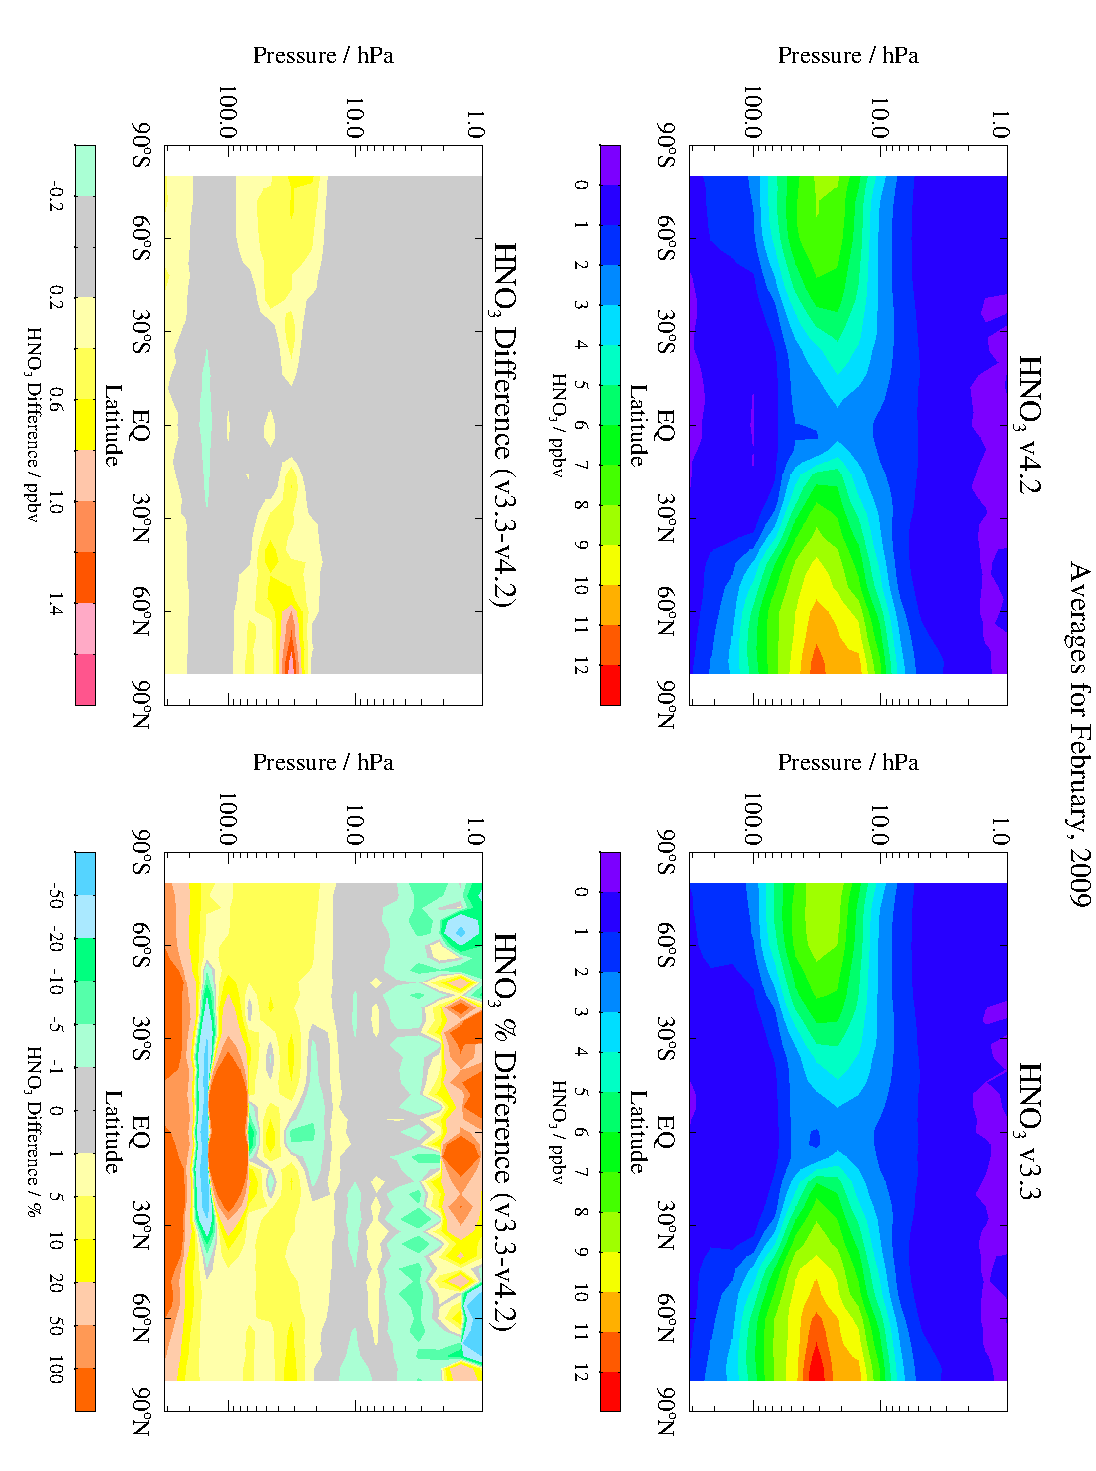
\includegraphics[angle=90,width=\linewidth]{figures/InspectZMContour_HNO3--v4-2_HNO3--v3-3_2009m02_LatPress-All}
\caption{V3.3 (top left) and v4.1 (top right) zonal mean HNO\cs3 for
 February~2009, and differences (v3.3\,$-$\,v4.1) expressed in ppbv
 (bottom left) and percent (bottom right).  Each version is screened with
  the recommended criteria.}
\label{fig:zmv3v4diffs}
\end{figure}


\subsection*{Resolution}
\onestandardavk{HNO3}{HNO\cs3}%

The resolution of the retrieved data can be described using ``averaging
kernels'' \citep[e.g.,][]{Rodgers00}; the two-dimensional nature of the
MLS data processing system means that the kernels describe both vertical
and horizontal resolution.  Smoothing, imposed on the retrieval system
in both the vertical and horizontal directions to enhance retrieval
stability and precision, reduces the inherent resolution of the
measurements.  Consequently, the vertical resolution of the \thisv
HNO\cs3 data, as determined from the full width at half maximum of the
rows of the averaging kernel matrix shown in Figure~\ref{fig:AvkHNO3},
is 3\,--\,4\,km through most of the useful range, degrading to
\texttildelow4.5\,km at 22\,hPa and some levels in the upper
stratosphere (see Table~\ref{tab:HNO3Summary}).  Note that the averaging
kernels for the 215 and 316-hPa retrieval surfaces overlap over most of
their depth, indicating that the 316-hPa retrieval provides little
independent information.  Figure~\ref{fig:AvkHNO3} also shows horizontal
averaging kernels, from which the along-track horizontal resolution is
determined to be 400\,--\,500\,km over most of the vertical range,
improving to 250\,--\,300\,km between 15 and 4.6\,hPa, and degrading to
600\,--\,700\,km at 1.5 and 1\,hPa.  The cross-track resolution, set by
the widths of the fields of view of the \mbox{190-GHz} and
\mbox{240-GHz} radiometers, is \texttildelow10\,km.  The along-track
separation between adjacent retrieved profiles is 1.5\degsym\ great
circle angle (\texttildelow165\,km), whereas the longitudinal separation
of MLS measurements, set by the Aura orbit, is 10\degsym\,--\,20\degsym\
over low and middle latitudes, with much finer sampling in the polar
regions.

\subsection*{Precision}

\begin{figure}
\centering\includegraphics[width=8.4cm]{figures/ComparePrecision2Panel_HNO3_NQC}
\caption{Precision of the (left) v3.3 and (right) v2.2 MLS HNO\cs3
  measurements for four representative days (see legend).  Solid lines
  depict the observed scatter in a narrow equatorial band (see text);
  dotted lines depict the theoretical precision estimated by the
  retrieval algorithm.\label{fig:PrecProf}}
\end{figure}

The precision of the MLS HNO\cs3 measurements is estimated empirically
by computing the standard deviation of the profiles in the
20\degsym-wide latitude band centered around the equator, where natural
atmospheric variability should be small relative to the measurement
noise.  Because meteorological variation is never completely negligible,
however, this procedure produces a upper limit on the precision-related
variability.  As shown in Figure~\ref{fig:PrecProf}, the observed
scatter in the \thisv data is \texttildelow0.5\,--\,0.6\,ppbv throughout
the range from 215 to 3.2\,hPa, and increases sharply at lower
pressures.  The scatter is essentially invariant with time, as seen by
comparing the results for the different days shown in
Figure~\ref{fig:PrecProf}.  An alternative method using the difference
between ascending and descending values at orbit crossings yields very
similar estimates.

The single-profile precision estimates cited here are, to first order,
independent of latitude and season, but it should be borne in mind that
the large geographic variations in HNO\cs3 abundances gives rise to a
wide range of signal to noise ratios.  At some latitudes and altitudes
and in some seasons, HNO\cs3 abundances are smaller than the
single-profile precision, necessitating the use of averages for
scientific studies.  In most cases, precision can be improved by
averaging, with the precision of an average of $N$ profiles being
1/$\sqrt{N}$ times the precision of an individual profile (note that
this is not the case for averages of successive along-track profiles,
which are not completely independent because of horizontal smearing).

The observational determination of the precision is compared in
Figure~\ref{fig:PrecProf} to the theoretical precision values reported
by the Level~2 data processing algorithms.  Although the two estimates
compare very well between 215 and 15\,hPa, at pressures smaller than
10\,hPa the predicted precision substantially exceeds the observed
scatter.  This indicates that the a priori information and the vertical
smoothing applied to stabilize the retrieval are influencing the results
at the higher retrieval levels.  Because the theoretical precisions take
into account occasional variations in instrument performance, the best
estimate of the precision of an individual data point is the value
quoted for that point in the L2GP files, but it should be borne in mind
that this approach overestimates the actual measurement noise at
pressures less than 10\,hPa.  Conversely, the observed scatter at
pressures higher than 100\,hPa is somewhat larger than the theoretical
precision in \thisv and much larger than the theoretical precision in
v3.3.  This is related to the spikes and increased noise in the UTLS in
v3.3, and can be seen to be much improved in \thisv.  Nevertheless, some
outliers in this region persist in \thisv.  Procedures for screening
outliers in the UTLS are discussed below.

\subsection*{Accuracy}

The effects of various sources of systematic uncertainty (e.g.,
instrumental issues, spectroscopic uncertainty, and approximations in
the retrieval formulation and implementation) on the MLS v3.3 HNO\cs3
measurements were quantified through a comprehensive set of retrieval
simulations; results for \thisv, to be completed at a later date, are
expected to be similar.  The results of the v3.3 uncertainty analysis
are summarized in Table~\ref{tab:HNO3Summary}; see
\citet{SanteeEtal07hno3} for further details of how the analysis was
conducted and the magnitude of the expected biases, additional scatter,
and possible scaling errors each source of uncertainty may introduce
into the data.  In aggregate, systematic uncertainties are estimated to
induce in the HNO\cs3 measurements biases that vary with altitude
between $\pm$0.5 and $\pm$2\,ppbv and multiplicative errors of
$\pm$5\,--\,15\% through most of the stratosphere, rising to
\mbox{\texttildelow$\pm$30\%} at 215\,hPa and \texttildelow50\% at and
above 2.2\,hPa.  These uncertainty estimates are generally consistent
with the results of comparisons with correlative datasets, as discussed
briefly below.

\subsection*{Data screening -- all data}
\label{sec:HNO3Screening}

\begin{description}
\item[Pressure range:] \screeningrule{215\,--\,1.5\,hPa}
  \standardrangestatement
\standardprecisionrule
\evenstatusrule
\end{description}
\subsection*{Data screening -- upper troposphere, lower stratosphere
  (pressures of 22\,hPa or greater)}

The \texttt{Quality} and \texttt{Convergence} fields included in the
\texttt{HNO3} swath in the standard \texttt{L2GP-HNO3} files are
appropriate for use in screening at levels at and below (that is,
pressures greater than) 22\,hPa.  For those levels:

\begin{description}
\item[Quality:] \qualityrule{0.8}

  This threshold for \texttt{Quality} typically excludes
  \texttildelow1\,--\,3\% of HNO\cs3 profiles on a daily basis; it is a
  conservative value that potentially discards a significant fraction of
  ``good'' data points while not necessarily identifying all ``bad''
  ones.  A significant fraction of the HNO\cs3 profiles in \thisv show a
  ``notch'', with unexpectedly low values at 100\,hPa and high values at
  147\,hPa; many such profiles are removed by using this
  \texttt{Quality} threshold.

\item[Convergence:] \convergencerule{1.03}

  On a typical day this threshold for \texttt{Convergence} discards a
  very small fraction of the data, rarely eliminating more than
  0.1\% of the HNO\cs3 profiles.  Some such profiles show unphysical
  behavior.

\item[Clouds:] \screeningrule{Clouds impact HNO\cs3 data in the UTLS,
    see discussion below and the discussion on ``outliers'' that follows.}

  Nonzero but even values of \texttt{Status} indicate that the profile
  has been marked as questionable, typically because the measurements
  may have been affected by the presence of thick clouds.  Globally
  \texttildelow1\,--\,2\% of profiles are identified in this manner,
  with the fraction of profiles possibly impacted by clouds rising to
  \texttildelow5\% on average in the tropics.  Clouds
  generally have little influence on the stratospheric HNO\cs3 data.  In
  the lowermost stratosphere and upper troposphere, however, thick
  clouds can lead to spikes in the HNO\cs3 mixing ratios in the
  equatorial regions.

  Therefore, it is recommended that at and below 68\,hPa, in addition to
  performing the ``outlier screening'' described below, all profiles
  with nonzero values of Status be discarded because of the potential
  for cloud contamination.  While this will reject some profiles that
  are probably not significantly impacted by cloud effects, and the
  number of profiles rejected that are not flagged by other criteria is
  small (\texttildelow0.5 to 1\% of total profiles), it does eliminate
  some unphysical profiles that are not flagged by the outlier
  screening.

\item[Outliers:] \screeningrule{Alternative screening approaches in the
    UTLS remove outliers while reducing ``false positives''}

  While the number, and particularly the extreme values of, outliers in
  \thisv HNO\cs3 at levels between 316 and 100 (sometimes to 68) hPa is
  greatly reduced over that in v3.3, such outliers are still present.
  These typically appear as highly negative mixing ratios at the lowest
  several retrieval levels, often as part of oscillatory profiles with
  unrealistically high values at higher altitudes.  A simple procedure
  is recommended to screen such profiles based on eliminating all
  profiles with large negative mixing ratios at pressure levels between
  316 and 68\,hPa.  Through extensive examination of data screened in
  this way, flagging profiles that have either HNO\cs3 vmr less than
  $-2.0$\,ppbv at 316\,hPa or less than $-1.6$\,ppbv at any level
  between 215 and 68\,hPa eliminates most of the troublesome outliers,
  including those with positive vmr spikes overlying the negative ones
  that are directly flagged by these criteria.  This screening procedure
  is recommended for any studies focusing on the UTLS\@. A detailed
  description of the testing procedure for this screening is given by
  \citet{EOSMLSV33V34Quality}, and this testing has demonstrated that it
  effectively removes most of the suspect profiles that are not
  eliminated by requiring Status to be zero.

  Figure~\ref{fig:outlierprofs} shows an example of the results of
  screening profiles by each of the \texttt{Quality},
  \texttt{Conver\-gence} and the recommended outlier flagging on a
  typical `bad' day (i.e., one with a relatively large number of
  outliers) in \thisv versus v3.3.  The \texttt{Quality} screening
  removes many of the profiles that are strongly negative at the bottom,
  as well as many with the ``notch'' structure begtween 147 and
  100\,hPa.  Most or all of the remainder of the profiles that are
  strongly negative at the bottom are flagged by the outlier screening;
  many of these profiles are oscillatory, so this screening also removes
  most or all of the strong positive outliers (typically at 147\,hPa).
  Most of the profiles flagged by any of the criteria are in the
  tropics, as expected; low HNO\cs3 values in Antarctic winter resulting
  from denitrification are rarely, if ever, affected by this outlier
  screening. It is clear from this example that the outliers in \thisv
  are less frequent and much less extreme than those in v3.3
 
\end{description}

\subsection*{Data screening -- upper stratosphere (pressures of 15\,hPa
  or less)}

The above screening criteria \emph{should not be used} for 15\,hPa and
higher altitudes, as they result in filtering profiles for which all
quality indicators are good when the \texttt{Quality} and
\texttt{Convergence} values are properly taken from the 190-GHz HNO\cs3
information, and not filtering ones with indications of poor quality.
The \texttt{HNO3-190} swath has been included in the standard HNO\cs3
files for \thisv, and the appropriate \texttt{Quality} and
\texttt{Convergence} values for the 190-GHz HNO\cs3 from that swath must
be used to apply the following screening criteria:
 
\begin{description}
\item[Clouds:] \screeningrule{Profiles where the \texttt{Status} field
    for \texttt{HNO3-190} has a non-zero even number can be used without
    restriction.} Clouds generally have little influence on the
  stratospheric HNO\cs3 data at these altitudes.

\item[Quality:] \screeningrule{Only profiles with a value of the
    \texttt{Quality} field for \texttt{HNO3-190} (see
    section~\ref{sec:StatusQuality}) \emph{greater} than 0.8 should be
    used in scientific study.}

  This threshold for \texttt{Quality} typically excludes
  \texttildelow1\,--\,3\% 
  of HNO\cs3 profiles on a daily basis; it is a conservative value that
  potentially discards some ``good'' data points while not necessarily
  identifying all ``bad'' ones.  

\item[Convergence:] \screeningrule{Only profiles with a value of the
    \texttt{Convergence} field (see section~\ref{sec:StatusQuality}) for
    the \texttt{HNO3-190} product \emph{less} than 1.4 should be used in
    investigations.}

  On a typical day this threshold for \texttt{Convergence} discards
  \texttildelow0.5\,--\,1.5\% of the HNO\cs3 profiles.  Many of the
  profiles thus flagged show some unphysical behavior, especially at the
  highest altitudes in the recommended range.

\item[Outliers:] For levels at and above (pressures less than) 4.6\,hPa,
  especially at 2.2\,hPa and above, some profiles show vertically
  oscillatory behavior in conditions where HNO\cs3 is very low.  The
  \texttt{Quality} and \texttt{Convergence} criteria defined above 
  eliminate many of these profiles.
\end{description}

\begin{figure}
\begin{tabular}{@{}l@{}l@{}}
\includegraphics[width=0.5\linewidth]{figures/ProfQual0-80_Conv1-03_Fly_HNO3_2009d051_-90to90_v04-__stat0}&
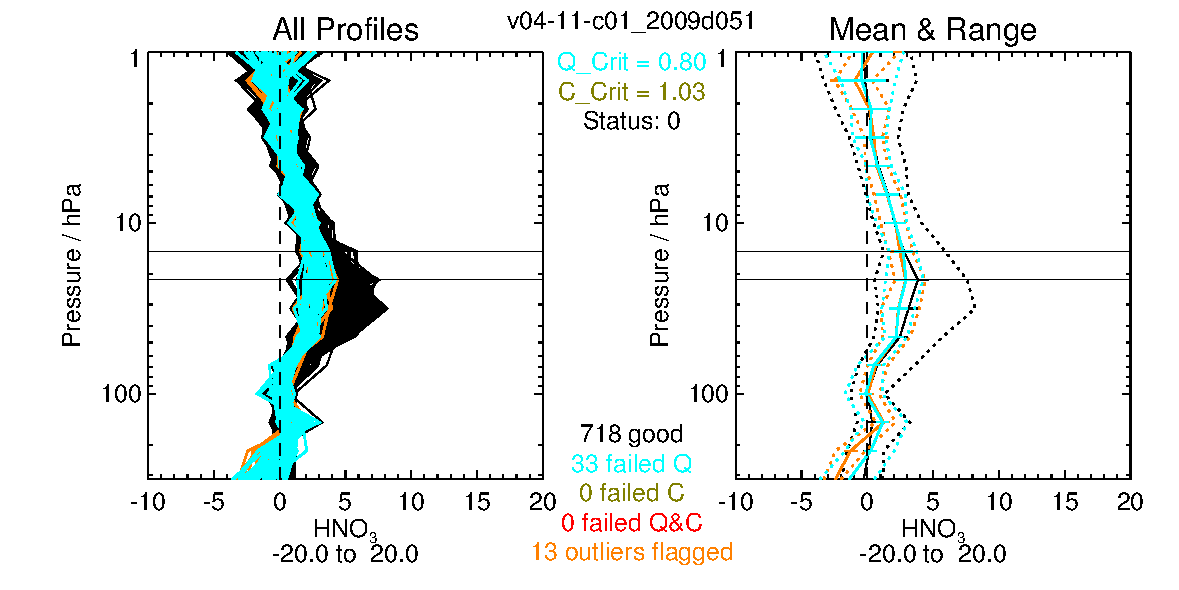
\includegraphics[width=0.5\linewidth]{figures/ProfQual0-80_Conv1-03_Fly_HNO3_2009d051_-20to20_v04-__stat0}\\
\includegraphics[width=0.5\linewidth]{figures/ProfQual0-50_Conv1-40_Fly_HNO3_2009d051_-90to90_v03-__stat0}&
\includegraphics[width=0.5\linewidth]{figures/ProfQual0-50_Conv1-40_Fly_HNO3_2009d051_-20to20_v03-__stat0}
\end{tabular}
\caption{HNO\cs3 profiles on 20~Feb~2009 color-coded by screening.  Cyan
  profiles have \texttt{Quality} less than 0.8 (0.5), olive-green
  \texttt{Convergence} greater than 1.03 (1.4), and red both
  \texttt{Quality} less than 0.8 (0.5) and \texttt{Convergence} greater
  than 1.03 (1.4) for \thisv (v3.3).  Orange profiles are those flagged
  by the simple screening procedure described above (using large
  negative mixing ratios at high pressures) after the profiles that
  failed \texttt{Quality} and/or \texttt{Convergence} tests were
  removed.  Black profiles are all those remaining (the ``good''
  profiles) after all screening.  The left panels show all individual
  profiles in the day; the right panels show the means in each category,
  with the standard deviation shown as bars and the range as dotted
  lines.  The horizontal line is at 22\,hPa, above which HNO\cs3 is from
  the 190-GHz radiometer and thus not appropriately screened by these
  criteria.  The four pairs of panels show all \thisv profiles (top
  left), \thisv profiles between $-20\degsym$ and 20\degsym\ latitude
  (top right), all v3.3 profiles (bottom left) and v3.3 profiles between
  $-20\degsym$ and 20\degsym\ latitude.}
\label{fig:outlierprofs}
\end{figure}

\subsection*{Comparisons with other datasets}

\thisv HNO\cs3 profiles generally show only small differences in
magnitude from v3.3 when each data version is screened according to the
criteria above.  Therefore, the comparisons with correlative data are
expected to be very similar to those described for v3.3 by
\citet{EOSMLSV33V34Quality}.

\begin{DIFnomarkup}
\begin{table}
\caption{Summary of Aura MLS \thisv HNO\cs3 Characteristics}\vspace{0.5ex}
\label{tab:HNO3Summary}
\begin{minipage}{\linewidth}\small
  \renewcommand{\thefootnote}{\thempfootnote}
  \centering\begin{tabular}{cccccl} \toprule
\parbox[m]{16mm}{\bfseries\centering{Pressure\\ / hPa}} &
\parbox[m]{22mm}{\bfseries\centering{Resolution\\ \mbox{V $\times$ H}%
\footnote{Horizontal resolution in along-track direction.} \\ / km}} &
\parbox[m]{16mm}{\bfseries\centering{Precision%
\footnote{Precision on individual profiles, determined from observed
 scatter in the data in a region of minimal atmospheric variability.} \\/ ppbv}} &
\parbox[m]{18mm}{\bfseries\centering{Bias\\uncertainty%
\footnote{Values should be interpreted as \mbox{2-$\sigma$} estimates
 of the probable magnitude.}\\ / ppbv}} &
\parbox[m]{18mm}{\bfseries\centering{Scaling\\uncertainty%
\footnotemark[\value{mpfootnote}]\\/ \%}} &
\textbf{Comments} \\
%
\midrule
%
0.68\,--\,0.001 & ---  & ---    & ---    & --- & Unsuitable for scientific
  use\\
%
1.0 & 4 $\times$ 650\,--\,750  & $\pm$1.2 & $\pm$0.5 & $\pm$50\% & Caution, averaging
recommended \\
%
1.5 & 4.5 $\times$ 550\,--\,600 & $\pm$1.2  & $\pm$0.5 & $\pm$50\% & Averaging recommended \\
%
2.1 & 5 $\times$ 450\,--\,500 & $\pm$0.8  & $\pm$1.0 & $\pm$50\% & \\
%
3.2 & 4.5 $\times$ 400 & $\pm$0.6  & $\pm$0.6  & $\pm$10\,--\,15\% & \\
%
4.6 & 4 $\times$ 300\,--\,350 & $\pm$0.6  & $\pm$0.6  & $\pm$10\,--\,15\% & \\
% 
15\,--\,6.8  & 3\,--\,4 $\times$ 250\,--\,300 & $\pm$0.6 & $\pm$1\,--\,2  &
  $\pm$10\% & \\
%
22 & 4.5 $\times$ 500 & $\pm$0.6 & $\pm$1\,--\,2 &
$\pm$10\% & \\
%
147\,--\,32  & 3\,--\,4 $\times$ 350\,--\,400 & $\pm$0.6 & $\pm$0.5\,--\,1 &
$\pm$5\,--\,10\% & \\
%
215        & 4\,--\,4.5 $\times$ 450  & $\pm$0.6 & $\pm$1    &
\texttildelow$\pm$30\% & \\
%
316        & ---      & ---    & ---    & --- & Unsuitable for
scientific use\\
%
1000\,--\,464  & ---      & ---    & ---    & --- & Not retrieved\\
%
\bottomrule
\end{tabular}\par
\end{minipage}
\end{table}
\end{DIFnomarkup}

%%% Local Variables: 
%%% mode: latex
%%% TeX-master: "v4-x-report"
%%% End: 

 \speciestitle{Peroxy Radical}{HO\cs2}{HO2}{%
\item[Useful range:] 22\,--\,0.046\,hPa
\item[Contact:] Shuhui Wang, \email{Shuhui.Wang@jpl.nasa.gov}}

\subsection*{Introduction}

A description of HO\cs2 data quality, precision, systematic errors, and
validation for an earlier version, v2.2, is given in
\citet{PickettEtal08}. An early validation using v1.5 software is also
described in \citet{PickettEtal06}. While there are significant
improvements from v1.5 to \prevv, the HO\cs2 data quality in \thisv is
generally similar to \prevv.  The estimated uncertainties, precisions,
and resolution for \thisv HO\cs2 are summarized below in
Table~\ref{tab:HO2Summary}. Note that the systematic uncertainties are
from \prevv and, while they are not expected to change significantly in
\thisv, they will be updated for this new version at a later date.

An algorithm to retrieve daily zonal means of HO\cs2 over an extended
vertical range by first averaging the radiances has been developed by
the MLS team \citep{MillanEtal15}. This alternative dataset is the first
long-term daytime and nighttime HO\cs2 satellite record covering the
stratosphere and the mesosphere. In the near future, this dataset will
be available at the GFSC DISC, in the meantime, those interested in
using it are advised to contact the MLS team.

\subsection*{Resolution}

Figure~\ref{fig:AvkHO2} shows the HO\cs2 averaging kernel for daytime at
70\degsym N and the Equator. The latitudinal variation in the averaging
kernel is very small. The vertical resolution for pressures greater than
0.1\,hPa is generally about 5\,km.

\subsection*{Precision}

A typical HO\cs2 profile and the associated precisions (for both \prevv
and \thisv) are shown in Figure~\ref{fig:HO2profiles}. The profile is
shown in both volume mixing ratio (vmr) and density units. All MLS data
are reported in vmr for consistency with the other retrieved molecules.
However, use of density units (10\cp{6}\,cm\cp{$-$3}) reduces the
apparent steep gradient of HO\cs2 vertical profile, allowing one to see
the profile with more detail. The night HO\cs2 profile is expected to
exhibit a narrow layer near the altitudes of the nighttime OH layer at
\texttildelow82\,km \citep{PickettEtal06niteOH}, which is not shown in
Figure~\ref{fig:HO2profiles} since MLS HO\cs2 data is not recommended
for altitudes above 0.046\,hPa (\texttildelow70\,km). Precisions are
such that an HO\cs2 zonal average within a 10\degsym\ latitude bin can
be determined with better than 10\% relative precision with 20 days of
data (\texttildelow2000 samples) for most pressure levels over
22\,--\,0.046\,hPa.

\oneverticalavk{HO2}{HO\cs2}%

\begin{figure}
\begin{tabular}{@{}l@{}l@{}}
\includegraphics[width=0.5\linewidth]{figures/plot-HO2v4-a}&
\includegraphics[width=0.5\linewidth]{figures/plot-HO2v4-b}\\
\includegraphics[width=0.5\linewidth]{figures/plot-HO2v4-c}&
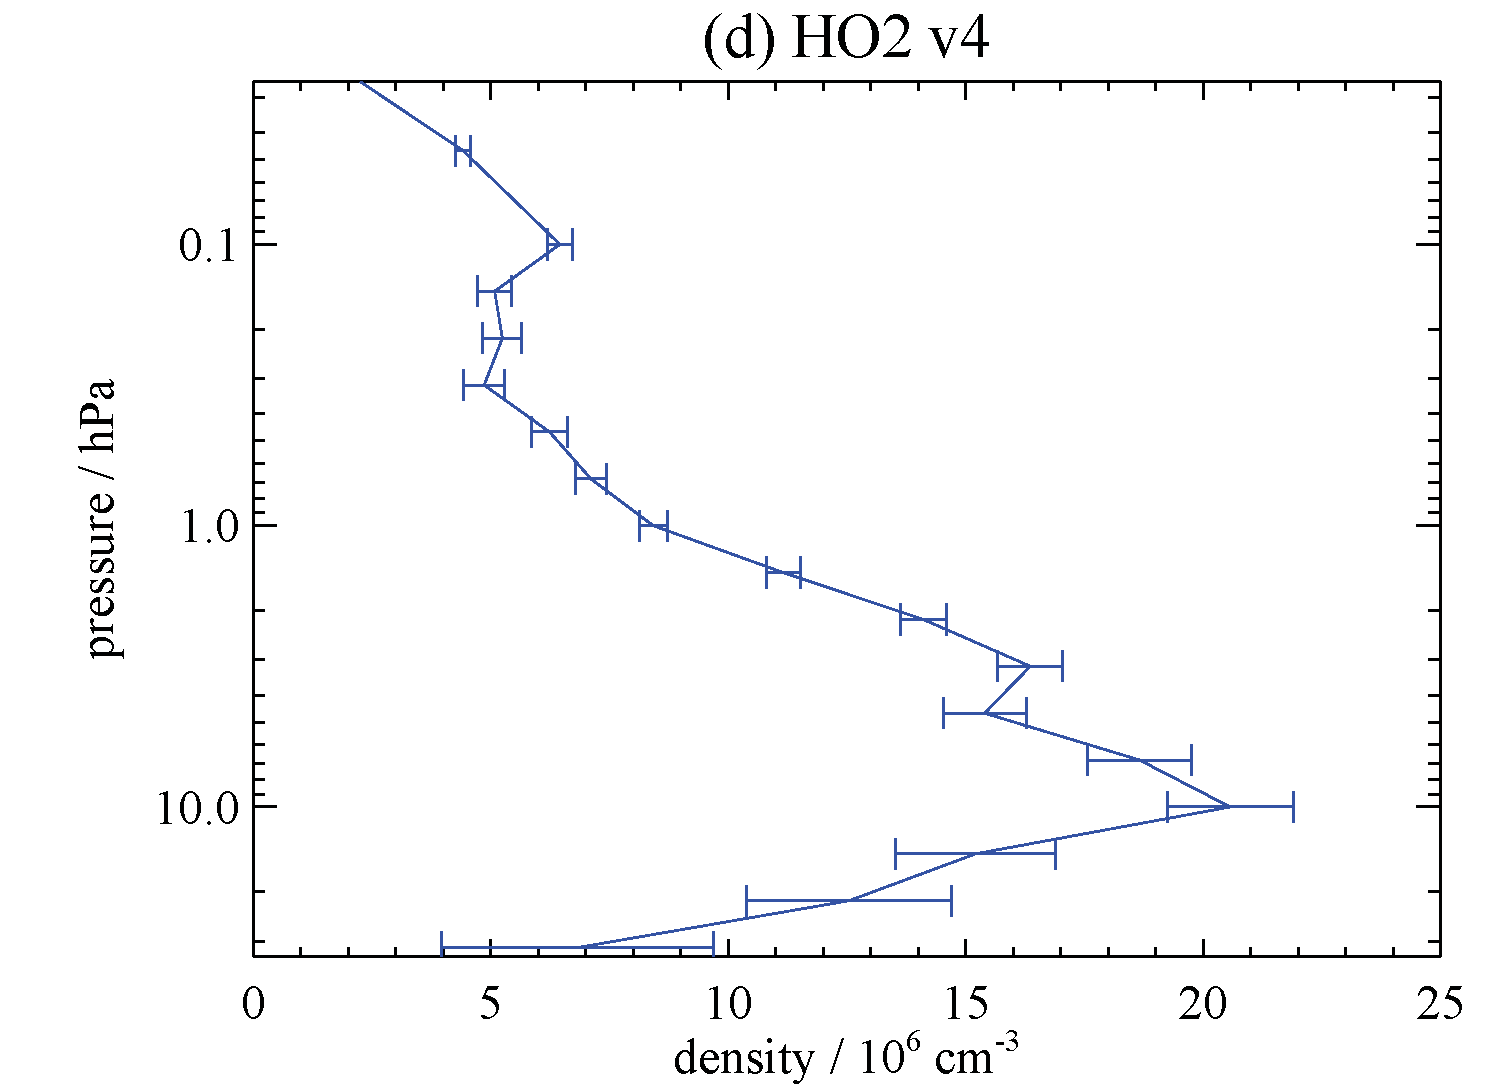
\includegraphics[width=0.5\linewidth]{figures/plot-HO2v4-d}\\
\includegraphics[width=0.5\linewidth]{figures/plot-HO2v3-e}&
\includegraphics[width=0.5\linewidth]{figures/plot-HO2v3-f}%
\end{tabular}
\caption{Monthly zonal mean of retrieved HO\cs2 and its estimated
  precision (horizontal error bars) for September, 2005 averaged over
  29\degsym N to 39\degsym N. Panel (a) shows \thisv HO\cs2 vmr vs.\
  pressure for day (black) and night (blue). Panel (b) shows the same
  data plotted for the stratosphere as a day-night difference (note that
  a day-night difference is required for HO\cs2 for all pressure
  levels). Panel (c) shows the same data in (a) converted into density
  units. Panel (d) shows the day-night differences for the data in panel
  (c). Panels (e) and (f) are equivalent to (c) and (d) but using v2.2
  data. The average in panels (a)\,--\,(d) using \thisv data includes 3052
  profiles, while the average in panels (e)\,--\,(f) using v2.2 data
  includes 2695 profiles.}
\label{fig:HO2profiles}
\end{figure}

\subsection*{Accuracy}

Table~\ref{tab:HO2Summary} summarizes the accuracy expected for HO\cs2.
The scaling uncertainty is the part of the systematic uncertainty that
scales with HO\cs2 concentration, e.g. spectroscopic line strength. Bias
uncertainty is the part of the uncertainty that is independent of
concentration. For both bias and scaling uncertainty, quantification of
the combined effect in MLS calibration, spectroscopy etc., on the data
product was determined by calculating the effects of each source of
uncertainty. These accuracy calculations are for \prevv products. While
no significant change is expected from \prevv to \thisv, a comprehensive
error analysis for \thisv will be conducted. Bias uncertainty can be
eliminated by taking day-night differences over the entire recommended
pressure range. The accuracy of the HO\cs2 measurement due to systematic
errors is a product of scaling uncertainty and the observed HO\cs2
concentration. The overall uncertainty is the square root of the sum of
squares of the precision and accuracy.

\subsection*{Data screening}
\label{sec:HO2Screening}

It is recommended that HO\cs2 data values be used in scientific
investigations if all the following tests are successful:
\begin{description}
\item[Pressure range:] \screeningrule{22\,--\,0.046\,hPa}
  \standardrangestatement \standardprecisionrule \evenstatusrule
\item[Quality:] \screeningrule{MLS \thisv HO\cs2 data can be used
    irrespective of the value of the \texttt{Quality} field.}
\item[Convergence:] \convergencerule{1.1} In version v2.2 this
  test often fails for 100 out of 3500 profiles in a day. In the current
  version, \thisv, there are often zero or very few non-convergence
  profiles.
\end{description}

\subsection*{Artifacts}
Currently there are no known artifacts in the HO\cs2 product. The
primary limitation is the precision and the altitude range.

\subsection*{Review of comparisons with other datasets}
HO\cs2 data from MLS v2.2 software have been validated with two
balloon-borne remote-sensing instruments. Details of the comparison are
given in \citet{PickettEtal08}. Differences between v2.2 and \thisv show
no differences large enough to alter results of previous validation
studies.

\begin{table}
  \caption{Summary of precisions, resolution, and uncertainties for
    the MLS \thisv HO\cs2 product}
\vspace{\tablecaptionsep}
\label{tab:HO2Summary}
\begin{minipage}{\linewidth}
\small\centering\begin{tabular}{rccccl}
\toprule
\parbox{10ex}{\bfseries\centering Pressure\\ /\,hPa} &
\parbox{10ex}{\bfseries\centering Vertical\\ resolution\\ \,km} &
\parbox{10ex}{\bfseries\centering Precision\footnote{Precision for a
    single profile} / \mbox{10\cp6 cm\cp{$-$3}}} &
\parbox{15ex}{\bfseries\centering Bias uncertainty / \mbox{10\cp6 cm\cp{$-$3}}} &
\parbox{12ex}{\bfseries\centering Scaling uncertainty / \%} &
\textbf{Comments} \\
\midrule
 $<$ 0.03\,hPa  & ---   & ---               & --- & --- & Unsuitable for scientific use\\
 0.046\,hPa     & 10    & 6                 & 0.39& 22  & Use day--night difference \\
 0.10\,hPa      & 7     & 10                & 0.46& 16  & Use day--night difference \\
 1.0 \,hPa      & 5     & 11                & 1.1 & 6   & Use day--night difference \\
 10  \,hPa      & 4     & 50                & 37  & 20  & Use day--night difference \\
 $>$ 22\,hPa    & ---   & ---               & --- & --- & Unsuitable for scientific use\\
\bottomrule
\end{tabular}
\end{minipage}
\end{table}

%%% Local Variables:
%%% mode: latex
%%% TeX-master: "v4-x-report"
%%% End:
 \speciestitle{Hypochlorous Acid}{HOCl}{HOCl}{%
\item[Useful range:] 10\,--\,2.2\,hPa 
\item[Contact:] Lucien Froidevaux, \email{Lucien.Froidevaux@jpl.nasa.gov}}

\subsection*{Introduction}

There has been little change in the v4.2 HOCl retrieval results, in
comparison to v3.3/v3.4. We provide below sample mean HOCl distributions
for the two data versions, and their differences. Otherwise, previous
information regarding this species remains largely unchanged; the main
points are mentioned here mainly for new data users.


The HOCl retrieval is quite noisy for individual profiles and HOCl data
require some averaging (e.g., in 10\degsym\ zonal means for one or more
weeks) to get useful precision of better than 10\,pptv, in comparison to
typical upper stratospheric HOCl abundances of 100\,--\,150\,pptv.
Table~\ref{tab:HOClSummary} summarizes the MLS HOCl resolution,
precision, and accuracy estimates for the upper stratosphere.  More
discussion and a brief validation summary are given in the following
sections, along with data screening recommendations, which should be of
particular interest to MLS data users.

\subsection*{Changes from v3.3/v3.4}
There were no algorithmic changes relating to HOCl for the v4.2
retrievals.  Small differences in HOCl abundances (see below) are likely
related mainly to small changes in tangent pressure and/or temperature.

The background observed in the 640-GHz radiances includes emissions from
N\cs2, O\cs2, and H\cs2O.  There are laboratory-based and ground-based
models for the continuum absorptions that are the basis for the MLS
absorption model \citep[][and references therein]{PardoEtal01}.  These
models were tested against MLS extinction measurements from the wing
channels in the 640-GHz radiometer.  The latitude dependence of this
extinction was found to agree better with the expected most plus dry
continuum extinction values if the dry and moist continuum functions
were scaled by factors close to 20$\%$; however, this is not a change
from the v3.3/v3.4 retrievals.

A comparison plot showing zonal average upper stratospheric HOCl
contours (from 10 to 2\, hPa) and differences between the two data
versions for a typical month (March, 2009) is provided in Figure
~\ref{fig:MLSv3v4HOClContour}.  The v4.2 HOCl abundances are mostly
slightly larger than the v3.3 retrievals, typically by only a few pptv
(a few percent).  The estimated precision values are essentially
unchanged from v3.3.

\begin{figure}
  \centering\includegraphics[angle=90,width=1.\linewidth]{figures/Fig-HOCl-ZMContours-v3-3-v4-2_2009m03}
  \caption{Zonal averages for upper stratospheric MLS HOCl profiles
    during March, 2009, showing the MLS v3.3 HOCl mixing ratio contours
    (top left panel), the v4.2 contours (top right panel), and their
    differences in pptv (v4.2 minus v3.3, bottom left panel) and percent
    (v4.2 minus v3.3 versus v3.3, bottom right panel). }
\label{fig:MLSv3v4HOClContour}
\end{figure}

\subsection*{Resolution}
\oneverticalavk{HOCl}{HOCl}%

Based on the width of the averaging kernels shown in
Figure~\ref{fig:AvkHOCl}, the vertical resolution for upper
stratospheric HOCl is $\sim$6\,km (significantly worse than the 640-GHz
radiometer vertical field of view width of 1.4\,km).  This reflects the
choice of smoothing constraints for HOCl which favor precision over
vertical resolution.

\subsection*{Precision}

The estimated single-profile precision reported by the Level~2 software
is about 300 to 400\,pptv in the upper stratosphere.  A more useful
number of 10\,pptv is quoted in Table~\ref{tab:HOClSummary} for the
typical precision of a 10\degsym\ weekly zonal means for this product.

\subsection*{Accuracy}

The accuracy estimates shown in Table~\ref{tab:HOClSummary} come from a
formal quantification of the combined effects of possible systematic
errors in MLS calibration, spectroscopy, etc.\ on the HOCl retrievals
\citep{ReadEtal07}.  These values are intended to represent $2\sigma$
estimates of accuracy.  The largest contributors to possible errors for
HOCl are contaminant species, gain compression, and sideband ratio
uncertainties.  The Table gives a range of error estimates (for low and
high pressures).  The average changes for upper stratospheric HOCl
between v3.3 and v4.2 are well within the quoted accuracy estimates
(which may be somewhat conservative).

\subsection*{Data screening}
\label{sec:HOClScreening}
\begin{description}
\item[Pressure range:] \screeningrule{10\,--\,2.2\,hPa}
  \standardrangestatement\ Artifacts (negative averages) for pressures
  larger than about 10\,hPa currently make this product unsuitable for
  use in the lower stratosphere. Regarding the topmost altitude range,
  the sensitivity to \emph{a priori} increases rapidly at pressures of
  1\,hPa or less; we continue to recommend the use of (average) HOCl
  values only up to 2.2\, hPa.  \standardprecisionrule \evenstatusrule

\item[Quality field:] \screeningrule{Only profiles with a value of the
    \texttt{Quality} field \emph{greater} than 1.2 should be used.}

  This criterion removes profiles with the poorest radiance fits,
  typically less than 0.1$\%$ of the daily profiles. For HOCl (and for
  other 640-GHz MLS products), this screening correlates well with the
  poorly converged sets of profiles (see below); we recommend the use of
  both the \texttt{Quality} and \texttt{Convergence} fields for data
  screening.

\item[Convergence field:] \screeningrule{Only profiles with a value of
    the \texttt{Convergence} field \emph{less} than 1.05 should be
    used.} For the vast majority of profiles (99$\%$ or more for most
  days), this field is less than 1.05.  Nevertheless, on occasion, sets
  of profiles (typically one or more groups of ten profiles, retrieved
  as a `chunk') have this \texttt{Convergence} field set to larger
  values, and should be discarded.

\item[Clouds:] \cloudsokrule

\end{description}

\subsection*{Review of comparisons with other datasets}

The MLS HOCl retrievals exhibit the expected morphology in monthly mean
latitude / pressure contour plots; for example, such plots for September
months from MLS compare favorably, to first-order, with results produced
by the Michelson Interferometer for Passive Atmospheric Sounding (MIPAS)
for September, 2002 \citep{VonClarmannEtal06}.  MLS HOCl averages at
midlatitudes are close to the results from balloon-borne infrared
measurements. Generally favorable comparisons (within the error bars)
have been made of the diurnal changes in upper stratospheric HOCl
between Aura MLS (v3.3), other satellite datasets, and a 1-D
photochemical model \citep{KhosraviEtal13}.

\subsection*{Artifacts}
\begin{itemize} 
\item The 640-GHz radiometer bands 10 (for ClO) and 29 (for HOCl) were
  turned off for a few time periods in 2006 to investigate degradation
  issues that might affect these channels in the future.  These bands
  were off on April 8,9, and 10, 2006, and also for April 17, 2006
  (after 19:52 UT) through May 17, 2006.  There are essentially no
  useful HOCl (or ClO) data for these time periods.  The v4.2 (as for
  the v3.3/v3.4) software correctly flags these incidents with poor
  (odd) \texttt{Status} values (which should be screened out).
\item There are still significant artifacts in the mean values (large
  negative values) for HOCl in the lower stratosphere, where the use of
  this product is not recommended.
\item Users should screen out the non-converged and poorest quality HOCl
  profiles, as such profiles (typically a very small number per day)
  tend to behave unlike the majority of the other MLS retrievals.  See
  the criteria listed above.
\end{itemize}  

\begin{table}
\caption{Summary for MLS hypochlorous acid}\vspace{0.5ex}
\label{tab:HOClSummary}
\begin{minipage}{\linewidth}\small
\centering\begin{tabular}{ccccccl}
\toprule
\parbox[m]{15mm}{\centering\textbf{Pressure}} &
\multicolumn{2}{c}{\parbox[m]{15mm}{\centering\textbf{Precision\footnote{Precision ($1\sigma$) 
for 1 week/10 degrees zonal means or 2 weeks/5 degrees zonal means}}}} &
\parbox[m]{24mm}{\centering\textbf{Vertical\\ Resolution\\km}} &
\multicolumn{2}{c}{\parbox[m]{15mm}{\centering\textbf{Accuracy\footnote{$2\sigma$ estimate from systematic 
uncertainty characterization tests}\\}}} 
&
\textbf{Comments} \\
\textbf{hPa} & \textbf{pptv} & \textbf{\%} & \textbf{km}& \textbf{pptv} & \textbf{\%} & \\
\midrule
1.5 or less & --- & ---   & ---  & --- & ---  & Unsuitable for scientific use \\ 
2.2 to 10   &  10 & 10    &   6  & 30\,--\,80 & \texttildelow30\,--\,100 \\ 
15 or more  & --- & ---   & ---  & --- &  --- & Unsuitable for scientific use \\    
\bottomrule
\end{tabular}
\end{minipage}
\end{table}

%%% Local Variables: 
%%% mode: latex
%%% TeX-master: "v4-x-report"
%%% End: 
 \speciestitle{Cloud Ice Water Content}{IWC}{IWC}{%
\item[Units:] g/m\cp3
\item[Useful range:] 215\,--\,83\,hPa
\item[Contact: ] Alyn Lambert, \email{Alyn.Lambert@jpl.nasa.gov}}

\subsection*{Introduction}

The MLS IWC is retrieved from cloud-induced radiances (\Tcir) of the
240-GHz window channel in a separate processing step after the
atmospheric state (Temperature and tangent pressure) and important
gaseous species (H\cs2O, O\cs3, HNO\cs3) have been finalized in the
retrieval processing.  The derived \Tcir\ are binned onto the standard
horizontal (1.5\degsym\ along track) and vertical (12 surfaces per
decade change in pressure) grids, and converted to IWC using the modeled
\Tcir\,--\,IWC relations \citep{WuEtal06}.  The standard IWC profile has
a useful vertical range between 215\,--\,83\,hPa although the validation
has been conducted for a subset of the range of IWC values. IWC
measurements beyond the value ranges specified in
Table~\ref{tab:IWCSummary} are to be regarded currently as giving only
qualitative information on cloud ice.  They require further validation
for quantitative interpretation.

\subsection*{Resolution}

In the IWC ranges specified in Table~\ref{tab:IWCSummary}, each MLS
measurement can be quantitatively interpreted as the average IWC for the
volume sampled. This volume has a vertical extent of \texttildelow3\,km, with
\texttildelow300\,km and 7\,km along and cross track respectively.

\subsection*{Precision}

The precision values quoted in the IWC files do not represent the true
precision of the data.  The precision for a particular measurement must
be evaluated on a daily basis using the method described in the
screening section below.  The precision listed in
Table~\ref{tab:IWCSummary} reflects typical values obtained from the
method described below.

\subsection*{Accuracy}

The IWC accuracy values listed in Table~\ref{tab:IWCSummary} are
estimates from comparisons of the earlier v2.2 MLS data product with
CloudSat and detailed analyses on the v2.2 error budget can be found in
\citet{WuEtal08}.

\subsection*{Data screening}
\label{sec:IWCScreening}
\begin{description}
\item[Pressure range (215\,--\,83\,hPa):] \standardrangestatement\ The
  maximum detectable IWC is \texttildelow100\,mg/m\cp3.
\item[Use Temperature Status, Quality and Convergence:] The user is
  recommended to screen the IWC data using the \texttt{Status} field in
  the collocated temperature profile to exclude bad retrievals
  \citep{SchwartzEtal08}. In other words, only IWC profiles for which
  temperature \texttt{Status} is an even number should be used.
  Similarly, the users should only use IWC profiles where the
  corresponding Temperature profiles have \emph{Quality} of 0.9 or
  larger and \texttt{Convergence} less than 1.03.
\item[Other screening:] The IWC product derives from differences between
  measured radiances and those predicted assuming cloud free conditions.
  Spectroscopic and calibration uncertainties give rise to temporally
  and geographically varying biases in this difference, and hence the
  IWC product.  These biases must be iteratively identified and removed,
  using a ``$2\sigma$\,--\,$3\sigma$'' screening method, as described
  below.

\begin{enumerate}
\item Uncertainties in spectroscopy and atmospheric composition are
  manifested as residual biases in the IWC fields which should be
  identified and removed as follows.  IWC data should be averaged in a
  10\degsym\ latitude bins and outliers rejected iteratively by
  excluding measurements greater than $2\sigma$ standard deviation about
  the mean ($\mu$) of the bin. Repeat the $\sigma$ and $\mu$
  calculations after every new set of rejections.  Convergence is
  usually reached within 5\,--\,10 iterations, and the final $\sigma$ is
  the estimated precision for the IWC measurements.
\item Interpolate the final $\sigma$ and $\mu$ to the latitude of
  each measurement, and subtract $\mu$ from IWC for each measurement.
\item Finally, apply the 3$\sigma$ threshold to determine if an IWC
  measurement is statistically significant. In other words, it must have
  $\text{IWC} > \mu + 3\sigma$ in order to be considered as a
  significant cloud hit.  The $3\sigma$ threshold is needed for cloud
  detection since a small percentage of clear-sky residual noise can
  result in a large percentage of ``false alarms'' in cloud detection.
\end{enumerate}
\end{description}

\subsection*{Artifacts}

At wintertime mid-to-high latitudes, strong stratospheric gravity waves
may induce large fluctuations in the retrieved tangent pressure, and
cause false cloud detection with the 2$\sigma$\,--\,3$\sigma$ screening
method. The false cloud detection seems to affect the 100\,hPa pressure
level most, as expected for such impact coming from the lower
stratosphere.

\subsection*{Comparisons with other datasets}

Compared to v2.2 IWC the \thisv IWC values are within 5\% over the
pressure range 215\,--\,100\,hPa and generally the random noise in
\thisv IWC is larger than in v2.2 (see Figure~\ref{fig:IWC} and
Table~\ref{tab:IWCSummary}).  Apart from the differences noted above,
the MLS \thisv IWC is similar to the MLS v2.2 product described and
validated in \citet{WuEtal08}.  A revised validation paper for IWC is
not planned in the near future and users are encouraged to read
\citet{WuEtal08} for more information.

Comparisons between v2.2 MLS and CloudSat IWC showed good agreement with
PDF differences $<$50\% for the IWC ranges specified in
Table~\ref{tab:IWCSummary}. Comparisons with AIRS, OMI and MODIS suggest
that MLS cloud tops are slightly higher by \texttildelow1\,km than the
correlative data in general.

\begin{table}
  \caption{Summary of MLS \thisv IWC precision, accuracy, and resolution.}
\vspace{\tablecaptionsep}
\label{tab:IWCSummary}
\begin{minipage}{\linewidth} \centering\begin{tabular}{cccccc} \toprule
    \parbox{6em}{\bfseries\centering Pressure / hPa} &
    \parbox{6em}{\bfseries\centering Resolution\footnote{The along-track,
        cross-track and vertical extent, respectively of the atmospheric volume
        sampled by an individual MLS measurement.} / km} &
    \parbox{6em}{\bfseries\centering Typical precision\footnote{These are
        typical 1$\sigma$ precisions where the better values are for the
        extratropics and the poorer values for the tropics. The precision for a
        particular measurement must be evaluated on a daily basis using the
        method described in the text.} / mg/m\cp3} &
    \multicolumn{2}{c}{\parbox{12em}{\null\hfill\bfseries
        Accuracy\footnote{Estimated from comparisons with CloudSat.} /
        mg/m\cp3\hspace{8ex}\hfill\null\\%
        \null\hspace{-3ex}$<$10\,mg/m\cp3\hfill$>$10\,mg/m\cp3\hspace{4ex}\null}}
    &
    \parbox{6em}{\bfseries\centering Valid IWC range\footnote{This is the
        range where the stated precision, accuracy and resolution are
        applied. In this range MLS measurements can be quantitatively
        interpreted as the average IWC for the volume sampled. IWC values above
        this range, currently giving qualitative information on cloud ice,
        require further validation for quantitative interpretation.} \\ /
      mg/m\cp3} \\ \midrule
p$<$70 & \multicolumn{5}{c}{Unsuitable for scientific use} \\
 83 & 200$\times$7$\times$5 & 0.07           & 100\% & ---   & 0.02\,--\,50 \\
100 & 200$\times$7$\times$5 & 0.10           & 100\% & 150\% & 0.02\,--\,50 \\
121 & 250$\times$7$\times$4 & 0.15           & 100\% & 100\% & 0.04\,--\,50 \\
147 & 300$\times$7$\times$4 & 0.25\,--\,0.35 & 100\% & 100\% & 0.1\,--\,50  \\
177 & 300$\times$7$\times$4 & 0.5\,--\,1.0   & 150\% & 100\% & 0.3\,--\,50  \\
215 & 300$\times$7$\times$4 & 1.2\,--\,2.1   & 300\% & 100\% & 0.6\,--\,50  \\
p$>$260 & \multicolumn{5}{c}{Unsuitable for scientific use} \\ \bottomrule
\end{tabular}
\end{minipage}
\end{table} 
 
\begin{figure}
  \includegraphics[width=\textwidth]{figures/IWC-240-v04-20-dataqual-JUL2009-v2}
  \caption{MLS v4, v3 and v2 IWC comparisons for July 2009 at 146\,hPa
    and 100\,hPa.  (a) Left: Probability density functions (PDF) (v4,
    red; v3, blue; and v2, green) with dashed lines showing the
    corresponding noise levels (obtained by folding the negative IWC
    values about the origin) and the thin black lines representing the
    gaussian error function.  (b) Right: Scatter plots of IWC v4 vs.\ v2
    (black points) with dashed red lines indicating the 1:1 line, dashed
    yellow lines the $1\sigma$ uncertainties and the blue lines are linear
    fits to the data.}
\label{fig:IWC}
\end{figure}

%%% Local Variables: 
%%% mode: latex
%%% TeX-master: "v4-x-report"
%%% End: 
 \speciestitle[(stored as an additional swath in the \texttt{L2GP-IWC}
file).]{Cloud Ice Water Path}{IWP}{IWP}{%
\item[Units:] g/m\cp2
\item[Useful range:] MLS IWP is the ice water column above \texttildelow6\,km
\item[Contact: ] Alyn Lambert, \email{Alyn.Lambert@jpl.nasa.gov}}
 
\subsection*{Introduction}

MLS standard IWP is retrieved from cloud-induced radiances (\Tcir) of
the 240-GHz window channel at 650\,hPa tangent pressure (see
Figure~\ref{fig:IWPSketch}). It represents a partial column above
\texttildelow6 km, and is stored in the \thisv L2GP IWC file as a separate swath.
For the IWP retrieval, \Tcir\ is first converted to a near horizontal
slant path (with a \texttildelow3\degsym\ elevation angle) IWP ``hIWP'', using
the modeled \Tcir\,--\,hIWP relation.  The hIWP is then converted to the
nadir IWP at the tangent point location, and interpolated to the MLS
standard horizontal grid.

\subsection*{Resolution}

In the IWP ranges specified in the summary at the end of this section,
each MLS measurement can be quantitatively interpreted as the average
IWP for the volume sampled.  The MLS IWP volume is a vertical column
above \texttildelow6\,km, with 60\,km and 7\,km along and cross track extent
respectively.

\subsection*{Precision}

The precision values quoted in the IWP swaths do not represent the true
precision of the data.  The precision for a particular measurement must
be evaluated on a daily basis using the method described in the
screening section below.  The 3\,g/m\cp2 precision given the summary at
the end of this section reflects \emph{typical values} for MLS IWP
measurements.

\subsection*{Accuracy}

The IWP accuracy is \texttildelow50\%, as estimated from comparisons 
of the earlier v2.2 MLS data product with CloudSat and 
detailed analyses on the v2.2 error budget can be found 
in \citet{WuEtal09}.

\subsection*{Data screening}
\label{sec:IWPScreening}
\begin{description}
\item[Sensitivity:] The standard IWP product has a useful sensitivity up
  to 200\,g/m\cp{2} where MLS measurements can be quantitatively
  interpreted as the average IWP for the volume sampled.
\item[Use Temperature Status, Quality and Convergence:] The user is
  recommended to screen the IWP data using the \texttt{Status} field in
  the collocated temperature profile to exclude bad retrievals
  \citep{SchwartzEtal08}. In other words, only IWP values for which
  temperature \texttt{Status} is an even number should be used.
  Similarly, the users should only use IWP values where the
  corresponding Temperature profiles have \emph{Quality} of 0.9 or
  larger and \texttt{Convergence} less than 1.03.
\item[Other screening:] the user is also recommended to screen the IWP
  data for significant cloud hits on a daily basis using the
  ``$2\sigma$\,--\,$3\sigma$'' method described in the IWC section
  (\ref{sec:StandardIWC}). The $3\sigma$ threshold is needed for cloud
  detection since a small percentage of clear-sky residual noise can
  result in a large percentage of false alarm in cloud detection.
\end{description}

\subsection*{Artifacts}

High-latitude high-land surface can be mistakenly detected as a cloud
when the atmosphere is very dry, allowing MLS 240-GHz radiances to
penetrate down to the surface.  Surface emission/scattering can then
reduce brightness temperature. Surface effects (e.g., over the highland
over Antarctica) may introduce artificial IWP values as large as
10\,g/m\cp2.  In addition, the geographical location of MLS IWP is
currently registered at the tangent point, which is \texttildelow2 profiles
away from the actual location of the IWP column as shown in
Figure~\ref{fig:IWPSketch}. The user needs to correct this offset by
replacing the IWP location with the one at 2 profiles earlier.

\subsection*{Comparisons with other datasets}
Compared to v2.2 IWP the \thisv IWP values are systematically larger by
\texttildelow2~\% and the random noise is slightly smaller than in v2.2 (see
Figure~\ref{fig:IWP}).  Apart from the differences noted above, the MLS
\thisv IWP is similar to the MLS v2.2 product described and validated in
\citet{WuEtal09}.  A revised validation paper for IWP is not planned in
the near future and users are advised to read \citet{WuEtal09} for more
information.

Comparisons between v2.2 MLS and CloudSat IWP showed good agreement with PDF
differences $<$50\% for the IWP range specified in the summary at the end
of this section.  

\subsection*{Desired improvements for future data version(s)}

The IWP retrieval in \thisv is a simple first-order conversion, applied
independently to each \Tcir\ measurement. Plans for future versions
include development of 2-D cloudy-sky radiative transfer model.  This
will allow IWP to be retrieved jointly with the \Tcir\ measurements
from adjacent scans.

\subsection*{Summary for IWP}
\label{tab:IWPSummary}
\begin{description}
\item[IWP Column Bottom:] \screeningrule{6\,km (estimated from MLS
    radiative transfer model calculations).}  The calculation of the
  bottom height of the IWP column depends on the tropospheric water
  vapor loading and on the IWP itself and is discussed in
  \citet{WuEtal09}.
\item[Typical precision:] \screeningrule{3\,g/m\cp2 is the typical
    1$\sigma$ precision.}  The precision for a particular measurement
  must be evaluated on a daily basis using the method described in the
  text.
\item[Accuracy:] \screeningrule{50\% (estimated from comparisons with CloudSat)}
\item[Resolution:] \screeningrule{60\,km along track, 7\,km across track
    (the volume of air sampled by MLS)}
\item[Valid IWP range:] \screeningrule{$\le$200\,g/m\cp2} This is the
  range where the stated precision, accuracy and resolution are applied.
  In this range MLS measurements can be quantitatively interpreted as
  the average IWP for the volume sampled. IWP values above this range,
  currently giving qualitative information on cloud ice, require further
  validation for quantitative interpretation.
\end{description}
 
\begin{figure}
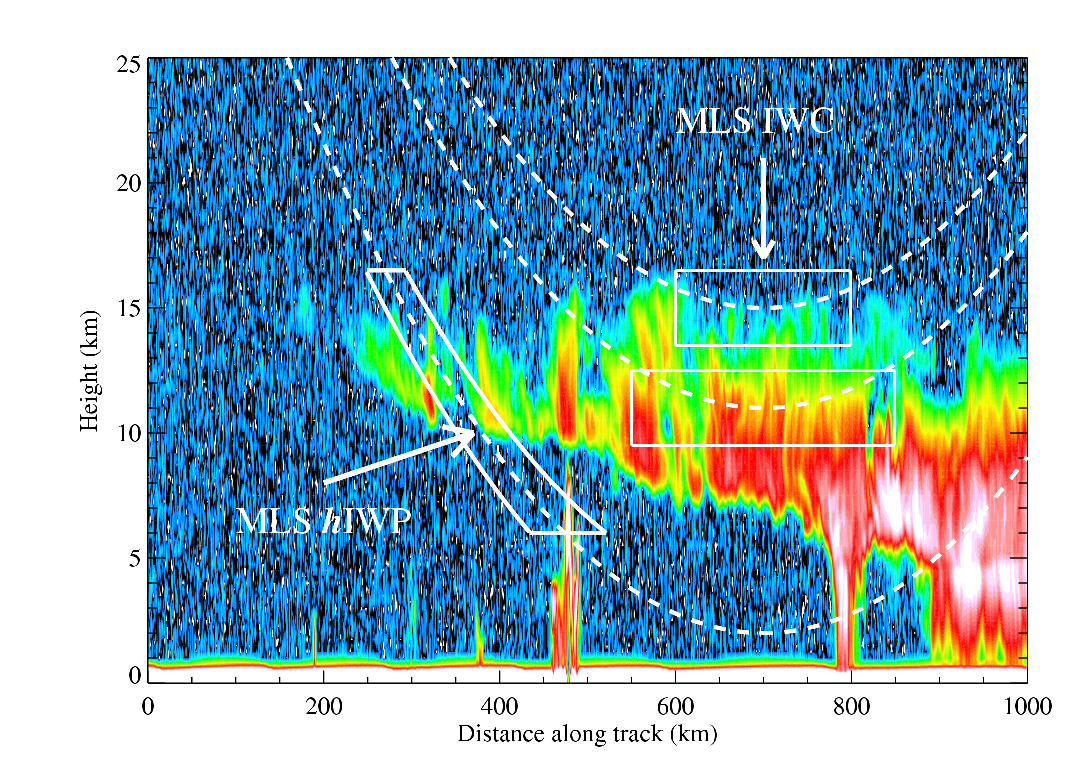
\includegraphics[width=\textwidth]{figures/iwp-figure-bitmap}
\caption{Diagram to illustrate the MLS IWC and IWP measurement. The
  dashed lines are the MLS tangential beams. At high tangent heights,
  the beams penetrate through the limb and become sensitive to a
  volume-averaged IWC, whereas at low tangent heights the MLS beams
  cannot penetrate through the limb due to strong gaseous absorption and
  become only sensitive to a partial slant column of IWP, with a shallow
  (\texttildelow3\degsym) angle, ``hIWP''.  Note that the actual volume of the
  air represented by hIWP is centered \texttildelow300\,km away from the
  tangent point, or \texttildelow2 profiles from the location of the nominal
  profile.}
\label{fig:IWPSketch}
\end{figure}

\begin{figure}
\includegraphics[width=\textwidth]{figures/IWP-240-v04-20-dataqual-JUL2009-v2}
\caption{MLS v4, v3 and v2 IWP comparisons for July 2009. 
  (a) Left: Probability density functions (PDF) (v4 (red), v3 (blue) and v2
  (green)) with dashed lines showing the corresponding noise levels
  (obtained by folding the negative IWP values about the origin) and the
  thin black lines representing the gaussian error function. (b) Right:
  Scatter plot of IWP v4 vs\. v2 (black points) with a dashed red lined
  indicating the 1:1 line and a linear fit to the data shown as a blue
  line.}
\label{fig:IWP}
\end{figure}

%%% Local Variables: 
%%% mode: latex
%%% TeX-master: "v4-x-report"
%%% End: 
 \speciestitle{Nitrous Oxide}{N\cs2O}{N2O}{%
\item[Useful range:] 68\,--\,0.46\,hPa
\item[Contact:] Alyn Lambert, \email{Alyn.Lambert@jpl.nasa.gov}}

\subsection*{Introduction}

\subsubsection*{Redefinition of the N\cs2O standard product for \thisv
  to use band 3 (190-GHz) signals}

The standard product for \thisv N\cs2O is taken from the 190-GHz
(``Core+R2'') retrieval (\texttt{N2O-190}) instead of the 640-GHz (``Core+R4B'')
retrieval (\texttt{N2O-640}) as used in previous versions.

Aging of the MLS ``band~12'' (640-GHz) signals was revealed by analysis
of housekeeping data during June-August 2013 which showed declining
output in counts, increasing radiance noise (variance) and also
increasing correlation between the band 12 radiance channels. As the
640\,GHz N\cs2O product began to show further deterioration in quality a
decision was made to turn off band 12 on August 6, 2013. Prior to that,
the level-2 processing stream for the N\cs2O standard product in v3.x
was switched to output the ``band~3'' (190-GHz, \texttt{N2O-190}) retrieval
on 7~June 2013 and later data for \texttt{N2O-640} are not recommended
for scientific use.

The 190-GHz N\cs2O data show slightly worse precision and resolution
compared to the 640-GHz retrievals. Data from \texttt{N2O-190} and
\texttt{N2O-640} have been compared from launch until the end of band 12
operations. There is a persistent high bias in \texttt{N2O-190} of
$>30\%$ at 100 hPa (although some seasonal variations are evident) and
we recommend that at this particular pressure level \texttt{N2O-190}
only be used in consultation with the MLS science team.  A smaller bias
of 5--10\% at 68\,hPa in \texttt{N2O-190} is seen compared to
\texttt{N2O-640}. From 46 to 3.2\,hPa the biases are less than 5\% (see
Figure~\ref{fig:N2O190640Comparison}).

\begin{figure}
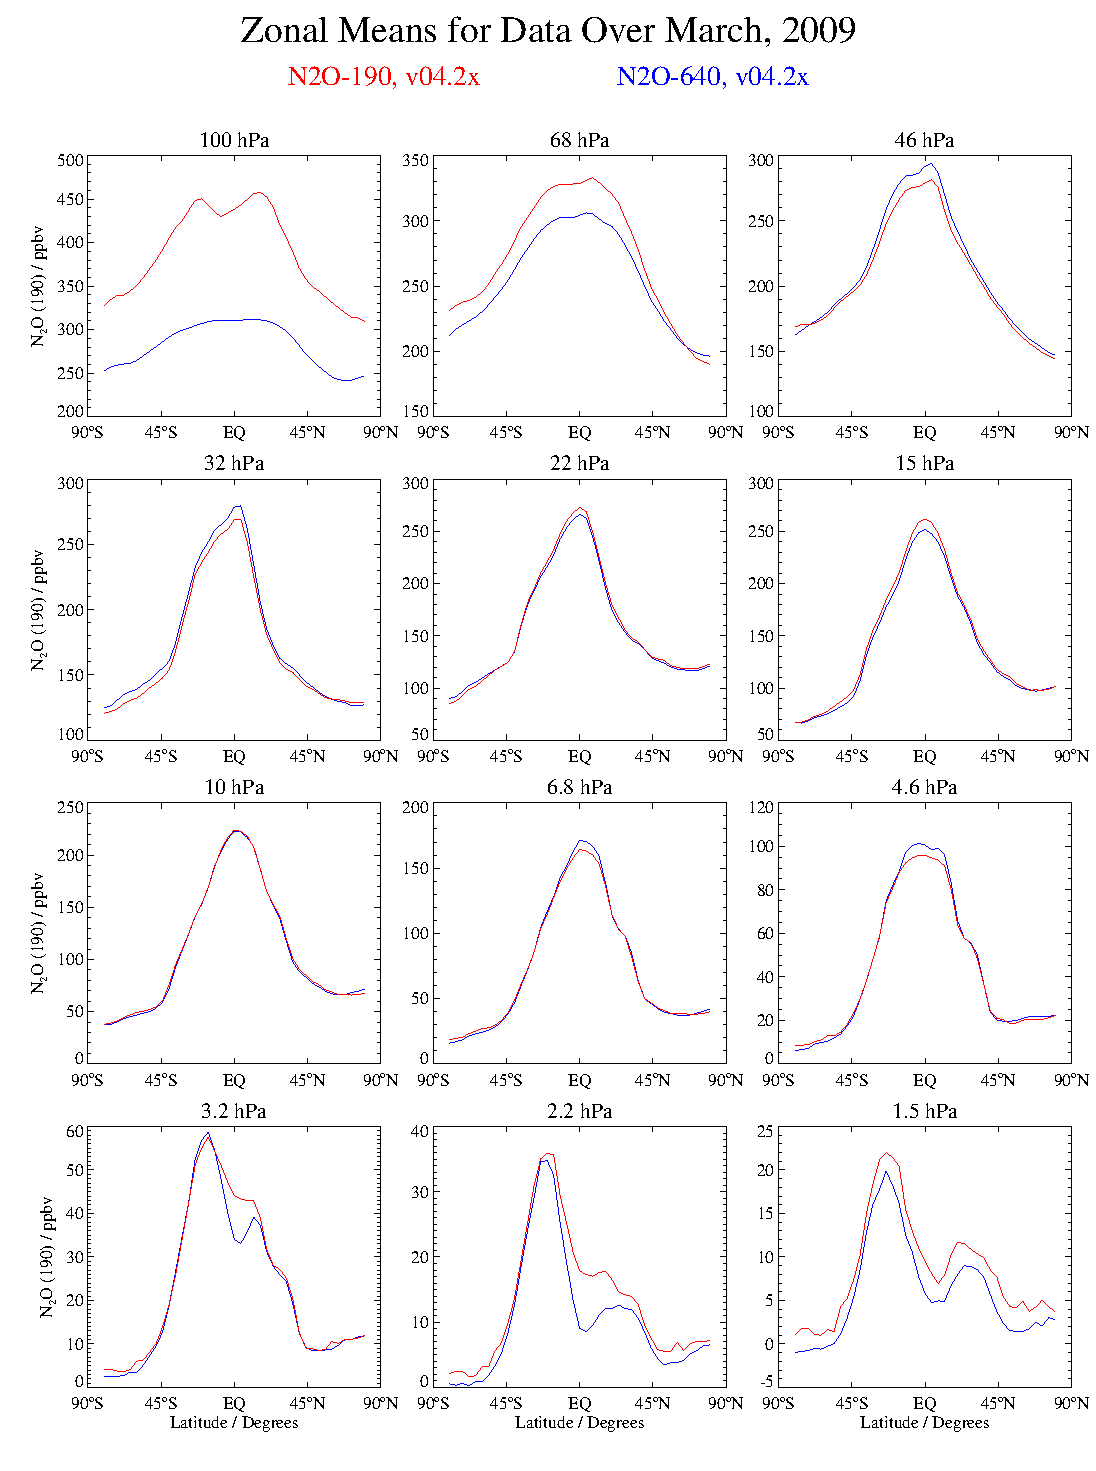
\includegraphics[width=\linewidth]{figures/InspectZM_2009m03_N2O-190-v04-2x_N2O-640-v04-2x_userHeightRange}
\caption{MLS \thisv \texttt{N2O-190} and \texttt{N2O-640} comparison for
  March 2009}
\label{fig:N2O190640Comparison}
\end{figure}

Other significant differences between the \thisv \texttt{N2O-190} and
\texttt{N2O-640} data such as the resolution, precision, recommended pressure levels, 
quality and convergence criteria are noted below.

The secondary \thisv N\cs2O 640-GHz product will be made available for
the period from launch until June 6, 2013 and stored in the
\texttt{L2GP-DGG} files in the \texttt{N2O-640} swath.  Details of the
retrieval method and validation results are presented in
\citep{LambertEtal07}.

\subsection*{Resolution}

\onestandardavk{N2O-190}{190\,GHz N\cs2O}

\onestandardavk{N2O-640}{640\,GHz N\cs2O}

The spatial resolution reported by the averaging kernel matrices is
shown in Figures~\ref{fig:AvkN2O-190} for the 190\,GHz measurements
and~\ref{fig:AvkN2O-640} for the 640\,GHz measurements (available in the
\texttt{L2GP-DGG} files for data prior to June~6, 2013).  For
\texttt{N2O-190}, the vertical resolution is 4\,--\,8\,km and the
horizontal along-track resolution is 300\,--\,600\,km.  For
\texttt{N2O-640}, the vertical resolution is 4\,--\,6\,km and the
horizontal along-track resolution is 300\,--\,600\,km over most of the
useful range of the retrievals.

The horizontal cross-track resolution is set by the 7\,km width of the
MLS 190-GHz field-of-view for all pressures. Note that the higher
frequency MLS 640-GHz measurements have a narrower 3\,km field-of-view.
The longitudinal separation of the MLS measurements is
10\degsym--\,20\degsym\ over middle and lower latitudes, with much finer
sampling in polar regions.

\subsection*{Precision}

Precision as defined here is the $1\sigma$ uncertainty in the retrieved
value calculated by the Level~2 algorithms and has been validated
against the scatter about the mean of coincident ascending/descending
MLS profile differences.  The estimated precision on a single retrieved
profile given in Tables~\ref{tab:N2OSummary} and~\ref{tab:N2O640Summary}
varies with height from \texttildelow15\,--\,20\,ppbv for \texttt{N2O-190} and
\texttildelow12\,--\,25\,ppbv for \texttt{N2O-640}.

The N\cs2O values at the 147\,hPa pressure level have a large a priori
influence and practically all precisions are flagged negative at this
level.

\subsection*{Accuracy}

The ``accuracy'' values given in Table~\ref{tab:N2O640Summary} were obtained 
for both v3.x N\cs2O products using the same detailed analyses 
presented for MLS \texttt{N2O-640} v2.2 data in
\citet{LambertEtal07} to quantify the systematic uncertainties
associated with the MLS instrument calibration, spectroscopic
uncertainty and approximations in the retrieval formulation and
implementation.  Accuracy for the \thisv N\cs2O data is 
expected to be little different from that established for v3.x. 


\subsection*{Data screening}
\label{sec:N2OScreening}
\begin{description}
\item[Pressure range (\texttt{N2O-190}):] \screeningrule{68\,--\,0.46\,hPa}
\item[Pressure range (\texttt{N2O-640}):] \screeningrule{100\,--\,0.46\,hPa}
\standardrangestatement\ In the upper stratosphere and lower
  mesosphere \thisv N\cs2O requires significant averaging for useful
  signals, but see the note under ``Artifacts'' for issues at pressures below
  0.1\,hPa.

\standardprecisionrule
\evenstatusrule

\item[Quality (\texttt{N2O-190}):] \qualityrule{1.3}
  A small fraction of \texttt{N2O-190} profiles (typically less than 4\%) will
  be discarded via this screening.

\item[Convergence (\texttt{N2O-190}):] \convergencerule{2.0}
  A fraction of the \texttt{N2O-190} data (typically less than 0.5\%) at this level
  will be discarded via this screening.

\item[Quality (\texttt{N2O-640}):] \qualityrule{1.4}
  A small fraction of \texttt{N2O-640} profiles (typically less than 0.5\%) will
  be discarded via this screening.

\item[Convergence (\texttt{N2O-640}):] \convergencerule{1.01}
  A fraction of the \texttt{N2O-640} data (typically less than 0.5\%) at this level
  will be discarded via this screening.

\item[Clouds:] \screeningrule{Clouds have little impact on the N\cs2O products at the recommended pressure levels. 
Ignore status bit 16 (high cloud) or bit 32 (low cloud) indicating the presence of clouds. See
artifacts for more details.}

\end{description}

\subsection*{Artifacts}

In addition to the large bias of the 190-GHz N\cs2O at 100\,hPa (not
removed by screening), there are occasional outliers at the highest
presure levels in \texttt{N2O-190} and \texttt{N2O-640} products. 
Very thick clouds in the tropics produce a low rate of artifacts in the \thisv N\cs2O
products since improvements in the handling of radiances affected by
clouds have reduced the frequency of outliers compared to previous
versions. The cloud bits of the \texttt{Status} field are too blunt a
tool to identify these rare cases, needlessly discarding reasonable data.
Screening using the convergence
and quality fields (see above) is recommended to remove the majority of
these data points. 

The retrieval restricts N\cs2O values to be greater than
$-40\,\text{ppbv}$ (approximately three times the retrieval noise level
in the recommended pressure range) in order to prevent problems in the
minimization search process.  The low bound is applied at all levels,
but it is only evident in the data for pressures less than 0.1\,hPa,
where the vertical smoothing is relaxed and the retrieval noise becomes
comparable to the magnitude of the low bound value.  Accordingly,
statistical averaging of the data (zonal means or longer time periods)
cannot be applied successfully for pressures at and less than 0.1\,hPa
as the $-40\,\text{ppbv}$ hard limit introduces a positive bias in any
average.

\subsection*{Review of comparisons between MLS N\cs2O  versions and other datasets}

Average values for \thisv 190-GHz N\cs2O are up to 10\% smaller than in v2.2 for the
100 and 68\,hPa pressure levels, and within a few percent for pressures greater than 46\,hPa 
(see Figure~\ref{fig:N2O190Comparison}). Differences between \thisv 190-GHz N\cs2O and
v3.3 are less than a few percent at all levels.

\begin{figure}
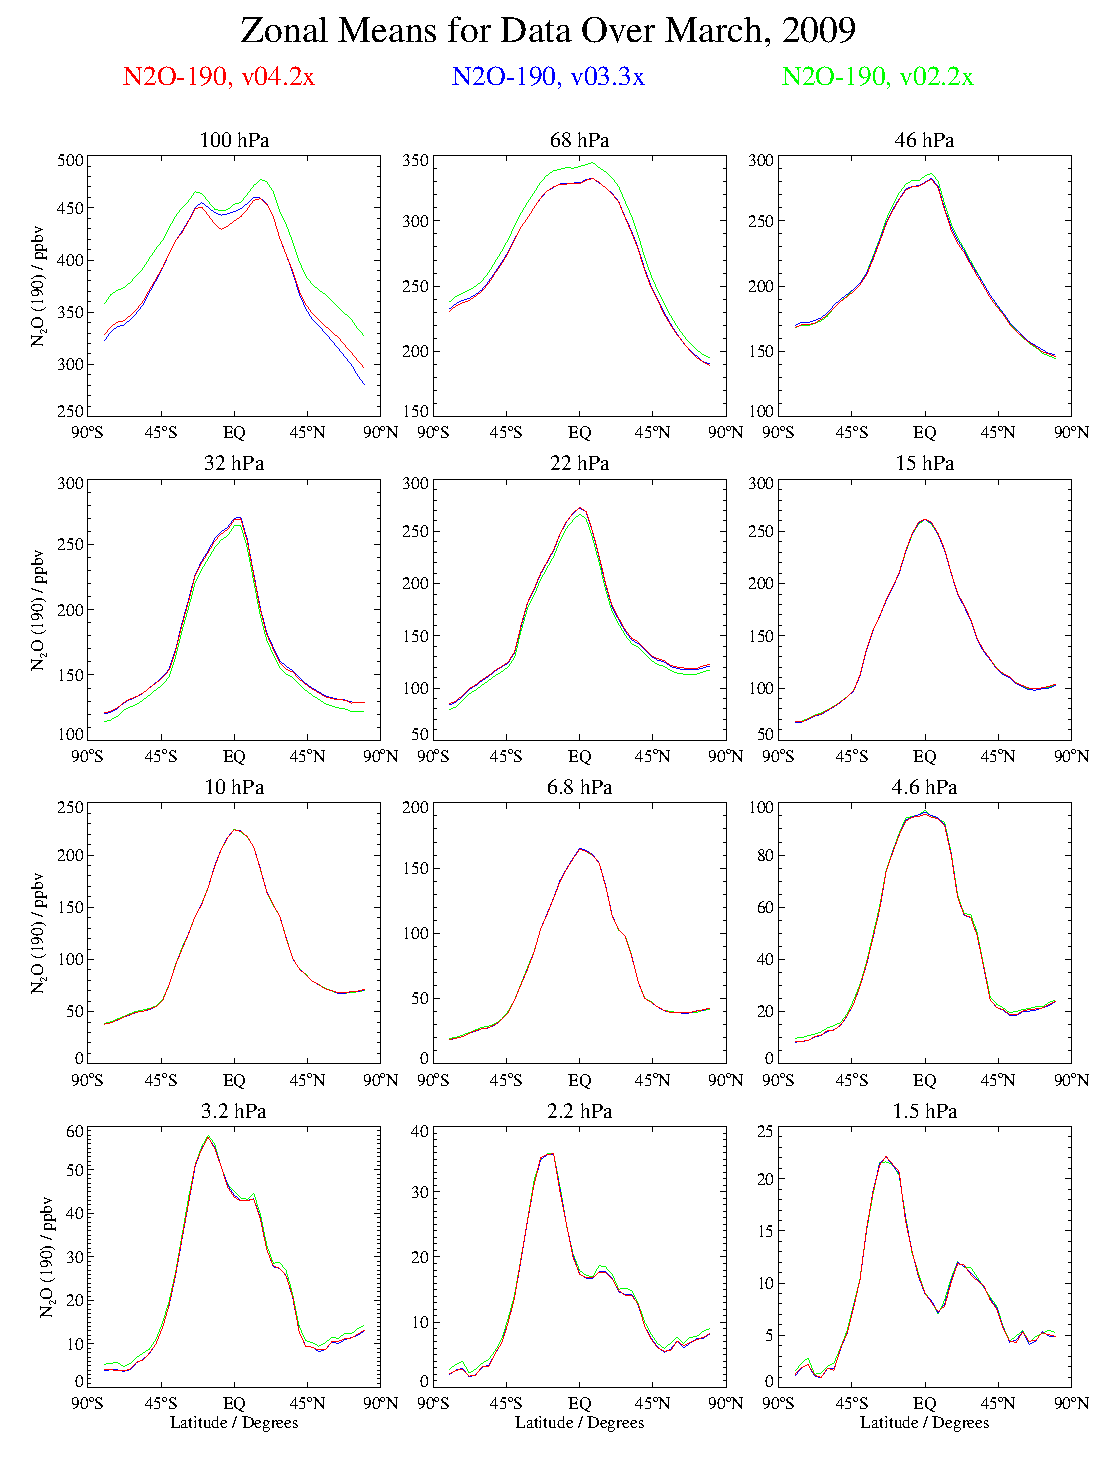
\includegraphics[width=\linewidth]{figures/InspectZM_2009m03_N2O-190-v04-2x_N2O-190-v03-3x_N2O-190-v02-2x_userHeightRange}
 \caption{MLS v4.2 190-GHz N\cs2O compared to v2.2 and v3.3 for March 2009}
\label{fig:N2O190Comparison}
\end{figure}

Average values for \thisv 640-GHz N\cs2O are 20\% larger than in v2.2
for the 100\,hPa pressure level, up to 10\% smaller at the
46\,--\,32\,hPa levels, and within 5\% for pressures greater than
22\,hPa (see Figure~\ref{fig:N2O640Comparison}). Differences between
\thisv 640-GHz N\cs2O and v3.3 are less than a few percent at all
levels. Unlike the \texttt{N2O-190} product, the \texttt{N2O-640}
product is recommended for scientific use at 100\,hPa.

Apart from the differences noted above, the MLS \thisv 640 GHz N\cs2O is
similar to the MLS v2.2 product described and validated in
\citet{LambertEtal07}.  Comparisons of v2.2 640 GHz N\cs2O with
coincident measuremements by ACE-FTS, Odin/SMR, and Envisat/MIPAS and
balloon borne observations are shown in \citet{LambertEtal07}.  A
revised validation paper for N\cs2O is not planned in the near future
and users are encouraged to read \citet{LambertEtal07} for more
information.

\begin{figure}
  \includegraphics[width=\linewidth]{figures/InspectZM_2009m03_N2O-640-v04-2x_N2O-640-v03-3x_N2O-640-v02-2x_userHeightRange}
 \caption{MLS v4.2 640 GHz N\cs2O compared to v2.2 and v3.3 for March 2009}
\label{fig:N2O640Comparison}
\end{figure}

\subsection*{Desired improvements for future data version(s)}

Retrievals of N\cs2O to pressures greater than 147\,hPa \emph{may} be
possible in later versions from the 190-GHz observations.

\begin{table}[b]
  \caption{Summary of MLS \thisv N\cs2O (\texttt{N2O-190}) product.}\vspace{0.5ex}
\label{tab:N2OSummary}
\begin{minipage}{\linewidth}
\centering\begin{tabular}{ccccccl}
\toprule
\parbox[m]{15mm}{\centering\textbf{Region}} &
\parbox[m]{24mm}{\centering\textbf{Resolution\\ Vert. $\times$ Horiz.}} &
\multicolumn{2}{c}{\parbox[m]{18mm}{\centering\textbf{Precision\footnote{Precision on individual profiles}}}} &
\multicolumn{2}{c}{\parbox[m]{15mm}{\centering\textbf{Accuracy}}} &
\textbf{Comments} \\
\textbf{hPa} & \textbf{km} &  \textbf{ppbv} & \textbf{\%} & \textbf{ppbv} & \textbf{\%} & \\
\midrule
$\leq$0.33   & ---                 & ---   & ---       & --- & --- & Unsuitable for scientific use \\   
0.46         &  11.0 $\times$  655 &   15  & $>$100 & 0.5 & 16 & \\ 
0.68         &   9.7 $\times$  540 &   17  & $>$100 & 0.6 & 16 & \\ 
1.0          &   8.6 $\times$  440 &   18  & $>$100 & 0.8 & 16 & \\ 
2.2          &   7.3 $\times$  340 &   19  &   64   & 2.4 & 18 & \\ 
4.6          &   6.5 $\times$  285 &   17  &   23   &  3  &  8 & \\ 
10           &   6.0 $\times$  265 &   16  &   12   &  5  &  6 & \\ 
22           &   5.6 $\times$  305 &   15  &    9   & 10  &  7 & \\ 
46           &   4.9 $\times$  385 &   14  &    7   & 16  &  7 & \\ 
68           &   5.4 $\times$  420 &   16  &    6   & 20  &  8 & \\
100          &   3.8 $\times$  500 &   20  &    7   & $>50$  & $>$30 & Consult with MLS science team\\ 
147          & ---                 & ---   & ---    & --- & ---& Unsuitable for scientific use \\   
$\geq$215    & ---                 & ---   & ---    & --- & ---& Not retrieved \\
\bottomrule
\end{tabular}
\end{minipage}
\end{table}

\begin{table}[b]
  \caption{Summary of MLS \thisv N\cs2O (\texttt{N2O-640}) product.}\vspace{0.5ex}
\label{tab:N2O640Summary}
\begin{minipage}{\linewidth}
\centering\begin{tabular}{ccccccl}
\toprule
\parbox[m]{15mm}{\centering\textbf{Region}} &
\parbox[m]{24mm}{\centering\textbf{Resolution\\ Vert. $\times$ Horiz.}} &
\multicolumn{2}{c}{\parbox[m]{18mm}{\centering\textbf{Precision\footnote{Precision on individual profiles}}}} &
\multicolumn{2}{c}{\parbox[m]{15mm}{\centering\textbf{Accuracy}}} &
\textbf{Comments} \\
\textbf{hPa} & \textbf{km} &  \textbf{ppbv} & \textbf{\%} & \textbf{ppbv} & \textbf{\%} & \\
\midrule
$\leq$0.33   & ---                 & ---   & ---       & --- & --- & Unsuitable for scientific use \\   
0.46         &   8.9 $\times$  530 &   12  &  $>$100   & 0.5 & 16  & \\     
0.68         &   7.4 $\times$  430 &   13  &  $>$100   & 0.6 & 15  & \\     
1.0          &   6.2 $\times$  345 &   14  &  $>$100   & 0.6 & 12  & \\    
2.2          &   4.8 $\times$  300 &   15  &   49      & 1.2 &  9  & \\    
4.6          &   4.1 $\times$  295 &   14  &   18      &  3  &  9  & \\          
10           &   3.9 $\times$  360 &   13  &   10      &  7  &  9  & \\          
22           &   4.2 $\times$  410 &   14  &    8      & 19  & 13  & \\          
46           &   4.4 $\times$  495 &   16  &    7      & 32  & 14  & \\          
68           &   5.5 $\times$  555 &   20  &    8      & 32  & 13  & \\          
100          &   5.2 $\times$  610 &   25  &    9      & 70  & 25  & \\          
147          & ---                 & ---   & ---       & --- & --- & Unsuitable for scientific use \\   
$\geq$215    & ---                 & ---   & ---       & --- & --- & Not retrieved \\
\bottomrule
\end{tabular}
\end{minipage}
\end{table}

%%% Local Variables:  
%%% mode: latex 
%%% TeX-master: "v4-x-report" 
%%% End:  

 \speciestitle{Ozone}{O\cs3}{O3}{%
\item[Useful range:] 261\,--\,0.02\,hPa  
\item[Contact:] Lucien Froidevaux (stratosphere/mesosphere), 
  \email{Lucien.Froidevaux@jpl.nasa.gov} \\ 
  Michael Schwartz (upper troposphere), 
  \email{Michael.J.Schwartz@jpl.nasa.gov}}
 
\subsection*{Introduction} 

As is the case with previous versions, the \thisv standard O\cs3
product is taken from a retrieval using 240-GHz radiances, 
providing sensitivity from the upper troposphere into the mesosphere.
In \thisv, an optimized retrieval phase for production of the O\cs3
standard product has been added prior to the phase that uses
240-GHz radiances to produce the standard  carbon monoxide and nitric 
acid products.  Table~\ref{tab:O3Summary}
summarizes typical O\cs3 resolution, precision, and systematic uncertainty
estimates as a function of pressure.  Papers describing detailed
validation of the MLS v2.2 product and comparisons with other data sets
were published in a special Aura validation issue of the {\it Journal of
  Geophysical Research}, see
\citep{FroidevauxEtal08O3,JiangYEtal07,LiveseyEtal08}.  In the
stratosphere and above, \thisv ozone profiles are very similar to the
v2.2 and \prevvSlash profiles, so the stratospheric results from the
above references will generally hold for the product.  Initial
documentation of changes, improvements, and issues with \thisv data are
discussed here, including data screening criteria.  Recommended
screening is less complex than it was for \prevvSlash data and is again
primarily based on thresholds for \texttt{Quality}, and
\texttt{Convergence}, as was the case for v2.2.  Ozone profile behavior
has been improved, with reduction of vertical oscillations in the
low-latitude UTLS and reduction of sensitivity to thick clouds, 
through changes in the spectral form used to model cloud impacts on the
MLS radiances, through tightening of vertical smoothing at pressures greater
than or equal to 68\,hPa (leading to an increase in averaging kernel
FWHM by a factor of \texttildelow1.15) and through retrieval of an independent,
spectrally-flat baseline over the ozone band for each limb view to
better account for cloud inhomogeneity.

 
In addition to the swath \texttt{O3}, which is the O\cs3 profile on 55
pressure surfaces, the \texttt{L2GP-O3} files contain a swath,
\texttt{O3~column}, which is the integrated stratospheric column down to
the thermal tropopause (WMO definition) calculated from MLS temperature.
The MLS temperature profiles from which the WMO
tropopause is determined are not screened per the instructions of
section~\ref{sec:StandardTemperature} and users may wish to
reject columns for which standard screening rejects the corresponding
temperature profile.

\subsection*{Comparison of \thisv with past data versions}  

The vertical retrieval grid has not changed from \prevvSlash; between
316\,hPa and 1\,hPa, \thisv ozone profiles are retrieved on 12 surfaces
per decade, a grid twice as fine as the 6-level-per-decade grid used in
v2.2 Tightened vertical smoothing has degraded vertical resolution in
\thisv from the upper troposphere to 68\,hPa by \texttildelow15\%.
Table\ref{tab:O3Summary} summarizes resolution, precision, and accuracy
estimates.
 
\begin{figure} 
  \centering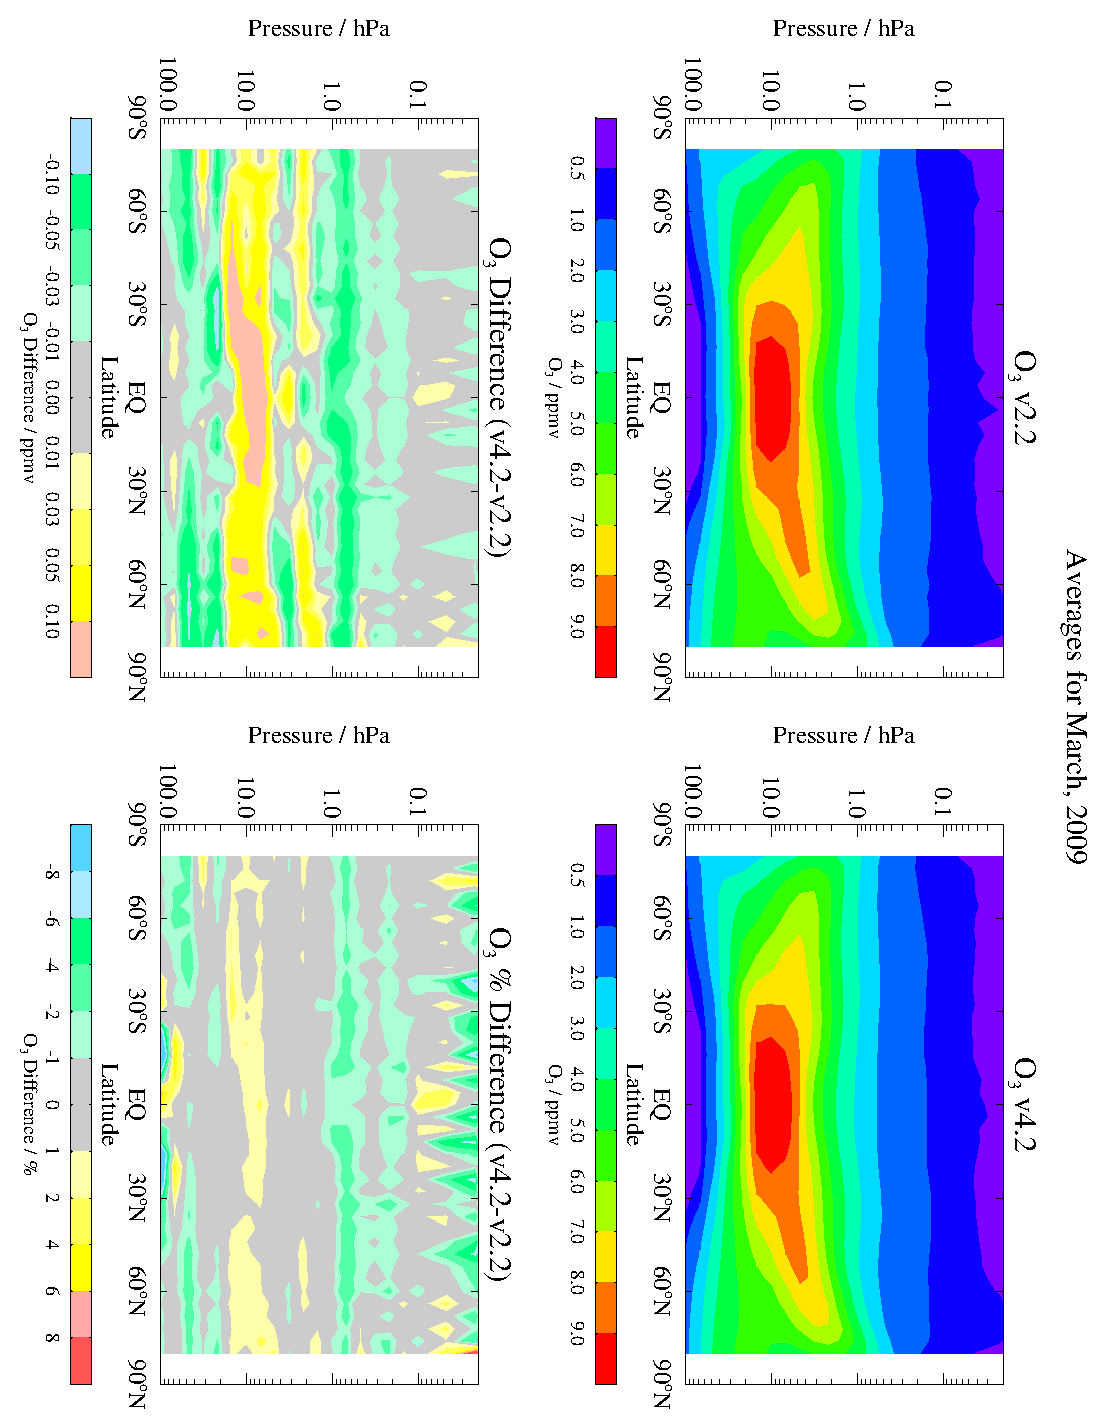
\includegraphics[angle=90,width=\linewidth]{figures/Fig-O3-ZMContours-v2-2-v4-2_2009m03_StratMes}
\caption{Zonal averages for stratospheric and mesospheric MLS ozone
  profiles during March, 2009, showing the MLS v2.2 ozone mixing ratio
  contours (top left panel), the \thisv contours (top right panel), and
  their differences in ppmv (\thisv minus v2.2, bottom left panel) and
  percent (\thisv minus v2.2 versus v2.2, bottom right panel). }
\label{fig:MLSv2v4O3ContourStrat} 
\end{figure} 

\begin{figure} 
\centering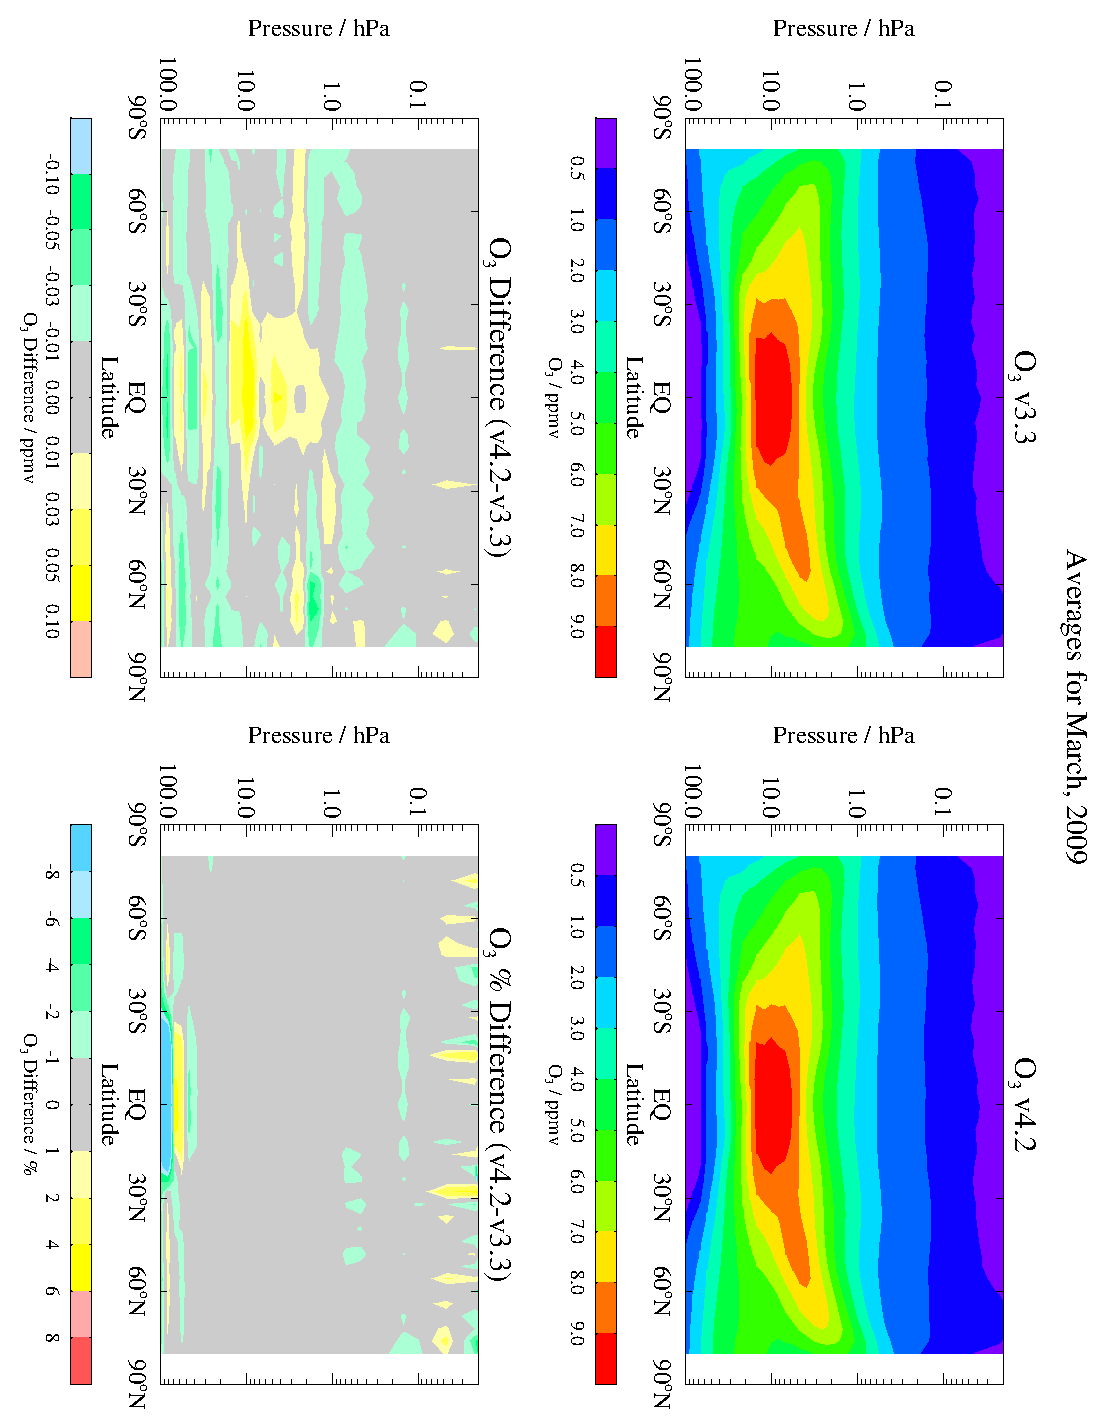
\includegraphics[angle=90,width=\linewidth]{figures/Fig-O3-ZMContours-v3-3-v4-2_2009m03_StratMes}
\caption{Zonal averages for stratospheric and mesospheric MLS ozone
  profiles during March, 2009, showing the MLS v3.3 ozone mixing ratio
  contours (top left panel), the \thisv contours (top right panel), and
  their differences in ppmv (\thisv minus v3.3, bottom left panel) and
  percent (\thisv minus v3.3 versus v3.3, bottom right panel). }
\label{fig:MLSv3v4O3ContourStrat} 
\end{figure} 
 
\begin{figure} 
\centering\includegraphics[angle=90,width=\linewidth]{figures/Fig-O3-ZMContours-v2-2-v4-2_2009m03_UTLS}
\caption{Zonal averages for UTLS MLS ozone profiles during March, 2009,
  showing the MLS v2.2 ozone mixing ratio contours (top left panel), the
  \thisv contours (top right panel), and their differences in ppmv
  (\thisv minus v2.2, bottom left panel) and percent (\thisv minus v2.2
  versus v2.2, bottom right panel). }
\label{fig:MLSv2v4O3ContourUTLS} 
\end{figure} 

\begin{figure} 
\centering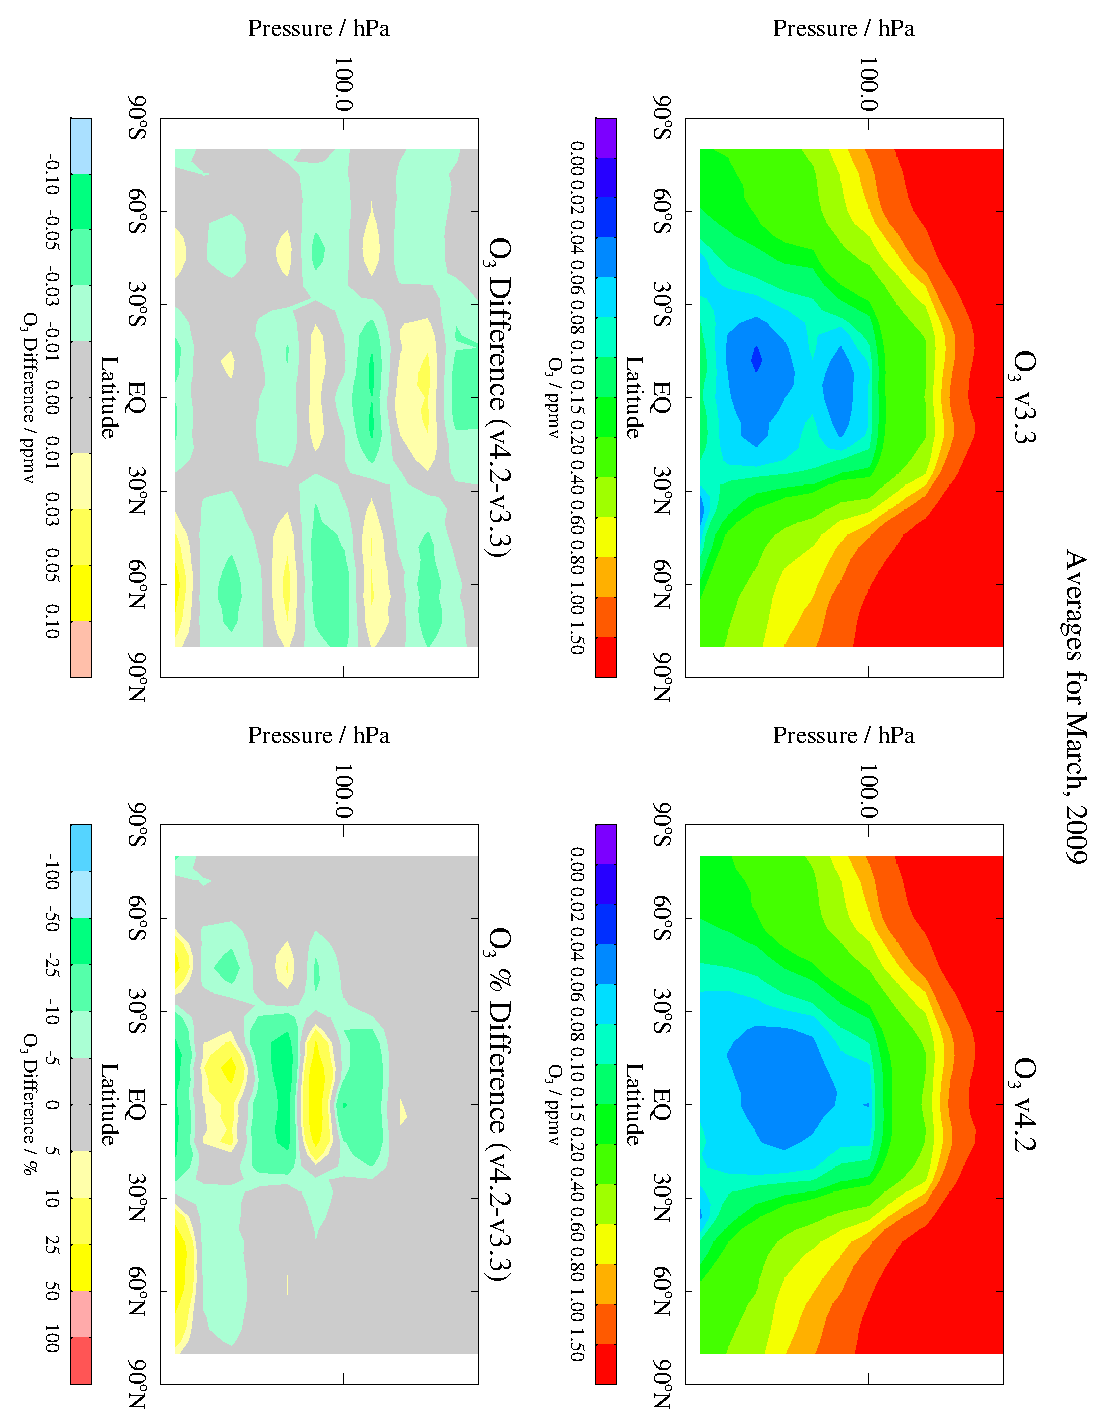
\includegraphics[angle=90,width=\linewidth]{figures/Fig-O3-ZMContours-v3-3-v4-2_2009m03_UTLS}
\caption{Zonal averages for UTLS MLS ozone profiles during March, 2009,
  showing the MLS v3.3 ozone mixing ratio contours (top left panel), the
  \thisv contours (top right panel), and their differences in ppmv
  (\thisv minus v3.3, bottom left panel) and percent (\thisv minus
  v3.3 versus v3.3, bottom right panel). }
\label{fig:MLSv3v4O3ContourUTLS} 
\end{figure} 

Figures \ref{fig:MLSv2v4O3ContourStrat} and
\ref{fig:MLSv3v4O3ContourStrat} show zonally-averaged stratospheric and
mesospheric field comparisons between data versions for the (full) month
of March, 2009, for properly screened profiles only; mean differences
(ppmv and percent) are also shown. Similar plots focusing on the UTLS
are provided in Figures \ref{fig:MLSv2v4O3ContourUTLS} and
\ref{fig:MLSv3v4O3ContourUTLS}.  Average ozone mixing ratio values
(e.g., for monthly means) have typically not changed by more than 1 to
2\% for pressures less than 100\,hPa. In the tropical UTLS (most
notably), the new dataset is improved. Specifically, we show average
UTLS profiles during March, 2009 from three data versions for 0\degsym
--\,10\degsym N in Figure \ref{fig:MLSO3kinkUTLS}. The new version shows less
oscillatory behavior in the mean profiles, in comparison to the previous
version (v3.3 on the same retrieval grid), although small oscillations
are still present; certain months and latitude regions exhibited larger
effects (in the previous data version) than those shown in the above
figure. 

\begin{figure} 
\centering\includegraphics[angle=90,width=0.6\linewidth]{figures/Fig-O3_kink_v4_v3_v2_2009_March_0-10N}
\caption{Zonal means from equator to 10\degsym N during March, 2009,
  showing the average behavior of ozone profiles for MLS v2.2, v3.3, and
  \thisv, as indicated by the color-coded legend.}
\label{fig:MLSO3kinkUTLS} 
\end{figure} 

Figure~\ref{fig:MLSO3histUTLS} shows histograms of tropical UTLS v04.20
and v03.30 ozone for all of 2005.  V04.20 ozone unscreened (blue) and
screened (green) histograms are quite similar to one another, with only
small reductions in scatter in the screened case.  V3.3 has
significantly broader distributions in the troposphere than v04.20, both
in the widths of the central peaks and in the tails of the
distributions.  While screened v3.3 (cyan) has reduced tails of
cloud-impacted outliers compared to unscreened (red), these tails are 
clearly reduced in \thisv even before screening. The reduced tropical vertical oscillation
seen in Figures~\ref{fig:MLSv3v4O3ContourUTLS} and~\ref{fig:MLSO3kinkUTLS}  is reflected in
the shifts of the histogram peaks between versions, with higher \thisv
values at 121\,hPa and lower values at 82, 100, 147, 178 and 316\,hPa.
The 316-hPa level of \thisv, though not currently recommended for
general scientific use, is under evaluation.
\begin{figure} 
\centering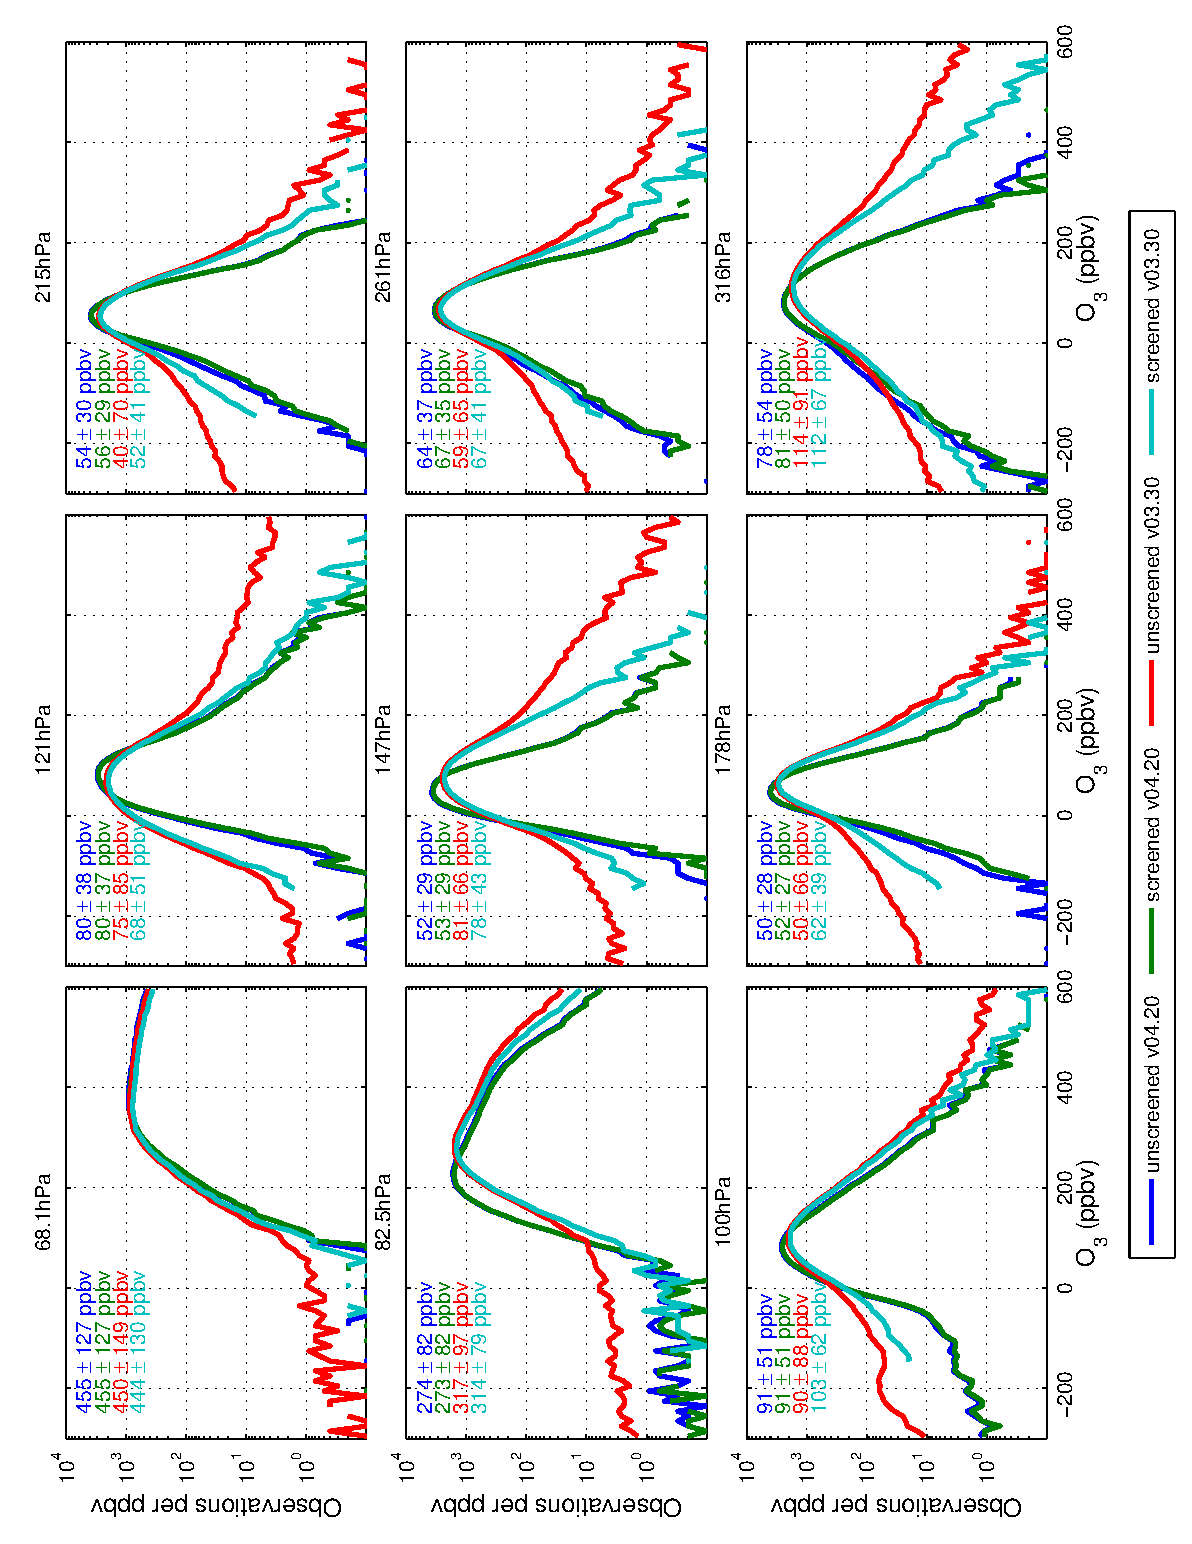
\includegraphics[angle=-90,width=0.8\linewidth]{figures/O3_v4v3_hist_9lev_tropics}
\caption{Histograms of screened and unscreened v04.20 and v03.30 ozone
  for the 2005 tropical average (20$^\circ$\,S--20$^\circ$\,N).  }
\label{fig:MLSO3histUTLS} 
\end{figure} 

%At low latitudes, zonal-mean \thisv tends to be \texttildelow10\,ppbv larger than v2.2 from 215\,hPa to
%100\,hPa, while at higher latitudes, the v2.2/\thisv relationship tends
%to switch signs, with \thisv higher than v2.2 at 316\,hPa and 147\,hPa,
%and lower at 215\,hPa and 100\,hPa (see Figure \ref{fig:MLSv2v3O3ContourUTLS}). 

\paragraph*{Ozone Columns}
Changes in the MLS stratospheric ozone columns between \prevvSlash and
\thisv are quite small; typical daily zonal averages are within one
percent, with a tendency towards slightly lower values (but within about
1\%) in the new data version.  Only one stratospheric column swath,
using a tropopause derived from MLS temperature, is calculated by the
\thisv O\cs3 retrieval.  The column based upon the GEOS-5 tropopause is
no longer routinely produced.
\subsection*{Resolution} 

%\onestandardavk{O3_HR}{O\cs3} 
 
\begin{figure} 
  \centering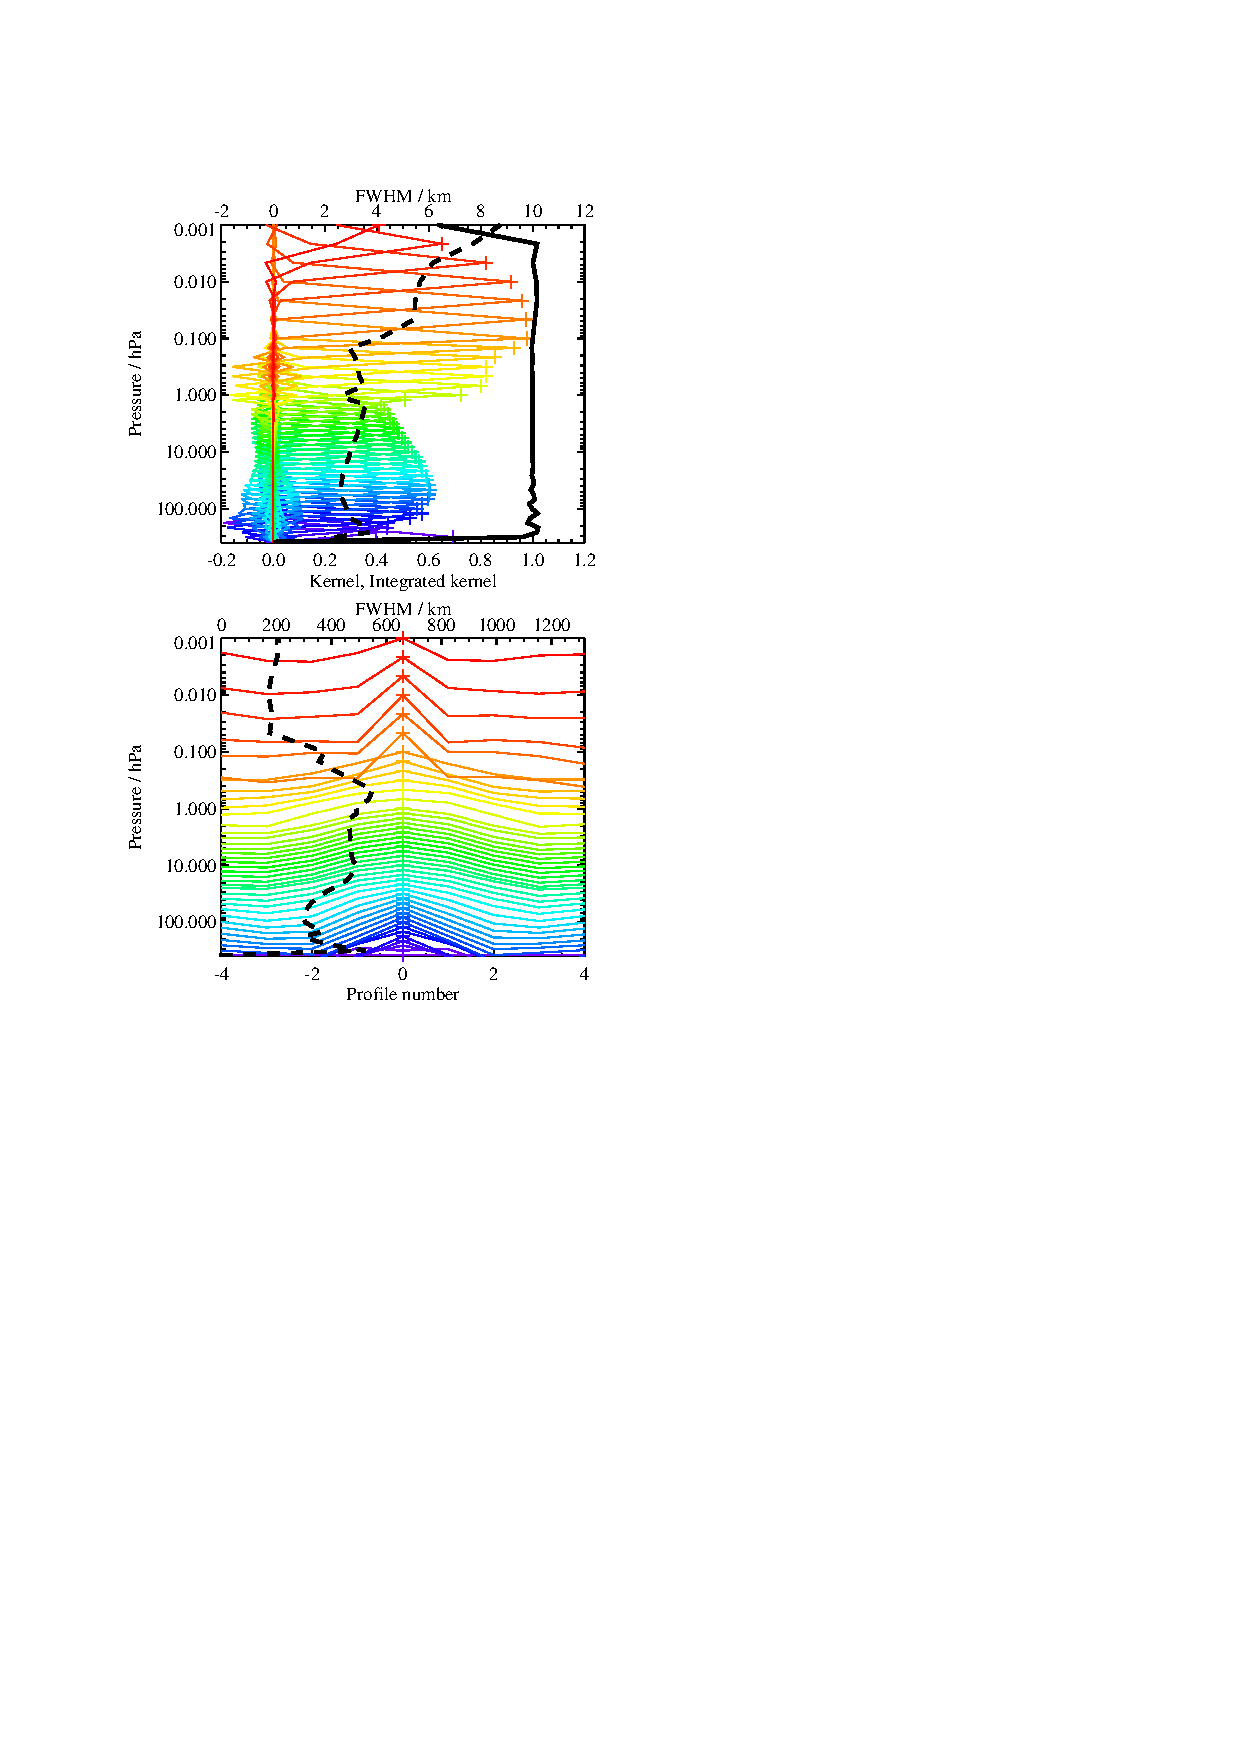
\includegraphics[width=0.5\linewidth]{figures/avk-O3_HR-35N-292a-OzoneOnly}
  \caption{Typical two-dimensional (vertical and horizontal along-track)
    averaging kernels for the MLS \thisv O\cs3 at 35\degsym\,N;
    variation in the averaging kernels is sufficiently small that these
    are representative of typical profiles.  Colored lines show the
    averaging kernels as a function of MLS retrieval level, indicating
    the region of the atmosphere from which information is contributing
    to the measurements on the individual retrieval surfaces, which are
    denoted by plus signs in corresponding colors.  The dashed black
    line indicates the resolution, determined from the full width at
    half maximum (FWHM) of the averaging kernels, approximately scaled
    into kilometers (top axes).  (Upper) Vertical averaging kernels
    (integrated in the horizontal dimension for five along-track
    profiles) and resolution.  The solid black line shows the integrated
    area under each kernel (horizontally and vertically); values near
    unity imply that the majority of information for that MLS data point
    has come from the measurements, whereas lower values imply
    substantial contributions from a priori information.  (Lower)
    Horizontal averaging kernels (integrated in the vertical dimension)
    and resolution.  The averaging kernels are scaled such that a unit
    change is equivalent to one decade in pressure.}
\label{fig:avkO3Strat} 
\end{figure} 
 
\begin{figure} 
  \centering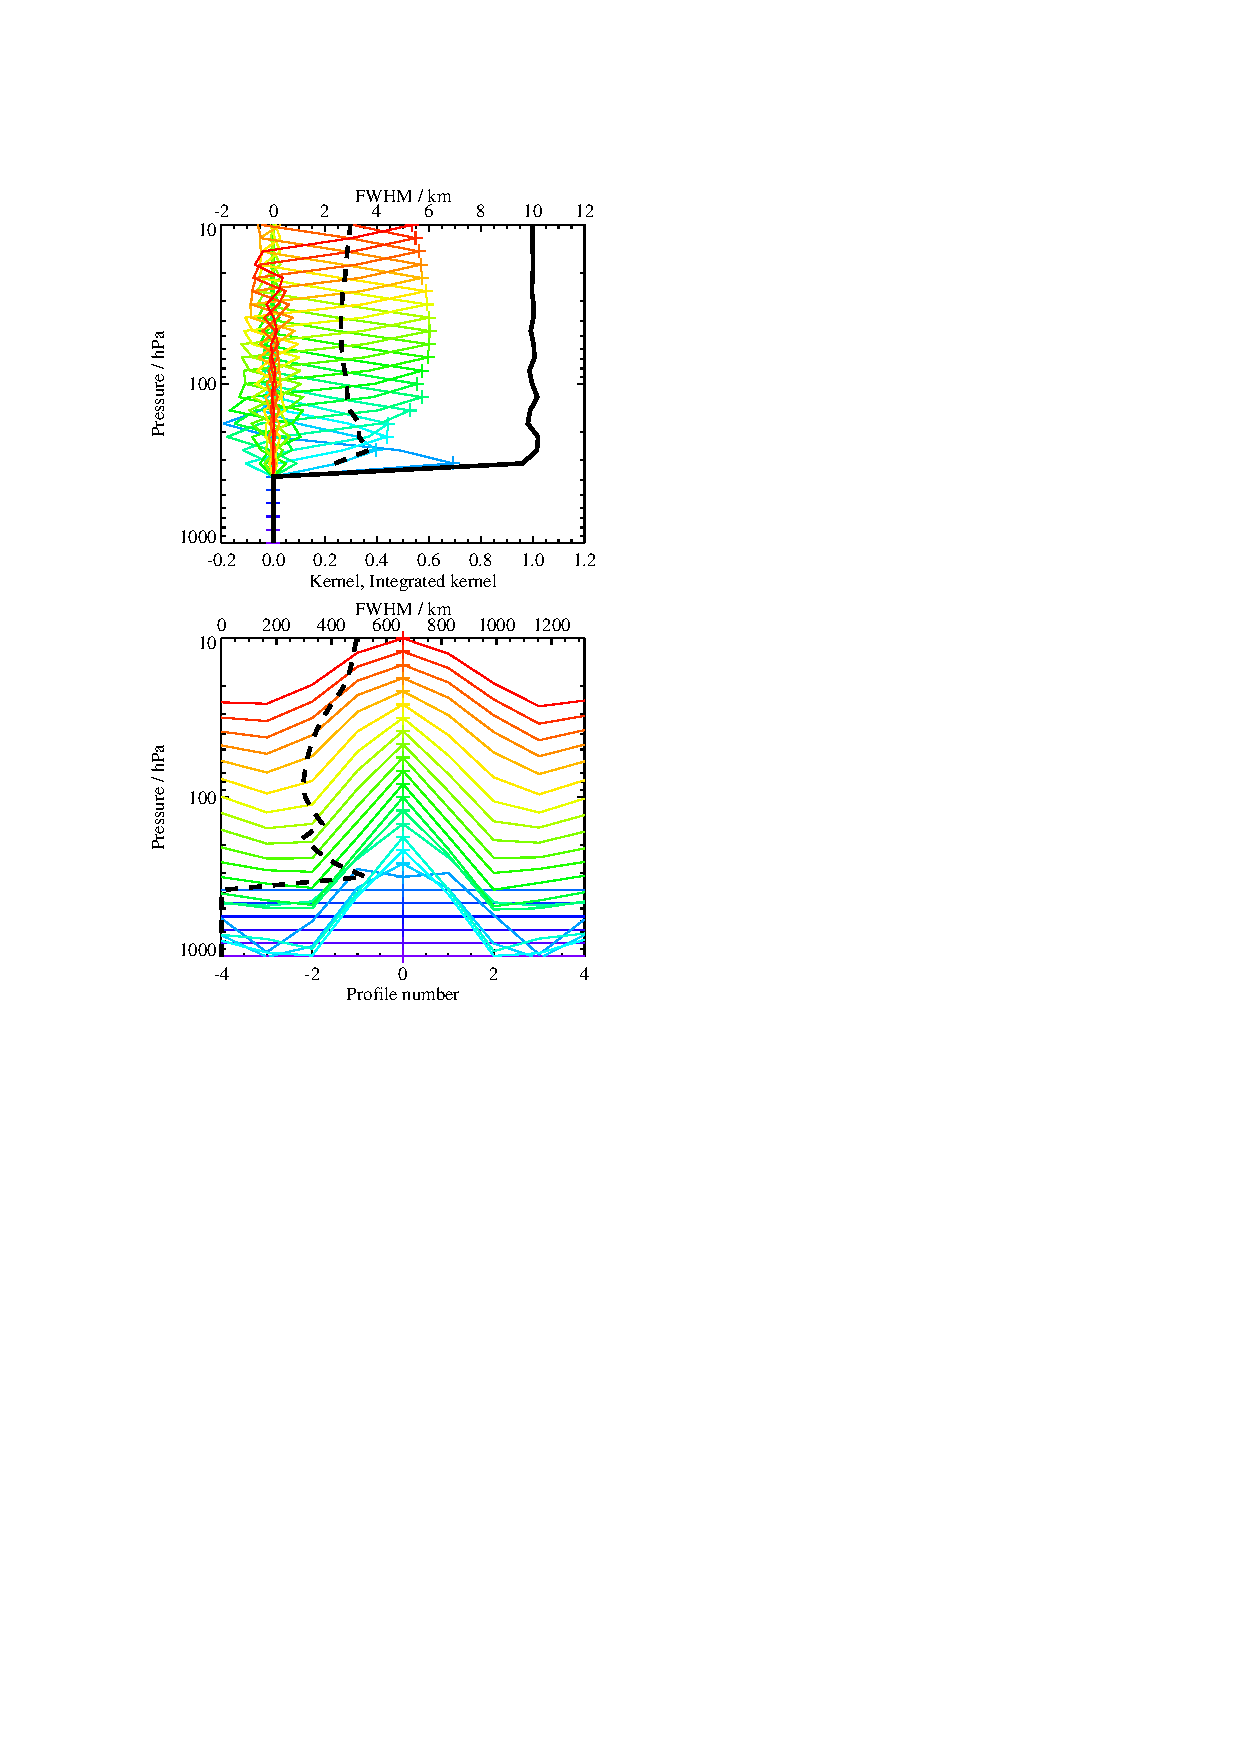
\includegraphics[width=0.5\linewidth]{figures/avk-O3_HR-35N-292a-UTLS-OzoneOnly}
  \caption{As for \protect{\ref{fig:avkO3Strat}} but zooming in on the
    upper troposphere and lower stratosphere region.}
\label{fig:avkO3UTLS} 
\end{figure} 
 
Typical resolution values are provided in the summary
Table~\ref{tab:O3Summary}.  The cross-track resolution is set by the
6\,km width of the MLS 240\,GHz field of view.  Daily longitudinal
separation of MLS measurements, set by the Aura orbit, is
10\degsym--\,20\degsym\ over middle and lower latitudes, with much finer
sampling at the highest latitudes sampled in each hemisphere.
 
\subsection*{Precision} 
 
As found previously, the Level~2 precision values are often slightly lower than 
the scatter observed in a narrow latitude band centered 
around the equator (where atmospheric variability is expected to be small) or
obtained from a comparison between ascending and descending coincident
MLS profiles.
 
Negative precision values for ozone occur for almost every data
point at pressures smaller than 0.01\,hPa, indicating increasing
influence from the \emph{a priori}, although some MLS information exists
(e.g., regarding average day/night differences) into the uppermost
mesosphere and lower thermosphere.  Generally, however, we recommend
that scientific studies be restricted to pressures of 0.02\,hPa or
larger.
 
\paragraph*{Column values} The estimated precisions for the v4.2 MLS 
column ozone abundances down to pressures of 100 to 215\,hPa are 2\% or less.  
The typical empirical precision in the columns based on (1-$\sigma$)
variability in the tropics is 2 to 3\%.  
 
\subsection*{Accuracy}
 
The accuracy estimates shown in Table~\ref{tab:O3Summary} are from an
analysis which propagated estimated systematic errors in MLS
calibration, spectroscopy, etc., through the v2.2 measurement system.
Results using the v4.2 algorithms are not expected to differ
significantly.  The values shown here are intended to represent
2$\sigma$ estimates of accuracy.  Comparison of MLS O\cs3 with
well-established data sets shows no evidence of significant biases.
For more
details, see the MLS validation papers by \citet{FroidevauxEtal08O3},
\citet{JiangYEtal07}, and \citet{LiveseyEtal08}, as well as references
therein; some more recent references relevant to MLS ozone are available
on the MLS website under ``Publications''.  Future validation studies
using v4.2 data will focus on longer-term changes (for which good
stability is being observed versus other reliable measurements) and on
the UTLS region.
 
\paragraph*{Column values}
Sensitivity tests using systematic changes in various parameters that
could affect the accuracy of the MLS retrievals lead to possible biases
($2\sigma$ estimates) of about 4\%, as an estimated accuracy for the MLS
column values (from integrated MLS ozone profiles down to 100, 147, and
215\,hPa).  See also the (v2.2) validation papers (and subsequent
ozone-related publications, e.g., available from the MLS website) for
results on column ozone comparisons versus satellite, sonde, and lidar
data.
 
\subsection*{Data screening} 
\label{sec:O3Screening}
\begin{description} 
 
\item[Pressure range:] \screeningrule{261\,--\,0.02\,hPa.}
  \standardrangestatement 
  \standardprecisionrule
  \evenstatusrule
\item[Quality:] \qualityrule{1.0}
\item[Convergence:] \convergencerule{1.03}
\item[Clouds:] \screeningrule{Scattering from thick clouds can lead to
    more systematic effects in the UTLS.}  Most of the affected profiles
  are removed by the \texttt{Quality} and \texttt{Convergence} screening
  recommendations (although \texttt{Convergence} issues occur only
  rarely).

  One should \emph{reject} profiles with odd \texttt{Status} \emph{or}
  even \texttt{Status} profiles with \texttt{Convergence} above the
  convergence threshold \emph{or} \texttt{Quality} below the quality
  threshold.  Conversely, one should \emph{keep} profile values with
  even status \emph{and} good \texttt{Convergence} \emph{and} good
  \texttt{Quality}.  
%No method will cleanly remove only the exact number
%  of profiles that are suspicious for every day of the MLS mission.  
These criteria typically remove 1 to 2 \% of global daily
  data, with tropical latitudes showing somewhat larger data removal
  fractions of about 5\%.  This screening generally maintains sufficient
  coverage for a near-complete daily map (for any given day), even in
  the UTLS\@.

  Compared to data screening recommendations for past data versions, the
  screening of \thisv data generally removes somewhat fewer ozone profiles
  on a typical day.
 
\end{description} 
 
\subsection*{Review of comparisons with other datasets} 
 
O\cs3 comparisons have indicated general agreement at the 5\,--\,10\,\%
level with stratospheric profiles from a number of comparisons using
satellite, balloon, aircraft, and ground-based data.  A high MLS v2.2
bias at 215\,hPa had been observed in some comparisons versus certain
ozonesonde and satellite datasets. Such high biases were reduced in
versions \prevv, with additional smaller reductions in the
ozone values in \thisv.  We have found that latitudinal and temporal
changes observed in various correlative datasets are well reproduced by
the MLS ozone product.  Intercomparisons of a large variety of ozone
measurements by satellite instruments have been documented by
\citet{TegtmeierEtal13}, as part of the analyses produced by the SPARC
Data Initiative; the Aura MLS ozone values compare quite favorably to
the multi-instrument mean values as well as to SAGE II ozone. Future
validation studies will focus more on longer-term changes and on the
UTLS region, especially in the tropics. The temporal stability of the
Aura MLS ozone dataset has been shown to be very good, in comparison to
lidar datasets \citet{NairEtal12}, as well as in other more recent
work. Aura MLS data, in combination with older datasets, provides a
critical tool for study of global O\cs3 in a changing climate into
the expected period O\cs3 recovery as anthropogenic ozone depleting
substances decline in concentration. 

\subsection*{Artifacts} 

\begin{description}  
\item[Oscillations in tropical UTLS ozone:] There has been some improvement 
  in the \thisv profiles (especially at low latitudes), in terms of reducing 
  (but not eliminating) vertical oscillations. Further characterization 
  of MLS tropical UT data, in particular, is warranted
  in order to more fully understand any data limitations in this region.

% \item[Columns:] Users of column ozone data above the tropopause from the
%   MLS Level 2 files should be aware that the accuracy of these values
%   depends on the tropopause pressure accuracy, and that artifacts can
%   occur in these calculations, especially at high latitudes (under
%   certain temperature gradient conditions).  Users should therefore
%   inspect the MLS file values of tropopause pressure if using this
%   product (swath) from the MLS ozone files.
\end{description}   
 
% \subsection*{Priorities for future data version} 
% \begin{itemize}  
% \item 
% \end{itemize}
 
\begin{DIFnomarkup}
\begin{table} 
\caption{Summary for MLS ozone}\vspace{0.5ex} 
\label{tab:O3Summary} 
\begin{minipage}{\linewidth}\small 
\centering\begin{tabular}{ccccccl}
\toprule 
\parbox[m]{15mm}{\centering\textbf{Pressure / hPa}} & 
\parbox[m]{24mm}{\centering\textbf{Resolution\\ Vert. $\times$ Horiz.}} & 
\multicolumn{2}{c}{\parbox[m]{20mm}{\centering\textbf{Precision\footnote{Precision  
        on individual profiles}\\ppmv\hfill\%}}} & 
\multicolumn{2}{c}{\parbox[m]{20mm}{\centering\textbf{Accuracy\footnote{%
        As estimated from systematic uncertainty characterization tests.
        Stratospheric values are expressed in ppmv with a typical
        \emph{equivalent} percentage value quoted.  215\,--\,100\,hPa errors are
        the sum of the ppmv \emph{and percentage} scaling uncertainties quoted.
        Accuracy values, especially for pressures from 100 to 316\,hPa will be
        re-evaluated, but the estimates for v2.2 data are currently used in this
        Table.}% 
      \\ppmv\hfill\%}}}  
& \textbf{Comments} \\ 
\midrule 
$\leq$ 0.01 & ---            & ---  & ---    & ---  & ---  & Unsuitable for scientific use \\   
0.02 & 5.5 $\times$ 200 & 1.2  & 300    & 0.1  &  35  & \\ 
0.05 & 5.5 $\times$ 200 & 0.8  & 150    & 0.2  &  30  & \\ 
0.1  & 4 $\times$ 400 & 0.5  &  60    & 0.2  &  20  & \\ 
0.2  & 3 $\times$ 450 & 0.4  &  30    & 0.1  &   7  & \\ 
0.5  & 3.5 $\times$ 550 & 0.3  &  20    & 0.1  &   5  & \\ 
1    & 3 $\times$ 500 & 0.2  &  7       & 0.2  &   7  & \\ 
2    & 3.5 $\times$ 450 & 0.15  &   3   & 0.2  &   5  & \\ 
5    & 3 $\times$ 450 & 0.15  &   2     & 0.3  &   5  & \\ 
10   & 3 $\times$ 500 & 0.1  &   2      & 0.3  &   5  & \\ 
22   & 2.5 $\times$ 400 & 0.1  &   2    & 0.2  &   5  & \\ 
46   & 2.5 $\times$ 350 & 0.06  &   3   & 0.2  &   8  & \\ 
68   & 2.5 $\times$ 350 & 0.04 & 3--10  & 0.05 & 3--10 & \\ 
100  & 3 $\times$ 300 & 0.03 & 15--25 & \multicolumn{2}{c}{$\left[0.05 +5\%\right]$} \\ 
150  & 3 $\times$ 400 & 0.02 & 5--70 & \multicolumn{2}{c}{$\left[0.02 +5\%\right]$} \\ 
215  & 3.5 $\times$ 350   & 0.02 & 5--100 & \multicolumn{2}{c}{$\left[0.02 +20\%\right]$}  \\ 
261  & 3.5 $\times$ 400   & 0.03 & 5--100 & ---  & ---   &  Requires further evaluation  \\ 
316  & 2.5 $\times$ 550 & 0.03 & ---    & ---  & ---   & Not recommended (until further evaluation) \\ 
1000\,--\,464 & ---     & ---  & ---    & ---  & ---   & Not retrieved \\ 
\bottomrule 
\end{tabular} 
\end{minipage} 
\end{table}
\end{DIFnomarkup}

%%% Local Variables:  
%%% mode: latex 
%%% TeX-master: "v4-x-report" 
%%% End:  
 
 
 
 
 
            
 

 \speciestitle{Hydroxyl Radical}{OH}{OH}{%
\item[Useful range:] 32\,--\,0.0032\,hPa
\item[Contact:] Shuhui Wang, \email{Shuhui.Wang@jpl.nasa.gov}}

\subsection*{Introduction}

The MLS THz radiometer is dedicated to measuring OH in the 2.5\,THz
spectral region. A description of OH data quality, precision and
systematic errors for an earlier version, v2.2, is given in
\citet{PickettEtal08}. The validation studies are described in
\citet{PickettEtal08} and \citet{WangEtal08}. While the OH data quality
is generally similar between v2.2 and \prevv, there are significant
improvements in the current version \thisv. In previous versions, OH
data near the mesospheric density peak, \texttildelow0.032 hPa, often
show considerable amount of data flagged with negative precision,
indicating strong influence of \emph{a priori} information, particularly
in the summer hemisphere (or tropics when near the equinox) and
sometimes causes gaps in zonal mean time series. The \thisv software
resolves this issue by fixing the overly tight \texttt{a priori}
constraints. The resulting mesospheric OH data are less noisy and
generally have somewhat larger values than previous versions for the
problematic seasons/latitudes. Another improvement is the smaller bias
at 10\,--\,15\,hPa. Therefore, the day-night correction for bias is only
required for pressure levels at 21 and 32\,hPa. Note that users may
notice more zig-zags in \thisv nighttime mesospheric OH vertical
profiles. This is a side effect of fixing the possible positive bias
introduced by tight lower limits set in previous version retrievals.

The estimated uncertainties, precisions, and resolution for \thisv OH are
summarized in Table~\ref{tab:OHSummary}. Note that the systematic
uncertainties are from \prevv, but are not expected to change significantly
in \thisv.


\subsection*{Resolution}

Figure~\ref{fig:AvkOH} shows the OH averaging kernel for daytime and
nighttime at 35\degsym N. The reason to separate daytime and nighttime
is that the largest natural variability in OH is diurnal. The vertical
resolution is slightly different between day and night. The nighttime
resolution is sufficient to allow the study of (for example) the
``nighttime OH layer'' around 82\,km.  The vertical width of the
averaging kernel for pressures greater than 0.01\,hPa is\,2.5 km.  The
horizontal width of the averaging kernel is equivalent to a width of
1.5\degsym (165\,km distance) along the orbit.  The changes in vertical
resolution above 0.01\,hPa are due mainly to use of a faster instrument
vertical scan rate for tangent heights above 70\,km.  The horizontal
resolution across track is 2.5\,km. The averaging kernel and resolution
for high and low latitudes are very similar to Figure~\ref{fig:AvkOH}
for most pressure levels.  At the topmost two pressure levels,
0.0046\,hPa and 0.0032\,hPa, the vertical resolution is slightly better
at the equator than at 70\degsym N.

\subsection*{Precision}

A typical OH profile and the associated precisions (for both \prevv and
\thisv) are shown in Figure~\ref{fig:OHprofiles}. The profile is shown in
both volume mixing ratio (vmr) and density units. All MLS data are
reported in vmr for consistency with the other retrieved molecules.
However, use of density units (10\cp{6}\,cm\cp{$-$3}) reduces the
apparent steep gradient of OH vertical profile, allowing one to see the
profile with more detail, especially in the stratosphere where most
atmospheric OH is present.  Additionally, at THz frequencies the
collisional line-width is approximately equal to the Doppler width at
1\,hPa. Above 1\,hPa, Doppler broadening is dominant and the peak
intensity of OH spectral absorption is proportional to density, while
below 1\,hPa the peak intensity is proportional to vmr. The daytime OH
density profile shows two peaks at \texttildelow45\,km and \texttildelow75\,km. The
night OH profile exhibits the narrow layer at \texttildelow82 km
\citep{PickettEtal06niteOH}. Precisions are such that an OH zonal
average within a 10\degsym\ latitude bin can be determined with better
than 10\% relative precision with one day of data (\texttildelow100 samples)
over 21\,--\,0.01\,hPa. With 4 days of data, the 10\% precision limits
can be extended to 32\,--\,0.0046\,hPa.

\begin{figure}
\centering\includegraphics[width=0.7\linewidth]{figures/avk-OH}
  \caption{Typical two-dimensional (vertical and horizontal along-track)
    averaging kernels for the MLS \thisv OH data at 35\degsym N for
    daytime (upper) and nighttime (lower); variation in the averaging
    kernels is sufficiently small that these are representative of
    typical profiles. Colored lines show the averaging kernels as a
    function of MLS retrieval level, indicating the region of the
    atmosphere from which information is contributing to the
    measurements on the individual retrieval surfaces, which are denoted
    by plus signs in corresponding colors. The dashed black line
    indicates the resolution, determined from the full width at half
    maximum (FWHM) of the averaging kernels, approximately scaled into
    kilometers (top axes). (Left) Vertical averaging kernels (integrated
    in the horizontal dimension for five along-track profiles) and
    resolution.  The solid black line shows the integrated area under
    each kernel (horizontally and vertically); values near unity imply
    that the majority of information for that MLS data point has come
    from the measurements, whereas lower values imply substantial
    contributions from a priori information. (Right) Horizontal
    averaging kernels (integrated in the vertical dimension) and
    resolution.  The averaging kernels are scaled such that a unit
    change is equivalent to one decade in pressure.}
\label{fig:AvkOH}
\end{figure}

\begin{figure}
\begin{tabular}{@{}l@{}l@{}}
\includegraphics[width=0.5\linewidth]{figures/plot-OHv4-a}&
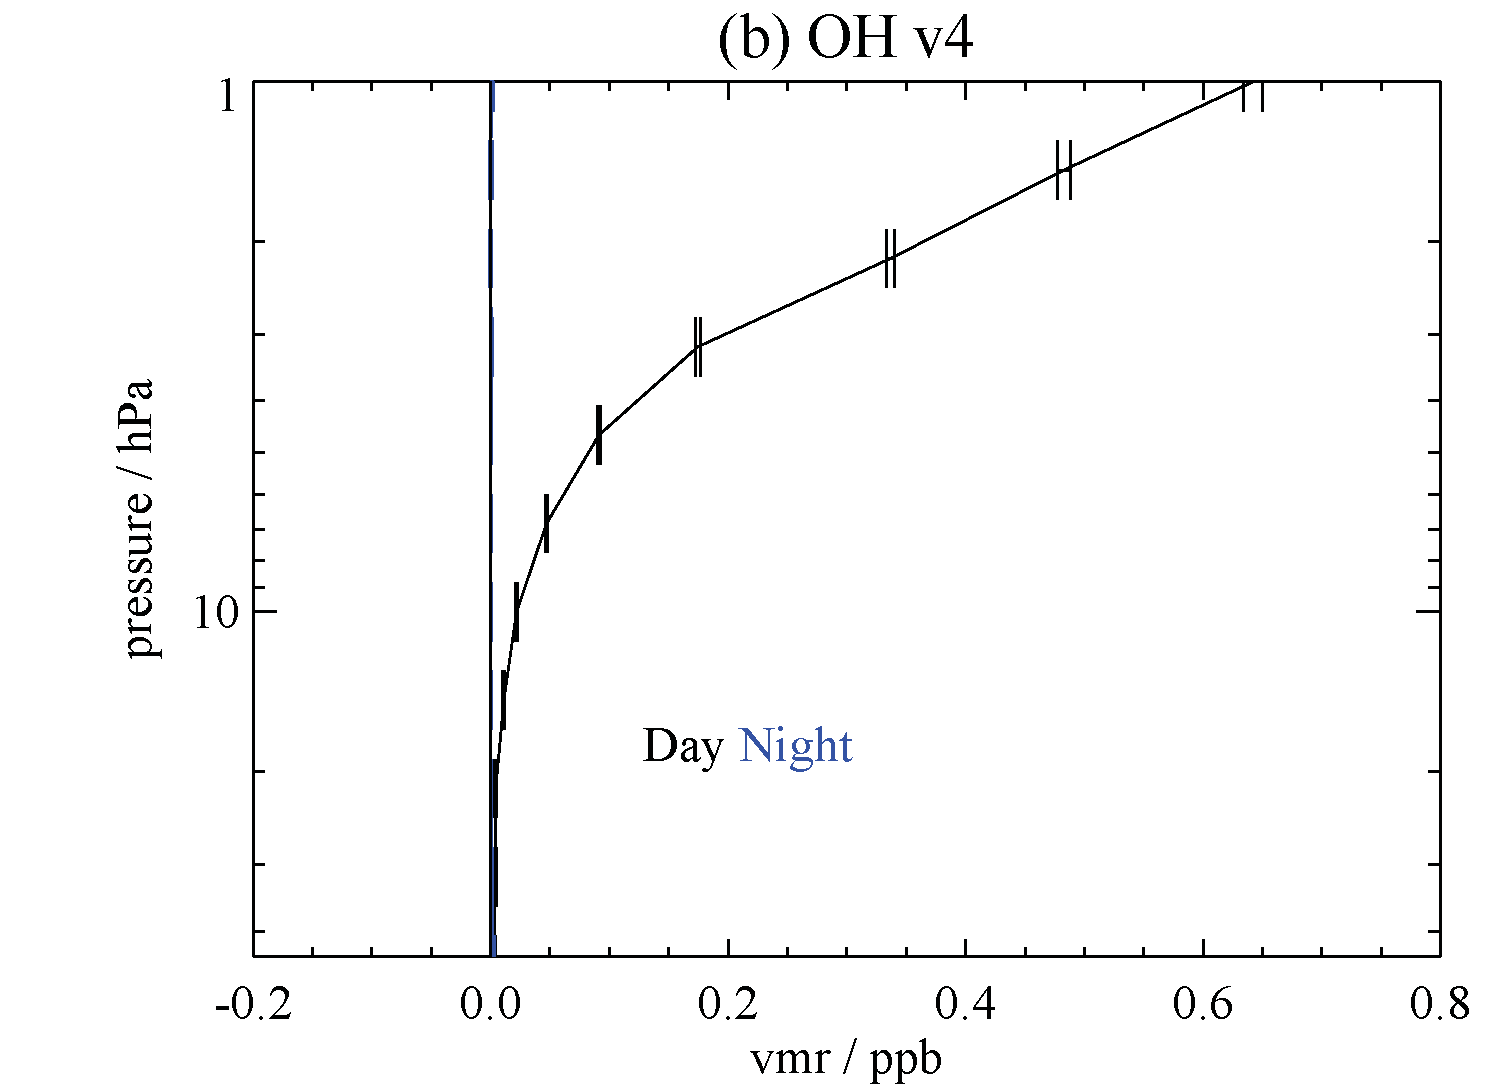
\includegraphics[width=0.5\linewidth]{figures/plot-OHv4-b}\\
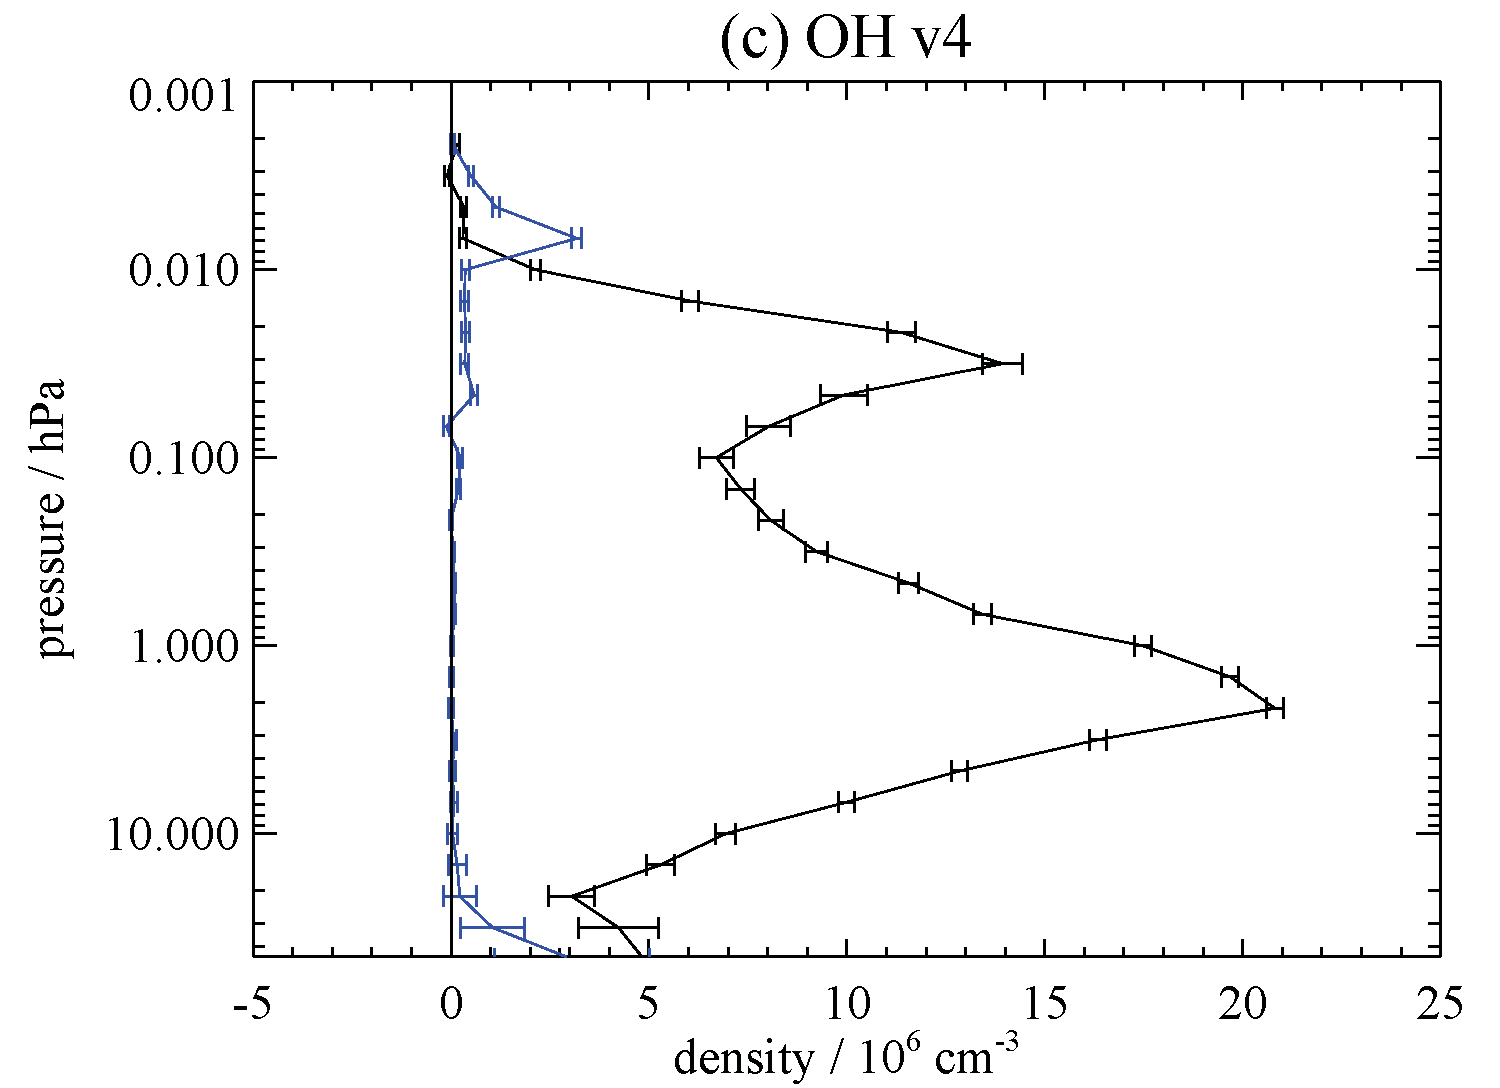
\includegraphics[width=0.5\linewidth]{figures/plot-OHv4-c}&
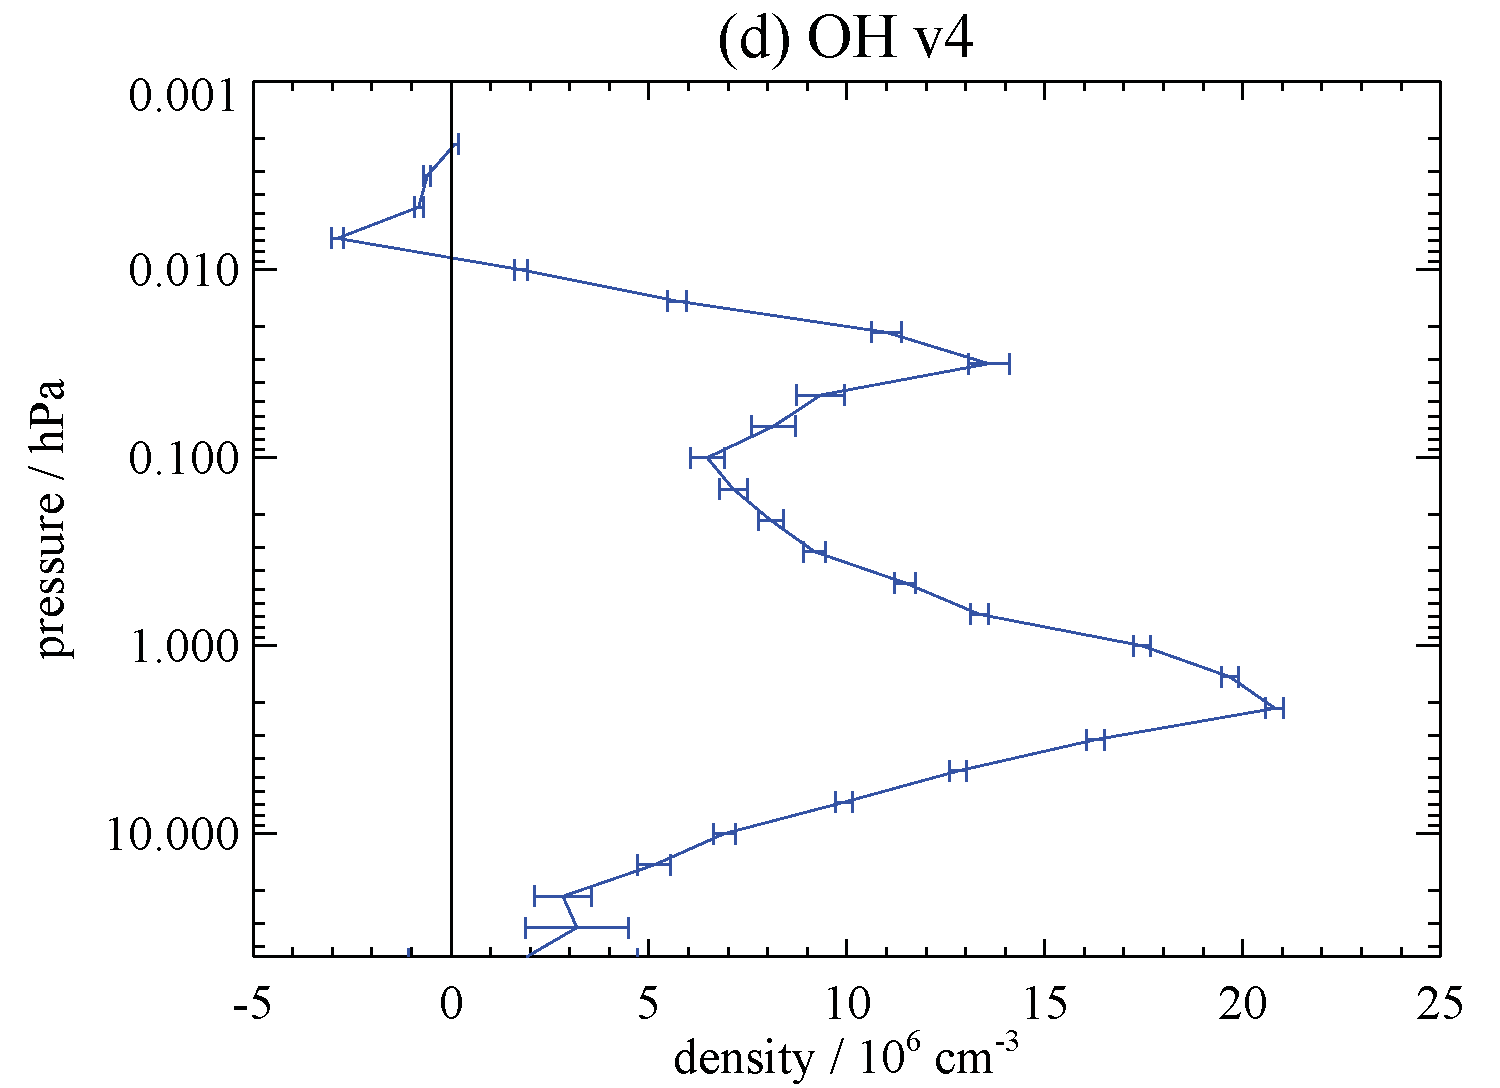
\includegraphics[width=0.5\linewidth]{figures/plot-OHv4-d}\\
\includegraphics[width=0.5\linewidth]{figures/plot-OHv3-e}&
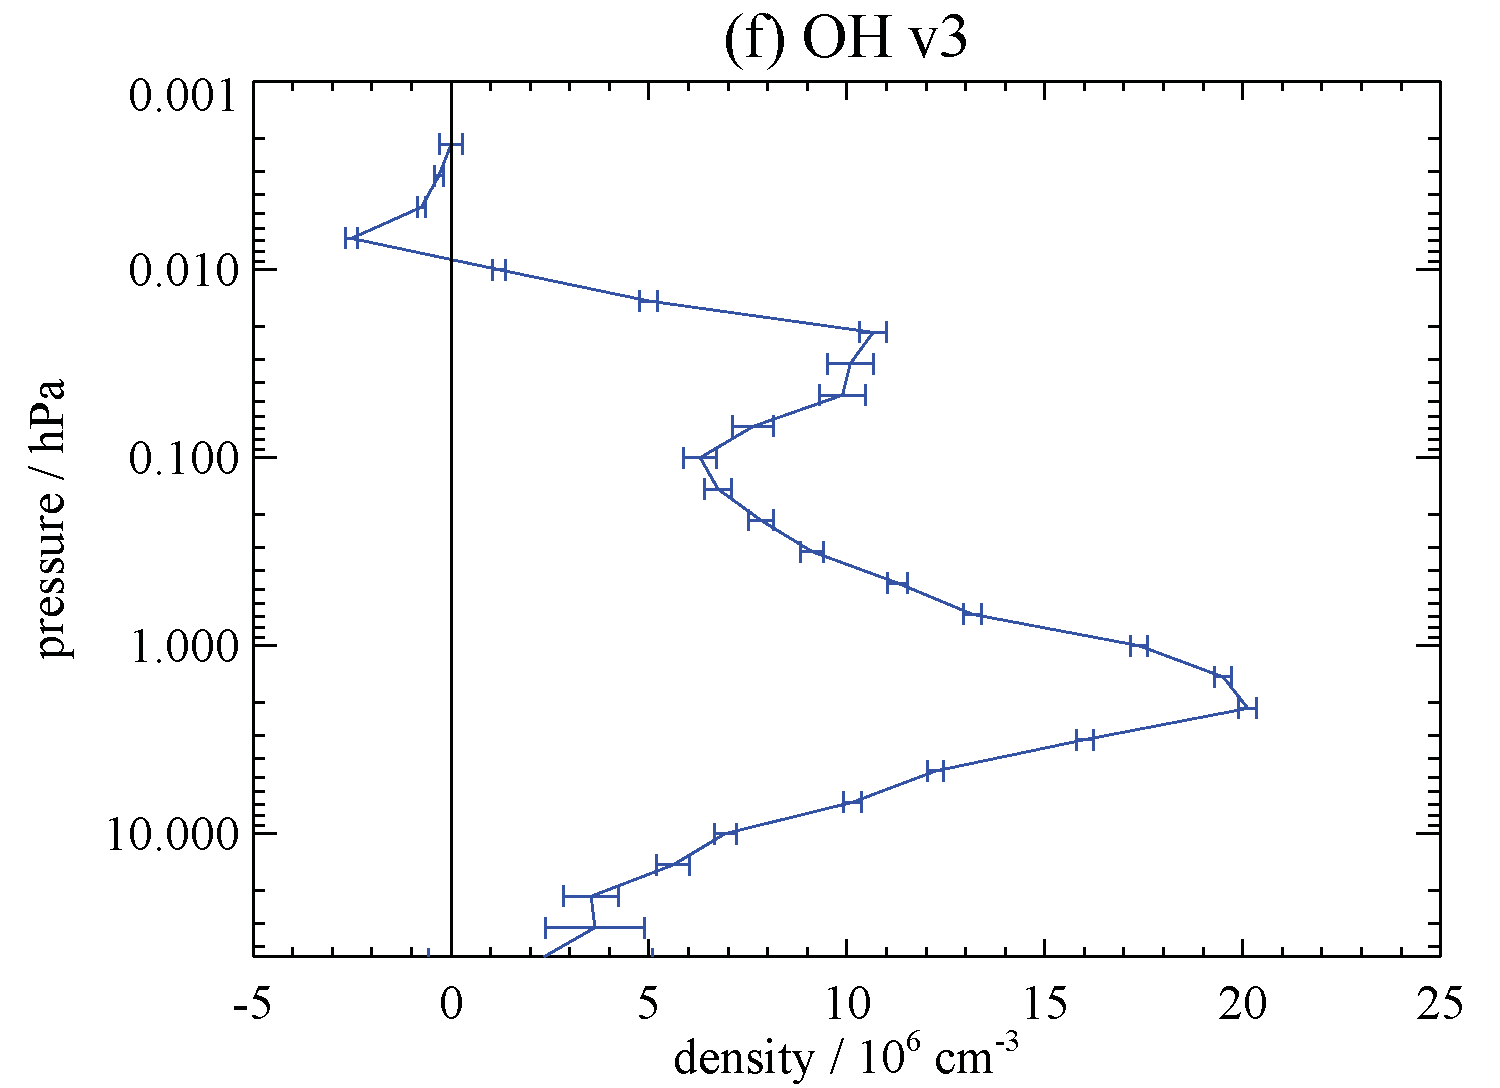
\includegraphics[width=0.5\linewidth]{figures/plot-OHv3-f}%
\end{tabular}
\caption{Zonal mean of retrieved OH and its estimated precision
  (horizontal error bars) for September 20, 2005 averaged over 29\degsym
  N to 39\degsym N\@. The average includes 98 profiles. Panel (a) shows
  \thisv OH vmr vs. pressure for day (black) and night (blue).  Panel (b)
  shows the same data plotted for the stratosphere. The retrieved night
  OH concentration is near zero for altitudes below 1\,hPa.  Panel (c)
  shows the same data in (a) converted into density units.  Panel (d)
  shows the day-night differences for the data in panel (c).  Note that
  the day-night difference is required for altitudes below 20\,hPa.
  Panels (e) and (f) are equivalent to (c) and (d) but using \prevv OH
  data.}
\label{fig:OHprofiles}
\end{figure}


\subsection*{Accuracy}

Table~\ref{tab:OHSummary} summarizes the accuracy expected for OH\@. The
scaling uncertainty is the part of the systematic uncertainty that
scales with OH concentration, e.g., spectroscopic line strength. Bias
uncertainty is the part of the uncertainty that is independent of
concentration. For both bias and scaling uncertainty, quantification of
the combined effect in MLS calibration, spectroscopy etc., on the data
product was determined by calculating the effects of each source of
uncertainty. These accuracy calculations are for \prevv products. While
no significant change is expected from \prevv to \thisv, a comprehensive
error analysis for \thisv will be conducted.  Bias uncertainty can be
eliminated by taking day-night differences from 32\,--\,21\,hPa. For
15\,--\,0.1\,hPa, the observed night OH concentration is small and
day-night differencing is not ordinarily needed. The accuracy of the OH
measurement due to systematic errors is a product of scaling uncertainty
and the observed OH concentration. The overall uncertainty is the square
root of the sum of squares of the precision and accuracy.

\subsection*{Data screening}
\label{sec:OHScreening}
It is recommended that OH data values be used in scientific
investigations if all the following tests are successful:

\begin{description}
\item[Pressure range:] \screeningrule{32\,--\,0.0032\,hPa.}
  \standardrangestatement
\standardprecisionrule
\evenstatusrule
\item[Quality:] \screeningrule{MLS \thisv HO\cs2 data can be used
    irrespective of the value of the \texttt{Quality} field.}
\item[Convergence:] \convergencerule{1.1}
\end{description}

\subsection*{Artifacts}

For some seasons, the Gas Laser Local Oscillator (GLLO) for the THz
receiver is automatically ``relocked'' as many as 5 times during a day,
leading to data gaps.  In these cases the \texttt{Status} flag is set to
\texttt{257} and the profile is ignored. This can present a problem when
compiling maps, because the missing data may appear at the same latitude
and longitude on successive days.

\subsection*{Review of comparisons with other datasets}

Data from MLS v2.2 software have been validated with two balloon-borne
remote-sensing instruments and with ground-based column measurements.
Details of the comparison are given in \citet{PickettEtal08} and
\citet{WangEtal08}.  The comparison among v2.2, \prevv, and \thisv show
no significant differences except for the mesosphere where \thisv OH
daytime values are somewhat larger and less noisy in the summer
hemisphere (or tropics when near equinox).

\begin{table}
\caption{Summary of precisions, resolution, and uncertainties for the
  MLS OH product}
\vspace{\tablecaptionsep}
\label{tab:OHSummary}
\begin{minipage}{\textwidth}\small
\centering\begin{tabular}{rccccl}
\toprule
\textbf{Pressure} &
\parbox{6em}{\bfseries\centering Resolution\\ V $\times$ H /km} &
\parbox{5em}{\bfseries\centering Precision\footnote{Precision on an
    individual profile} (day/night) / 10\cp6 cm\cp{$-$3}} &
\parbox{5em}{\bfseries\centering Bias uncertainty / 10\cp6 cm\cp{$-$3}} &
\parbox{5em}{\bfseries\centering Scaling uncertainty /\%} &
\textbf{Comments}\\
\midrule
$<$0.003\,hPa & ---                  & ---                  & ---   & --- & Unsuitable for scientific use\\
0.003\,hPa    & 5.0 $\times$ 220 & 0.5 / 0.5   & 0.034 & 90  &\\
0.01 \,hPa    & 2.5 $\times$ 180     & 1.1 /1.1             & 0.031 & 41  &\\
0.1\,hPa      & 2.5 $\times$ 165     & 3.3 / 0.6            & 0.12  & 3.1 &\\
1.0\,hPa      & 2.5 $\times$ 165     & 1.9 / 0.4            & 0.50  & 7   &\\
10 \,hPa      & 2.5 $\times$ 165     & 2.3 / 1.4            & 0.18  & 1.5 &\\
32\,--\,14\,hPa   & 2.5 $\times$ 165     & 6\,--\,10 / 4\,--\,8 & 0.50  & 1.3 & Use day--night difference \\
$>$32\,hPa & --- & --- & --- & --- & Unsuitable for scientific use\\
\bottomrule
\end{tabular}
\end{minipage}
\end{table}

%%% Local Variables:
%%% mode: latex
%%% TeX-master: "v4-x-report"
%%% End:
 \speciestitle{Relative Humidity with respect to Ice}{RHI}{RHI}{
\item[Useful range:] UTRHI, mean layer value for P $\le$ 383\,hPa,
Profile from 316\,--\,0.002\,hPa.
\item[Contact:] William Read, \email{william.g.read@jpl.nasa.gov}}

\subsection*{Introduction}

RHi is relative humidity with respect to ice. The vertical grid for RHi
is 12 levels per decade change in pressure for 1000\,--\,1.0 hPa
thinning to 6 levels per decade for 1.0\,--\,0.1\,hPa and finally 3
levels per decade for 0.1\,--\,10\cp{$-$5}\,hPa.  The RHi product is a
fusion of information from two separate retrievals.  From
1000\,--\,383\,hPa, RHi is retrieved directly from optically thick
radiances using measurement and retrieval principles similar to nadir
sounding humidity receivers (e.g., TOVS).  All grid levels between
1000\,--\,383\,hPa are filled with a uniform ``UTRHI'' (upper
tropospheric relative humidity with respect to ice) value representing
the mean value of a broad layer (\texttildelow4\,--\,6\,km) that peaks
between \texttildelow350\,hPa (in the moist tropics) and
\texttildelow650\,hPa (typical for dry high latitudes).  This humidity
is used as a lower altitude constraint and \emph{a priori} for the
vertically resolved humidity product that begins at 316\,hPa. From
316\,--\,0.002\,hPa, RHi is derived from the standard products of water
and temperature using the Goff-Gratch ice humidity saturation
formula. RHi validation is presented in
\citet{ReadEtal07}. Table~\ref{tab:RHISummary} is summary of precision,
resolution, and accuracy.

\subsection*{Changes from v3}

The main differences between v4.2 and v3.3 relate to cloud screening and
improvements in the \texttt{InitUTH} initial upper tropospheric and
lower stratospheric humidity estimation phase that produces the first
guess and sets smoothing constraints on the H\cs2O profile retrieved in
the final retrieval phase that produces the standard product. There have
been no spectroscopy changes either in linewidth or continuum
charaterization between v4 and v3. An improved cloud detection
methodology has been developed for v4 that does a better job of
rejecting cloudy radiances that are likely to cause poor fits and
corrupted profiles. The number of erroneous spikes in the upper
troposphere has been reduced in v4 relative to v3. The \texttt{InitUTH}
phase retrieves H\cs2O on a more coarse 6 levels per decade grid. The
\texttt{InitUTH} H\cs2O is used for the initial guess for the final
12~levels per decade retrieval and sets smoothing constraints for the
profile shape instead of smoothing to the shape of a climatological
\emph{a priori} profile.  The \texttt{InitUTH} phase has been expanded to use
more channels and better forward model representations to improve its
retrieval accuracy. In addition, the retrieval range has been expanded
to have its top moved from 100\,hPa (in v3) to 10\,hPa (in v4). This
change makes a more seamless transition from the troposphere to the
stratosphere. Simulation studies show that these changes have improved
the agreement between the ``truth'' profiles used to produce the
simulated radiances and the retrieved profiles in the 316\,--\,215\,hPa
levels.

\begin{figure}
\begin{center}
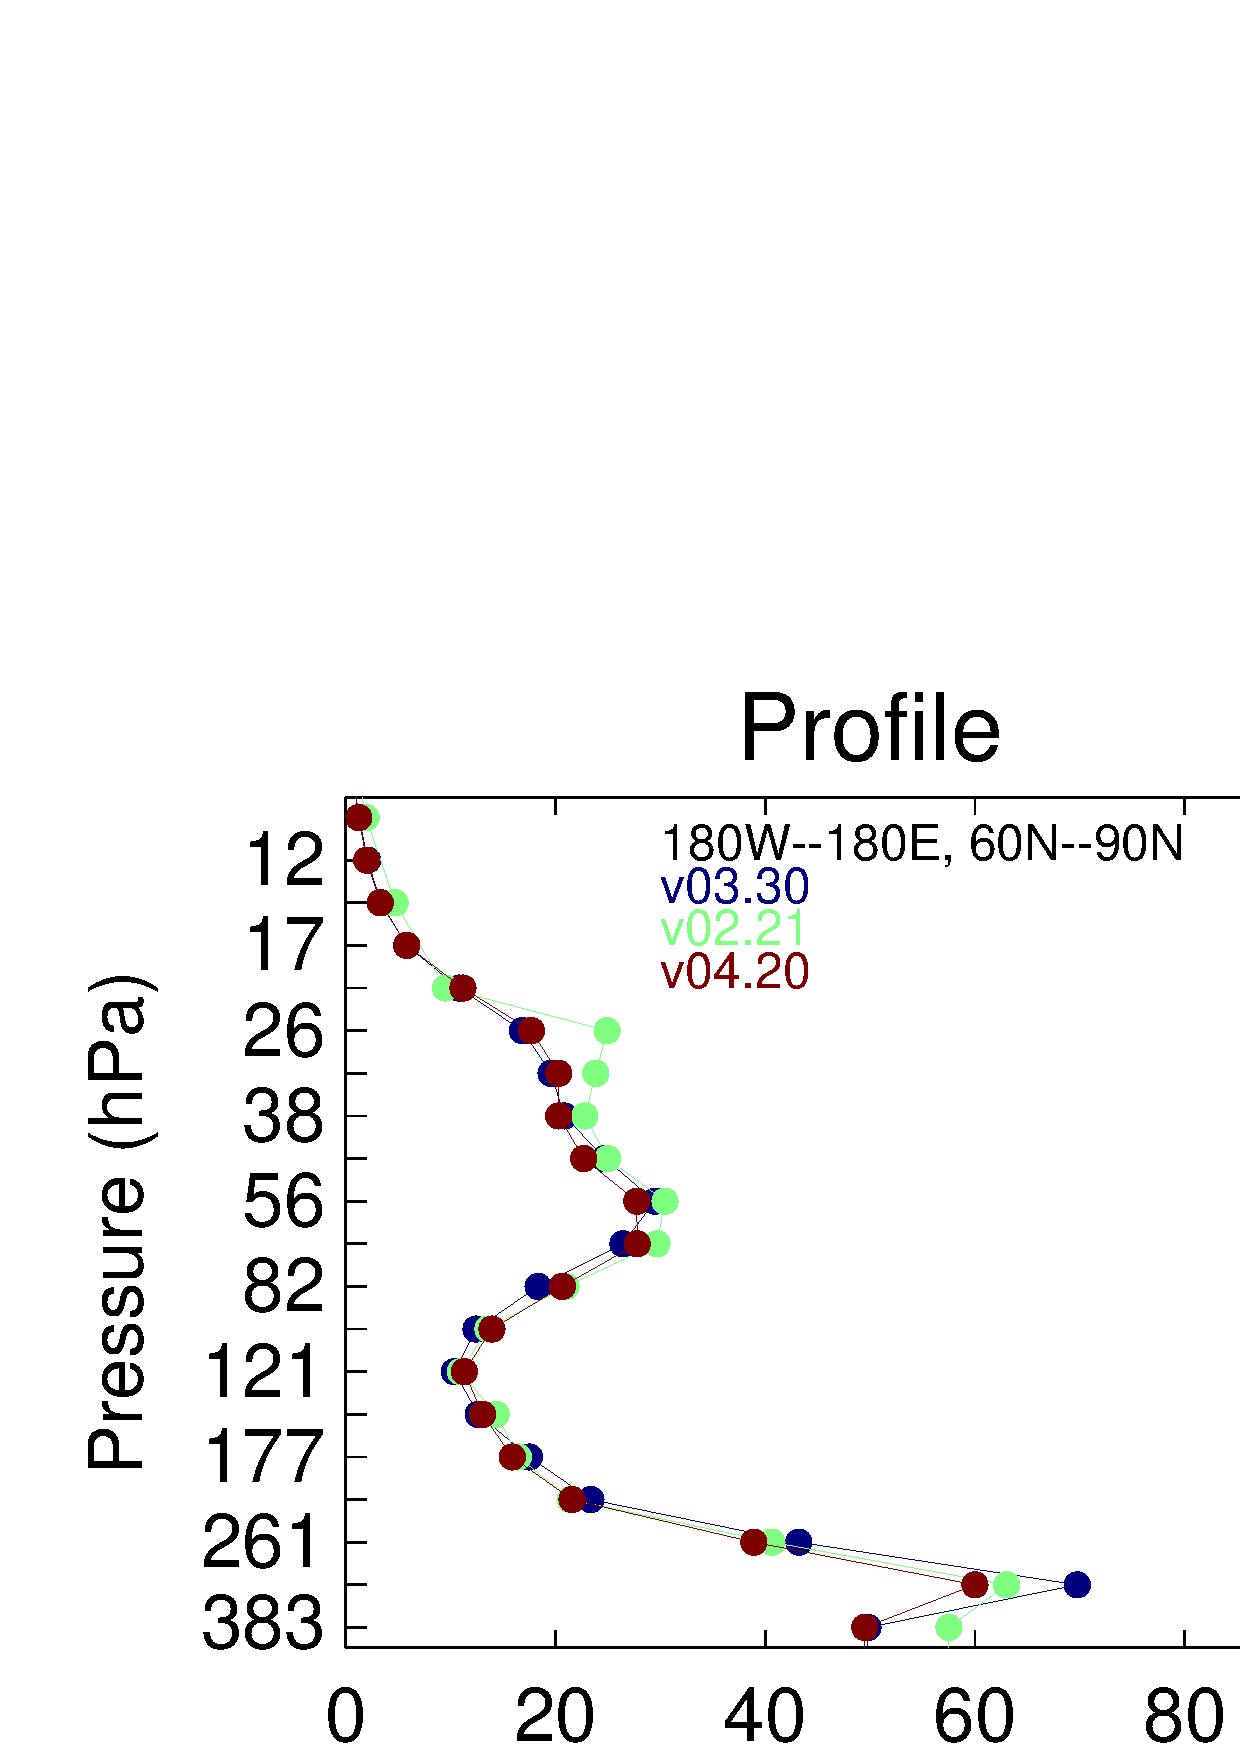
\includegraphics[width=0.8\linewidth]{figures/mls_rhi_v3-v4_prfl_comp_60n-90n}
\includegraphics[width=0.8\linewidth]{figures/mls_rhi_v3-v4_prfl_comp_30n-60n}
\includegraphics[width=0.8\linewidth]{figures/mls_rhi_v3-v4_prfl_comp_30s-30n}
\includegraphics[width=0.8\linewidth]{figures/mls_rhi_v3-v4_prfl_comp_60s-30s}
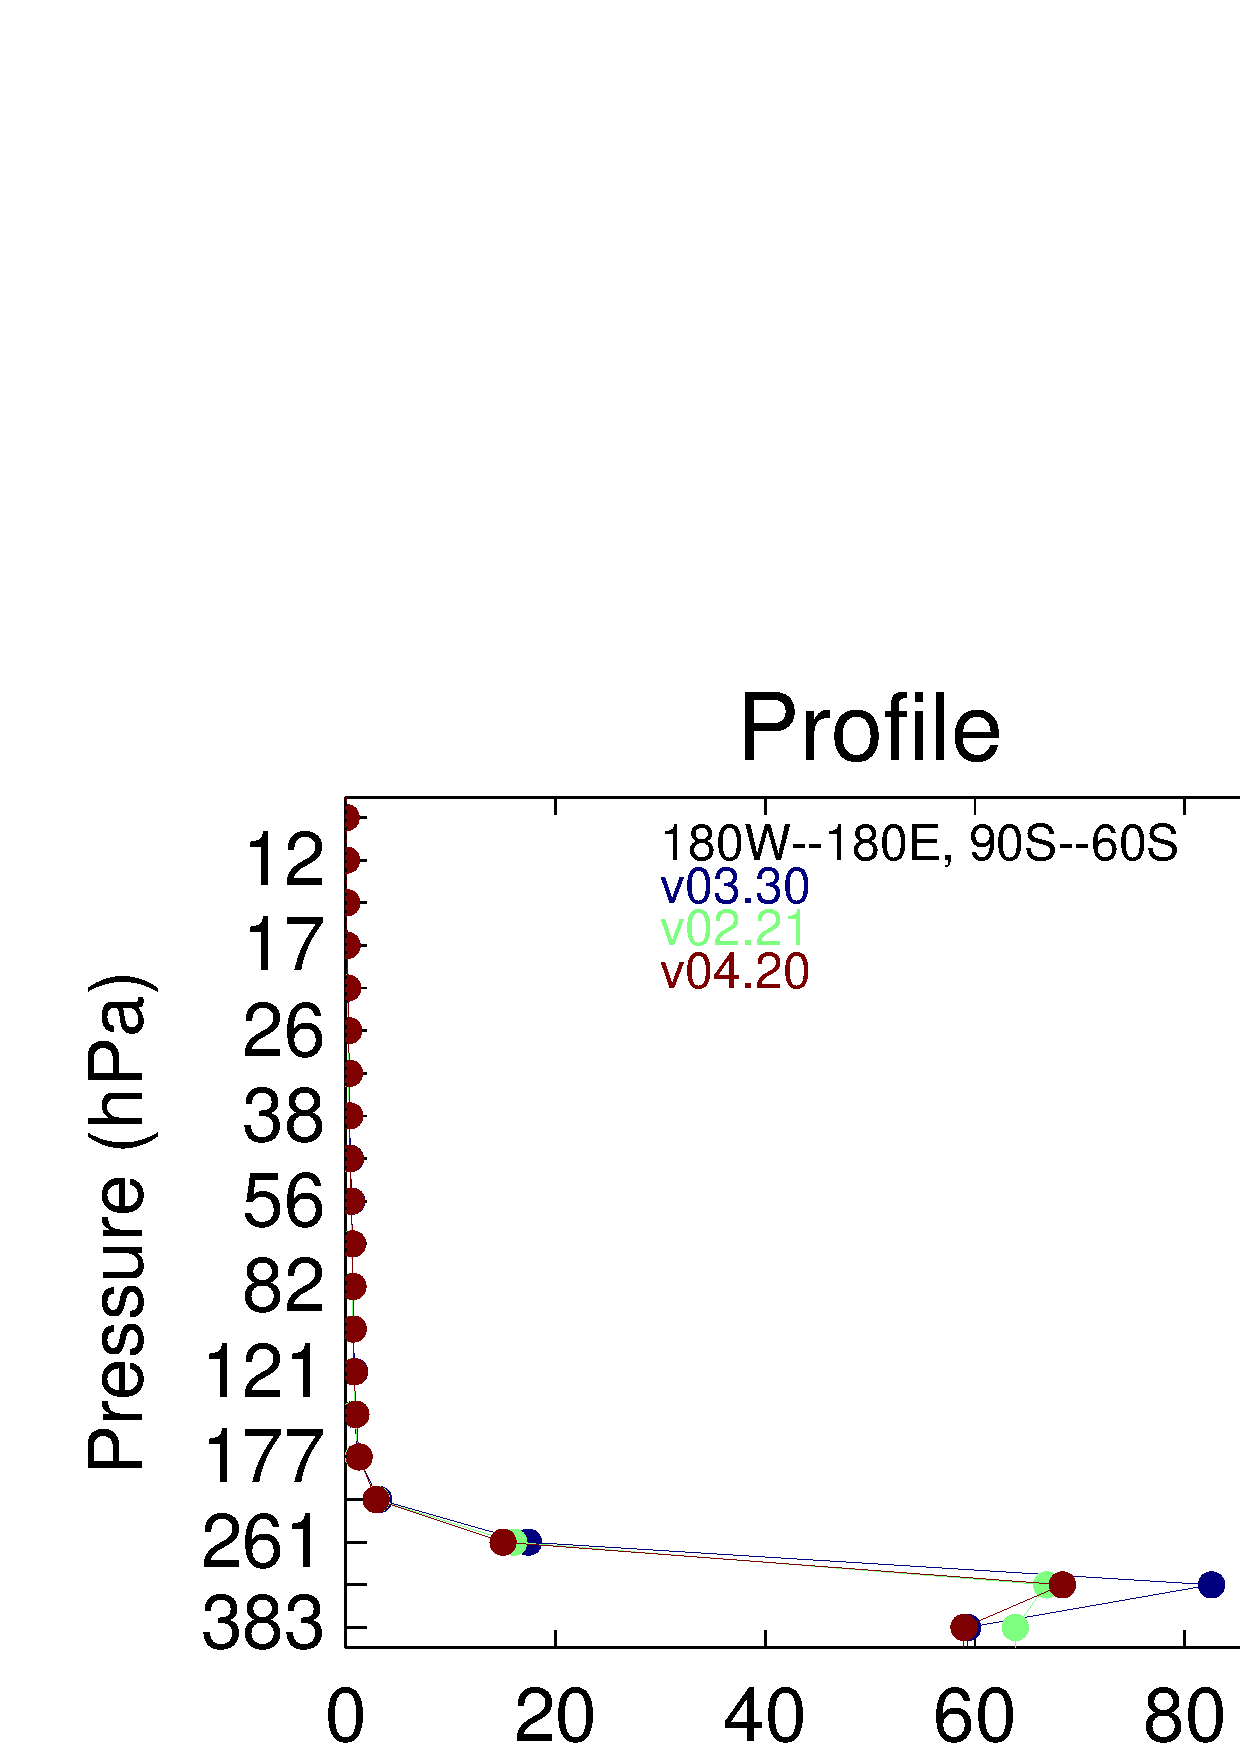
\includegraphics[width=0.8\linewidth]{figures/mls_rhi_v3-v4_prfl_comp_90s-60s}
\end{center}
\caption{A comparison of
  v3.3 (blue), v2.2(green), and v4.2 (red) rhi for Jan-Feb-Mar 2005 in 5
  latitude bands. Other time periods are similar. The left panel
  compares mean profiles, the center shows the mean difference (red and green
  diamonds) surrounded by each versions' estimated precision, and the
  right panel shows the estimated retrieval precision (solid and
  bullets) and measured variability (dotted) which includes atmospheric
  variability about the mean profile.}
\label{fig:avgmlsrhiprflcomp}
\end{figure}

Figure~\ref{fig:avgmlsrhiprflcomp} compares MLS v4.2 to v3.3. RHI shows
bigger differences than that for H\cs2O because it also includes changes
between the two versions for temperature. The differences sometimes
exceed 20\% and can be either a low or high bias.

Relative humidity data at pressures greater than 316\,hPa are derived
from a broad layer relative humidity retrieval (using low limb viewing
MLS wing channel radiances) similar to that obtained from NOAA
operational humidity sounders such as TOVS\@. As noted in
\citep{ReadEtal07}, the v2.2 retrieval at these pressures was likely to
be \texttildelow30\% too high based on comparisons with AIRS\@.  The
accuracy of this retrieval is highly sensitive to the transmission
efficiency of the MLS optics system. In v3.3 this was adjusted
empirically (within the uncertainty range established from MLS
calibration) to give better agreement with AIRS in the tropics. In v4
the N\cs2 continuum was adjusted only for this phase to minimize the
clear sky cloud induced radiance bias.  This retrieval is used as an a
priori and profile constraint for the humidity profile at pressures
greater than 316\,hPa which are not retrieved in the standard H\cs2O
product retrieval.

The third panel in Figure~\ref{fig:avgmlsrhiprflcomp} shows the mean
estimated single profile precision and the measured variability (which
includes instrument noise and atmospheric variability). The precisions
for the two versions are nearly identical except for pressures greater
than 68\,hPa, where v4 produces lower values.

\subsection*{Resolution}

RHi for pressures of 316\,hPa and smaller is a derived product and
therefore a retrieval averaging kernel is not directly available.  An
estimate for the spatial resolution (vertical X along track) of this
product is a convolution of the temperature and H\cs2O
resolutions. Since temperature has lower spatial resolution than H\cs2O
in the troposphere and lower stratosphere it is assumed that the spatial
resolution of temperature shown in Figure~\ref{fig:AvkTemperature_HR}
best represents the resolution of the RHi product. The cross track
resolution is probably 12\,km, the larger of temperature and H\cs2O
cross track resolutions.  These resolutions are only true in the limit
that the mean $\log$( H\cs2O) doesn't change appreciably over the
broader temperature measurement volume. The longitudinal separation of
the MLS measurements, set by the Aura orbit, is 10\degsym--\,20\degsym\
over middle and lower latitudes, with much finer sampling in polar
regions.

The RHi for pressures greater than 316\,hPa, represents a mean value in
a broad layer (4\,--\,6\,km) whose sensitivity peaks between
\texttildelow350\,hPa (in the moist tropics) and \texttildelow650\,hPa
(typical for dry high latitudes).

\subsection*{Precision}

The values for precision are the root sum square (RSS) precisions for
H\cs2O and temperature propagated through the Goff-Gratch relationship,
see sections~\ref{navSectionH2O} and~\ref{navSectionTemperature} for
more details. The precisions are set to negative values (or zero in some
cases) in situations when the retrieved precision is larger than 50\% of
the a priori precision for either temperature or H\cs2O --- an
indication that the data is biased toward the a priori value.

\subsection*{Accuracy}

The values for accuracy are the RSS accuracies for H\cs2O and
temperature scaled into \%\,RHi units. see
sections~\ref{sec:StandardH2O} and~\ref{sec:StandardTemperature} for
more details.  These may change for the v4 RHi product. The MLS team
plans to repeat the v3 exercise with the v4 software and release the
results in a subsequent version of this document.

\subsection*{Data screening}
\label{sec:RHIScreening}
\begin{description}

\item[Pressure range:] \screeningrule{Profile from 316\,--\,0.002\,hPa,
    larger pressures represent mid/upper troposphere column.}
  \standardrangestatement \standardprecisionrule \evenstatusrule

\item[Clouds:] Ignore status bits 16 (high clouds) or 32 (low clouds)
  set indicating the presence of clouds. See artifacts for more details.

\item[Quality field:] \screeningrule{The \texttt{Quality} fields for
    both the \texttt{L2GP-RHI} and \texttt{L2GP-Temperature} swaths need
    to be considered, as described below:}
  \begin{description}
  \item[For pressures of 83\,hPa and smaller:] Use only profiles with
    RHi \texttt{Quality} \emph{greater} than 1.45 and Temperature
    \texttt{Quality} \emph{greater} than 0.2
  \item[For pressures of 100\,hPa and larger:] Use only profiles with
    RHi \texttt{Quality} \emph{greater} than 1.45 and Temperature
    \texttt{Quality} \emph{greater} than 0.9.
  \end{description}

\item[Convergence field:] \screeningrule{Only profiles with a value of
    the RHi \texttt{Convergence} \emph{less} than 2.0 and Temperature
    \texttt{Convergence} \emph{less} than 1.03 should be
    used in scientific studies.}

\item[Temperature precision:] The \texttt{L2gpPrecision} field in the
  \texttt{L2GP-Temperature} file can be used to further eliminate
  outliers that are believed to be the result of thick clouds, primarily
  in the tropics.  If careful screening of the troposphere is required,
  levels 261\,--\,178\,hPa should be avoided if any of the following
  criteria are met:
\begin{description}
\item[At 316\,hPa:] \texttt{L2gpPrecision} $>1.1$\,K \textbf{and} latitude $> -60\degsym$
\item[At 261\,hPa:] \texttt{L2gpPrecision} $>0.7$\,K 
\item[At 215\,hPa:] \texttt{L2gpPrecision} $>0.825$\,K 
\end{description}

\item[End of day (v4.20 only):] The last four profiles of each day show
  greatly increased rates of large temperature departure from \emph{a
    priori}.  Accordingly the last four profiles of the RHI product each
  day should not be used in v4.20.  The issue is fixed in v4.22.
\end{description}

\subsection*{Artifacts}

See sections~\ref{sec:StandardH2O} for H\cs2O
and~\ref{sec:StandardTemperature} for temperature for specific issues
related to these parent products. Effects of MLS temperature precision
(\texttildelow1\,--\,2\,K) must be considered if one wishes to use MLS
RHi to study supersaturation. In simulation studies, systematic errors
(such as tangent pressure retrieval and errors), in addition to
introducing biases, also increase variability in differences with
respect to a ``truth'' data set particularly for pressures greater than
200\,hPa. This will add to the frequency of supersaturation in the tail
of MLS RHi distribution functions.  Therefore, MLS RHI is not
recommended for studying statistics of supersaturation at pressures
greater than 178\,hPa. For smaller pressures, one must remove the
contribution from temperature noise as part of the analysis.
Measurements taken in the presence of clouds significantly degrade the
precision, that is increases the scatter about the mean, but the mean
bias as compared to AIRS changes by less than 10\%.

The last four temperature profiles of each day show increased rates of
outliers relative to GEOS-5 temperature, compared to other profile
positions in the day.  These outliers can be as large as 50\,K at some
levels.  Attempts to address this end of day boundary problem by
creating daily overlap periods that can be discarded have not yet
satisfactorily addressed this problem and the magnitude of the outliers
has increased somewhat in \thisv.  A recommendation to discard the last
4 profiles of each day for temperature, GPH, and RHI has been added to
recommended screening.


\subsection*{Review of comparisons with other datasets}

Figures~\ref{fig:rhiairsmlsjf2005maps} and
\ref{fig:rhiairsmlsjja2005maps} show comparisons between AIRS v6 and MLS
v2, 3, and 4. Mapped features tend to agree well but MLS produces higher
relative humidities in the moist regions of the tropics relative to
AIRS. Version 4 at 300\,hPa in high northern latitudes during January
and February show marked improvement over the earlier versions by
comparison to AIRS\@. Except as noted previously, the three MLS versions
show little change amongst themselves.

\begin{figure}
\begin{center}
  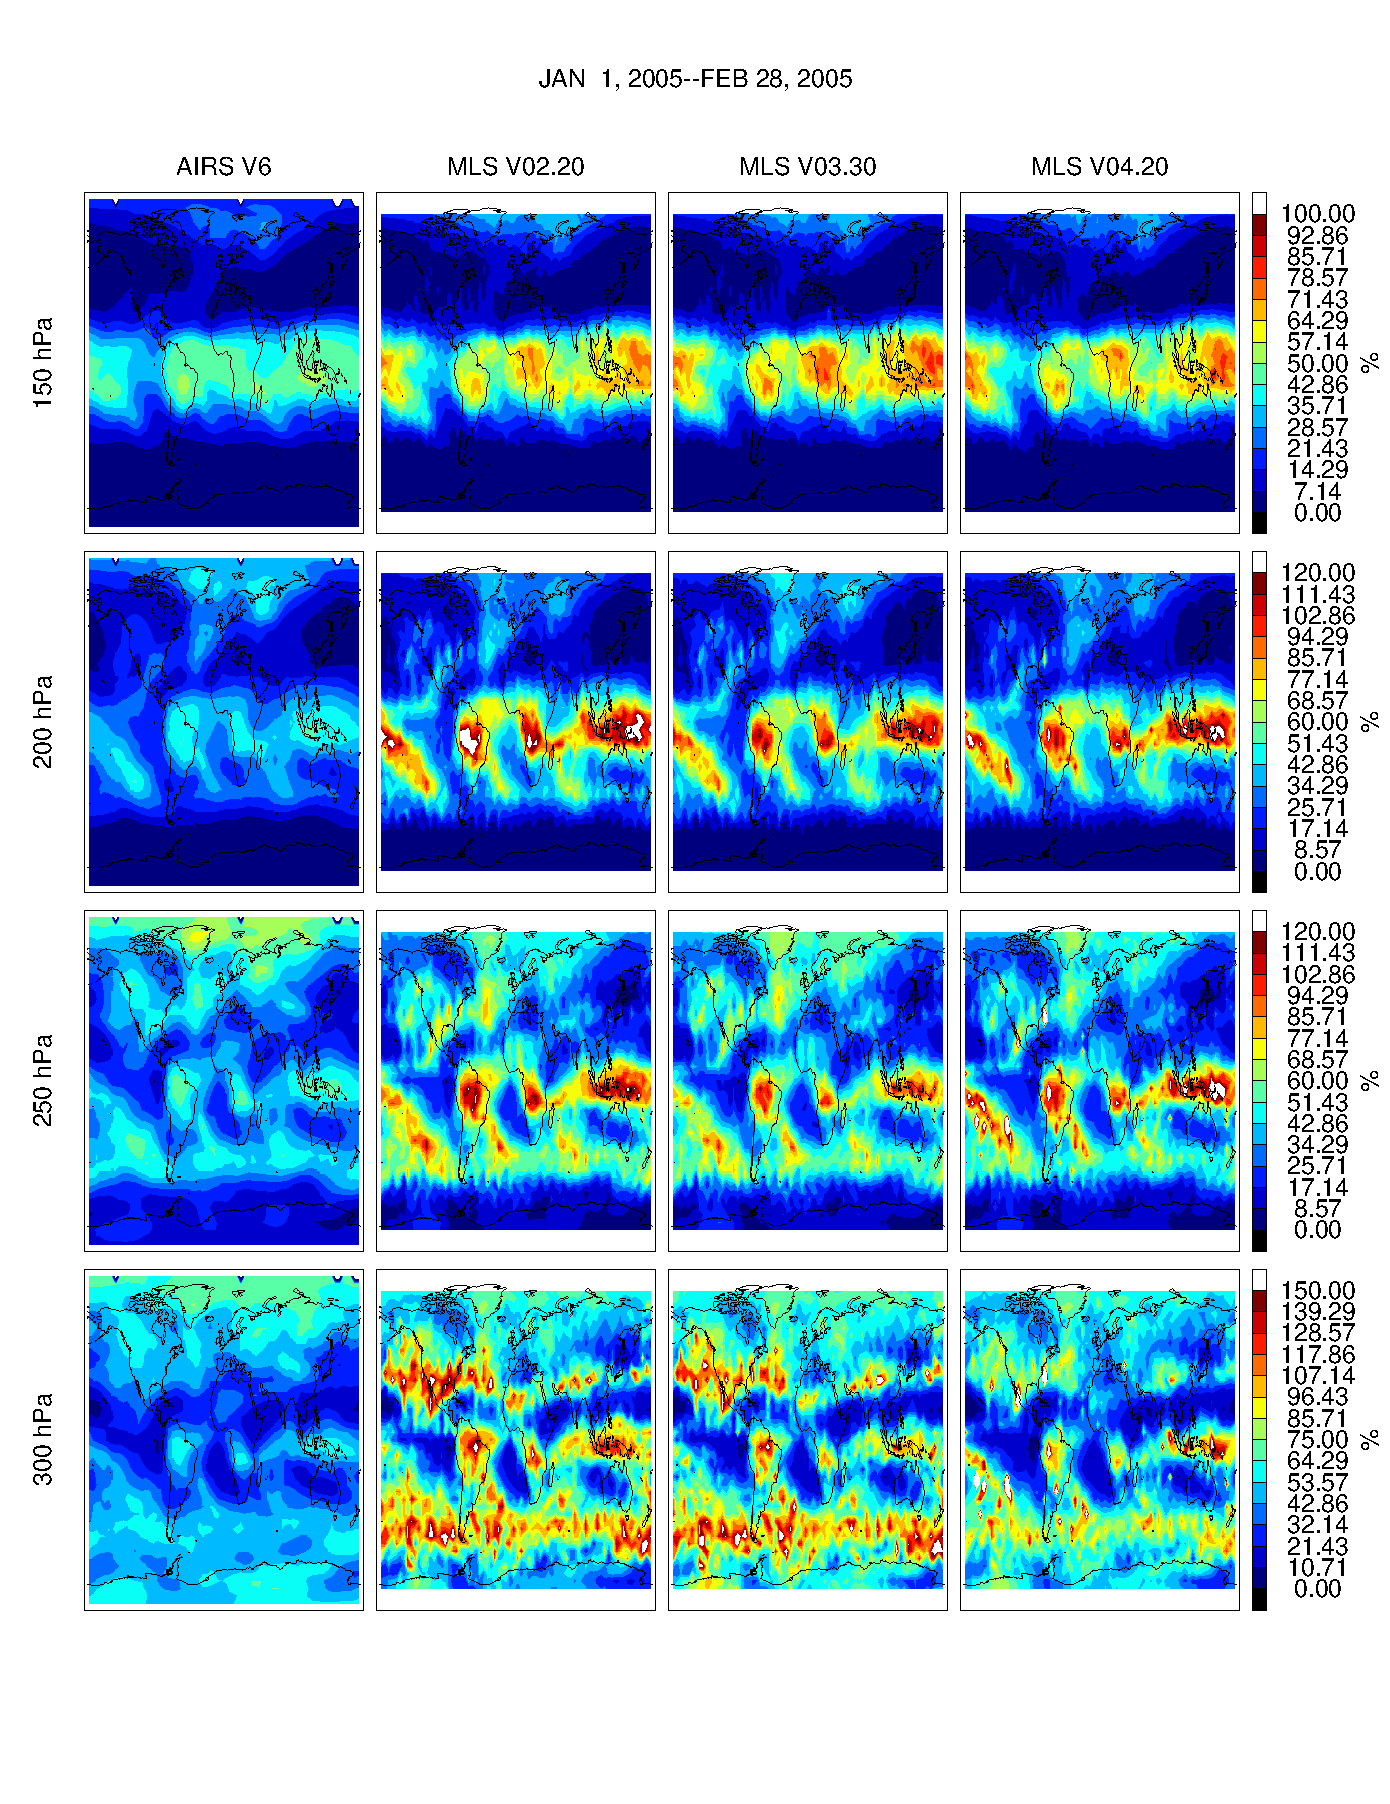
\includegraphics[width=0.9\linewidth]
{figures/rhi_grid_maps_jf2005_airsv6-mlsv3andv4}
\end{center}
\caption{Mapped fields from AIRS v6 (left), MLS v2.2 (center-left), MLS v3.3
(center-right), and MLS v4.2 (right) pressures between 300--150 hPa for
January and February 2005.}
\label{fig:rhiairsmlsjf2005maps}
\end{figure}

\begin{figure}
\begin{center}
  \includegraphics[width=0.9\linewidth]
{figures/rhi_grid_maps_jja2005_airsv6-mlsv3andv4}
\end{center}
\caption{Mapped fields from AIRS v6 (left), MLS v2.2 (center-left), MLS v3.3
(center-right), and MLS v4.2 (right) pressures between 300--150 hPa for
June--August 2005.}
\label{fig:rhiairsmlsjja2005maps}
\end{figure}


\subsection*{Desired improvements}

We are aiming to improve high latitude performance of 261 and 215\,hPa
H\cs2O in future work.

\begin{table}
\caption{Summary of MLS v3.3 UTLS RHi product.}
\vspace{\tablecaptionsep}
\label{tab:RHISummary}
\begin{minipage}{\linewidth}
\centering\begin{tabular}{ccccl}
\toprule
\parbox[m]{5em}{\bfseries\centering Pressure / hPa} &
\parbox[m]{5em}{\bfseries\centering Resolution V~$\times$~H \ km} &
\parbox[m]{7em}{\bfseries\centering Single profile precision
\footnote{Absolute error in percent} / \%} &
\parbox[m]{6em}{\bfseries\centering Accuracy%
  \footnote{Fractional error ( [error in RHi] / RHi) in percent}/ \%} &
\bfseries Comments
\\ \midrule
0.001  & --- & ---  & --- & Unsuitable for scientific use \\  
0.002 &13 $\times$ 230 & 190  &100 &  \\
0.004 &13 $\times$ 260 & 100  &100 & \\
0.010 &12 $\times$ 590 & 50   &100 & \\
0.022 &12 $\times$ 750 & 40   &100 & \\
0.046 &16 $\times$ 400 & 30   &100 & \\
0.10  &14 $\times$ 420 & 30   &100 & \\
0.22  & 8 $\times$ 370 & 20   & 90 & \\
0.46  & 8 $\times$ 320 & 15   & 75 & \\
1.00  & 8 $\times$ 280 & 15   & 60 & \\
2.15  & 8 $\times$ 250 & 15   & 35 & \\
4.64  & 6 $\times$ 220 & 15   & 15 & \\
10& 4 $\times$ 210 & 15   & 15 & \\ 
22& 4 $\times$ 210 & 15   & 20 & \\
46& 4 $\times$ 210 & 15   & 25 & \\
68& 4 $\times$ 200 & 15   & 25 & \\
83& 4 $\times$ 200 & 20   & 25 & \\
100& 4 $\times$ 200 & 20   & 20 & \\
121& 4 $\times$ 200 & 25   & 20 & \\
147& 4 $\times$ 200 & 25   & 20 & \\
178& 4 $\times$ 200 & 35   & 30 & \\
215& 4 $\times$ 200 & 45   & 35 & see Table~\ref{tab:H2OSummary} \\
261& 4 $\times$ 200 & 45   & 30 & see Table~\ref{tab:H2OSummary} \\
316& 6 $\times$ 200 & 70   & 20 & see Table~\ref{tab:H2OSummary} \\
UTRHI, $>$316 & 6 $\times$ 150 & 40(est) & 10(est) & measurement height
depends \\
&                &    &     &   on atmospheric humidity \\
\bottomrule
\end{tabular}
\end{minipage}
\end{table}

%%% Local Variables: 
%%% mode: latex
%%% TeX-master: "v4-x-report"
%%% End: 
 \speciestitle{Sulfur Dioxide}{SO\cs2}{SO2}{%
\item[Useful range:] 215\,--\,10.0\,hPa
\item[Contact:] William Read, \email{william.g.read@jpl.nasa.gov}}

\subsection*{Introduction}

The standard SO\cs2 product is taken from the 240-GHz retrieval
(\texttt{CorePlusR3}). MLS can only measure significantly enhanced
concentrations above nominal background such as that from volcanic
injections. Validation of SO\cs2 is published in \citet{PumphreyEtal14}.

\subsection*{Changes from v3}

The v4 SO\cs2 retrieval has two significant changes from v3. The first is a
different method of modeling the background radiance signal from unknown
or unaccountable sources. The method is specifically designed to be more
immune to clouds. The other change is an improved cloud detection and radiance
rejection algorithm. These changes have significantly improved the
convergence and quality performance of the retrieval system and
eliminated much of the poor in-cloud behavior present in v3. There have
been no changes to the spectroscopic characteriztion of the major
species in the 240~GHz bands used to retrieve SO\cs2.

\begin{figure}
\begin{center}
\includegraphics[clip, width=0.8\linewidth]{figures/mls_so2_v3-v4_prfl_comp_60n-90n}
\includegraphics[clip, width=0.8\linewidth]{figures/mls_so2_v3-v4_prfl_comp_30n-60n}
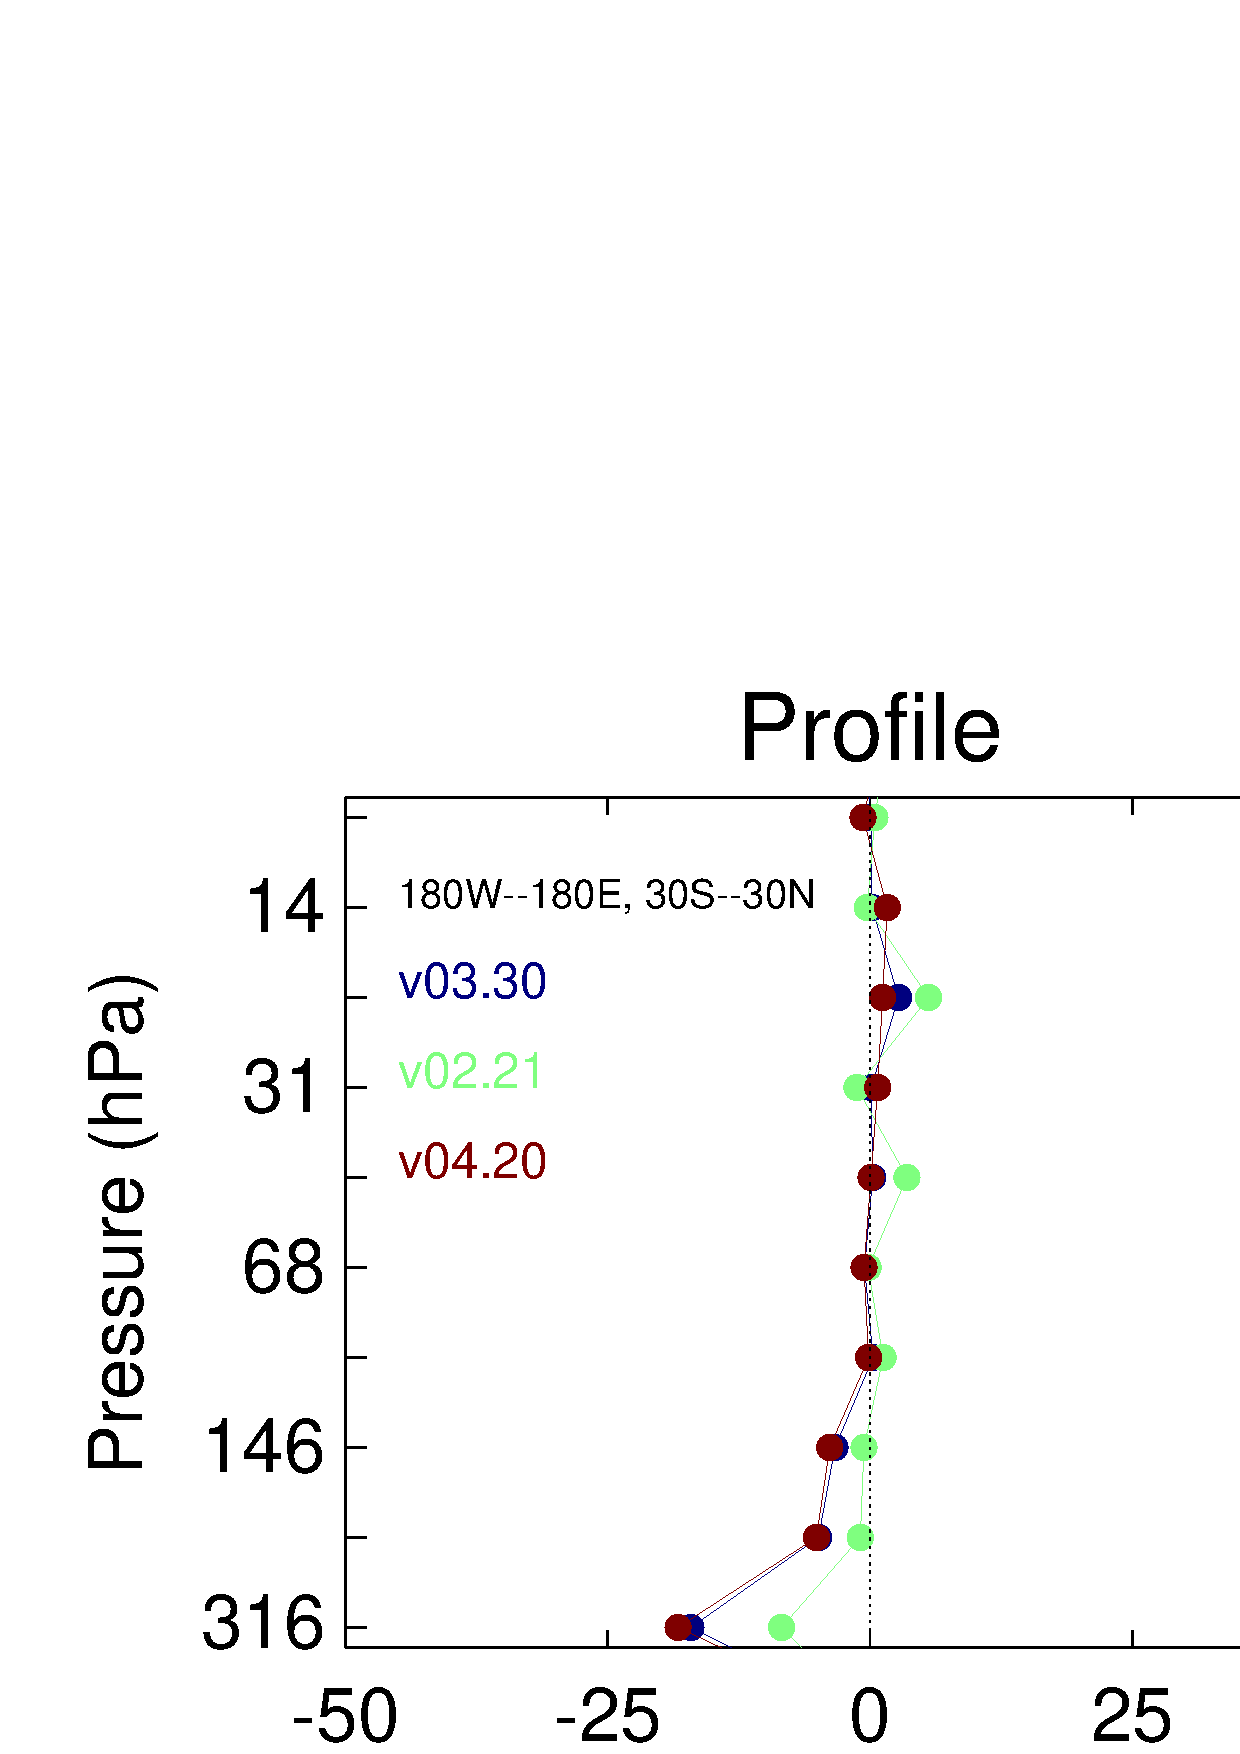
\includegraphics[clip, width=0.8\linewidth]{figures/mls_so2_v3-v4_prfl_comp_30s-30n}
\includegraphics[clip, width=0.8\linewidth]{figures/mls_so2_v3-v4_prfl_comp_60s-30s}
\includegraphics[clip, width=0.8\linewidth]{figures/mls_so2_v3-v4_prfl_comp_90s-60s}
\end{center}
\caption{A comparison of
  v3.3 (blue) and v4.2 (red) SO\cs2 for Jan-Feb-Mar 2005
  in 5 latitude bands. Other time periods are similar. The left panel
  compares mean profiles, the center shows the mean difference (red
  diamonds) surrounded by each versions' estimated precision, and the
  right panel shows the estimated retrieval precision (solid and
  bullets) and measured variability (dotted) which includes atmospheric
  variability about the mean profile.}
\label{fig:avgmlsso2prflcomp}
\end{figure}

Figure~\ref{fig:avgmlsso2prflcomp} compares MLS v4.2 and v3.3. The
atmosphere typically has \texttildelow0.1\,ppbv SO\cs2, which is far
smaller than the MLS SO\cs2 accuracy estimate.  Both versions
(erroneously) report typical abundance of order of a few ppbv, due to
systematic errors in the MLS measurement system. The $-20\,\text{ppbv}$
reported at 215\,hPa is also a systematic artifact.

\subsection*{Resolution}
\onestandardavk{SO2}{SO\cs2}%

Based on Figure~\ref{fig:AvkSO2}, the vertical resolution for SO\cs2 is
\texttildelow3\,km and the horizontal resolution is 170\,km. The
horizontal resolution perpendicular to the orbit track is 6\,km, the
full width at half maximum of the MLS antenna, for all pressures.

\subsection*{Precision}

The estimated precision for SO\cs2 is \texttildelow4\,ppbv for all
heights between 215\,--\,10\,hPa. The precisions are set to negative
values (or zero in some cases) in situations when the retrieved
precision is larger than 50\% of the a priori precision -- an indication
that the data is biased toward the a priori value.

\subsection*{Accuracy}

The values for accuracy are based on the v3 systematic error analysis
performed on the MLS measurement system \citep{ReadEtal07}. The accuracy
is estimated to be \texttildelow5\,ppbv for pressures less than 147\,hPa
increasing to \texttildelow20\,ppbv at 215\,hPa. These may be different
for the v4 SO\cs2 product. The MLS team plans to repeat the v3 exercise
with the v4 software and release the results in a subsequent version of
this document.

\subsection*{Data screening}
\label{sec:SO2Screening}
\begin{description}
\item[Pressure range:] \screeningrule{215\,--\,10.0\,hPa} \standardrangestatement
\item[Estimated Precision:] \screeningrule{Values with negative
    precision can be used, though with caution.}

  Although it is generally recommended to not use values where precision
  is flagged negative, SO\cs2 is an exception and it is appropriate to
  use values with negatively flagged precision (provided that the entire
  profile is not so flagged). High retrieved values of SO\cs2 at the
  larger pressures (e.g., 215 and 147\,hPa) will also have larger (i.e.,
  poorer) precision values which are sometimes large enough to trigger
  the ``too much \emph{a priori} influence'' negative-precision flag. In
  these cases, there will be an \emph{a priori} influence, and the
  retrieved value will probably be smaller than reality because the
  retrieval is being pulled towards the \emph{a priori} value of zero
  ppbv. Nonetheless, this does not detract from the fact that greatly
  enhanced SO\cs2 is being observed, reflecting the detection of a
  plume.  Profiles where the precision is set to zero, however, should
  be omitted from analyses.

\evenstatusrule
\item[Quality field:] \screeningrule{Only profiles having
    \texttt{Quality}\, \emph{greater} than 0.95 should be used.}  As
with water vapor, this value represents where the quality versus yield
  sharply drops indicating the transition from well fit profiles toward
  more poorly fit ones as shown in figure~\ref{fig:so2datayields}
\item[Convergence field:] \screeningrule{Only profiles having
    \texttt{Convergence}\, \emph{less} than 1.03 should be used.}
\end{description}

\subsection*{Artifacts}

High values of SO\cs2 accompanied with negative errors are likely to be
underestimated due to a priori influence which biases the value toward
zero. The atmospheric background SO\cs2 (\texttildelow0.1\,ppbv) cannot
be measured by MLS even with extensive data averaging because there are
systematic errors producing biases of a few ppbv. The 215-hPa SO\cs2 has
a background bias of $\sim-20\,$ppbv.

\begin{figure}
\begin{center}
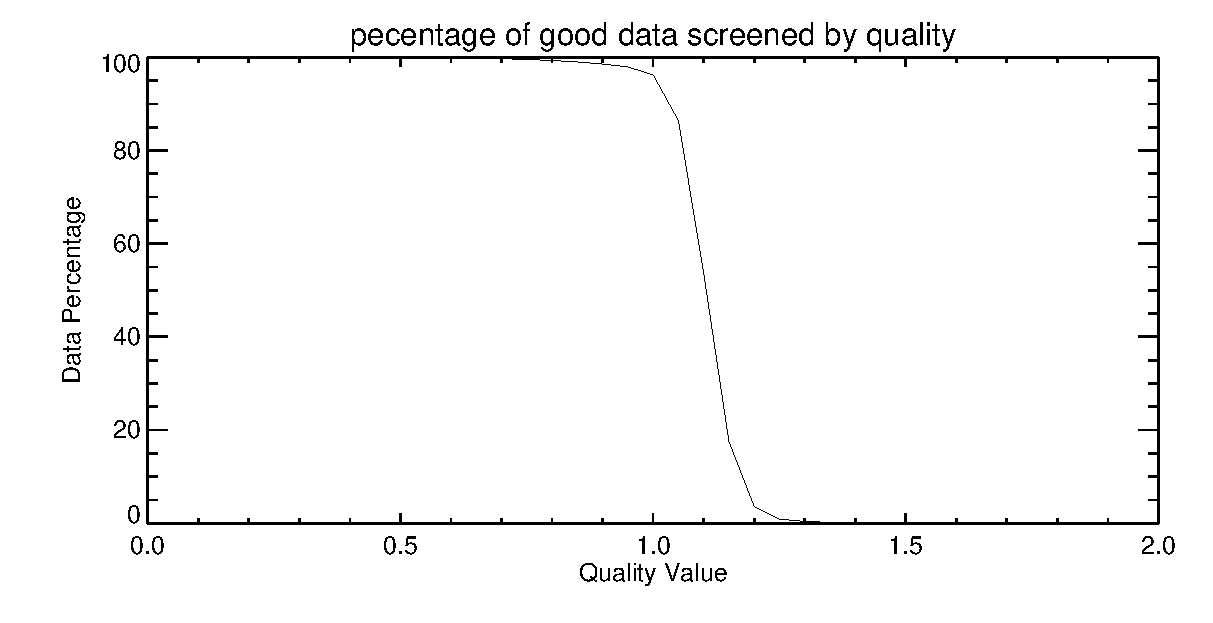
\includegraphics[width=0.8\linewidth]{figures/so2_data_yields}
\end{center}
\caption{Percentage of data having a quality greater than that indicated
  on the x-axis for v4.2 data processed for June--August 2005.}
\label{fig:so2datayields}
\end{figure}

\subsection*{Review of comparisons with other datasets}

MLS has successfully detected SO\cs2 from 23 eruptions since launch.
These include Manam (Papua, New Guinea -- 3 events), Anatahan (Mariana
Islands), Sierra Negra (Galapogos Island), Soufriere Hills (Montserrat,
West Indies -- 2 events), Tunguraua (Ecuador), Rabaul (Papua New
Guinea), Piton de la Fournaise (Reunion Island), Jebel al-Tair (Yemen),
Okmok (Alaska), Kasatochi (Alaska), Dalaffilla (Ethiopia), Redoubt
(Alaska), Sarychev (Kuril Islands, Russia), Pacaya (Guatamala), and
Merapi (Indonesia), Grimsvotn (iceland), Puyehue-Cordon Caulle, (Chile),
Nabro (Eritrea), Paluweh (Indonesia), Sangeang Api (Indonesia).

\begin{figure}
\begin{center}
\includegraphics[width=0.7\linewidth]{figures/sarychev_14062009}
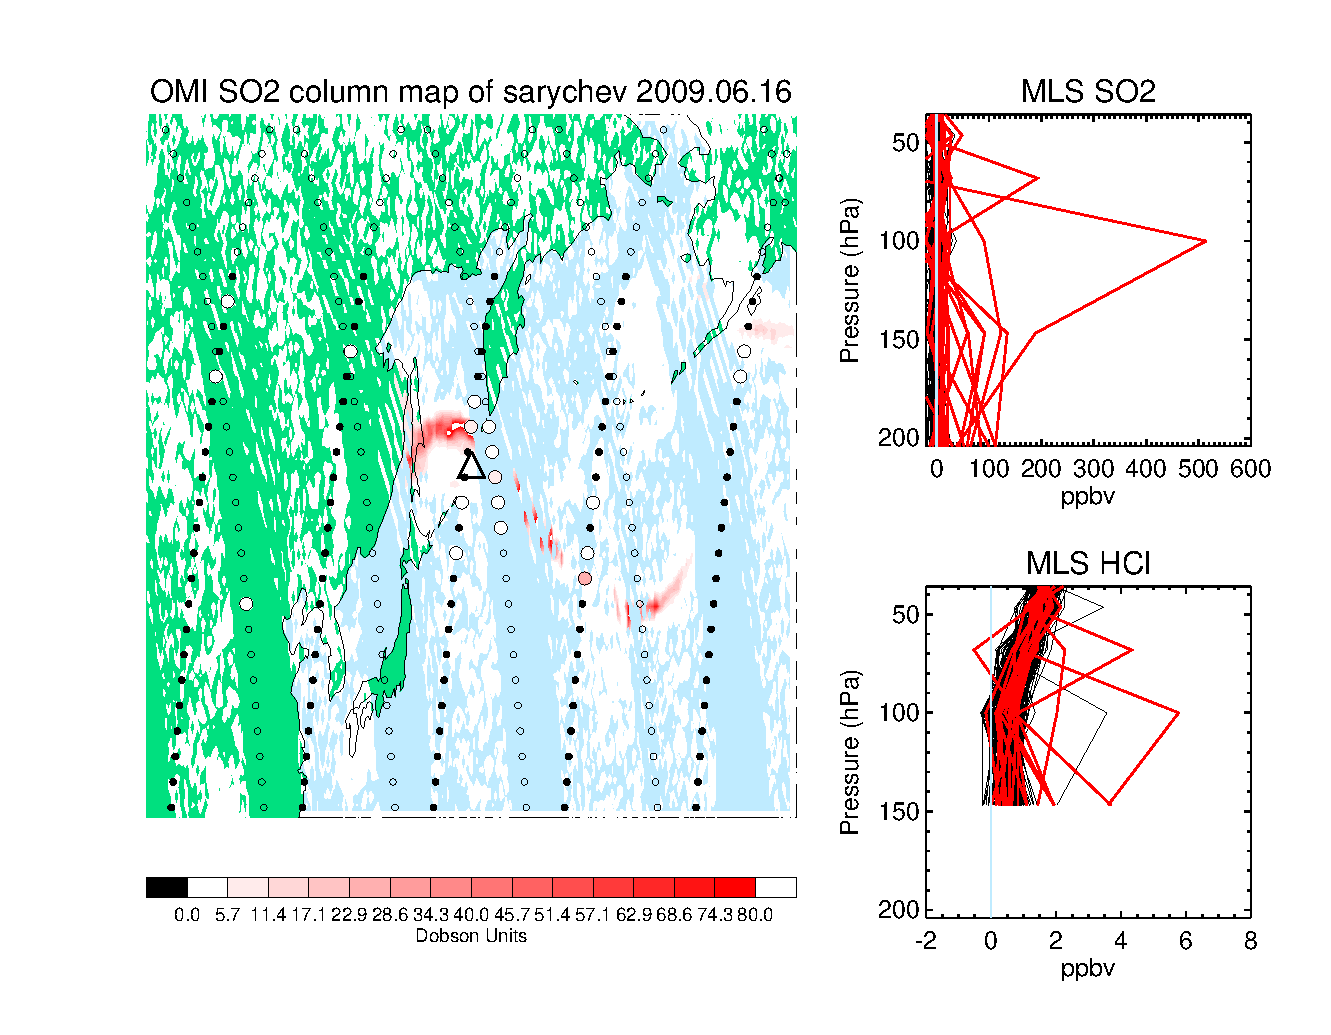
\includegraphics[width=0.7\linewidth]{figures/sarychev_16062009}
\end{center}
\caption{An overlay of MLS measurement tracks on an OMI SO\cs2
  measurement on 14 and 16 June 2009 (separate maps) showing the
  dispersial of SO\cs2 from the Sarychev eruption (13~June 2009, black
  triangle). The color scale indicates the SO\cs2 column measured by
  OMI\@. The daytime MLS tracks are small open circles and the nighttime
  tracks are filled black. When the calculated column from MLS exceeds
  1\,DU, that measurement is indicated by a larger open circle filled
  with the color of the column measurement as indicated by the color
  scale below (same as for OMI)\@. The panels at right show all the
  measured profiles covering the area shown in the maps for SO\cs2 and
  HCl. Profiles where the MLS column calculation exceeds 1\,DU are
  highlighted in red.}
\label{fig:so2overlay}
\end{figure}

Figure~\ref{fig:so2overlay} shows an overlay comparison of column SO\cs2
measured by OMI and the same calculated by MLS for two days following
the Sarychev eruption. It is clear that MLS detects the main plume
dispersal features. It also appears that MLS columns are often smaller
than those from OMI\@. Interpreting the significance of this is not
straightforward given that OMI has to make assumptions regarding the
profile shape and can observe SO\cs2 down to the boundary layer. The MLS
column begins at 215\,hPa and integrates upward neglecting the
tropospheric contributions. Another limitation is that OMI can only make
measurements during the day whereas MLS can make them day and night.
Since the plume is moving relatively quickly over the 12-hour
measurement separation time, MLS nighttime measurements often miss
and/or detect plume features differently than OMI\@.

Figure~\ref{fig:so2timeseries} shows a comparison between v4 and v3 for
a track showing the maximum SO\cs2 measured on 16~June 2009. Although both
version detect large amounts of SO\cs2 at 100\,hPa, v4 shows this being more
concentrated in the 100-hPa layer than v3, as the newer version shows less
SO\cs2 at 147\,hPa and none at 215\,hPa compared to v3. Neither version shows
any SO\cs2 at 68\,hPa.

\begin{figure}
\begin{center}
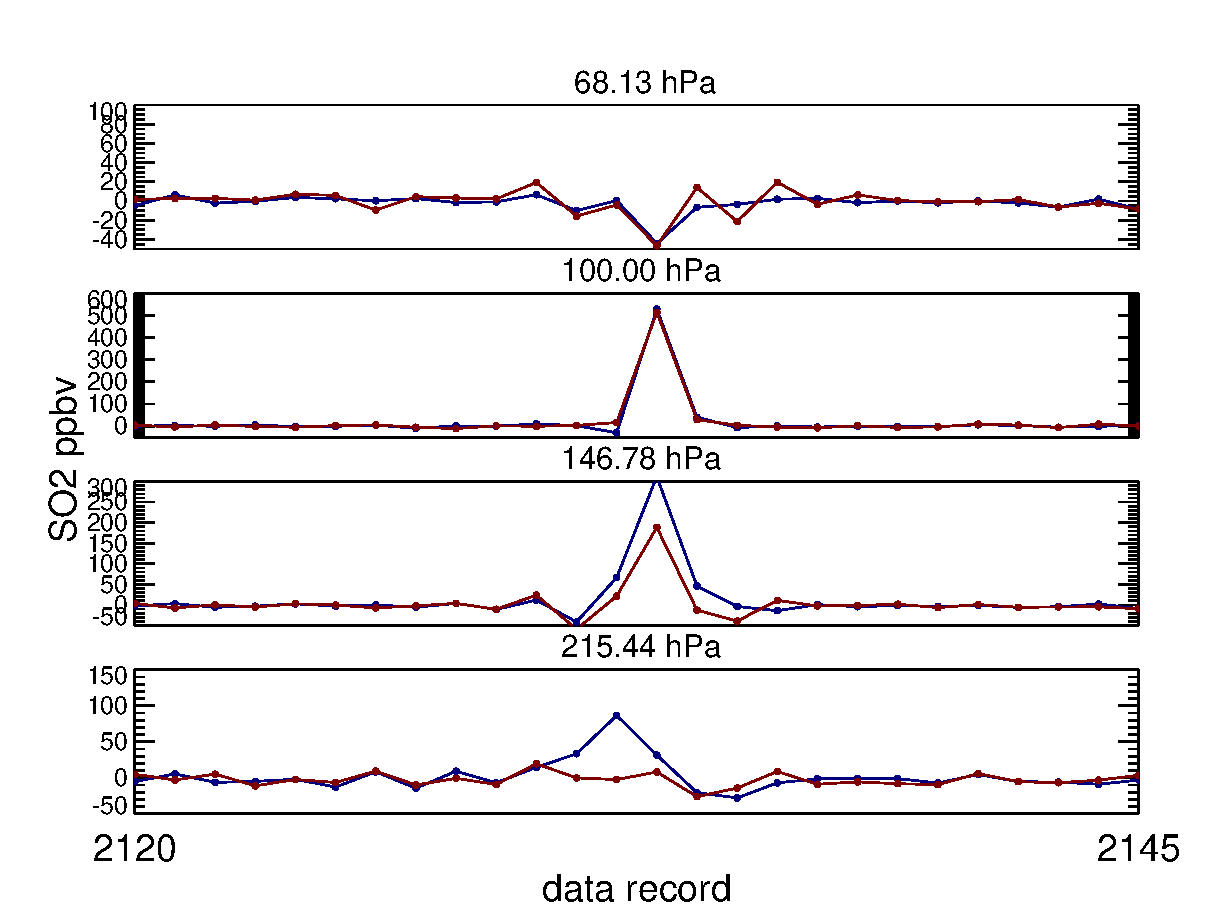
\includegraphics[width=0.7\linewidth]{figures/sarychev_time_series_20090616_2120}
\end{center}
\caption{Time series overlay where MLS measures more than 500\,ppbv at
  100\,hPa for the Sarychev erruption. Blue is version 3, and red is
  version 4.}
\label{fig:so2timeseries}
\end{figure}


\begin{table}
\caption{Summary of MLS v3.3 SO\cs2 product.}
\label{tab:SO2Summary}
\vspace{\tablecaptionsep}
\begin{minipage}{\linewidth}
\centering\begin{tabular}{ccccl}
\toprule
\parbox[m]{6em}{\bfseries\centering Pressure / hPa} &
\parbox[m]{6em}{\bfseries\centering Resolution V~$\times$~H \ km} &
\parbox[m]{8em}{\bfseries\centering Single profile precision} &
\parbox[m]{6em}{\bfseries\centering Accuracy / ppbv} &
\bfseries Comments \\
\midrule
$<$ 10 & --- & --- & --- &  Unsuitable for scientific use \\
10 & 3.1 $\times$ 165 &  4.5 &  6  & \\
15 & 3.1 $\times$ 171 &  5.0 &  3  & \\
22 & 3.1 $\times$ 171 &  4.4 &  4  & \\
32 & 3.0 $\times$ 176 &  3.8 &  5  & \\
46 & 2.9 $\times$ 176 &  3.5 &  5  & \\
68 & 2.9 $\times$ 183 &  3.3 &  6  & \\
100 & 2.8 $\times$ 180 &  3.2 &  6  & \\
147 & 2.8 $\times$ 180 &  2.5 &  10 & \\
215 & 3.5 $\times$ 186 &  3.5 &  20 & \\
$>$215 & --- & --- & --- & Unsuitable for scientific use \\
\bottomrule
\end{tabular}
\end{minipage}
\end{table}


%%% Local Variables:
%%% mode: latex
%%% TeX-master: "v4-x-report"
%%% End:
 \speciestitle{Temperature}{T}{Temperature}{%
\item[Useful range:] 261\,--\,0.001\,hPa
\item[Contact:] Michael J. Schwartz,
  \email{Michael.J.Schwartz@jpl.nasa.gov}}
\subsection*{Introduction}

The MLS \thisv temperature product is similar to both the v3.3 product
and to the v2.2 product that is described in~\citet{SchwartzEtal08}.
MLS temperature is retrieved primarily from bands near O\cs2 spectral
lines at 118\,GHz and 239\,GHz that are measured with MLS radiometers
R1A/B and R3, respectively.  The isotopic 239-GHz line is the primary
source of temperature information in the troposphere, while the 118-GHz
line is the primary source of temperature in the stratosphere and above.
MLS \thisv temperature has a \texttildelow$-1\,$K bias with respect to
correlative measurements in the troposphere and stratosphere, with
2\,--\,3\,K peak-to-peak additional systematic vertical structure.
Table~\ref{tab:TemperatureSummary} summarizes the measurement precision,
resolution, and modeled and observed biases.  The following sections
provide details.

\subsection*{Differences between \thisv and \prevvSlash}
Mean differences between \thisv temperature and \prevvSlash temperature
are typically less than 0.5\,K and exceed 1\,K only in the tropical
troposphere and, in some instances, at the highest retrieval levels, 
0.01--0.001\,hPa (see Figure~\ref{fig:v4T-v3T_2005}).  In the tropics, a cold
bias in unscreened \thisv relative to \prevv reaches 2\,K, and is
reduced to 1.5\,K by the recommended screening, discussed below.

Versions v3.x and v2.x take the standard temperature product from
\texttt{FinalPtan}, a preliminary ``phase'' of the MLS retrieval that
uses only the O\cs2 bands and that focuses on retrieval of temperature
and tangent-point pressure. The standard \thisv temperature product is
taken from the \texttt{CorePlusR3} phase, which adds radiances from the
240-GHz radiometer and which simultaneously retrieves standard products
for a number of atmospheric constituents.  The \texttt{CorePlusR3}
temperature and GPH along with the accompanying tangent-point
pressures, are used for all subsequent constituent retrievals, so they
are more internally consistent with the suite of constituent retrievals
than were the standard temperature and GPH products of previous
versions.

\begin{figure}
\centering\includegraphics[angle=-90,width=\linewidth]{figures/diffv4v3T_plot1bylat}
\caption{Temperature differences between \thisv and v03.30 standard
  products, screened per recommendations of this document (green) and
  unscreened (red).  2005 data are shown.  Top row is mean difference
  between versions, binned by latitude. Screening has a significant
  impact on mean values only at low latitudes in the troposphere.  The
  middle panel show considerably more scatter in unscreened data at
  the bottom of the retrieval, particularly at low latitudes.  Bottom 
  panels' difference between red and green lines is 
  the number of points that are screened out}
\label{fig:v4T-v3T_2005}
\end{figure}

MLS is generally insensitive to the presence of thin clouds, but
scattering in the cores of convective storms can produce significant
perturbations in MLS retrieved quantities.  Temperature is particularly
susceptible to ``significant'' perturbations, because \emph{a priori}
knowledge from analysis is generally good enough in much of the lower
and middle atmosphere that perturbations of a few percent (a level
negligible for trace-gas constituent retrievals) are considered
``significant'' for temperature.  In the troposphere where \emph{a
  priori} knowledge may be on the order of 1--2\,K, large differences
between MLS and GEOS-5 are believed to typically result from problems in
the MLS measurements.  Plotting differences between the MLS retrieved
temperatures and the GEOS-5 temperatures (the retrieval \emph{a priori}
in the UT and stratosphere) is often useful in identification of
retrieval artifacts.  Cloud-induced perturbations generally occur in the
tropics and mid-latitudes (where convective storms occur) in both the v3
and v4 retrieval versions, but perturbations of retrieved temperature
and the recommended screening for their removal have changed between
\prevvSlash and \thisv.  In unscreened data at retrieval levels
316\,--\,178\,hPa, clouds produce primarily positive outliers in \thisv and
negative perturbations in v03.30. The top panels of
Figure~\ref{fig:v4v3__215hPa_pcolorhist2} show this behavior at
215\,hPa. Conversely, at 121\,hPa, outliers are primarily negative in
v03.x and positive in \thisv.

\begin{figure}
\centering\includegraphics[width=0.7\linewidth]{figures/v4v3_215hPa_pcolorhist2}
\caption{The top row shows histograms of unscreened 215-hPa v03.30
  (left) and v04.20 (right) temperature differences from GEOS-5.9
  temperature from 2005 data.  The horizontal bin spacing is
  \texttildelow1.5\degsym\ latitudinal spacing of the repeating MLS scan
  pattern.  The bottom panels show histograms of analogous screened
  differences on a finer vertical scale.  Outliers beyond $\pm$20\,K
  have been almost completely eliminated and are not shown.}
\label{fig:v4v3__215hPa_pcolorhist2}
\end{figure}

Unscreened and screened histograms of tropical (20\degsym S--20\degsym
N) v03.30 and v04.20 temperature from 2005 are shown in
Figure~\ref{fig:v4v3_68-316hPa_linehists}.  Tails of low, unscreened
v04.20 outliers (dark red) are particularly evident from 316--147\,hPa,
but are greatly reduced by recommended screening (magenta).  Changes at
316\,--\,215\,hPa between v03.30 and \thisv in mean tropical temperature
differences from GEOS-5.9, given numerically in the upper left corners
of the panels, can be seen to reflect shifts in the peaks of the
distributions as well as the contributions of the outlier tails.



\begin{figure}
  \centering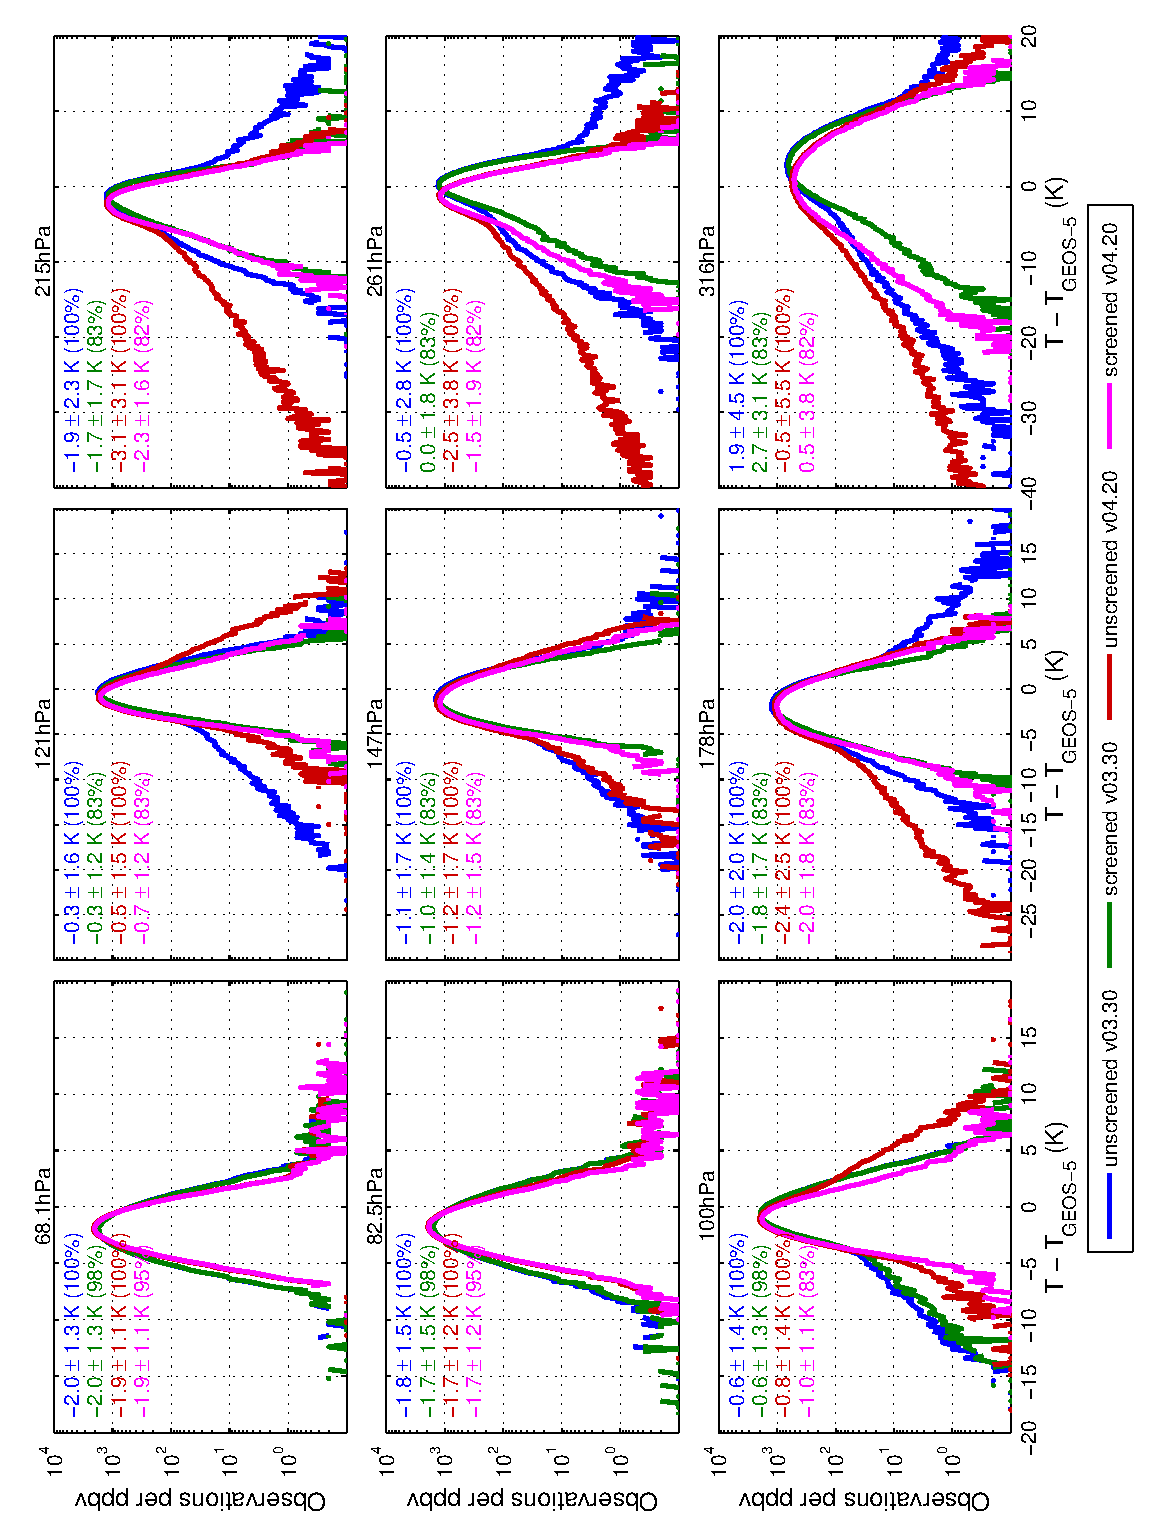
\includegraphics[angle=-90,width=\linewidth]{figures/v4v3_68-316hPa_linehists}
  \caption{Panels show histograms of tropical (20\degsym S--20\degsym N)
    differences between MLS retrieved temperatures and GEOS-5.9
    temperature for all of 2005.  Blue and green lines are unscreened
    and screened v03.30, respectively. Red and magenta are unscreened
    and screened v04.20, respectively.  Distribution means and standard
    deviations are given in the upper left of each panel along with the
    percentage of points included after screening.  The 316-hPa level is
    shown for reference although this level is not recommended to be
    used for scientific work.}
\label{fig:v4v3_68-316hPa_linehists}
\end{figure}

The tropospheric and stratospheric \emph{a priori} temperature profiles
used in \thisv are from GEOS-5.9, but are quite similar to the GEOS-5.7
and GEOS-5.2 profiles used in previous version, departing most
significantly near the stratopause.  This change in \emph{a priori}
temperature is believed to have only minimal impact on retrievals.

\subsection*{Resolution}
\onestandardavk{Temperature_HR}{Temperature}%

The vertical and horizontal resolution of the MLS temperature
measurement is shown by averaging kernels in
Figure~\ref{fig:AvkTemperature_HR}.  Vertical resolution, shown on the
left panel, is \texttildelow4.5\,km from 261\,hPa to 100\,hPa, improves
to 3.6\,km at 31.6\,hPa and then degrades to 4.3\,km at 10\,hPa, 5.5\,km
at 3.16\,hPa, 6\,km at 0.01\,hPa, and 8\,--\,10\,m at 0.01\,hPa.  Along
track resolution is \texttildelow165\,km from 261\,hPa to 0.1\,hPa and
degrades to 280\,km at 0.001\,hPa.  The cross-track resolution is set by
the 6-km width of the MLS 240-GHz field of view in the troposphere and
by the 12-km width of the MLS 118-GHz field of view in the stratosphere
and above.  The longitudinal separation of MLS measurements from a given
day, which is determined by the Aura orbit, is 10\degsym--\,20\degsym\
over middle and low latitudes, and finer in polar regions.

\subsection*{Precision}

The precision of the MLS \thisv temperature measurement is summarized in
Table~\ref{tab:TemperatureSummary}.  Precision is the random component
of measurements which would average down if the measurement were
repeated.  The retrieval software returns an estimate of precision based
upon the propagation of radiometric noise and \emph{a~priori}
uncertainties through the measurement system.  These values, which range
from 0.5\,K in the lower stratosphere to \texttildelow2.5\,K in the
mesosphere, are given, for selected levels, in column~2.  Column~3 gives
the rms of differences of values from successive orbits (divided by the
square-root of two as we are looking at the difference of two noisy
signals) for latitudes and seasons where longitudinal variability is
small and/or is a function only of local solar time.  The smallest
values found, which are in the tropics in the troposphere and in 
high-latitude summer in the stratosphere and mesosphere, are taken to be those
least impacted by atmospheric variability and are what is reported in
column~3.  These values are 0.5--0.8\,K larger than those estimated by the
measurement system in the troposphere and lower stratosphere, and a
factor of \texttildelow1.4 larger from the middle stratosphere through
the mesosphere.

\subsection*{Accuracy}

A substantial study of sources of systematic error in MLS measurements
was done as a part of the validation of v2.2, and as the measurement
system is substantially unchanged, those results are repeated here.  The
accuracy of the v2.2 temperature measurements was estimated both by
modeling the impact of uncertainties in measurement and retrieval
parameters that could lead to systematic errors, and through comparisons
with correlative data sets.  Column~5 of
Table~\ref{tab:TemperatureSummary} gives estimates from the propagation
of parameter uncertainties, as discussed in~\citet{SchwartzEtal08}.
This estimate is broken into two pieces.  The first term was modeled as
amplifier non-linearity, referred to as ``gain compression,'' and was
believed to have a known sign, as gain is known to drop at high
background signal levels. Correction of these nonlinearities was a goal
of \thisv, but closer examination of the simple non-linearity model
found that it did not close forword model and measured radiances as
expected.  It had been hoped that better radiance closure would permit
the use of more radiances in the middle of the 118-GHz O\cs2 band,
giving better resolution, precision and accuracy in the upper
stratosphere and better accuracy everywhere.  This work is still
ongoing, and it is hoped that advances will manifest in improvements in
a future version.

The second term of column~5 combines $2\sigma$ estimates of other
sources of systematic uncertainty, such as spectroscopic parameters,
retrieval numerics and pointing, for which the sign of resulting bias is
unknown.  Gain compression terms range from $-1.5\,$K~to~$+4.5$\,K, and
predicted vertical structure is very similar to observed biases relative
to correlative data in the troposphere and lower stratosphere.  The
terms of unknown sign are of \texttildelow2\,K magnitude over most of
the retrieval range, increasing to 5\,K at 261\,hPa and to 3\,K at
0.001\,hPa.

Column~6 contains estimates of bias based upon comparisons with analyses
and with other previously-validated satellite-based measurements.  In
the troposphere and lower stratosphere, the observed biases between MLS
and most correlative data sets are consistent to within
\texttildelow1.5\,K, and have vertical oscillation with an amplitude of
2\,--\,3\,K and a vertical frequency of about 1.5~cycles per decade of
pressure.  A global average of correlative measurements is shown in
Figure~\ref{fig:TempSummary2}.

\subsection*{Data screening}
\label{sec:TemperatureScreening}
\begin{description}
\item[Pressure range:] \screeningrule{261\,--\,0.001\,hPa} \standardrangestatement
\standardprecisionrule
\evenstatusrule

\item[Quality:] Only use profiles with \texttt{Quality}
    greater than 0.2 for the 83\,hPa level and smaller pressures, and
    profiles with \texttt{Quality} greater than 0.9 at larger pressures
    of 100\,hPa and larger.

    Profiles with \texttt{Quality} less than or equal to 0.9 comprise
    1.4\% of all data, and 4.8\% of profiles in the tropics.

\item[Convergence:] \convergencerule{1.03} This \texttt{Convergence}
  criterion rejects $<0.1\%$ of profiles and chunks with convergence
  slightly over this target do not contain manifestly pathological
  profiles.  The primary purpose of this criterion is to reject profiles
  with extremely poor convergence that may be expected to reflect poor
  retrieval behavior.

\item[Cloud Screening:] The ``low cloud'' bit of the temperature
  \texttt{Status} field does not contain useful information in \thisv,
  so it cannot be used to screen temperature as it was in previous
  versions.  However, cloud impacts can largely be removed using the ice
  water content (IWC) product, rejecting profiles between 261\,--\,100\,hPa
  for which the 215\,hPa value of IWC is greater than 0.005\,g/m$^3$.
  Implementation of this criteria requires the loading of the \thisv IWC
  swath, but is responsible for most of the rejection of cloud-induced
  outliers seen in Figure~\ref{fig:v4v3_68-316hPa_linehists}.  This
  criteria removes 4.7\% of UT profiles globally and 15\% of profiles in
  the tropics (20$^\circ$\,N--20$^\circ$\,S).

\item[Precision:] The \texttt{L2gpPrecision} field can be used to further
  eliminate outliers that are believed to be the result of thick clouds,
  primarily in the tropics.  If careful screening of the troposphere is
  required, levels 261\,--\,178\,hPa should be avoided if any of the
  following criteria are met:
\begin{description}
\item[At 316\,hPa:] \texttt{L2gpPrecision} $> 1.1$\,K \textbf{and} latitude $> -60\degsym$
\item[At 261\,hPa:] \texttt{L2gpPrecision} $>  0.7\,$K 
\item[At 215\,hPa:] \texttt{L2gpPrecision} $>  0.825\,$K 
\end{description}

\item[End of day (v4.20 only):] The last four profiles of each day show
  greatly increased rates of large departure from \emph{a priori} and
  should not be used.  This issue was fixed in v4.22.
\end{description}

\subsection*{Artifacts}
MLS temperature has persistent, vertically oscillating biases with
respect to analysis and correlative measurements in the troposphere and
stratosphere that are an area of continued research.  The impact of
clouds is generally limited to tropospheric levels and to the tropics
and, to a lesser extent, mid-latitudes.  Cloud impacts in unscreened
data at the lowest retrieved levels are larger in \thisv than they were
in \prevv and are harder to screen due to the lack of a useful ``low
cloud'' status bit.  However, after recommended screening, tropical
negative departures from \emph{a priori} of greater than 10\,K (believed
almost always to cloud-induced artifacts) are seen in only 0.2\% of
tropical profiles.  Flagging of clouds is discussed above.  Further
discussion of artifacts may be found in~\citet{SchwartzEtal08}.

The last four profiles of each day show increased rates of outliers
relative to GEOS-5 temperature, compared to other profile positions in
the day in version~4.20 (fixed in version~4.22).  These outliers can be
as large as 50\,K at at some levels.  A recommendation to discard the
last 4 profiles of each day has been added to recommended screening for
v4.20 (not needed for v4.22).

\subsection*{Review of comparisons with other datasets}
\label{sec:TComparisons}

\begin{figure}
\centering\includegraphics[width=0.7\linewidth]{figures/TempSummary2}
\caption{The left panel shows globally-averaged mean differences between
  MLS temperature and eight correlative data sets.  Criteria for
  coincidences are described in detain in~\citet{SchwartzEtal08}.  The
  right panel shows the global standard deviations about the means.}
\label{fig:TempSummary2}
\end{figure}

\begin{figure}
\centering\includegraphics[width=0.7\linewidth]{figures/binbylat_v4-ap_2005}
\caption{Zonal mean of the difference between MLS \thisv temperature and
  GEOS-5.9 temperature (upper), and variability
  about that mean (lower), averaged for 2005.}
\label{fig:MLSminusGEOS5_zonalmean}
\end{figure}

\sloppypar\citet{SchwartzEtal08} describes detailed comparisons of MLS v2.2
temperature with products from the Goddard Earth Observing System,
version~5~\citep{ReineckerEtal07} (GEOS-5), the European Center for
Medium-Range Weather Forecast~\citep[e.g.,][]{SimmonsEtal05} (ECMWF),
the {CHAllenging Minisatellite Payload} (CHAMP)~\citep{WickertEtal01},
the combined Atmospheric Infrared Sounder / Advanced Microwave Sounding
Unit (AIRS/AMSU), the Sounding of the Atmosphere using Broadband
Radiometry (SABER)~\citep{MlynczakAndRussell95}, the Halogen Occultation
Experiment~\citep{HervigEtal96} (HALOE) and the Atmospheric Chemistry
Experiment~\citep{BernathEtal04} (ACE), as well as to radiosondes from
the global network.  From 261\,hPa to \texttildelow10\,hPa there is
generally agreement to \texttildelow1\,K between the assimilations
(ECMWF and GEOS-5) and AIRS, radiosondes and CHAMP, with SABER and ACE
having generally warm biases of \texttildelow2\,K relative to this
group.  Figure~\ref{fig:TempSummary2} shows the global mean biases in
the left panel and the 1\,$\sigma$ scatter about the mean in the right
panel for these eight comparisons.  Between 1\,hPa and 0.001\,hPa, MLS
has biases with respect to SABER of $+$1\,K~to~$-$5\,K between 1\,hPa
and 0.1\,hPa, of 0\,K~to~$-$3\,K between 0.1\,K and 0.01\,K and
increasing in magnitude to $-$10\,K at 0.001\,hPa.  Estimates of
systematic error in the MLS temperature are shown in black, with
$2\sigma$ uncertainty shown with gray shading.  The black line is the
modeled contribution of ``gain compression,'' which was hoped would
explain much of the vertical structure of MLS biases in the upper
troposphere and lower stratosphere.  As discussed above, the
gain-compression model used in this study does not adequately close the
retrieval's radiance residuals, so further study is needed to understand
the forward-model inadequacies.

The upper panel of Figure~\ref{fig:MLSminusGEOS5_zonalmean} shows
zonal-mean differences between \thisv temperature and GEOS-5.9
temperature, averaged over 2005; the lower panel is the $1\sigma$
variability about that mean.  Persistent vertical structure in the
troposphere and lower stratosphere is evident, with the oscillations
somewhat stronger at the equator and poles than at mid-latitudes.  In
the upper stratosphere, MLS has a general warm bias relative to GEOS-5
at mid and high latitude that increases to more than 10\,K in the poles
at 1\,hPa.  The bias at 1\,hPa is much smaller in polar summer, but
persists in polar winter.

\begin{sidewaystable}
\caption{Summary of MLS Temperature product}\vspace{0.5ex}
\label{tab:TemperatureSummary}
\begin{minipage}{\textheight}
\centering\begin{tabular}{ccccccl}
\toprule
\textbf{Pressure} & 
\parbox[m]{4.5em}{\centering\textbf{Precision\footnote{Precision on individual profiles} \\/ K}} &
\parbox[m]{4em}{\centering\textbf{Observed Scatter\footnote{Precision
      inferred from differences of
      individual profiles from successive orbits (v2.2 results shown)} \\/ K}} &
\parbox[m]{4.5em}{\centering\textbf{Resolution\\ V $\times$ H\\ / km}} &
\parbox[m]{6em}{\centering\textbf{Modeled Bias\\uncertainty\\ / K}} &
\parbox[m]{6em}{\centering\textbf{Observed Bias\\uncertainty\\ / K}} &
\textbf{Comments} \\
\midrule
$<$0.001\,hPa      & ---       & ---      &  ---             & --- & --- & Unsuitable for scientific use \\
0.001\,hPa         & $\pm$3.6  & $\pm$3.5 & 11--14 $\times$ 280 & $+$2\,$\pm$\,3    & $-$9     & \\
0.01\,hPa          & $\pm$3.3  & $\pm$3   & 10--11 $\times$ 260 & $+$2\,$\pm$\,3    & $-$2\,to\,0 & \\
0.1\,hPa           & $\pm$2.4  & $\pm$2.7 & 6   $\times$ 170 & $+$2\,$\pm$\,2    & $-$8\,to\,0 & \\
0.316\,hPa         & $\pm$1.3  & $\pm$1.5 & 8   $\times$ 170 & $+$3\,$\pm$\,2    & $-$7\,to\,$-$4& \\
1\,hPa             & $\pm$1.2  & $\pm$1.3 & 6.8 $\times$ 165 & $+$1\,$\pm$\,2    &  0\,to\,$+$5 & \\
3.16\,hPa          & $\pm$0.8  & $\pm$0.8   & 5.5 $\times$ 165 & $+$2\,$\pm$\,2    & $+$1 & \\
10\,hPa            & $\pm$0.6  & $\pm$0.7   & 4.1 $\times$ 165 &  0\,$\pm$\,2      & $-$1\,to\,0& \\
14.7\,hPa          & $\pm$0.6  & $\pm$0.7   & 3.9 $\times$ 165 & $+$4\,$\pm$\,2    &  0\,to\,$+$1 & \\
31.6\,hPa          & $\pm$0.5  & $\pm$0.6   & 3.6 $\times$ 165 & $+$1\,$\pm$\,2    & $-$2\,to\,0 & \\
56.2\,hPa          & $\pm$0.6  & $\pm$0.7 & 3.8 $\times$ 165 & $-$1\,$\pm$\,2    & $-$2\,to\,0 & \\
100\,hPa           & $\pm$0.7  & $\pm$1.0 & 4.6 $\times$ 165 & $+$2\,$\pm$\,2    &  0\,to\,$+$1  & \\
215\,hPa           & $\pm$0.8  & $\pm$1.2   & 3.5 $\times$ 165 &  $-$1.5\,$\pm$\,4 & $-$2.5\,to\,$-$1.5   & \\
261\,hPa           & $\pm$0.7  & $\pm$1.5   & 4.0 $\times$ 167 &  0\,$\pm$\,5      & $-$2\,to\,0   & \\
1000\,--\,316\,hPa & ---       & ---      & ---              & ---           & --- & Unsuitable for scientific use\\
\bottomrule
\end{tabular}
\end{minipage}
\end{sidewaystable}

%%% Local Variables: 
%%% mode: latex
%%% TeX-master: "v4-x-report.tex"
%%% End: 

 
\clearpage

%%% Local Variables: 
%%% mode: latex
%%% TeX-master: "v4-x-report"
%%% End: 
 \clearpage
\renewcommand{\currentnav}{BLANK}
%
\renewcommand{\leftmark}{Bibliography}
\renewcommand{\rightmark}{Bibliography}
\bibliography{shortnames,mybib}
%
\end{document}

%%% Local Variables: 
%%% mode: latex
%%% TeX-master: t
%%% End: 
